\section{Introduction}

\subsection{Motivation and Strategic Context}
Indianapolis 500 qualifying creates an unusual motorsport decision problem because a completed qualifying run is not necessarily the end of a car's session. Once a car has established an official four-lap qualifying result, the team may still attempt to improve that result later in the session. The strategic difficulty is that different routes to another attempt carry different forms of risk. At a simplified operational level, the team faces a trade-off between two possibilities. First, it may sacrifice the security of the current qualifying result in exchange for greater priority for another run. By withdrawing the existing result and entering the priority queue, the team may obtain an earlier opportunity to return to the track, but the current benchmark is no longer protected. Second, it may retain the current result and wait in the lower-priority queue. This protects the existing qualifying position, but introduces a different set of risks. Another opportunity may not arrive before the session closes, and even if it does, the physical environment may have changed substantially by the time the car returns to the circuit. The resulting decision is therefore not simply

\begin{center}\textit{Will another attempt be faster?}\end{center}

It is closer to

\begin{center}\textit{preserve the current result and wait}\end{center}

versus

\begin{center}\textit{sacrifice the current result for priority and reattempt earlier.}\end{center}

The full decision combines competitive position, queue structure, remaining session time, competitor behaviour, vehicle state, driver and engineering judgement, and changing environmental conditions. Among these components, the evolution of the physical environment is particularly important because Indianapolis qualifying performance is sensitive to thermal conditions. Track-surface temperature can change materially during a session, while ambient conditions and the broader thermal environment evolve simultaneously. A later qualifying opportunity is therefore not physically equivalent to the attempt that has just been completed. A team considering whether to retain its current result is consequently exposed to two conceptually different forms of uncertainty.

The first is opportunity uncertainty: another attempt may not become available at all, or may become available only after a substantial wait. The second is performance-state uncertainty: conditional on another opportunity becoming available, the track and atmospheric state may have changed enough to alter the car's achievable four-lap performance. This distinction ultimately became central to the project.

\subsection{Original Research Direction and Identifiability Problem}
The original research direction was broader than the final model. Because repeat qualifying attempts depend operationally on when a car can return to the track, queue waiting time initially appeared to be a natural modelling target. A complete strategy-support system might ideally estimate when another opportunity would occur and then estimate what performance would be achievable at that time. Considerable effort was therefore devoted to reconstructing attempt chronology, Lane 1 and Lane 2 behaviour, withdrawals, pit returns, requeue events, repeat-attempt structure and timing. Historical investigation showed, however, that these variables were not recorded consistently enough across seasons. Indianapolis 500 archives provide substantial information about official four-lap results and, in some seasons, repeated qualifying attempts. They do not provide a uniformly complete record of queue entry, lane state, withdrawal timing, requeue behaviour, live queue position, team intent or exact future-opportunity timing across the historical period required for statistical modelling. Team intent is particularly problematic because even when an action can be observed, the reasoning that produced that action generally cannot. Historical waiting time therefore could not be reconstructed consistently enough to serve as a defensible supervised-learning target. This was not simply a missing-data inconvenience. It changed the statistical formulation of the project. Rather than constructing a weakly labelled queue-time model and introducing false precision, future on-track opportunity time was reformulated as a conditional scenario axis. The project therefore stopped trying to answer

\begin{center}\textit{When will the next qualifying opportunity occur?}\end{center}

from incomplete historical queue evidence. Instead, it asks:

If another on-track opportunity occurs h minutes from now, what distribution of four-lap qualifying-performance change should be expected relative to the car's current official result?

The scientific inference target is therefore

\begin{center}\textit{p (\ensuremath{\Delta}v | H = h, current physical state, future environmental scenario) ,}\end{center}

where H denotes the time at which another on-track opportunity becomes available. The model estimates

\begin{center}\textit{p(\ensuremath{\Delta}v | H = h),}\end{center}

not

\begin{center}\textit{P (H = h).}\end{center}

This distinction separates two problems that initially appeared to belong in a single model:

\begin{center}\textit{future opportunity process}\end{center}

and

\begin{center}\textit{future physical-performance process.}\end{center}

The first could not be reconstructed historically with sufficient confidence. The second could. This distinction defines the final scope of the project. The frozen scientific inference system is calibrated at five future opportunity horizons:

\begin{center}\textit{Hcal = \{15, 30, 60, 90, 120\} minutes.}\end{center}

These horizons represent conditional future opportunity scenarios rather than predicted queue waiting times. Real qualifying opportunities can, however, occur at arbitrary times between the calibrated anchors. For this reason, the final implementation also contains a separate derived operational visualization layer that connects the calibrated outputs across the supported 15--120 minute range. The distinction is therefore

\begin{center}\textit{scientific calibration resolution \ensuremath{\neq} operational visualization resolution.}\end{center}

In a live setting, queue information, Lane 1 and Lane 2 state, remaining session time and leaderboard position can be interpreted against this operational performance curve. If live information suggests that another opportunity is plausible within a particular future interval, the corresponding section of the curve can be inspected without requiring the physical model itself to predict queue duration. The model therefore contributes evidence to the original strategic problem without claiming to reproduce the complete pit-wall decision.

\subsection{Historical Data Reconstruction as Part of the Problem}
The physical-performance problem could not be approached using a conventional ready-made dataset. The historical data required for the project did not exist as a single consistent attempt-level table. Evidence instead had to be reconstructed across multiple seasons from heterogeneous and partially overlapping sources. Official qualifying results provided classified performance information but did not always expose the full sequence of repeat attempts. Detailed timing reports contained additional information at different levels of granularity. Section and trap reports contained fields such as S1, S2A, S2B, S3A, S3B, S4A, S4B, S5A and S5B, together with T1--T4 and related measurements. These records became useful not only as performance information but as reconstruction evidence. They could help determine whether a car had started, progressed through or completed an attempt even when the complete run was not represented cleanly elsewhere.

Attempt identity, chronology, driver, run order, official four-lap average, section timing, environmental observations and repeat-attempt relationships therefore had to be reconciled across separate sources. The project consequently developed into an evidence-engineering problem as well as a modelling problem. Historical records were assigned different evidential roles depending on their completeness and reliability. Ambiguous attempt identities or chronology were not resolved merely to increase sample size. Where a unique reconstruction could not be defended, the record was quarantined or excluded from the frozen modelling core. This produced a relatively small final core compared with the volume of historical material investigated. The small sample is therefore partly a consequence of the methodological choice to prefer defensible transitions over nominal sample size. The final frozen 2020--2024 performance core contained

evidence-qualified same-car transitions. The unit of analysis was deliberately kept at the level of one complete four-lap qualifying attempt. The four constituent laps were not treated as four independent observations because doing so would artificially enlarge the dataset while ignoring their strong within-run dependence. The reconstruction process therefore established a broader methodological principle used throughout the project:

\begin{center}\textit{more historical records \ensuremath{\neq} more defensible modelling evidence.}\end{center}

\subsection{Why Same-Car Performance Change Became the Core Target}
The primary evidence source for performance modelling became the same-car repeat qualifying attempt. For two chronologically ordered attempts by the same car,

\begin{center}\textit{\ensuremath{\Delta}v = v2 - v1 ,}\end{center}

where v denotes official four-lap average speed. This differential formulation was preferred to modelling absolute speed across unrelated cars. Comparing a car with itself removes much of the persistent variation associated with driver identity, chassis, engine package, underlying competitiveness and baseline setup. The current official result therefore becomes a same-day performance anchor rather than requiring the model to infer the absolute capability of the current car from historical vehicles. The modelling problem changes from

\begin{center}\textit{How fast is this car?}\end{center}

to

How might the performance already demonstrated by this car change as the physical environment changes?

This distinction is fundamental to the final system. Day 1 qualifying provided the principal source of same-car transitions.

Last Chance qualifying was also reconstructed as a separate evidence branch because it contains genuine official four-lap attempts and can provide repeated-run evidence. However, its field composition, competitive context and operational incentives differ from normal Day 1 qualifying, so it was not automatically treated as interchangeable with the primary evidence. Fast Friday was investigated for similar reasons. It provides high-performance running immediately before qualifying under qualifying-relevant engine and aerodynamic conditions, but practice run plans, traffic, tow conditions, tyre preparation and fuel state are less constrained than in official qualifying. It therefore became auxiliary evidence rather than a direct substitute for official same-car qualifying transitions. The guiding evidence hierarchy became approximately

same-car official qualifying repeats > contextually related qualifying evidence > Fast Friday / auxiliary evidence > field-wid

\subsection{Variable Investigation and Selection}
A much wider set of variables was considered than ultimately appeared in the core model. Candidate environmental variables included track-surface temperature, ambient temperature, wind and gusts, solar loading, cloud cover, humidity, atmospheric pressure, dew point and derived air density. Potential car-state variables included tyre preparation, tyre temperature and wear, setup changes, fuel state and driver execution. Track and ambient temperature were retained as the principal deterministic variables in the physical-response model because they combined three properties that were important to the project:

1. they could be reconstructed with comparatively high historical consistency;

2. they had a defensible physical relationship with qualifying performance;

3. they could be connected to a future-state forecasting problem.

Other variables were not rejected because they were physically irrelevant. Wind and gusts can affect aerodynamic balance and straight-line performance, but fixed historical weather observations cannot reconstruct the instantaneous and spatially varying wind field experienced by an individual car around the oval. The later V2-C diagnostic therefore investigated available wind proxies explicitly. The resulting evidence did not provide sufficiently stable cross-year support to justify an explicit deterministic or heteroskedastic wind term. This does not imply that wind has no physical effect. It means that

\begin{center}\textit{physical relevance \ensuremath{\neq} sufficient historical evidence for explicit modelling.}\end{center}

Solar radiation, cloud cover and local shading can strongly influence track heating, but attempt-level shade exposure could not be reconstructed reliably enough to support a direct solar term in the performanceresponse regression. Solar information instead entered the future track-state problem through the physically ordered pathway

\begin{center}\textit{solar state \ensuremath{\rightarrow} track heating \ensuremath{\rightarrow} Ttrack \ensuremath{\rightarrow} performance.}\end{center}

Mean solar state over the future interval was ultimately retained in the final future track-temperature model because it improved out-of-year performance. Humidity, pressure, dew point and air density were investigated as auxiliary or diagnostic variables. A density-only representation was not adopted because it would combine several atmospheric pathways while failing to represent the distinct role of track-surface temperature. Tyre preparation, tyre temperature, tyre wear, setup changes and driver execution clearly affect qualifying performance but cannot be reconstructed consistently at attempt level from the public historical record. Fuel load occupies an intermediate case. Exact quantities are not publicly observable, but a four-lap maximum-performance qualifying run creates a strong incentive to minimise unnecessary fuel mass. Fuel variation was therefore treated as constrained but not zero, and ultimately as part of residual performance variation rather than a primary deterministic predictor. The final feature set was therefore intentionally smaller than the set of physically relevant variables. The selection principle was

physical importance + historical observability + reconstruction confidence + cross-year support,

rather than physical plausibility alone.

\subsection{Physical Performance Rather Than Strategy Imitation}
The final physical-response problem is

\begin{center}\textit{(\ensuremath{\Delta}Ttrack , \ensuremath{\Delta}Tambient ) \ensuremath{\rightarrow} \ensuremath{\Delta}v.}\end{center}

This is deliberately different from learning historical team actions. The model does not infer that because a historical team withdrew a result, a future team should do the same. Historical team decisions contain hidden information about risk tolerance, setup, driver feedback, competitors, internal forecasts and objectives that cannot be recovered consistently. Instead, the project isolates one identifiable question:

How does the physical attractiveness of a possible future qualifying attempt change as the measurable environment evolves?

The core performance model is therefore constrained to describe physical-state change rather than historical strategy behaviour. It takes the form

\begin{center}\textit{\ensuremath{\Delta}v = \ensuremath{\beta}track \ensuremath{\Delta}Ttrack + \ensuremath{\beta}ambient \ensuremath{\Delta}Tambient + \ensuremath{\epsilon}.}\end{center}

No deterministic intercept is included. This encodes the condition

\begin{center}\textit{\ensuremath{\Delta} modelled physical state = 0    \ensuremath{\Rightarrow}     \ensuremath{\Delta}v}\end{center}

\begin{center}\textit{ˆ physical = 0.}\end{center}

The purpose is not to claim that two runs under identical measured temperatures must produce identical realised speeds.

Instead, the zero-intercept structure prevents the model from learning a generic ``reattempt bonus'' or ``reattempt penalty'' and attributing unobserved effects such as driver adaptation, tyre preparation or setup changes to the deterministic physical model. Those effects remain possible, but are represented as unexplained realised-performance variation.

\subsection{Separating Current Performance from Future Physical State}
Predicting future performance requires a second problem to be solved. Future track-surface temperature cannot simply be replaced by future ambient forecast temperature. The track possesses thermal inertia, and its future state depends on its current thermal condition as well as subsequent environmental evolution. The project therefore separates two models. The first estimates physical performance response:

\begin{center}\textit{(\ensuremath{\Delta}Ttrack , \ensuremath{\Delta}Tambient ) \ensuremath{\rightarrow} \ensuremath{\Delta}v.}\end{center}

The second estimates future track state. The final retained future-state interface is

\begin{center}\textit{(h, \ensuremath{\Delta}Tambient (h), G0 , Smean (h)) \ensuremath{\rightarrow} p (\ensuremath{\Delta}Ttrack (h)) ,}\end{center}

where

\begin{center}\textit{G0 = Ttrack,0 - Tambient,0}\end{center}

represents the current track-to-ambient thermal gap and

\begin{center}\textit{Smean (h)}\end{center}

represents mean solar state over the future interval. The complete scientific inference chain is therefore

current official result + current thermal state + future ambient trajectory + future solar state

\begin{center}\textit{\ensuremath{\Downarrow}}\end{center}

\begin{center}\textit{future track-state distribution}\end{center}

\begin{center}\textit{\ensuremath{\Downarrow}}\end{center}

\begin{center}\textit{future qualifying-performance distribution.}\end{center}

This structure allows the current car's demonstrated performance to remain the anchor while historical evidence is used primarily to estimate sensitivity to changing physical state. It also preserves the distinction between

\begin{center}\textit{future environmental input}\end{center}

and

\begin{center}\textit{qualifying-performance response.}\end{center}

\subsection{Uncertainty as Part of the Model Rather Than an Afterthought}
A deterministic prediction would give a misleading impression of precision. Thermal conditions explain only part of realised qualifying performance. Tyre preparation, setup changes, driver execution, transient wind, fuel state, mechanical variation and other unobserved factors remain. The final scientific inference system therefore distinguishes

\begin{center}\textit{expected physical contribution}\end{center}

from

\begin{center}\textit{unexplained realised-performance variation.}\end{center}

It also separates several uncertainty sources rather than collapsing them into one undifferentiated error term. Bootstrap variation represents uncertainty in the estimated physical-response coefficients. Future-track-state uncertainty represents uncertainty in how the track thermal state will evolve. Empirical out-of-year residual variation represents realised qualifying-performance changes that are not explained by the measured thermal variables. These three internal components are propagated jointly through Monte Carlo simulation. At each calibrated horizon

\begin{center}\textit{h ∈ \{15, 30, 60, 90, 120\},}\end{center}

the system produces quantities including

\begin{center}\textit{E[\ensuremath{\Delta}vphysical (h)],}\end{center}

predictive intervals, and

\begin{center}\textit{P (\ensuremath{\Delta}v(h) > 0).}\end{center}

These quantities are first generated at the five calibrated scientific anchors. A separate derived operational layer,

\begin{center}\textit{OPERATIONAL\_CURVE\_V2,}\end{center}

then connects the frozen anchor summaries over the supported 15--120 minute range for operational visualization. Intermediate minute-level outputs are therefore not independently calibrated predictive horizons.

They are explicitly labelled as

\begin{center}\textit{INTERPOLATED\_OPERATIONAL,}\end{center}

while the five scientific anchors are labelled

\begin{center}\textit{CALIBRATED\_ANCHOR.}\end{center}

The present state at

\begin{center}\textit{h=0}\end{center}

is retained only as

\begin{center}\textit{CURRENT\_STATE\_BOUNDARY,}\end{center}

not as a probabilistic future forecast. The distinction is therefore

\begin{center}\textit{scientific calibration \ensuremath{\neq} operational interpolation .}\end{center}

The final output remains probabilistic rather than a deterministic statement that another attempt will or will not be faster.

\subsection{Technical Regimes and Operational Applicability}
The central inference core was estimated from the 2020--2024 technical regime. Additional historical work extended both backward and forward across regulation eras, but these observations were not simply pooled into the training set to increase sample size. Pre-Aeroscreen evidence from 2018--2019 was investigated to examine whether the inferred physical relationship depended strongly on the reference technical package. The 2019 sample provided sufficient clean evidence for quantitative comparison, whereas 2018 produced insufficient defensible repeat-attempt evidence after reconstruction and filtering. The 2025 hybrid era then provided a stronger forward test and an external evaluation opportunity for the already-frozen 2020--2024 inference core. This created an important distinction between two different forms of generalisation. The first is physical transferability: whether the inferred thermal-performance relationship remains useful when the technical package changes. The second is operational applicability: whether the qualifying format still creates the strategic situation for which the decision-support system was designed. These are not equivalent. A physical relationship may remain plausible under a new car specification while a changed qualifying format removes or substantially alters the retain-versus-withdraw decision itself. Event-specific or future qualifying-format changes should therefore be treated as applicability conditions rather than assumed to preserve the historical decision structure automatically. The final system consequently separates

\begin{center}\textit{technical-regime transferability}\end{center}

from

\begin{center}\textit{qualifying-format applicability.}\end{center}

A functioning physical model should not be interpreted as an operationally relevant decision-support system if the repeat-attempt decision itself is absent.

\subsection{Research Questions}
The final project can be summarised through four research questions.

1. RQ1: Historical reconstruction.

Can fragmented Indianapolis 500 qualifying, repeat-attempt and environmental records be reconciled into a defensible same-car dataset for physics-conditioned performance analysis?

2. RQ2: Physical response.

Can changes in measurable thermal conditions explain a stable component of four-lap same-car qualifying-performance change across seasons?

3. RQ3: Future physical state and probabilistic outlook.

Given the current thermal state and a future environmental trajectory, can future track state and the resulting qualifying-performance distribution be estimated at operationally relevant, empirically calibrated future horizons?

4. RQ4: Transferability and applicability.

How well does a frozen reference-era inference system transfer to qualifying attempts from a later technical regime, and how should changes in qualifying format constrain the operational interpretation of the system?

These questions deliberately stop short of asking whether the model can directly optimise the withdrawversus-retain decision. The broader decision depends on information outside the historically identifiable dataset, including queue availability, current leaderboard position, competitors, driver feedback and team-specific risk tolerance. Figure 1 summarises the identifiability-driven reformulation from the original end-to-end strategy problem to the conditional physical-performance inference task.

Figure 1: Identifiability-driven reformulation of the original requalification strategy problem and the resulting final decision-support architecture.

\subsection{What the Project Ultimately Became}
The final project is therefore not a qualifying-strategy imitation model and not an automated pit-wall recommender. It is a physics-conditioned probabilistic performance-inference system built around an identifiability-driven decomposition of a larger strategy problem. Its main components are:

1. reconstruction and evidence engineering across fragmented multi-season qualifying records;

2. an evidence hierarchy and quarantine process for separating defensible modelling records from ambiguous historical material;

3. an identifiability-driven decision not to model historical queue duration from weak labels;

4. treatment of future opportunity time as a conditional scenario axis;

5. same-car differencing to anchor future inference to demonstrated current performance;

6. a zero-intercept physical-response model relating thermal-state change to four-lap speed change;

7. a separate future track-state model using future horizon, ambient evolution, current thermal gap and mean solar state;

8. explicit separation of future-state, coefficient and unexplained realised-performance uncertainty;

9. Monte Carlo propagation at the calibrated horizons

\begin{center}\textit{15, 30, 60, 90, 120 minutes;}\end{center}

10. a separately derived continuous operational visualization layer that connects the frozen calibrated summaries without claiming independent minute-level validation; 11. an external queue-context architecture in which live information can define a plausible opportunity window without requiring the physical model to estimate

\begin{center}\textit{P (H | Q);}\end{center}

12. cross-regime and external evaluation without retroactively enlarging the frozen inference core; 13. explicit separation between technical-regime transferability and qualifying-format applicability.

The complete conceptual structure can therefore be expressed as

real strategy problem \ensuremath{\rightarrow} historical identifiability analysis \ensuremath{\rightarrow} physically identifiable subproblem \ensuremath{\rightarrow} probabilistic performance

rather than

\begin{center}\textit{historical team actions \ensuremath{\rightarrow} predicted strategy action.}\end{center}

The final implementation adds a second distinction between scientific inference and operational presentation:

\begin{center}\textit{FINAL\_V2 \ensuremath{\rightarrow} five calibrated performance distributions}\end{center}

followed by

\begin{center}\textit{OPERATIONAL\_CURVE\_V2 \ensuremath{\rightarrow} derived continuous operational visualization.}\end{center}

Live queue and pit-wall context may then identify which portion of the operational curve is currently relevant. The system therefore answers one deliberately narrower but defensible question:

If another qualifying opportunity becomes available after a specified amount of time, how might the physical performance opportunity have changed relative to the car's current official result?

That answer can then be combined with live queue information, leaderboard state, competitor behaviour, driver feedback and engineering judgement when considering the original trade-off:

\begin{center}\textit{preserve the current result and wait}\end{center}

versus

\begin{center}\textit{sacrifice the current result for priority and reattempt earlier.}\end{center}

The project therefore does not eliminate the pit-wall decision. It isolates and quantifies one part of that decision that can be supported defensibly by the available historical evidence, preserves the uncertainty around that estimate, and keeps opportunity timing and strategic utility visible outside the physical-performance model.


\begin{figure}[H]
\centering

\includegraphics[width=0.92\textwidth]{figures/final_v3/figureA_final_v3_architecture.pdf}
\caption{FINAL\_V3 system architecture. The historical path (left) is a read-only projection of frozen,
point-in-time-controlled evidence; the hypothetical path (right) is a strictly isolated, ephemeral interface
to the same frozen scientific core. Neither path models opportunity timing, queue state, or a
retain/withdraw strategy.}
\label{fig:architecture}
\end{figure}

\section{Indianapolis 500 Qualifying Context and Related Work}

\subsection{Indianapolis 500 Qualifying Structure}
Indianapolis 500 qualifying is based on a four-lap average rather than a single flying lap (INDYCAR, 2025; 2026). A qualifying attempt therefore represents a short but sustained maximum-performance run in which the car must maintain competitive speed across four consecutive laps. This structure differs from qualifying formats based primarily on a single peak lap because tyre state, thermal evolution, driver consistency and vehicle balance must remain sufficiently favourable across the complete four-lap sequence. During the main qualifying session, each entrant receives an initial opportunity to record a four-lap average. Depending on the qualifying format in force for a given year, additional attempts may subsequently be made. These repeat attempts create the observational structure central to this study: the same car may be observed again later in the session after the physical environment has changed. The operational meaning of a repeat attempt depends on the qualifying procedure. In qualifying formats with multiple queue options, a team may surrender its existing result in exchange for higher reattempt priority, while another route may allow the current result to be retained at the cost of lower priority (INDYCAR, 2025). The exact naming and detailed procedures vary across years, but the strategic structure is similar:

\begin{center}\textit{preserve an existing result}\end{center}

versus

\begin{center}\textit{accept additional downside risk in pursuit of earlier opportunity.}\end{center}

The complete decision depends on more than future speed alone. It also involves queue state, current rank, bubble risk, time remaining, competitor behaviour, interruption risk and the cost of losing a retained result. This study does not attempt to reproduce that entire strategic decision process. Instead, it isolates one component that can be supported defensibly from historical evidence:

How might four-lap qualifying performance change if another on-track opportunity occurs at a future horizon under a different physical environment?

Queue position, lane state, leaderboard information and team-specific decision utility therefore remain external to the physical-performance inference layer.

\subsection{Four-Lap Average Speed as the Performance Target}
The official four-lap average speed is used as the principal performance measure throughout this work. Each complete qualifying attempt is treated as one observation. This choice is important for both physical and statistical reasons. The four constituent laps of an attempt share the same car, setup, tyre set, fuel episode and short-term atmospheric environment. They are therefore strongly dependent rather than statistically independent observations. Treating individual laps as separate training rows would artificially increase the apparent sample size while underrepresenting within-attempt dependence. Individual lap, section and trap measurements remain valuable as supporting evidence. They can reveal incomplete attempts, abnormal segments, within-run degradation and localised changes in performance, but they do not replace the complete four-lap attempt as the primary statistical unit.

The principal response variable is therefore defined as the change in official four-lap average speed between two chronologically ordered attempts by the same car:

\begin{center}\textit{\ensuremath{\Delta}v = vj - vi ,}\end{center}

where vi denotes an earlier official four-lap result and vj denotes a later result for the same car.

\subsection{Why Same-Car Repeat Attempts Are Particularly Valuable}
Absolute qualifying speed differs substantially across cars because of vehicle performance, engine characteristics, driver ability, aerodynamic configuration, setup choice and many other persistent factors. A field-wide cross-sectional comparison would therefore mix environmental variation with much larger differences in underlying vehicle competitiveness. Same-car repeat attempts provide a more controlled observational structure. Comparing a car with itself removes much of the persistent variation associated with driver identity, chassis, engine package and baseline competitiveness before environmental sensitivity is estimated. Setup changes, tyre preparation differences and other run-to-run effects may still occur, but the comparison remains substantially more informative for short-horizon physical-response modelling than an absolute crosscar regression. The study therefore prioritises evidence approximately in the following order:

1. same-car repeat official qualifying attempts;

2. contextually related same-team or same-year qualifying evidence;

3. Fast Friday and other high-performance pre-qualifying running as auxiliary evidence;

4. field-wide absolute performance only where necessary for contextual interpretation.

This hierarchy reflects the distinction between two fundamentally different modelling questions:

\begin{center}\textit{What is the absolute capability of this car?}\end{center}

and

How might the performance already demonstrated by this car change as the environment changes?

The present study is concerned primarily with the second.

\subsection{Environmental Drivers of Qualifying Performance}
A qualifying attempt at Indianapolis occurs within a physical environment that may change materially during the session. A wide range of environmental variables were therefore considered during project development, including track-surface temperature, ambient temperature, wind speed, wind gusts, wind direction, solar forcing, cloud cover, humidity, atmospheric pressure, dew point and derived air density. Track-surface temperature is treated as the primary directly observed thermal-state variable.

It represents the thermal condition at the tyre--track interface and also reflects, to some extent, the accumulated consequences of ambient conditions, solar heating, cloud history, surface thermal inertia and recent heat exchange (Kelly \& Sharp, 2012; West \& Limebeer, 2022). Ambient temperature is modelled separately because it affects the broader thermal and aerodynamic environment and may evolve differently from the asphalt surface. Importantly,

\begin{center}\textit{Ttrack \ensuremath{\neq} Tambient + constant.}\end{center}

A track surface exposed to solar radiation may remain substantially warmer than the surrounding air, while solar forcing, cloud conditions, wind and the thermal history of the surface influence the evolution of this difference (Hermansson, 2004; Chen et al., 2019). This motivates the use of the track-to-ambient thermal gap

\begin{center}\textit{G = Ttrack - Tambient}\end{center}

as a state variable in the future track-temperature problem. The gap does not represent a complete heat-transfer model. Rather, it provides an observable summary of the degree to which the asphalt surface has diverged thermally from the surrounding air. Solar forcing is treated similarly carefully. Solar state is physically important because it affects track heating, but historical attempt-level cloud and shade exposure cannot be reconstructed reliably at sufficient spatial and temporal resolution. Solar geometry can be reconstructed deterministically from geographic location, date and time using established solar-position methods (Reda \& Andreas, 2008). The modelling pathway is therefore treated as

\begin{center}\textit{solar state \ensuremath{\rightarrow} track heating \ensuremath{\rightarrow} Ttrack \ensuremath{\rightarrow} performance,}\end{center}

rather than introducing solar state directly into the performance-response regression. Wind presents a different problem. Wind speed, direction and gusts can influence drag, aerodynamic balance and localised headwind or tailwind exposure around the oval. However, a fixed historical weather observation does not reproduce the instantaneous spatial wind field experienced by one car at multiple track locations. The effect is also strongly dependent on direction, car setup and transient timing. Wind is therefore physically important but historically difficult to identify at attempt level. For this reason, it is not included as a primary deterministic variable in the core performance model. It is instead investigated later as a residual diagnostic to determine whether available historical wind proxies contain sufficiently stable information to justify a stronger modelling role. Humidity, atmospheric pressure and dew point were also examined as auxiliary atmospheric variables. Air density was considered as a derived physical quantity, but a density-only representation was not adopted because it combines multiple atmospheric pathways while failing to represent the independent thermal state of the track surface. The environmental modelling philosophy is therefore not

\begin{center}\textit{include every physically plausible variable,}\end{center}

but rather

\begin{center}\textit{physical relevance + historical observability + statistical support.}\end{center}

\subsection{Latent Vehicle and Operational Factors}
Not all performance-relevant factors are publicly observable at attempt level. Tyre preparation, tyre surface and carcass temperature, tyre pressure, tyre wear, setup changes, driver execution, detailed vehicle condition and exact fuel state may all influence the four-lap result (Kelly \& Sharp, 2012; West \& Limebeer, 2022). Tyre state is particularly important because the relationship between track temperature and performance may depend strongly on preparation and operating condition (Limebeer et al., 2025). However, public historical data do not provide sufficiently consistent attempt-level information on tyre preparation or tyre thermal state across the multi-season archive. Setup changes and driver-specific execution are similarly difficult to reconstruct reliably. Fuel load occupies an intermediate case. Indianapolis 500 qualifying consists of short maximum-performance runs, giving teams a strong incentive to avoid carrying unnecessary fuel mass. This constrains the plausible range of fuel variation but does not imply that fuel quantity is identical across cars or attempts. Exact fuel quantity is not publicly available consistently enough to support an explicit attempt-level predictor. These quantities are therefore treated as latent sources of realised performance variation rather than represented through speculative historical proxies. This is a deliberate modelling choice. A factor is not included in the deterministic model merely because it is physically plausible. Instead, inclusion requires both a defensible physical interpretation and sufficiently reliable historical reconstruction.

\subsection{Qualifying Timing and Section-Level Evidence}
Historical Indianapolis Motor Speedway timing material provides information at multiple levels of granularity. In addition to complete four-lap qualifying averages, detailed reports may contain intermediate fields including S1, S2A, S2B, S3A, S3B, S4A, S4B, S5A and S5B, together with T1--T4 and related timing measurements. These measurements do not form the same conventional three-sector structure commonly used in Formula One. Instead, they provide a more fragmented set of section and trap observations whose meaning depends on the corresponding IMS timing reports. During historical reconstruction, these measurements served first as corroborating evidence. They could help determine whether a car had started an attempt, how far the attempt had progressed, whether an apparent run was complete and whether timing traces were consistent with surrounding chronology. Section data were not used to manufacture complete attempts where the historical evidence remained ambiguous. A partial timing trace remained a partial timing trace.

This distinction became important when defining the evidence-quality and quarantine rules used later in the data reconstruction. Section-level timing also provides a second role beyond reconstruction. For two same-car attempts, comparable measurements at the same timing location can be used to examine whether an overall performance change is spatially broad or concentrated in one or two localised parts of the lap. For section s,

\begin{center}\textit{\ensuremath{\Delta}vs = vs,j - vs,i .}\end{center}

A coherent change across many sections may be consistent with a broad performance-state shift, whereas an isolated change may be more consistent with a localised run-specific event such as a correction, transient gust, handling variation or timing anomaly. This use of section evidence is diagnostic rather than predictive. The section measurements belong to the same car and same qualifying attempts and are therefore strongly dependent. They must not be treated as independent observations in order to inflate the apparent training sample. The intended principle is:

section evidence should explain more \ensuremath{\neq} section evidence should pretend to create more data.

The later section-level mechanism analysis follows this principle.

\subsection{Day 1, Last Chance and Fast Friday as Distinct Evidence Sources}
The principal source of repeat-attempt evidence is the main Day 1 qualifying session. Day 1 offers the greatest opportunity to observe the same car repeatedly during a single qualifying day while the physical environment evolves. Last Chance qualifying was also investigated because it contains genuine official four-lap qualifying runs and, in some seasons, multiple attempts by the same entrant. However, Last Chance operates under a different competitive context. The participating field is smaller, the downside consequences of failure may be greater, and operational behaviour may differ substantially from normal Day 1 qualifying. It is therefore treated as a separate evidence branch rather than assumed to be directly interchangeable with normal Day 1 running. Fast Friday provides another potentially useful source of high-performance evidence. Cars may operate near qualifying trim and under elevated engine settings immediately before qualifying. Nevertheless, it remains a practice session. Run plans may differ in tyre preparation, traffic exposure, tow usage, fuel state and engineering objective. Fast Friday therefore provides auxiliary context rather than a direct substitute for official repeat qualifying transitions. The distinction between these session types reflects the broader project preference for comparability and interpretability over maximum row count.

\subsection{Technical and Qualifying-Format Regimes}
The Indianapolis 500 has undergone both technical and procedural changes across the historical period considered in this work. These changes create two different generalisation problems that should not be collapsed into one variable. The first is the technical regime. The principal reference regime is 2020--2024, covering the Aeroscreen era before the introduction of the hybrid system. Additional evidence from 2018--2019 was investigated as a pre-Aeroscreen comparison, while 2025 provides a later hybrid-era external regime. These eras were not pooled automatically into one enlarged training sample. Instead, the 2020--2024 reference core was frozen, while additional technical regimes were used to test whether the inferred thermal-response structure remained qualitatively transferable. The second dimension is the qualifying-format regime. The operational structure of Indianapolis 500 qualifying has also changed over time, including changes from Fast Nine to Top 12 and Fast Six structures and exceptional event-specific modifications. Technical-regime change and qualifying-format change have different implications. A technical change may alter the physical relationship

\begin{center}\textit{environment \ensuremath{\rightarrow} performance,}\end{center}

while a qualifying-format change may alter or remove the operational decision problem itself. This distinction became particularly important in 2026. Weather disruption substantially altered the normal initial-round qualifying process, reducing the ordinary repeat-attempt decision structure. Under such a format, a thermal-performance model may remain physically meaningful, while the complete repeat-attempt decision-support workflow is no longer operationally applicable in the same form. This motivates the explicit separation between

\begin{center}\textit{physical transferability}\end{center}

and

\begin{center}\textit{operational applicability.}\end{center}

The final system therefore treats qualifying format as part of an applicability gate rather than merely another metadata field.

\subsection{Related Modelling Approaches}
Motorsport performance modelling spans a broad range of tasks, including lap-time prediction, race simulation, tyre degradation estimation, vehicle-dynamics modelling, strategy optimisation, telemetry analysis and environmental sensitivity modelling. Many predictive systems focus on absolute performance. Such models may estimate lap time or speed directly from driver, vehicle and environmental features.

For the present problem, however, absolute prediction is unattractive because large persistent differences in baseline vehicle competitiveness may dominate the environmental signal. The same-car differential formulation used here therefore resembles a controlled change-modelling problem more than a conventional field-wide performance model. A second relevant class of methods uses simulation to evaluate future scenarios. This is conceptually close to the present study because the objective is not simply to generate one point forecast, but to characterise how a range of plausible future physical states maps into a distribution of possible performance outcomes. A third relevant area is probabilistic and uncertainty-aware prediction. Motorsport decisions are rarely made under perfectly observed states, and the consequences of incorrect certainty can be substantial. Predictive distributions can be more informative than deterministic point estimates when uncertainty is decision-relevant, particularly when both calibration and sharpness matter (Gneiting et al., 2007; Gneiting \& Raftery, 2007). The present study combines these perspectives but applies them to a deliberately narrow observational setting:

same car + same day + repeat qualifying attempts + evolving physical conditions.

A further methodological theme is model identifiability. Operationally interesting variables are not automatically statistically identifiable from historical archives. In particular, a modelling problem may fail not because the algorithm is insufficiently advanced, but because the historical target itself is inconsistently observed. The present work therefore treats problem reformulation as part of the modelling process rather than assuming that every strategically interesting quantity should receive a predictive model.

\subsection{Research Gap}
Existing motorsport analytics provide extensive methods for predicting absolute lap performance, simulating strategy, modelling tyre behaviour and estimating performance under known environmental conditions. The Indianapolis 500 repeat-qualifying problem considered here introduces a different combination of constraints. First, the relevant historical data do not exist as a complete standardised attempt-level dataset. Attempt identity, chronology, official results, environmental state and supporting timing evidence must be reconstructed across heterogeneous sources. Second, the most informative observational unit is not an unrelated car or an individual lap, but a same-car repeat qualifying transition. Third, operational queue waiting time cannot be reconstructed consistently enough across seasons to provide a defensible supervised target. The inability to observe the target reliably means that a conventional end-to-end strategy-prediction model would risk embedding reconstruction uncertainty inside apparently precise numerical outputs. Fourth, many physically important variables---including detailed tyre state, exact fuel load, setup changes, driver execution and instantaneous spatial wind exposure---are not historically observable at sufficient resolution. Fifth, future physical-state estimation is itself non-trivial.

Track temperature does not simply follow ambient temperature, and its future evolution depends on current thermal state, the track-to-air thermal gap, future ambient conditions and solar forcing. Sixth, a useful decision-support system must represent uncertainty explicitly because the modelled thermal contribution is only one component of realised attempt-to-attempt performance variation. Finally, model evaluation should not stop at conventional point-prediction accuracy. A credible system also needs to establish:

\begin{itemize}
\item whether section-level evidence supports the proposed physical interpretation;
\item whether additional variables such as wind contain sufficiently stable residual information to justify inclusion;
\item which uncertainty sources dominate the final predictive distribution;
\item how the frozen system behaves across representative physical scenarios;
\item whether the physical model transfers across technical regimes;
\item and whether the qualifying format still supports the operational decision for which the model was designed.
\end{itemize}

This work addresses these gaps through an integrated sequence of historical evidence reconstruction, identifiability analysis, same-car physical-response modelling, future thermal-state inference, probabilistic uncertainty propagation, mechanism diagnostics, uncertainty-source ablation, scenario stress testing and regulationaware applicability analysis. The objective is not to automate race strategy. It is to quantify one physically identifiable component of the broader pit-wall problem while making the unidentifiable components and remaining uncertainty explicit.

\section{Historical Data Archaeology, Reconstruction and Evidence Engineering}

\subsection{Why a Ready-to-Use Dataset Did Not Exist}
The historical dataset required for this study did not exist as a single machine-readable source. Relevant evidence was distributed across official qualifying results, detailed timing reports, repeat-attempt chronology, section and trap timing, environmental observations, session reports, replay-derived information and supplementary archival material. These sources differed substantially in granularity, naming conventions, completeness and temporal resolution. Some reports contained only retained or classified results, while others exposed more detailed attempt-level information. Operational events such as withdrawal, requeue, lane choice and queue timing were inconsistently recorded. Environmental observations were stored independently from qualifying records and therefore required separate temporal alignment. The task was therefore not conventional data cleaning. The analytical unit itself had to be reconstructed from incomplete and partially overlapping evidence. In particular, a usable modelling observation required not only a qualifying result, but also a defensible same-car chronology and a sufficiently reliable linkage to the corresponding physical environment. A substantial amount of historical material was therefore useful for reconstruction, verification and exclusion decisions even when it did not ultimately appear as a row in the final modelling dataset.

\subsection{Historical Source Landscape}
Historical evidence was collected from several classes of source, each providing a different part of the qualifying picture. The highest-priority sources were official IndyCar and Indianapolis Motor Speedway results and timing reports. These were used wherever possible as the primary factual basis for qualifying performance, attempt identity and section-level timing. Supplementary sources were used when official records alone did not expose sufficient chronology or operational detail. These sources included timing archives, replay-derived chronology, session reports and other historical documentation. Supplementary evidence was used to resolve gaps or corroborate chronology, but not to override contradictory official records. Environmental data formed a separate source layer. Track-surface temperature and ambient temperature observations had to be linked retrospectively to qualifying attempts. Additional variables such as wind, gusts, cloud cover, solar forcing, humidity, atmospheric pressure, dew point and derived air density were also investigated during the data-development phase. The data architecture was therefore inherently multi-source:

qualifying result + attempt chronology + section timing + environmental state + session context.

Only after these components could be reconciled was a record considered suitable for modelling.

\subsection{Source Authority and Reconstruction Confidence}
Historical evidence was evaluated along two separate dimensions: source authority and reconstruction confidence. Source authority described the provenance of the evidence. This included:

\begin{itemize}
\item official timing or result reports;
\item official editorial or event documentation;
\item supplementary third-party timing or archival material.
\end{itemize}

Reconstruction confidence described how directly an individual attempt or transition could be recovered from the available evidence. The reconstruction process distinguished between:

\begin{itemize}
\item direct records, which could be linked without ambiguity;
\item reconciled records, whose identity was supported across multiple sources;
\item partial records, which remained useful for reconstruction or mechanism analysis;
\item unresolved records, which were quarantined and excluded from the modelling core.
\end{itemize}

This distinction was important because source authority and completeness are not equivalent. An official source may contain only a final retained result without complete attempt chronology, while a supplementary source may contain highly useful event-level timing detail. Provenance uncertainty and model uncertainty were therefore treated separately. A model can quantify uncertainty in a valid observation, but uncertainty about whether the observation itself has been correctly identified cannot safely be absorbed as ordinary residual noise.

\subsection{Canonical Modelling Unit and Same-Car Transitions}
The primary modelling unit was one complete four-lap qualifying attempt. The official four-lap average speed was retained as the principal performance target because the four constituent laps share the same car, tyre set, fuel state, setup and short-term environmental episode. Treating them as independent observations would artificially inflate sample size and violate their strong within-run dependence. For repeated attempts by the same car, transitions were constructed as

\begin{center}\textit{Ai \ensuremath{\rightarrow} Ai+1 ,}\end{center}

with performance change defined as

\begin{center}\textit{\ensuremath{\Delta}v = vi+1 - vi .}\end{center}

The corresponding physical-state changes were represented by quantities such as

\begin{center}\textit{\ensuremath{\Delta}Ttrack = Ttrack,i+1 - Ttrack,i ,}\end{center}

and

\begin{center}\textit{\ensuremath{\Delta}Tambient = Tambient,i+1 - Tambient,i .}\end{center}

Same-car differencing reduces much of the fixed variation associated with driver identity, chassis, engine package and baseline setup. It therefore provides substantially stronger evidence for short-horizon environmental sensitivity than an absolute cross-car speed model.

\subsection{Section and Trap Timing as Reconstruction and Mechanism Evidence}
Complete four-lap attempts were not the only useful historical evidence. Detailed Indianapolis Motor Speedway timing reports contained section and trap fields including S1, S2A, S2B, S3A, S3B, S4A, S4B, S5A and S5B, together with T1--T4 and related timing measurements. These observations were assigned three distinct evidential roles:

\begin{itemize}
\item Primary modelling evidence: complete official four-lap qualifying attempts;
\item Secondary mechanism evidence: comparable section or trap measurements from completed attempts;
\item Reconstruction-only evidence: partial laps, incomplete runs, waved-off attempts and isolated timing-loop crossings.
\end{itemize}

Section-level evidence was particularly valuable during historical reconstruction when a run was aborted, waved off or incompletely represented in another report. A sequence of section or trap measurements could help establish whether a car had genuinely started an attempt, how far the run had progressed, and whether the observed trace was consistent with the surrounding chronology. However, section timing was not used to manufacture complete attempts where the broader evidence remained ambiguous. A partial timing trace remained reconstruction evidence rather than being promoted automatically into a complete qualifying observation.

Once the frozen performance-transition dataset had been established, section-level data acquired a second role. For same-car repeat attempts with sufficiently comparable timing coverage, the section measurements could be used to investigate whether an overall performance change was spatially broad or concentrated in a small number of track locations. For section s, a same-location performance change can be written conceptually as

\begin{center}\textit{\ensuremath{\Delta}vs = vs,i+1 - vs,i .}\end{center}

If most comparable sections change in the same direction as the overall four-lap performance change, this provides evidence that the change is spatially coherent rather than being driven primarily by one isolated section. Conversely, a transition dominated by one or two abnormal sections would be more consistent with a localised event such as a driver correction, transient aerodynamic disturbance, handling anomaly or timing irregularity. This distinction became important when interpreting large residuals from the thermal-response model. The final mechanism-validation linkage recovered usable comparable section evidence for 39 of the 41 frozen same-car performance transitions. Each of these 39 transitions contained nine common complete section measurements. The section analysis was deliberately kept separate from the primary performance model. The nine section measurements within one transition do not represent nine independent qualifying attempts. They arise from the same car, the same pair of runs and closely related underlying vehicle and environmental states. Treating them as independent training samples would therefore create artificial sample-size inflation. The intended role of section evidence is consequently:

\begin{center}\textit{increase mechanism understanding \ensuremath{\neq} increase independent training N.}\end{center}

Section-level timing therefore contributes to the project in two ways:

1. as reconstruction evidence for incomplete or ambiguous historical attempts; 2. as a secondary mechanism layer for testing the spatial coherence of observed performance changes.

The detailed mechanism results are presented later in the dedicated section-level diagnostic analysis.

\subsection{Day 1 Qualifying Reconstruction}
The main Day 1 qualifying session formed the principal source of same-car repeat-attempt evidence. Day 1 is particularly valuable because the same car may appear multiple times during a single session while the environmental state evolves. This creates the observational structure required for estimating a relationship between changing physical conditions and changing four-lap qualifying performance. The reconstruction challenge was that the volume of historical qualifying material was substantially larger than the number of transitions that could ultimately support formal modelling. A candidate transition required:

1. identifiable driver and car identity; 2. evidence that two distinct qualifying attempts had genuinely occurred;

3. sufficiently reliable same-car chronology;

4. a recoverable official four-lap result for each relevant attempt;

5. usable timing information;

6. environmental observations within defensible temporal coverage.

Failure at any one of these stages could prevent a candidate from entering the modelling core. For example, an attempt could be clearly visible in qualifying records but lack sufficiently reliable timing for environmental linkage. Conversely, a timing trace could indicate that a car had returned to the circuit without providing enough evidence to establish a complete official four-lap result. Some candidate repeats could be identified at the level of driver and car but remained ambiguous in exact chronology. Others could be reconstructed operationally but could not be connected confidently to the environmental observations required for the physical-response model. The distinction between

\begin{center}\textit{historically visible attempt}\end{center}

and

\begin{center}\textit{model-ready transition}\end{center}

was therefore important throughout the reconstruction process. The final Day 1 modelling subset was consequently much smaller than the raw volume of qualifying material initially collected. This reduction was not treated as an undesirable loss of data to be reversed at any cost. It was the expected consequence of requiring each transition to satisfy both historical and physical-linkage criteria before contributing to the fitted model. Day 1 therefore provided the principal statistical evidence base, while the broader archive retained additional value for reconstruction, diagnostics and contextual interpretation even when individual records did not satisfy the stricter modelling threshold.

\subsection{Last Chance Qualifying}
Last Chance qualifying was reconstructed separately from normal Day 1 qualifying. The motivation for investigating Last Chance was straightforward: it contains genuine official four-lap qualifying attempts and, in some years, may provide repeated attempts by the same entrant under qualifying conditions. This makes it potentially valuable as supporting evidence for same-car performance change. However, Last Chance differs from normal Day 1 qualifying in several important respects. The participating field is smaller, the competitive context is more concentrated, and the consequences of an unsuccessful run may be substantially more severe. Teams may therefore operate under different strategic incentives, risk tolerances and decision thresholds. The same nominal action---for example, returning for another four-lap attempt---may consequently have a different operational meaning from the equivalent action during the main Day 1 session. For this reason, Last Chance evidence was not pooled automatically with the principal Day 1 performance core merely to increase sample size.

Instead, it was retained as a separate evidence branch. A Last Chance record could contribute to quantitative analysis only when:

\begin{itemize}
\item attempt identity was sufficiently clear;
\item same-car chronology could be defended;
\item a complete official four-lap result was available;
\item environmental linkage met the same quality standard used elsewhere.
\end{itemize}

Even when these conditions were satisfied, the session context remained explicit in the metadata rather than being treated as interchangeable with normal Day 1 running. The treatment of Last Chance therefore followed the broader evidence principle used throughout the project:

\begin{center}\textit{more observations \ensuremath{\neq} more comparable observations.}\end{center}

Its value lies in providing additional qualifying evidence without erasing the operational differences that make the session structurally distinct.

\subsection{Fast Friday as Auxiliary Evidence}
Fast Friday was investigated because it occurs immediately before qualifying and provides high-performance running under conditions that can resemble qualifying trim. At first glance, this makes it an attractive source of additional evidence. Cars may operate near qualifying configuration, the session takes place on the same circuit only one day earlier, and the environmental conditions can overlap with those later encountered during qualifying. However, Fast Friday remains a practice session rather than an official qualifying session. The engineering objective of an individual run may therefore differ substantially from the objective of setting and retaining an official four-lap qualifying result. Potential differences include:

\begin{itemize}
\item tyre preparation and warm-up procedure;
\item fuel state;
\item traffic exposure;
\item tow or no-tow conditions;
\item run length;
\item setup experimentation;
\item engine and vehicle operating objectives.
\end{itemize}

These differences mean that a Fast Friday run cannot be assumed to represent the same data-generating process as an official qualifying attempt. In particular, the observed speed may reflect not only the physical environment, but also an engineering programme deliberately designed to explore vehicle behaviour rather than maximise a classified four-lap result. Fast Friday was therefore retained as auxiliary evidence rather than treated as a direct substitute for official repeat qualifying transitions. Its main roles were:

\begin{itemize}
\item providing contextual evidence about pre-qualifying competitiveness;
\item helping interpret the broader physical operating regime;
\item supporting qualitative comparison when official qualifying evidence was sparse;
\item providing supplementary mechanism information without enlarging the primary training sample.
\end{itemize}

This treatment reflects the same evidence principle used elsewhere in the project:

\begin{center}\textit{similar operating conditions \ensuremath{\neq} identical modelling context.}\end{center}

Fast Friday was therefore useful precisely because it could provide additional context without being forced into the same statistical role as official Day 1 qualifying evidence.

\subsection{Observed Environmental Reconstruction}
Historical performance modelling required reconstruction of the realised physical environment associated with each usable qualifying attempt. Qualifying records and environmental observations were not originally produced as a single synchronised dataset. Attempt-level environmental linkage therefore required a separate reconstruction process rather than a simple direct table join. Track-surface temperature was treated as the primary observed thermal-state variable, while ambient temperature was reconstructed separately. For each candidate qualifying attempt, the environmental-linkage process involved:

\begin{itemize}
\item recovery or estimation of the attempt timestamp;
\item identification of the nearest defensible environmental observation;
\item checking that the environmental timestamp was consistent with the reconstructed qualifying chronology;
\item assessing whether the temporal gap between the attempt and the observation remained acceptable;
\item rejecting attempts for which reliable environmental coverage could not be established.
\end{itemize}

The key requirement was not simply to assign every qualifying attempt a weather row. The environmental observation had to be temporally and physically credible for the attempt being modelled. This distinction matters because an apparently complete merge can still produce weak physical evidence if a qualifying run is linked to an observation that is too distant in time or inconsistent with the surrounding chronology. The reconstruction objective was therefore:

\begin{center}\textit{attempt identity + attempt time + credible environmental state.}\end{center}

Where exact attempt timing could not be recovered sufficiently, the record could remain useful for historical reconstruction, chronology checking or contextual interpretation without automatically entering the frozen performance core. This preserved a deliberate distinction between:

\begin{center}\textit{historically informative record}\end{center}

and

\begin{center}\textit{physically linked modelling observation.}\end{center}

The same principle also prevented uncertain environmental linkage from being absorbed later as ordinary model residual variation. If the physical state associated with an attempt could not be established with sufficient confidence, the transition was excluded before model fitting rather than assigned an artificially precise environmental value.

\subsection{Observed Conditions, Future Trajectories and Validation Inputs}
Environmental information played three distinct roles in the final system.

Historical realised conditions. Observed historical conditions were used to estimate the physicalresponse relationship

\begin{center}\textit{realised physical-state change \ensuremath{\rightarrow} realised performance change.}\end{center}

For the frozen same-car performance core, the principal realised environmental quantities were changes in track-surface temperature and ambient temperature between two chronologically linked qualifying attempts. These observations provided the empirical basis for estimating how same-car four-lap performance changed as the thermal environment changed.

Future environmental trajectories. A live inference system cannot observe future realised weather. Future performance inference must therefore begin from information available at the current decision point together with an assumed or forecast future environmental trajectory. In the final system, future track-state inference is not based on future ambient temperature alone. The relevant current and future inputs include:

\begin{center}\textit{h,}\end{center}

the future opportunity horizon,

\begin{center}\textit{\ensuremath{\Delta}Tambient (h),}\end{center}

the assumed or forecast change in ambient temperature over that horizon,

\begin{center}\textit{G0 = Ttrack,0 - Tambient,0 ,}\end{center}

the current track-to-ambient thermal gap, and a representation of solar state over the future interval. The future-state layer therefore estimates a distribution of track-temperature change of the form

\begin{center}\textit{p(\ensuremath{\Delta}Ttrack (h) | h, \ensuremath{\Delta}Tambient (h), G0 , S(h)) ,}\end{center}

where S(h) denotes the retained solar-state representation.

This produces the physical-state transition

current thermal state + future ambient trajectory + solar state \ensuremath{\rightarrow} future track-state distribution.

The resulting track-state uncertainty is then propagated through the physical-performance model. The complete inference chain is therefore

current state+future environmental scenario \ensuremath{\rightarrow} future physical-state distribution \ensuremath{\rightarrow} future qualifying-performance distributi

Importantly, the future opportunity horizon h is supplied conditionally rather than predicted by the system. The production model supports the discrete horizons

\begin{center}\textit{h ∈ \{15, 30, 60, 90, 120\} minutes.}\end{center}

These horizons represent possible future on-track opportunities and do not constitute a prediction of queue waiting time.

Retrospective realised future trajectories. The 2025 external-regime evaluation used realised future ambient conditions retrospectively. This was intentional. The purpose of that experiment was to evaluate the frozen physical-inference chain while isolating it from the separate problem of weather-forecast error. Using realised future ambient conditions answers the narrower question:

\begin{center}\textit{If the future ambient trajectory were known correctly,}\end{center}

\begin{center}\textit{how well would the frozen physical system perform?}\end{center}

It does not answer the stronger operational question:

How accurately would a real-time weather forecast have predicted that trajectory?

The 2025 experiment should therefore be interpreted as a controlled validation of the physical-performance inference layer rather than as a complete end-to-end test of live deployment. A genuinely prospective deployment would introduce an additional uncertainty source:

\begin{center}\textit{future weather forecast error.}\end{center}

That source is conceptually separate from the track-state, coefficient and empirical performance uncertainty propagated by the current inference system. Maintaining this distinction prevents retrospective realised weather from being mistaken for information that would have been available to the team at the original decision time.

\subsection{Candidate Physical Variables and Observability-Based Triage}
A substantially larger set of candidate physical variables was investigated than was ultimately retained in the final inference system. The initial candidate set included:

\begin{itemize}
\item track-surface temperature;
\item ambient temperature;
\item wind speed;
\item wind gusts;
\item wind direction where available;
\item cloud cover;
\item solar or shortwave forcing;
\item humidity;
\item atmospheric pressure;
\item dew point;
\item derived air density.
\end{itemize}

The first stage of variable selection concerned the historical performance-response model. Track-surface temperature and ambient temperature were retained as the principal deterministic predictors because they provided the strongest combination of physical relevance, historical recoverability and statistical defensibility under the small-sample same-car design. Track temperature represents the thermal state directly experienced at the tyre--track interface, while ambient temperature describes a broader atmospheric and thermal state that is not identical to the surface condition. The final performance-response model therefore retained changes in these two observed quantities:

\begin{center}\textit{\ensuremath{\Delta}Ttrack}\end{center}

and

\begin{center}\textit{\ensuremath{\Delta}Tambient .}\end{center}

Other variables were not rejected merely because they lacked a plausible physical mechanism. Instead, the question was whether the historical evidence was sufficiently strong and consistently reconstructable to justify assigning them a deterministic role. Wind illustrates this distinction particularly clearly. Wind speed, gusts and direction are physically capable of affecting qualifying performance through aerodynamic drag, balance and local headwind or tailwind exposure. However, the historical weather observations available to this project do not reconstruct the instantaneous wind field experienced by a car around the full oval. A single observation at a fixed location cannot establish the sequence of effective wind components encountered by the vehicle, and the resulting performance effect also depends on setup and instantaneous direction.

Wind variables were therefore not included automatically in the primary performance-response regression. They were retained for a later residual diagnostic in which several historical wind proxies were tested against unexplained performance variation. That analysis did not provide sufficiently stable cross-year evidence to justify either an explicit deterministic wind term or a wind-conditioned heteroskedastic uncertainty term. The resulting conclusion was deliberately narrower than stating that wind has no physical effect:

wind physically relevant \ensuremath{\neq} historical wind evidence sufficient for modelling.

Solar information required a different treatment. Attempt-level cloud cover, local shading and realised surface radiation could not be reconstructed consistently enough across the historical qualifying archive to justify a direct solar term in the performance-response model. However, this did not imply that solar forcing should be ignored. Its principal physical pathway is expected to operate through surface heating:

\begin{center}\textit{solar forcing \ensuremath{\rightarrow} track thermal state \ensuremath{\rightarrow} qualifying performance.}\end{center}

Solar information was therefore investigated later as part of the future track-state model rather than as a direct predictor of performance change. This separation preserved a physically interpretable causal ordering while avoiding duplication of information already represented through track temperature. The future track-state problem generated a second stage of candidate-variable investigation. The simplest candidate model used only future horizon and ambient-temperature change:

\begin{center}\textit{M0 :      \ensuremath{\Delta}Ttrack (h) = f (h, \ensuremath{\Delta}Tambient (h)) .}\end{center}

The next candidate introduced the current track-to-ambient thermal gap,

\begin{center}\textit{G0 = Ttrack,0 - Tambient,0 ,}\end{center}

giving

\begin{center}\textit{M1 :      \ensuremath{\Delta}Ttrack (h) = f (h, \ensuremath{\Delta}Tambient (h), G0 ) .}\end{center}

The motivation for G0 was physical as well as statistical. Two tracks with the same current ambient temperature need not have the same subsequent thermal trajectory if one surface is already substantially hotter than the surrounding air. The thermal gap therefore provides information about the current disequilibrium between the surface and atmosphere. Out-of-year comparison showed sufficiently stable incremental value from this state variable for it to be retained. A recent track heating or cooling rate,

\begin{center}\textit{r0 ,}\end{center}

was then investigated as an additional candidate. The physical intuition was that a surface already heating rapidly might continue to evolve differently from one currently cooling. However, physical plausibility alone was not sufficient for inclusion. The rate-augmented model did not provide sufficiently stable out-of-year improvement over the thermal-gap formulation. The current-rate term was therefore rejected. This became an important example of the variable-selection rule used throughout the project:

\begin{center}\textit{plausible mechanism \ensuremath{\nRightarrow} production feature.}\end{center}

Solar state was subsequently tested in the future track-temperature model. Several representations were considered rather than assuming that any solar variable would improve prediction. A mean solar-state representation over the future interval provided useful out-of-year improvement and was retained. By contrast, formulations based on change in solar state did not provide sufficiently stable improvement and were rejected. The resulting retained future-state structure therefore used:

\begin{center}\textit{h,      \ensuremath{\Delta}Tambient (h),     G0 ,       S(h),}\end{center}

where S(h) represents the retained mean solar-state information. This candidate sequence is important because the final feature set was not chosen in one step. It emerged through a sequence of increasingly detailed hypotheses:

\begin{center}\textit{M0 \ensuremath{\rightarrow} M1 \ensuremath{\rightarrow} rate candidate \ensuremath{\rightarrow} solar candidates.}\end{center}

Some physically motivated additions survived out-of-year evaluation, while others did not. Humidity, atmospheric pressure and dew point were retained as auxiliary or diagnostic atmospheric variables rather than central deterministic predictors. Air density was also investigated as a derived physical quantity. A density-only formulation was not adopted because it would combine several atmospheric mechanisms into a single variable while failing to represent the independent role of track-surface thermal state. More broadly, the variable-selection process evolved into a three-part standard:

physical relevance + historical observability + out-of-year statistical support.

A variable could therefore fail to enter the final system for several different reasons. It might be physically meaningful but historically unobservable at the required resolution. It might be reconstructable but provide no stable incremental information. Or it might be useful only within a particular layer of the system rather than as a direct performance predictor.

This distinction prevented the final model from becoming a collection of physically plausible but weakly supported features, while still allowing rejected variables to contribute to mechanism interpretation and diagnostic analysis.

\subsection{Latent Vehicle-State Factors}
Several factors known to influence qualifying performance could not be reconstructed consistently at attempt level. These included:

\begin{itemize}
\item tyre preparation;
\item tyre surface and carcass temperature;
\item tyre wear;
\item exact fuel load;
\item setup changes;
\item driver execution;
\item detailed vehicle condition;
\item other unobserved operational adjustments.
\end{itemize}

Fuel load was treated as a secondary latent factor. Indianapolis 500 qualifying consists of short, maximum-performance four-lap runs, giving teams a strong incentive to avoid carrying unnecessary fuel mass. This constrains the plausible range of fuel variation compared with longer race-stint applications, but it does not imply that fuel load is identical across cars or attempts. Exact attempt-level fuel quantities were not publicly observable with sufficient consistency. Fuel variation was therefore treated as latent operational variance rather than represented through an explicitly fitted explanatory variable. Tyre state presented a more substantial observability problem. Tyre preparation, initial tyre temperature, pressure, wear and thermal history may all affect how a car responds to a particular track-surface temperature. In principle, these quantities could modify the relationship between environmental state and realised qualifying performance. However, no sufficiently consistent public attempt-level record of these variables exists across the historical archive used in this study. Setup changes create a similar problem. A team may alter aerodynamic configuration, mechanical balance or other vehicle settings between attempts, but the detailed change is generally not observable historically at the resolution required for a multi-season quantitative dataset. Driver execution is also intrinsically difficult to represent through a single historical feature. Small corrections, confidence, line choice and response to changing balance may influence the four-lap result without leaving a directly reconstructable variable. These factors were therefore not replaced with speculative historical proxies. Instead, the modelling architecture separates:

\begin{center}\textit{modelled physical contribution}\end{center}

from

\begin{center}\textit{unresolved attempt-level variation.}\end{center}

The latter is represented through the empirical performance-residual component used later in probabilistic inference. This does not imply that all residual variation is caused by tyres, setup, fuel or driver execution individually. The available evidence does not support a unique decomposition of the residual into those latent mechanisms. The residual should therefore be interpreted conservatively as:

realised performance variation not explained by the retained physical model

rather than as a measurement of any one hidden vehicle-state variable. This distinction became increasingly important later in the project, when uncertainty-source analysis showed that unresolved attempt-level variation remained a major limitation on predictive precision. The treatment of latent vehicle state therefore follows the same evidential principle used elsewhere:

physically real but historically unobserved \ensuremath{\neq} safe to reconstruct by assumption.

\subsection{Operational Queue, Lane and Requeue Evidence}
Operational queue evidence was one of the most difficult categories investigated during the project. The original research concept was broader than the final physical-performance inference system. Ideally, the project would have modelled not only how performance might change in the future, but also when another qualifying opportunity might become available after a team made a queue decision. The intended operational chain was approximately:

current qualifying state \ensuremath{\rightarrow} queue decision \ensuremath{\rightarrow} future opportunity time \ensuremath{\rightarrow} future physical state \ensuremath{\rightarrow} future qualifying performan

This required considerably more information than the final classified qualifying results. A defensible historical queue model would ideally require an event ledger containing variables such as:

\begin{itemize}
\item Lane 1 or Lane 2 choice;
\item queue-entry time;
\item withdrawal time;
\item requeue events;
\item queue position at entry;
\item number of cars ahead;
\item pit-return timing;
\item decision or join time;
\item next-attempt start time;
\item whether the next attempt was completed, aborted or waved off;
\item live leaderboard position;
\item bubble state;
\item session time remaining;
\item race-control interruptions;
\item whether another qualifying opportunity ultimately occurred.
\end{itemize}

Conceptually, the desired historical state could be represented as something resembling

\begin{center}\textit{\{tjoin , twithdraw , trequeue , trun , Q(t), L, R(t), I(t)\},}\end{center}

where Q(t) represents queue state, L represents lane choice, R(t) represents session time remaining, and I(t) represents interruption state. The intended target would then be a future opportunity time such as

\begin{center}\textit{H = trun - tjoin .}\end{center}

A substantial amount of historical reconstruction was attempted because this quantity is strategically important. Official timing material, detailed result reports, replay chronology, session reports and supplementary archival evidence were compared in an attempt to recover these operational events. Some individual cases could be reconstructed with useful confidence. For example, it was sometimes possible to establish that a car had surrendered a result, returned to a priority queue and subsequently made another qualifying attempt. However, recovering individual events was not equivalent to reconstructing a complete multi-season queue ledger. Several structural problems emerged. First, final or simplified qualifying-result tables did not necessarily contain all attempts. A particularly clear example occurred in the 2023 reconstruction. The official raw results material exposed 84 attempt records, whereas a simplified final-result representation contained only 34 records. This demonstrated that:

\begin{center}\textit{final classified results \ensuremath{\neq} complete attempt chronology.}\end{center}

A car could therefore have participated in operational events that disappeared from a final retained-result table. Second, replay evidence could not simply replace the missing structured data. Replay footage was useful for recovering individual events, but historical coverage was incomplete. In the 2023 investigation, the available replay stopped approximately one hour before the end of the relevant qualifying period.

Consequently,

\begin{center}\textit{replay chronology \ensuremath{\neq} complete session ledger.}\end{center}

Third, lane information was not recorded consistently across years and sources. Even when a subsequent attempt was visible, it was not always possible to establish whether the car had entered the higher-priority or lower-priority queue, when that choice had been made, or whether the operational state had changed before the next run. Fourth, withdrawal and requeue events were often easier to infer qualitatively than to timestamp precisely. This distinction is critical for a waiting-time target. Knowing that a car eventually requalified does not establish

\begin{center}\textit{tjoin}\end{center}

with sufficient precision to calculate a defensible queue duration. Fifth, live queue position and the number of cars ahead were not consistently preserved as historical time series. The same observed waiting duration could therefore correspond to substantially different underlying queue states. Sixth, race-control interruptions and other session-level events could alter realised waiting time independently of the team's original queue decision. Finally, team intent remained fundamentally unobservable. Historical evidence may reveal what a team ultimately did, but it does not necessarily reveal the complete information set, alternative actions or internal reasoning available at the moment of decision. The result was therefore a mixed operational evidence layer:

\begin{center}\textit{useful for reconstructing selected events}\end{center}

but

\begin{center}\textit{insufficient for a consistently labelled multi-season queue model.}\end{center}

This distinction ultimately changed the direction of the project.

\subsection{Queue Identifiability and Problem Reformulation}
The queue investigation led to a methodological conclusion rather than merely revealing an inconvenient missing-data problem. Historical queue waiting time could not be identified consistently enough across the archive to support a defensible supervised prediction target. This distinction is important. In a conventional missing-feature problem, the target variable remains known:

\begin{center}\textit{Xpartial \ensuremath{\rightarrow} yobserved .}\end{center}

The modelling challenge is then to determine whether the incomplete predictors still contain sufficient information to estimate y. The historical queue problem was different. The desired target itself depended on operational timestamps that were frequently absent or ambiguous. If future opportunity time is defined as

\begin{center}\textit{H = trun - tjoin ,}\end{center}

then reliable estimation of H requires both endpoints to be identified. Although trun could often be reconstructed from qualifying timing, tjoin was not consistently observable because queue entry, withdrawal, requeue and lane events were incompletely recorded. The problem was therefore closer to

\begin{center}\textit{Xpartial \ensuremath{\rightarrow} yweakly observed ,}\end{center}

rather than an ordinary incomplete-predictor problem. This distinction changed the appropriate methodological response. One possible approach would have been to infer missing queue-entry times from replay, reports, surrounding attempts or assumed queue behaviour and then fit a waiting-time model to those reconstructed labels. Such a model would produce numerical predictions. However, the apparent numerical precision would partly reflect assumptions introduced during label construction rather than information actually contained in the historical evidence. The project therefore adopted the rule:

\begin{center}\textit{weakly identifiable historical target \ensuremath{\Rightarrow} do not force a predictive model.}\end{center}

This was a central turning point in the project. The original intended system can be represented as:

current operational state \ensuremath{\rightarrow} future opportunity time \ensuremath{\rightarrow} future physical state \ensuremath{\rightarrow} future performance.

The first predictive transition could not be supported consistently by the historical archive. The later transitions, however, remained substantially more identifiable. This suggested a reformulation rather than abandonment of the entire problem. Future on-track opportunity time was converted from a predicted variable into a conditional scenario axis. The final supported question became:

If another on-track opportunity occurs h minutes from now, what distribution of four-lap qualifying-performance change should be expected relative to the current official result?

The production system supports the horizons

\begin{center}\textit{h ∈ \{15, 30, 60, 90, 120\} minutes.}\end{center}

The system does not estimate the probability that any particular horizon will occur. Instead, it conditions on the horizon and estimates the corresponding physical-performance distribution. This creates an explicit separation between two forms of uncertainty. The first is opportunity uncertainty:

\begin{center}\textit{Will another attempt become available, and when?}\end{center}

The second is performance-state uncertainty:

If that opportunity occurs at h, what performance change should be expected?

The current system addresses the second problem conditional on the first. Queue state, lane choice, current leaderboard position, competitor behaviour, team intent and the probability of obtaining another run therefore remain external operational inputs. This boundary also changes the interpretation of the eventual probability-of-improvement output. A quantity such as

\begin{center}\textit{P (\ensuremath{\Delta}v > 0 | h, physical state)}\end{center}

means:

the probability of improved four-lap performance conditional on another opportunity occurring at the specified horizon and under the modelled physical scenario.

It does not mean:

\begin{center}\textit{P (withdrawing the current result is the correct strategy).}\end{center}

The latter would additionally require information about:

\begin{itemize}
\item the probability distribution of future opportunity time;
\item current rank and bubble state;
\item competitor behaviour;
\item probability of no further run;
\item the cost of surrendering the existing result;
\item session interruptions;
\item team-specific utility and risk tolerance.
\end{itemize}

The reformulation was therefore not merely a reduction in scope. It separated a weakly identifiable operational problem from a more defensible physical-inference problem. The conceptual development of the project became:

\begin{center}\textit{real strategy problem}\end{center}

\begin{center}\textit{\ensuremath{\Downarrow}}\end{center}

\begin{center}\textit{historical identifiability analysis}\end{center}

\begin{center}\textit{\ensuremath{\Downarrow}}\end{center}

\begin{center}\textit{queue target rejected as weakly labelled}\end{center}

\begin{center}\textit{\ensuremath{\Downarrow}}\end{center}

\begin{center}\textit{future opportunity time becomes scenario axis}\end{center}

\begin{center}\textit{\ensuremath{\Downarrow}}\end{center}

\begin{center}\textit{conditional probabilistic performance inference .}\end{center}

In this sense, the identifiability analysis did not merely constrain the project. It determined what the project could defensibly become.

\subsection{Why Historical Queue Archaeology Was Not Extended Indefinitely}
Once the queue-identifiability problem became clear, an additional methodological decision was required. The project could have continued investing increasingly large amounts of time in manual historical reconstruction. Additional replay footage, reports, archived commentary and isolated timing references might have recovered further individual withdrawal, requeue or lane events. The question was therefore not whether additional historical information could be found. Some additional information almost certainly could. The more important question was whether continued reconstruction was likely to change the identifiability of the target sufficiently to support a defensible multi-season queue model. The distinction can be expressed as:

\begin{center}\textit{recovering additional events \ensuremath{\neq} recovering a consistently defined target.}\end{center}

The limiting problem was structural. A queue-duration model requires a consistently observed sequence of operational states, including queue entry, lane choice, withdrawal or requeue actions, queue position and eventual run time. Historical sources were not designed to preserve this complete event process. Consequently, additional manual archaeology tended to improve individual cases without removing the systematic gaps between cases and seasons.

This created an information ceiling. Beyond that point, the expected outcome of further historical investigation was approximately:

\begin{center}\textit{more partially reconstructed cases}\end{center}

rather than

\begin{center}\textit{a reliably labelled queue-training dataset.}\end{center}

This distinction mattered because a larger dataset is not necessarily a better dataset if the additional observations inherit the same unresolved target ambiguity. Continuing reconstruction indefinitely would also have created a risk of progressively replacing missing evidence with analyst judgement. For example, a plausible queue-entry time might be inferred from the surrounding broadcast sequence, but plausibility is not equivalent to direct historical observation. If such inferred timestamps were subsequently treated as exact labels, uncertainty introduced during reconstruction would become hidden inside the training target. The project therefore stopped historical queue reconstruction when the remaining limitation was judged to arise primarily from unavailable event structure rather than insufficient search effort. This was not a claim that the operational problem is inherently unmodellable. Instead, it implies that the appropriate solution is prospective data collection. A future queue dataset should record the operational process directly as it occurs, including:

\begin{itemize}
\item timestamped queue entry;
\item Lane 1 or Lane 2 selection;
\item queue position and number of cars ahead;
\item withdrawal and requeue events;
\item pit-return events;
\item live leaderboard and bubble state;
\item session time remaining;
\item interruptions;
\item subsequent attempt start time;
\item whether the anticipated opportunity ultimately occurred.
\end{itemize}

With such a ledger, the future opportunity variable

\begin{center}\textit{H = trun - tjoin}\end{center}

would become directly measurable rather than retrospectively inferred from incomplete traces. The methodological conclusion was therefore:

\begin{center}\textit{historical information ceiling \ensuremath{\Rightarrow} prospective measurement requirement.}\end{center}

This decision also established a stopping rule for the historical research process. The purpose of data archaeology was not to maximise the amount of reconstructed material at any cost. Its purpose was to determine which parts of the original strategy problem could be supported by the available evidence. Once the evidence ceiling itself had been identified, continuing to manufacture increasingly uncertain historical labels would have weakened rather than strengthened the project.

\subsection{Technical-Regime and Qualifying-Format Metadata}
Historical Indianapolis 500 qualifying data span multiple technical and procedural regimes. These differences were recorded explicitly rather than treated as incidental year labels. Two regime dimensions were separated:

\begin{center}\textit{technical\_regime}\end{center}

and

\begin{center}\textit{qualifying\_format\_regime.}\end{center}

This distinction was necessary because a change in vehicle technology is conceptually different from a change in the rules governing how qualifying positions are determined. For example, the qualifying format changed across the historical period. The 2020--2021 seasons used the Fast Nine structure, whereas from 2022 the relevant front-of-field progression changed to a Top 12 followed by Fast Six format. These changes can alter operational incentives and session structure without necessarily changing the underlying physical relationship between thermal conditions and vehicle performance. Technical changes create a different transferability question. A model estimated from one vehicle regime may retain useful physical structure under a later regime, but that transfer cannot be assumed automatically. Technical-regime metadata were therefore preserved independently from qualifying-format metadata so that external-regime evaluation could distinguish:

\begin{center}\textit{physical transfer across vehicle regimes}\end{center}

from

\begin{center}\textit{operational differences caused by qualifying rules.}\end{center}

The 2020 event also required explicit contextual treatment because it was held in August rather than the traditional May window. This difference produces an unusual environmental regime relative to the other seasons in the historical core. However, month was not introduced as a direct performance predictor. The relevant physical conditions were represented through measured environmental variables rather than through a categorical calendar label.

The August event was therefore retained as a useful generalisation case rather than removed simply because its calendar context differed. This follows the principle:

\begin{center}\textit{unusual context \ensuremath{\neq} invalid observation.}\end{center}

Calendar timing, qualifying format and technical regime were retained as metadata for grouping, interpretation, validation and applicability assessment. They were not allowed to substitute automatically for directly observed physical variables. This separation became particularly important in leave-one-year-out evaluation. A model that appears stable only because observations from the same season are present in both training and validation would provide weak evidence of generalisation. By retaining year and regime information explicitly, the project could instead test whether physical relationships survived across historically distinct contexts. The same metadata later supported external-regime evaluation and the final applicability gate. The resulting data architecture therefore distinguishes:

\begin{center}\textit{physical predictors}\end{center}

from

\begin{center}\textit{technical-regime metadata}\end{center}

from

\begin{center}\textit{qualifying-format metadata}\end{center}

from

\begin{center}\textit{calendar and session context.}\end{center}

These categories serve different purposes and were not collapsed into a single generic ``year effect''.

\subsection{Quarantine and Exclusion Rules}
Historical reconstruction inevitably produced records with different levels of completeness and confidence. The project therefore used explicit quarantine and exclusion rules rather than forcing every recovered record into the modelling dataset. A record could be historically informative while still failing the requirements for quantitative model fitting. Examples included:

\begin{itemize}
\item incomplete four-lap attempts;
\item waved-off or aborted runs;
\item uncertain attempt identity;
\item unresolved same-car chronology;
\item insufficient timestamp confidence;
\item missing or unreliable environmental linkage;
\item ambiguous section or trap matching;
\item unresolved operational queue events;
\item records belonging to a materially different evidence context.
\end{itemize}

These cases were not all treated identically. Some were retained as contextual evidence. Some were retained for chronology reconstruction. Some were usable for mechanism diagnostics but not for the primary performance model. Others were excluded entirely where the underlying record could not be established with sufficient confidence. The resulting logic can be represented as:

raw record \ensuremath{\rightarrow} identified record \ensuremath{\rightarrow} chronology-valid record \ensuremath{\rightarrow} environment-linked record \ensuremath{\rightarrow} evidence-qualified modelling recor

Failure at one stage did not imply that the record had no value at all. For example, an attempt with a reliable official result but unresolved environmental linkage could still help establish that a car ran at a particular point in the qualifying chronology. Similarly, section timing could remain useful for mechanism interpretation even when it was not appropriate as an independent modelling observation. This produced a deliberate distinction between:

\begin{center}\textit{evidence availability \ensuremath{\neq} model eligibility.}\end{center}

Quarantine was particularly important for uncertain provenance. If the identity, timing or environmental state of a record remained unresolved, the project did not assign an artificially precise value merely to preserve sample size. This prevented provenance uncertainty from being silently converted into model residual variance. The distinction is:

\begin{center}\textit{uncertainty about what historical event occurred}\end{center}

versus

\begin{center}\textit{uncertainty in performance conditional on a known event.}\end{center}

These are not the same statistical object. The first belongs to evidence reconstruction. The second belongs to predictive uncertainty. The project therefore treated provenance uncertainty separately and resolved it before model fitting wherever possible.

Where it could not be resolved, the affected record was quarantined rather than allowing the later probabilistic model to absorb the ambiguity. The same conservative rule was applied to repeat-attempt construction. A candidate pair was not admitted simply because the same driver or car appeared more than once. The ordering had to be defensible, both attempts had to represent complete official four-lap qualifying results, and the environmental linkage had to meet the required evidence standard. This reduced the number of usable transitions but increased the interpretability of the remaining observations. The objective was therefore not:

\begin{center}\textit{max N.}\end{center}

It was closer to:

\begin{center}\textit{max defensible information subject to evidence quality.}\end{center}

This quarantine framework became one of the mechanisms through which the historical reconstruction remained auditable. Excluded and unresolved evidence could be preserved for inspection without being allowed to influence fitted coefficients as though it were equally reliable training data.

\subsection{Data Attrition}
The final modelling sample was substantially smaller than the volume of historical material initially collected. This reduction was not caused by a single missing-data filter. Instead, it resulted from a sequence of evidence requirements applied at different stages of the reconstruction process. The broad attrition chain was:

raw historical material \ensuremath{\rightarrow} candidate attempts \ensuremath{\rightarrow} identified official attempts \ensuremath{\rightarrow} same-car repeat candidates

\ensuremath{\rightarrow} chronology-valid transitions \ensuremath{\rightarrow} timestamp-linked transitions \ensuremath{\rightarrow} environment-linked transitions \ensuremath{\rightarrow} evidence-qualified core.

At each stage, a different question was being asked. First, did the historical material describe an identifiable qualifying attempt? Second, was the attempt a complete official four-lap run suitable for comparison? Third, could it be linked chronologically to another qualifying attempt by the same car? Fourth, could the timing of both attempts be established sufficiently well? Fifth, could each attempt be linked to a defensible environmental state? Finally, did the complete transition satisfy the provenance and evidence-quality requirements of the modelling core?

This means that sample attrition should not be interpreted as conventional row-wise deletion from a preexisting structured dataset. There was no complete attempt-level table from which observations were simply removed. The dataset itself emerged through reconstruction. Consequently,

\begin{center}\textit{data attrition = evidence qualification}\end{center}

rather than merely

\begin{center}\textit{data attrition = missing-value deletion.}\end{center}

Some records that failed to enter the final performance core remained useful elsewhere in the project. An attempt might contribute to session chronology without supporting a same-car transition. A transition might be historically credible but lack sufficiently strong environmental linkage. Section or trap data might support mechanism interpretation without creating an independent performance observation. Operational evidence might establish that a withdrawal or requeue occurred while remaining insufficient to define an exact queue-duration target. The attrition process therefore produced several evidence layers rather than a binary distinction between ``used'' and ``discarded'' data. This was particularly important under the small-sample design. A natural response to a limited number of same-car repeat attempts would have been to relax the evidence threshold in order to increase N . That approach was deliberately rejected. Increasing sample size by introducing uncertain chronology, approximate environmental linkage or weakly reconstructed attempt identity would have increased nominal statistical power while reducing confidence in what each observation actually represented. The project instead accepted the trade-off:

\begin{center}\textit{smaller N   in exchange for    stronger provenance and interpretability.}\end{center}

The resulting sample size is therefore itself informative. It reflects the amount of multi-season historical evidence that survived the complete reconstruction and qualification process required by the final modelling question. This conservative attrition process ultimately produced the frozen 2020--2024 same-car transition core used for production-model estimation and evaluation.

\subsection{Frozen 2020--2024 Canonical Core}
After reconstruction, chronology validation, environmental linkage and evidence qualification, the final historical performance core contained:

\begin{center}\textit{41 same-car qualifying transitions}\end{center}

from the 2020--2024 historical reconstruction period. Each modelling observation represents a transition between two chronologically ordered complete four-lap qualifying attempts by the same car:

\begin{center}\textit{Ai \ensuremath{\rightarrow} Ai+1 .}\end{center}

For each transition, the principal response is

\begin{center}\textit{\ensuremath{\Delta}v = vi+1 - vi ,}\end{center}

with corresponding changes in observed physical state such as

\begin{center}\textit{\ensuremath{\Delta}Ttrack = Ttrack,i+1 - Ttrack,i}\end{center}

and

\begin{center}\textit{\ensuremath{\Delta}Tambient = Tambient,i+1 - Tambient,i .}\end{center}

The canonical core contains production-model transitions from 2020, 2021, 2023 and 2024. No 2022 same-car transition satisfied the complete final evidence requirements for inclusion in the frozen performance core. This does not mean that 2022 was removed from the project. The season remained relevant to other parts of the evidence architecture, including environmental reconstruction, future track-state modelling, regime analysis and validation. The distinction is therefore:

\begin{center}\textit{no 2022 production transition \ensuremath{\neq} no 2022 evidence.}\end{center}

The 41-transition dataset was deliberately frozen before final production-model evaluation and later diagnostic extensions. Once frozen, later evidence was not retroactively inserted into the core simply because it might improve a fitted result or increase sample size. This freeze served several purposes. First, it established a stable boundary between model development and subsequent evaluation. Second, it prevented later external evidence from leaking backwards into the historical training sample. Third, it allowed diagnostic analyses to refer to a fixed population of canonical transitions. Fourth, it made later changes to auxiliary evidence distinguishable from changes to the production model itself. The frozen core should therefore be understood as an evidence-qualified analytical object rather than merely the latest version of a mutable spreadsheet. Its role in the final architecture is:

historical reconstruction \ensuremath{\rightarrow} 41-transition frozen core \ensuremath{\rightarrow} physical-response estimation \ensuremath{\rightarrow} probabilistic inference.

The small sample size remained an important limitation. However, the same-car transition design substantially reduced several sources of fixed between-car heterogeneity compared with a field-wide absolute-speed model. Driver identity, chassis identity and much of the underlying vehicle configuration are naturally controlled more strongly within a same-car transition than across unrelated cars. The design does not eliminate latent changes in setup, tyres, fuel or execution between attempts. Those factors remain part of the unresolved attempt-level variation addressed later through empirical residual uncertainty. The core was therefore not treated as a complete causal dataset. It was treated as the strongest historically reconstructable evidence base for estimating the conditional physical component of same-car qualifying-performance change. This distinction is fundamental to the interpretation of every model built from it.

\subsection{Cross-Regime Reconstruction and External Evidence}
The historical reconstruction was not limited to evidence used directly for fitting the 2020--2024 performance core. Additional evidence was reconstructed to examine whether the frozen physical-inference system retained useful behaviour outside the regime from which its principal performance relationship had been estimated. This distinction created two separate evidence roles:

\begin{center}\textit{development evidence}\end{center}

and

\begin{center}\textit{external-regime evidence.}\end{center}

The 2020--2024 same-car transition core belonged to the first category. Later eligible qualifying observations were kept outside that frozen core and used to evaluate transferability. This separation was particularly important because later Indianapolis 500 seasons introduced a changed technical context. A model trained and evaluated only within the historical regime could appear stable while still failing when vehicle characteristics changed. The external-regime question was therefore not simply whether additional qualifying observations could be added to the training dataset. It was:

Does the frozen physical inference retain useful calibration under a changed technical regime?

The 2025 reconstruction produced 15 eligible hybrid-era repeat-attempt observations suitable for this external evaluation. These observations were not used to refit the frozen 2020--2024 performance relationship. Instead, the previously frozen system was applied prospectively in the modelling sense: its parameters were fixed before the 2025 observations were used for evaluation.

This preserved a meaningful distinction between:

\begin{center}\textit{fitting}\end{center}

and

\begin{center}\textit{external validation.}\end{center}

The 2025 evaluation later produced an external mean absolute error of

\begin{center}\textit{0.492 mph.}\end{center}

For the probabilistic predictions, observed coverage was

\begin{center}\textit{80\%}\end{center}

for the nominal 80\% prediction interval and

\begin{center}\textit{100\%}\end{center}

for the nominal 90\% prediction interval. Directional accuracy was

\begin{center}\textit{46.7\%.}\end{center}

These results require careful interpretation. The relatively weak directional accuracy does not support treating the system as a binary classifier of whether the next attempt will be faster. That was not the final modelling objective. The stronger result was that the frozen physical-state inference retained useful probabilistic calibration under the external technical regime, with prediction-interval coverage remaining broadly informative despite the changed context. The external evaluation therefore reinforced the intended interpretation of the model as:

\begin{center}\textit{probabilistic physical-performance decision support}\end{center}

rather than:

\begin{center}\textit{standalone next-attempt direction classifier.}\end{center}

The 2025 evidence also remained separate from the queue problem. A successfully reconstructed repeat attempt demonstrates that another attempt occurred. It does not retrospectively reveal a complete operational distribution over the probability or timing of that opportunity. External performance validation therefore does not convert the system into a queue predictor. This distinction is important because two different transfer questions exist:

\begin{center}\textit{Does the physical-performance relationship transfer?}\end{center}

and

\begin{center}\textit{Does the operational qualifying process transfer?}\end{center}

The current external evaluation addresses primarily the first. Technical-regime and qualifying-format metadata were retained so that these boundaries remained explicit rather than being hidden inside a generic year label. The cross-regime reconstruction therefore served as an external challenge to the frozen physical model without altering the historical evidence on which that model had originally been built.

2018--2019: pre-Aeroscreen regime investigation. The pre-Aeroscreen archive was investigated to determine whether the physical sensitivities estimated from the reference regime appeared specific to the later vehicle configuration. The 2019 archive produced a small but usable set of clean repeat transitions for quantitative regime comparison. The 2018 archive was also investigated, but insufficient clean repeat-attempt evidence remained after chronology and evidence-quality screening to support an equivalent quantitative estimate. These years were therefore used primarily to examine the behaviour of the physical relationship before the Aeroscreen-era reference regime.

2025: hybrid-era external technical-regime validation. The 2025 hybrid-era dataset provided a substantially stronger external regime. It was deliberately kept outside the frozen production core and used for two purposes:

\begin{itemize}
\item comparison of physical sensitivities across technical regimes;
\item external evaluation of the frozen 2020--2024 inference chain.
\end{itemize}

The 2025 observations were therefore not treated as an opportunity to enlarge the training set retrospectively. Their value lay precisely in remaining external to the frozen reference model.

2026: applicability and format-boundary case. The 2026 event served a different role. Weather disruption altered the normal qualifying structure and removed much of the usual initial-round repeat-attempt decision process. The physical relationship between environment and performance may remain meaningful under such conditions, but the operational decision-support workflow is not directly applicable in the same form. The 2026 event was therefore retained primarily as an applicability and qualifying-format boundary case rather than as an equivalent external-regime validation sample.

\subsection{Additional Retrospective Reconstruction from 2022 and 2024}
Historical reconstruction continued after the principal 2020--2024 same-car performance core had been defined. Additional material from 2022 and 2024 was investigated because it could improve understanding of qualifying chronology, section-level behaviour, environmental coverage and the relationship between different evidence products.

This created an important distinction between:

\begin{center}\textit{continued evidence reconstruction}\end{center}

and

\begin{center}\textit{continued modification of the frozen modelling core.}\end{center}

The two were deliberately separated. Once the 41-transition canonical core had been frozen, newly recovered historical evidence was not automatically inserted into the production performance dataset. Instead, additional reconstruction could serve several secondary purposes:

\begin{itemize}
\item resolving or checking attempt chronology;
\item improving understanding of section and trap coverage;
\item extending environmental evidence;
\item testing reconstruction assumptions;
\item supporting mechanism diagnostics;
\item identifying distributional differences between seasons;
\item informing future data-collection requirements.
\end{itemize}

The 2022 season was particularly informative in this respect. No 2022 same-car qualifying transition satisfied the complete evidence requirements for inclusion in the frozen 41-transition performance core. However, 2022 remained represented in the independent track-temperature evidence used for future physicalstate modelling. This later became important because 2022 proved to be one of the more difficult out-of-year environments for the future track-state model. The season therefore provided useful evidence even though it contributed no production performance transition. This reinforces the distinction:

\begin{center}\textit{absence from one modelling table \ensuremath{\neq} absence from the evidence system.}\end{center}

Additional 2024 reconstruction also helped clarify the boundary between primary and secondary evidence. For example, section-level linkage could be established for most, but not all, transitions in the frozen core. Two 2024 cases remained unresolved for the final section-mechanism diagnostic:

\begin{itemize}
\item Rinus VeeKay, car \#21, where the earlier attempt lacked the required section coverage;
\item Pato O'Ward, car \#5, where the relevant section chronology could not be resolved sufficiently.
\end{itemize}

These cases were not removed retrospectively from the 41-transition performance core merely because they could not support a later section-level analysis. Instead, the section diagnostic operated on the subset for which its own evidence requirements were satisfied. This produced:

\begin{center}\textit{41 frozen performance transitions}\end{center}

but

\begin{center}\textit{39 section-linked diagnostic transitions.}\end{center}

The difference is methodologically important. Different analyses may require different evidence fields. A record that is valid for the primary performance model does not automatically become invalid because an auxiliary diagnostic variable is unavailable. Conversely, later recovery of auxiliary evidence does not automatically justify changing the previously frozen production dataset. The project therefore adopted a modular evidence principle:

\begin{center}\textit{analysis-specific eligibility \ensuremath{\neq} global record validity.}\end{center}

This allowed historical reconstruction to continue without turning the canonical core into a moving target. The additional 2022 and 2024 work therefore strengthened interpretation, diagnostics and understanding of evidence limitations while preserving the integrity of the frozen production dataset.

\subsection{Supporting Data Products Beyond the 41-Transition Core}
The frozen 41-transition dataset formed the central evidence base for the historical performance-response model, but it did not represent the complete data architecture of the project. As the project developed, several distinct data products were constructed for different analytical purposes. These products should not be collapsed into a single nominal sample size because they represent different observational units and answer different questions. The principal data layers included:

\begin{itemize}
\item the 41-transition frozen same-car qualifying-performance core;
\item a separate multi-season track-temperature time series;
\item future track-state training pairs constructed at defined horizons;
\item section-level evidence linked to qualifying transitions;
\item historical wind and gust proxies used for residual diagnostics;
\item external-regime repeat-attempt evidence;
\item scenario inputs used for systematic stress testing;
\item operational queue evidence retained outside the predictive model.
\end{itemize}

The future track-state model required a substantially different observational structure from the performanceresponse model. The normalised multi-season track-temperature evidence contained

observations across 2020--2024, with observations predominantly available at approximately 15-minute cadence. From this time series, future-state pairs were constructed for the supported horizons

\begin{center}\textit{h ∈ \{15, 30, 60, 90, 120\} minutes.}\end{center}

The resulting future-track dataset contained

matched current--future samples before later model-specific filtering. Their horizon distribution was:

\begin{center}\textit{153 at 15 min,}\end{center}

\begin{center}\textit{144 at 30 min,}\end{center}

\begin{center}\textit{127 at 60 min,}\end{center}

\begin{center}\textit{117 at 90 min,}\end{center}

and

\begin{center}\textit{115 at 120 min.}\end{center}

These 656 observations are not additional qualifying-performance transitions. Their unit of analysis is a current-to-future track-state pair. They therefore support the mapping

current physical state + future environmental trajectory \ensuremath{\rightarrow} future track state,

rather than the separate mapping

\begin{center}\textit{physical-state change \ensuremath{\rightarrow} qualifying-performance change.}\end{center}

This distinction explains why the future track-state model could contain evidence from a season such as 2022 even though no 2022 transition entered the 41-transition performance core. Section evidence formed another independent supporting layer.

Of the 41 frozen performance transitions,

could be linked sufficiently well for the final section-mechanism analysis. Each of those transitions contained nine common complete section measurements suitable for withintransition comparison. These section measurements were not expanded into independent training rows. Their purpose was to investigate whether observed overall performance changes were spatially broad or concentrated in isolated parts of the circuit. Wind evidence formed a further diagnostic layer. Historical observed and forecast wind proxies were linked where possible to the same-car transitions and later compared with unexplained performance residuals. Again, these variables were not automatically promoted into production predictors simply because they could be reconstructed. Their role was diagnostic: to test whether the available historical wind evidence justified expanding the model. External-regime evidence was kept separate again. The 15 eligible 2025 hybrid-era repeat observations were used to challenge the frozen physical inference system rather than enlarge its original training sample. Finally, systematic scenario inputs were generated for stress testing rather than statistical fitting. The final stress-test grid combined:

3 thermal-gap states \ensuremath{\times} 3 ambient trajectories \ensuremath{\times} 3 solar states \ensuremath{\times} 5 horizons = 135 scenarios.

These are controlled model scenarios, not historical observations. The complete evidence system should therefore not be summarised by adding these counts together. Such an operation would mix fundamentally different statistical units. Instead, the architecture is better represented as:

\begin{center}\textit{qualifying-performance evidence}\end{center}

\begin{center}\textit{future physical-state evidence}\end{center}

\begin{center}\textit{mechanism evidence}\end{center}

\begin{center}\textit{diagnostic evidence}\end{center}

\begin{center}\textit{external-regime evidence}\end{center}

\begin{center}\textit{scenario evidence}\end{center}

\begin{center}\textit{operational evidence}\end{center}

with each layer serving a distinct inferential role. This modular structure became increasingly important as the project evolved. The final system was not built from one large homogeneous dataset. It was built by connecting several smaller evidence products while preserving the boundary between what each product could legitimately support.

\subsection{Prospective Event-Ledger Design}
The failure to identify historical queue duration consistently did not eliminate the operational problem. Instead, it clarified what evidence would be required to address that problem properly in the future. The historical archive primarily preserved outcomes. A future queue model requires the decision process itself to be recorded. The project therefore designed a prospective event-ledger structure intended to capture operational state contemporaneously rather than reconstruct it retrospectively. The ledger would record events such as:

\begin{itemize}
\item event timestamp;
\item driver and car identity;
\item queue lane;
\item queue position;
\item number of cars ahead;
\item withdrawal event;
\item requeue event;
\item attempt start time;
\item attempt completion or abortion;
\item current qualifying rank;
\item bubble position;
\item session time remaining;
\item race-control interruption state;
\item track temperature;
\item ambient temperature;
\item wind and gust information;
\item solar state;
\item provenance source;
\item reconstruction or observation confidence where required.
\end{itemize}

The critical difference from the historical dataset is temporal structure. Instead of observing only that car c eventually made attempts Ai and Ai+1 , the ledger would preserve the operational sequence between them. For example:

\begin{center}\textit{t0 : current official result retained}\end{center}

\begin{center}\textit{\ensuremath{\rightarrow} t1 : queue decision}\end{center}

\begin{center}\textit{\ensuremath{\rightarrow} t2 : queue entry}\end{center}

\begin{center}\textit{\ensuremath{\rightarrow} t3 : withdrawal/requeue or queue-state change}\end{center}

\begin{center}\textit{\ensuremath{\rightarrow} t4 : next on-track opportunity.}\end{center}

This would make quantities such as

\begin{center}\textit{H = trun - tjoin}\end{center}

directly observable. More importantly, repeated prospective observations could eventually support estimation of a conditional opportunity distribution such as

\begin{center}\textit{p(H | Q),}\end{center}

where Q represents the relevant live operational state. A future operational model could then be connected to the physical-performance system developed in the current project. Conceptually:

\begin{center}\textit{p(H | Q)}\end{center}

would describe when another opportunity might occur, while

\begin{center}\textit{p(\ensuremath{\Delta}v | H = h, physical state)}\end{center}

would describe the performance consequences conditional on that opportunity. The two layers could ultimately be combined within a broader decision framework. For example, a future system might compare quantities conceptually related to

\begin{center}\textit{EU (retain)}\end{center}

and

\begin{center}\textit{EU (withdraw),}\end{center}

where expected utility would account not only for potential performance improvement but also for:

\begin{itemize}
\item the probability of receiving another attempt;
\item the distribution of waiting time;
\item current qualifying position;
\item bubble risk;
\item competitor behaviour;
\item the value of the existing result;
\item session time remaining;
\item team-specific risk preferences.
\end{itemize}

The current project deliberately does not estimate these quantities. The prospective ledger is therefore not evidence that a queue model already exists. It is a specification of the evidence that would be required before such a model could be developed defensibly. This distinction preserves the current project boundary:

\begin{center}\textit{p(\ensuremath{\Delta}v | H = h, physical state)}\end{center}

is supported, whereas

\begin{center}\textit{p(H | Q)}\end{center}

remains future work. The prospective ledger therefore represents a direct methodological output of the historical identifiability analysis. The project did not merely conclude that queue data were missing. It converted that failure into a concrete specification for how the missing operational process should be measured in future work. The progression is therefore:

historical queue reconstruction \ensuremath{\rightarrow} identifiability failure \ensuremath{\rightarrow} information ceiling \ensuremath{\rightarrow} prospective event-ledger design .

This closes the loop between the original strategy question and the final conditional physical-performance system without claiming to solve an operational layer that the historical evidence could not support.

\subsection{Final Data Products and Modelling Interface}
The historical reconstruction process ultimately produced not one homogeneous dataset, but a set of evidence products designed for different components of the final inference system. This distinction is important because the project contains several different observational units. The principal performance-response dataset consists of the frozen 41 same-car qualifying transitions. Each transition provides the quantities required for the historical physical-performance model:

\begin{center}\textit{\ensuremath{\Delta}v,       \ensuremath{\Delta}Ttrack ,     \ensuremath{\Delta}Tambient ,}\end{center}

together with attempt identity, chronology, year, regime metadata and provenance information. This dataset supports the relationship

\begin{center}\textit{(\ensuremath{\Delta}Ttrack , \ensuremath{\Delta}Tambient ) \ensuremath{\rightarrow} \ensuremath{\Delta}v.}\end{center}

It forms the modelling interface for the physics-conditioned performance model developed in the next chapter. A separate environmental data product supports future physical-state inference. The normalised 2020--2024 track-temperature evidence contains 168 observations and was transformed into 656 matched current--future pairs across the supported horizons

\begin{center}\textit{h ∈ \{15, 30, 60, 90, 120\} minutes.}\end{center}

These samples contain the state variables required to investigate future track-temperature evolution, including:

\begin{center}\textit{h,      \ensuremath{\Delta}Tambient (h),      G0 = Ttrack,0 - Tambient,0 ,}\end{center}

together with candidate solar-state information. This evidence supports a different modelling interface:

\begin{center}\textit{(h, \ensuremath{\Delta}Tambient (h), G0 , S(h)) \ensuremath{\rightarrow} p(\ensuremath{\Delta}Ttrack (h)) .}\end{center}

The distinction between these two interfaces is fundamental. The first estimates how qualifying performance responds to a realised physical-state change. The second estimates how the physical state itself may evolve before a future opportunity. They are connected later through probabilistic inference, but they are not fitted from the same observational unit. Additional evidence products were retained outside these two primary model-fitting interfaces. Section and trap timing were linked to 39 of the 41 frozen qualifying transitions, with nine common complete sections available for each usable transition. These data support mechanism analysis of the spatial structure of performance change. They do not create additional independent qualifying-performance observations. Historical wind and gust information was retained as diagnostic evidence. These variables support investigation of whether unresolved performance variation contains sufficiently stable wind-related structure to justify model expansion. They do not enter the frozen deterministic performance model automatically. Cross-regime evidence was also maintained separately. The 2018--2019 pre-Aeroscreen reconstruction supports backward-looking technical-regime investigation. The 15 eligible 2025 hybrid-era repeat observations support external evaluation of the frozen inference chain. The 2026 event provides primarily a qualifying-format and operational-applicability boundary case. These evidence products therefore answer different transferability questions and are not pooled indiscriminately with the reference-regime training data. Systematic scenario inputs form another distinct layer. The final scenario architecture combines thermal-gap state, future ambient trajectory, solar state and supported horizon.

These scenarios are generated experimental conditions rather than historical observations and are used to investigate how the probabilistic system behaves across physically plausible future states. Operational queue evidence remains outside the current predictive interface. Historical queue, lane, withdrawal and requeue reconstruction was sufficient to demonstrate the importance of the operational problem but insufficient to define a consistently observed historical opportunity-time target. Consequently,

\begin{center}\textit{p(H | Q)}\end{center}

is not estimated by the current system. Instead, future opportunity time is supplied conditionally as

\begin{center}\textit{H = h.}\end{center}

The current project therefore estimates:

\begin{center}\textit{p(\ensuremath{\Delta}v | H = h, current physical state, future environmental scenario)}\end{center}

rather than attempting to estimate the complete operational strategy process. The prospective event-ledger schema remains a separate future-facing data product designed to make the missing operational layer directly observable in later work. Across all of these products, provenance and reconstruction confidence remain part of the evidence architecture. A numerical value alone is not sufficient to establish modelling eligibility. The project therefore preserves the distinction between:

measurement, reconstruction, diagnostic evidence, model input, external validation evidence.

This prevents later stages of the analysis from silently treating evidence with different origins and inferential roles as though it were homogeneous. The final data architecture can therefore be summarised as:

\begin{center}\textit{historical qualifying and environmental sources}\end{center}

\begin{center}\textit{↓}\end{center}

\begin{center}\textit{identity, chronology and provenance reconstruction}\end{center}

\begin{center}\textit{↓}\end{center}

\begin{center}\textit{evidence qualification and quarantine}\end{center}

\begin{center}\textit{↓}\end{center}

\begin{center}\textit{41-transition performance core}\end{center}

\begin{center}\textit{}\end{center}

\begin{center}\textit{}\end{center}

\begin{center}\textit{future track-state evidence}\end{center}

\begin{center}\textit{}\end{center}

\begin{center}\textit{}\end{center}

\begin{center}\textit{}\end{center}

\begin{center}\textit{}\end{center}

\begin{center}\textit{ section mechanism evidence}\end{center}

\begin{center}\textit{}\end{center}

\begin{center}\textit{}\end{center}

\begin{center}\textit{}\end{center}

\begin{center}\textit{wind diagnostic evidence}\end{center}

\begin{center}\textit{cross-regime external evidence}\end{center}

\begin{center}\textit{}\end{center}

\begin{center}\textit{}\end{center}

\begin{center}\textit{}\end{center}

\begin{center}\textit{scenario inputs}\end{center}

\begin{center}\textit{}\end{center}

\begin{center}\textit{}\end{center}

\begin{center}\textit{}\end{center}

\begin{center}\textit{}\end{center}

\begin{center}\textit{operational queue evidence}\end{center}

\begin{center}\textit{}\end{center}

\begin{center}\textit{}\end{center}

These products then enter different parts of the final system:

\begin{center}\textit{41-transition core \ensuremath{\rightarrow} physics-conditioned performance model,}\end{center}

\begin{center}\textit{future track-state evidence \ensuremath{\rightarrow} future physical-state model,}\end{center}

performance model + future physical-state model \ensuremath{\rightarrow} probabilistic performance inference,

while

\begin{center}\textit{section evidence + wind evidence \ensuremath{\rightarrow} post-model diagnostics,}\end{center}

and

external-regime evidence + systematic scenarios \ensuremath{\rightarrow} validation and stress testing.

The historical reconstruction chapter therefore ends with a deliberately modular evidence system. The central result of the data-engineering process was not simply the creation of a dataset. It was the determination of which historical quantities could be reconstructed defensibly, which could support model fitting, which were suitable only for diagnostic or external evaluation, and which operational quantities remained insufficiently identifiable. That evidence boundary determined the architecture of the modelling system developed in the following chapters.

\section{Physics-Conditioned Performance Model}

\subsection{Target Definition}
The purpose of the performance model is to estimate how the official four-lap qualifying speed of the same car changes when the measured physical environment changes between qualifying attempts. For two chronologically ordered attempts by the same car, the response variable is defined as

\begin{center}\textit{\ensuremath{\Delta}v = vi+1 - vi ,}\end{center}

where vi and vi+1 denote the official four-lap average speeds of the earlier and later attempts respectively. The corresponding thermal-state changes are

\begin{center}\textit{\ensuremath{\Delta}Ttrack = Ttrack,i+1 - Ttrack,i ,}\end{center}

and

\begin{center}\textit{\ensuremath{\Delta}Tambient = Tambient,i+1 - Tambient,i .}\end{center}

The modelling target is therefore

\begin{center}\textit{(\ensuremath{\Delta}Ttrack , \ensuremath{\Delta}Tambient ) \ensuremath{\rightarrow} \ensuremath{\Delta}v,}\end{center}

rather than absolute qualifying speed. This differential formulation is important because absolute speed contains large contributions from vehicle competitiveness, driver ability, engine performance, setup and other persistent factors. Comparing a car with itself removes much of this baseline variation before the environmental response is estimated. The same-car design does not eliminate all attempt-to-attempt variation. Tyre preparation, fuel state, setup changes, driver execution, transient aerodynamic conditions and other latent factors may still differ between attempts. The modelling target should therefore be interpreted as the relationship between measured physical-state change and realised same-car performance change, rather than as a complete deterministic model of the next qualifying attempt. Conceptually, the model separates

\begin{center}\textit{measured physical contribution}\end{center}

from

\begin{center}\textit{unresolved attempt-level variation.}\end{center}

The official four-lap average remains the primary response variable. Individual laps and section-level measurements are retained as secondary mechanism and reconstruction evidence, but are not treated as statistically independent training observations. This preserves the complete qualifying attempt as the canonical statistical unit and avoids artificially increasing the effective sample size through within-attempt measurements. The frozen physics core contains

\begin{center}\textit{41 evidence-qualified same-car transitions .}\end{center}

Although environmental observations were also reconstructed for 2022, no 2022 transition satisfied the complete chronology, performance and environmental-linkage requirements of the final frozen transition core. The production modelling years represented in the core are therefore 2020, 2021, 2023 and 2024. As established in the preceding chapter, this does not imply that 2022 was absent from the wider evidence architecture. It means only that no 2022 repeat transition satisfied the requirements of this particular performance-response dataset.

\subsection{Zero-Intercept Physical Constraint}
A central design choice is the absence of an intercept term. The physical contribution to performance change is written as

\begin{center}\textit{\ensuremath{\Delta}v}\end{center}

\begin{center}\textit{ˆ physical = \ensuremath{\beta}track \ensuremath{\Delta}Ttrack + \ensuremath{\beta}ambient \ensuremath{\Delta}Tambient .}\end{center}

No constant term is fitted. The resulting invariance condition is

\begin{center}\textit{\ensuremath{\Delta}Ttrack = 0,        \ensuremath{\Delta}Tambient = 0,}\end{center}

which implies

\begin{center}\textit{\ensuremath{\Delta}v}\end{center}

\begin{center}\textit{ˆ physical = 0.}\end{center}

This constraint follows from the intended interpretation of the model. The regression is not intended to estimate the average effect of making another qualifying attempt. It is intended to estimate the component of same-car performance change associated with changes in the retained measured thermal state. If the measured thermal state does not change, the model therefore assigns no systematic physicalperformance change to those variables. Importantly, this does not imply that the realised performance of a second qualifying attempt must remain unchanged when the measured thermal variables are unchanged. Tyre preparation, setup adjustment, fuel state, driver execution, wind transients, mechanical variation and other unobserved factors may still alter realised performance. The distinction is:

\begin{center}\textit{\ensuremath{\Delta}v}\end{center}

\begin{center}\textit{ˆ physical = 0 \ensuremath{\nRightarrow} \ensuremath{\Delta}vrealised = 0.}\end{center}

The constraint applies only to the predicted physical contribution. It prevents the model from learning a generic ``reattempt advantage'' or ``reattempt penalty'' merely because a car has made another run. This is particularly important under the historical design. A non-zero fitted intercept could absorb systematic effects associated with unobserved operational changes between first and later attempts. For example, teams may change setup, tyre preparation or execution after learning from an earlier run. If these effects were not directly observed, an unconstrained intercept could capture their average direction and make that historical pattern appear to be part of the environmental-response model. The resulting prediction would then contain an implicit assumption of the form

\begin{center}\textit{another attempt \ensuremath{\rightarrow} systematic speed change,}\end{center}

even when no measured physical-state change occurred. That would be difficult to justify for future scenario inference. The zero-intercept constraint therefore acts as both a physical and interpretive restriction:

\begin{center}\textit{no modelled thermal-state change \ensuremath{\Rightarrow} no systematic thermal contribution.}\end{center}

Unresolved non-thermal variation is retained separately through the empirical residual distribution rather than being encoded as a deterministic reattempt effect.

\subsection{Core Regression Formulation}
The core statistical relationship is

\begin{center}\textit{\ensuremath{\Delta}vi = \ensuremath{\beta}track \ensuremath{\Delta}Ttrack,i + \ensuremath{\beta}ambient \ensuremath{\Delta}Tambient,i + \ensuremath{\epsilon}i ,}\end{center}

where

\begin{itemize}
\item \ensuremath{\beta}track is the conditional sensitivity of four-lap qualifying speed to track-temperature change;
\item \ensuremath{\beta}ambient is the conditional sensitivity to ambient-temperature change;
\item \ensuremath{\epsilon}i represents realised performance variation not explained by the retained measured thermal variables.
\end{itemize}

The model is intentionally compact. The frozen historical core contains only 41 evidence-qualified transitions, and the effective information content is further constrained by repeated observations from some cars and seasons. The available evidence therefore does not support unrestricted inclusion of every physically plausible environmental or operational variable. The two retained thermal predictors were selected because they combined:

\begin{center}\textit{physical relevance + historical recoverability + cross-year stability.}\end{center}

This model should not be interpreted as claiming that track and ambient temperature are the only physical variables capable of influencing qualifying performance. As established during the historical variable investigation, wind, solar forcing, tyre state, fuel, setup and other factors may all be physically relevant. Their exclusion from the deterministic performance regression reflects limitations in historical observability, stable incremental statistical support, or their more appropriate role elsewhere in the inference architecture. In particular, solar state is handled through future track-temperature evolution rather than as a direct performance term, while available historical wind proxies are examined separately through residual diagnostics. The resulting architecture therefore avoids adding a variable to the performance regression merely because a plausible mechanism exists. The two retained predictors should also not be interpreted independently as isolated causal effects. Track and ambient temperature are physically and statistically related. A change in ambient conditions can influence track-surface temperature, while both variables evolve as part of the same broader thermal environment. Consequently,

\begin{center}\textit{\ensuremath{\beta}track}\end{center}

represents the fitted relationship between track-temperature change and performance change conditional on the simultaneously modelled ambient-temperature change, while

\begin{center}\textit{\ensuremath{\beta}ambient}\end{center}

represents the fitted ambient-temperature relationship conditional on track-temperature change. Neither coefficient should therefore be read as a standalone causal intervention. In particular,

\begin{center}\textit{\ensuremath{\beta}ambient > 0}\end{center}

does not imply the causal statement

\begin{center}\textit{warmer ambient air \ensuremath{\Rightarrow} faster qualifying performance.}\end{center}

It means only that, within the reconstructed same-car transition sample and conditional on the simultaneously modelled track-temperature change, the fitted ambient-temperature coefficient is positive. This distinction is especially important because the two thermal variables are correlated and the historical sample is small. The purpose of the model is therefore not to recover universal causal constants. It is to construct a compact, physically conditioned response model that remains interpretable and sufficiently stable to support later probabilistic inference. The modelling philosophy can be summarised as:

\begin{center}\textit{simplest defensible physical structure > largest plausible feature set.}\end{center}

\subsection{Outlier and Robustness Diagnostics}
Repeat-attempt performance contains substantial variation that cannot be explained by thermal state alone. Candidate models can therefore be sensitive to a small number of unusually large performance changes. During model development, robust alternatives and sensitivity analyses were examined to determine whether the inferred physical structure depended excessively on isolated observations. These diagnostics included Huber-type robust regression formulations alongside conventional constrained linear alternatives (Huber, 1964). The purpose of these analyses was not to identify unusual observations as ``bad data'' and remove them automatically. Large residuals may reflect genuine qualifying-performance changes associated with factors such as:

\begin{itemize}
\item tyre preparation;
\item setup changes;
\item fuel state;
\item driver execution;
\item transient wind exposure;
\item mechanical variation;
\item other unresolved operational effects.
\end{itemize}

An observation can therefore be statistically influential while still being historically valid. The relevant question was not:

\begin{center}\textit{Which observations should be removed?}\end{center}

but rather:

Does the central physical interpretation survive reasonable changes in estimator?

The robustness analysis was consequently used as a sensitivity test on model structure. If the signs or approximate scale of the thermal coefficients changed dramatically under a reasonable robust estimator, this would indicate that the apparent relationship might depend excessively on a small number of transitions. The development diagnostics did not provide sufficient evidence that a more complex robust estimator should replace the simpler production formulation. The final production model therefore retained the compact zero-intercept thermal-response regression. Huber-type fits and related alternatives remain part of the model-development record rather than the source of the frozen production coefficients. This distinction is important because robustness diagnostics and production specification serve different purposes:

\begin{center}\textit{robustness check \ensuremath{\neq} automatic production-model replacement.}\end{center}

The final choice favoured a model whose interpretation remained simple and transparent while still surviving reasonable sensitivity checks. Figure 2 summarises the incremental out-of-year model-selection evidence leading to the retained M2b futurestate specification.

A Structural candidate Future Track-Temperature Model Selection

\begin{center}\textit{comparison}\end{center}

common sample (n = 611) B Solar-feature comparison

B0 3.1442

\begin{center}\textit{M1                                                                     1.9903}\end{center}

B1 2.4204

\begin{center}\textit{M2a                                                                        2.0981}\end{center}

\begin{center}\textit{(\ensuremath{\Delta} solar)}\end{center}

M0 2.0230

\begin{center}\textit{M2b                                                                    1.9392}\end{center}

\begin{center}\textit{(mean solar)}\end{center}

M1 1.9719

M2a M2c 1.9845 (+ rate) 1.9866 (both) Thermal gap retained; Mean solar state retained; current heating/cooling rate rejected. \ensuremath{\Delta} solar rejected.

0.0 0.5 1.0 1.5 2.0 2.5 3.0 3.5 0.00 0.25 0.50 0.75 1.00 1.25 1.50 1.75 2.00 2.25 MAE of future track-temperature change (°C) Macro MAE across validated horizons (°C) Lower MAE is better. Panels use different evaluation summaries and should not be interpreted as a single pooled ranking.

Figure 2: Out-of-year comparison of candidate future track-temperature models. The first panel compares baseline and thermal-state formulations on the common evaluation sample, while the second evaluates alternative solar representations. The retained M2b specification combines the current thermal gap with mean future solar state and provides the strongest stable out-of-year performance among the tested physically interpretable candidates.

\subsection{Leave-One-Year-Out Stability and Predictive Analysis}
Leave-one-year-out (LOYO) analysis was used because an attempt-level random split would allow highly related observations from the same qualifying year to appear in both training and evaluation data.

Such a split could produce an overly optimistic estimate of generalisation if year-specific environmental structure, vehicle context or reconstruction characteristics were shared between training and validation observations. For each fold, all transitions belonging to one year were removed and the model was refitted using the remaining years. Predictions for the held-out year were therefore generated without using observations from that year in the fitted coefficients. The resulting coefficient estimates were

\begin{center}\textit{Year omitted       \ensuremath{\beta}track     \ensuremath{\beta}ambient}\end{center}

\begin{center}\textit{2020         -0.034907    0.202992}\end{center}

\begin{center}\textit{2021         -0.034584    0.175674}\end{center}

\begin{center}\textit{2023         -0.045606    0.208781}\end{center}

\begin{center}\textit{2024         -0.029243    0.164000}\end{center}

No 2022 LOYO fold is reported because 2022 did not contribute an evidence-qualified transition to the final frozen performance core. The signs of both coefficients remained unchanged across all four LOYO fits. Track-temperature sensitivity remained negative, while conditional ambient-temperature sensitivity remained positive. This does not establish universal physical constants. It does, however, indicate that the qualitative structure of the fitted relationship was not dependent on one single historical year. The LOYO analysis served three related purposes. First, it generated genuinely out-of-year point predictions. Second, it tested coefficient stability under removal of an entire season. Third, it produced the out-of-year residuals later used to construct the empirical performance-residual uncertainty model. This is important because the residual distribution should reflect prediction errors under a setting closer to generalisation than an in-sample fit. LOYO is therefore interpreted here as both:

\begin{center}\textit{cross-year coefficient-stability analysis}\end{center}

and

\begin{center}\textit{internal out-of-year predictive diagnostic.}\end{center}

It is not treated as the strongest available validation of the complete system. All observations still originate from the historical reference evidence architecture, and the number of independent seasons is small. The later 2025 hybrid-era analysis provides a more demanding external technical-regime test because those observations remained outside the frozen production core. The resulting validation hierarchy is therefore:

in-sample fit < LOYO internal cross-year evaluation < external-regime evaluation.

This distinction prevents the internal LOYO results from being interpreted as stronger evidence than they actually provide.

\subsection{Bootstrap Parameter Uncertainty}
The full-core coefficient vector is estimated from only 41 transitions and should not be treated as an exact physical constant. Parameter uncertainty was therefore represented using non-parametric bootstrap resampling of the frozen transition dataset (Efron, 1979). For bootstrap replicate b, a resampled transition dataset is fitted using the same zero-intercept model,

\begin{center}\textit{[       ]}\end{center}

\begin{center}\textit{(b)}\end{center}

\begin{center}\textit{\ensuremath{\beta}track}\end{center}

\begin{center}\textit{\ensuremath{\beta}    (b)}\end{center}

\begin{center}\textit{= (b)         ,}\end{center}

\begin{center}\textit{\ensuremath{\beta}ambient}\end{center}

producing an empirical joint coefficient distribution

\begin{center}\textit{\ensuremath{\beta} \ensuremath{\sim} Fˆbootstrap .}\end{center}

This distribution represents uncertainty in the estimated thermal-response relationship caused by the limited historical sample. A critical implementation detail is that the two coefficients are retained as a paired vector. For each bootstrap replicate, the fitted values

\begin{center}\textit{(                       )}\end{center}

\begin{center}\textit{(b)         (b)}\end{center}

\begin{center}\textit{\ensuremath{\beta}track , \ensuremath{\beta}ambient}\end{center}

are stored together and later sampled together in the Monte Carlo inference system. The coefficients are not sampled independently from their marginal bootstrap distributions. This is necessary because the two fitted sensitivities are strongly dependent. Across the retained bootstrap coefficient distribution, their empirical correlation is approximately

\begin{center}\textit{corr (\ensuremath{\beta}track , \ensuremath{\beta}ambient ) \ensuremath{\approx} -0.9085.}\end{center}

The strong negative dependence reflects the fact that track and ambient temperature changes are correlated predictors within the same compact regression. Different bootstrap samples can therefore redistribute explanatory weight between the two coefficients while preserving a similar combined thermal-response structure. Independent sampling would create coefficient combinations that were not generated by the bootstrap fitting process and could therefore exaggerate or distort parameter uncertainty. The Monte Carlo coefficient draw is consequently:

\begin{center}\textit{[      ]}\end{center}

\begin{center}\textit{(bm )}\end{center}

\begin{center}\textit{\ensuremath{\beta}track}\end{center}

\begin{center}\textit{\ensuremath{\beta}   (m)}\end{center}

\begin{center}\textit{= (bm )       ,}\end{center}

\begin{center}\textit{\ensuremath{\beta}ambient}\end{center}

where both entries come from the same bootstrap replicate bm . This preserves the empirical joint uncertainty structure. The production-core bootstrap resamples the available frozen transitions. It should not be interpreted as fully eliminating dependence between multiple transitions that may originate from the same car or entry. If several transitions from the same car appear in a bootstrap sample, they are still treated as resampled observations rather than as a fully clustered unit. Cluster-aware resampling was examined separately in later cross-regime analysis, where dependence and small regime-specific samples were explicitly investigated. Residual within-car dependence therefore remains a limitation of the production-core bootstrap. The purpose of the bootstrap layer is consequently narrower:

\begin{center}\textit{represent finite-sample coefficient uncertainty}\end{center}

rather than

\begin{center}\textit{solve every dependence structure in the historical dataset.}\end{center}

This empirical joint coefficient distribution is retained unchanged and passed forward to the later probabilistic inference engine.

\subsection{Empirical Residual Uncertainty}
Parameter uncertainty and realised-performance uncertainty represent different statistical quantities. Even if the thermal-response coefficients were known exactly, two qualifying attempts exposed to the same measured change in track and ambient temperature could still produce different realised outcomes. This remaining variation may reflect tyre preparation, setup changes, fuel state, driver execution, transient wind exposure, mechanical variation or other unobserved attempt-level factors. The residual component is therefore not interpreted as measurement error alone. It represents the combined realised-performance variation that remains unresolved by the retained thermal model. For each LOYO observation, an out-of-year residual is defined as

\begin{center}\textit{ri = \ensuremath{\Delta}vi - \ensuremath{\Delta}v}\end{center}

\begin{center}\textit{ˆ i,physical ,}\end{center}

where the point prediction for observation i is generated by a model fitted without its qualifying year. Using LOYO predictions is important because an in-sample residual distribution would understate the variation encountered when the fitted physical relationship is transferred across seasons. The resulting residual set therefore represents unexplained performance variation under an internal out-ofyear prediction setting. To prevent this empirical residual model from introducing a generic directional reattempt effect, the residual distribution is symmetrised. Let

\begin{center}\textit{mr = median(r1 , . . . , rn ).}\end{center}

For each residual, define its median-centred magnitude as

\begin{center}\textit{ai = |ri - mr |.}\end{center}

A simulated residual disturbance is then generated as

\begin{center}\textit{\ensuremath{\epsilon} = sai ,}\end{center}

where ai is sampled from the empirical set of residual magnitudes and

\begin{center}\textit{s ∈ \{-1, +1\}}\end{center}

is sampled with equal probability. This produces a symmetric empirical disturbance distribution around zero,

\begin{center}\textit{\ensuremath{\epsilon} \ensuremath{\sim} Fˆresidual ,}\end{center}

with

\begin{center}\textit{median(\ensuremath{\epsilon}) \ensuremath{\approx} 0.}\end{center}

The construction intentionally removes systematic residual direction while preserving the empirical magnitude of unresolved historical performance variation. This matters because a non-centred residual distribution could implicitly encode a historical average tendency for later attempts to improve or deteriorate. Such a pattern could arise from team learning, setup changes, tyre preparation or selective reattempt behaviour rather than from the thermal mechanism itself. Carrying that directional residual bias into future simulation would therefore risk creating an implicit deterministic ``reattempt bonus'' or ``reattempt penalty''. The symmetrised residual model instead preserves the uncertainty scale while remaining neutral about the direction of unexplained future variation. The distinction between the two uncertainty layers is fundamental:

\begin{center}\textit{coefficient uncertainty \ensuremath{\neq} realised-performance uncertainty.}\end{center}

More specifically:

\begin{itemize}
\item bootstrap coefficient uncertainty represents finite-sample uncertainty in the fitted thermalresponse relationship;
\item empirical residual uncertainty represents realised qualifying-performance variation that remains unexplained even when the thermal coefficients are fixed.
\end{itemize}

These two uncertainty sources are retained separately until the final Monte Carlo inference stage. The residual distribution should therefore not be interpreted as identifying the causes of unexplained performance variation. It quantifies their aggregate historical magnitude without assigning a unique physical explanation.

\subsection{Internal Predictive Behaviour}
The LOYO procedure generated out-of-year point predictions for every transition in the frozen core. These predictions served two purposes:

\begin{itemize}
\item evaluation of the point behaviour of the compact thermal model;
\item construction of the empirical residual uncertainty model.
\end{itemize}

Across the aggregate internal LOYO backtest, the median absolute point-prediction error was

\begin{center}\textit{0.3106 mph.}\end{center}

This quantity summarises the typical absolute error of the conditional physical-response point estimate across the frozen historical transitions. It should not be interpreted as the error of a complete operational strategy model. The model does not predict whether another attempt will occur, when it will occur, or what queue and competitive conditions will apply. Using the empirical uncertainty structure derived from the historical core, the nominal 80\% predictive interval achieved observed aggregate coverage of approximately

\begin{center}\textit{82.93\%,}\end{center}

while the nominal 90\% predictive interval achieved approximately

\begin{center}\textit{90.24\%.}\end{center}

The observed coverage levels are reasonably aligned with their nominal targets within the limitations of the small historical sample. These results indicate that the uncertainty construction captures a substantial proportion of historical outcome variation while preserving the deliberately compact physical-response model. However, these figures are interpreted as internal calibration diagnostics rather than as fully independent validation. LOYO ensures that the point prediction for each transition is generated without fitting on that transition's qualifying year. The pooled out-of-year residual distribution is then used to characterise aggregate unresolved-performance variation. The procedure therefore contains a stronger separation than a conventional in-sample fit, but it is not equivalent to evaluation on an entirely external technical regime. In particular,

\begin{center}\textit{LOYO calibration \ensuremath{\neq} external-regime validation.}\end{center}

The small number of seasons and transitions also limits the precision with which predictive-interval coverage itself can be estimated. A nominal 80\% or 90\% interval cannot be treated as exactly calibrated from such a small sample simply because aggregate observed coverage happens to be numerically close to the nominal level.

The internal results are therefore treated as supporting evidence for three claims:

1. the compact model generates meaningful out-of-year point predictions;

2. the empirical uncertainty structure has approximately appropriate historical scale;

3. the complete frozen inference chain remains suitable for stronger external testing.

That stronger test is provided later using the independent 2025 hybrid-era repeat-attempt dataset, which was not used to fit or refit the production model.

\subsection{Frozen Physical-Response Model}
After model specification, robustness analysis, LOYO stability testing and uncertainty construction were completed, the production physical-response coefficients were frozen as

\begin{center}\textit{[            ]}\end{center}

\begin{center}\textit{-0.03482533}\end{center}

\begin{center}\textit{\ensuremath{\beta}frozen =                    .}\end{center}

\begin{center}\textit{0.18239338}\end{center}

The resulting central physical-response model is

\begin{center}\textit{\ensuremath{\Delta}v}\end{center}

\begin{center}\textit{ˆ physical = -0.03482533\ensuremath{\Delta}Ttrack + 0.18239338\ensuremath{\Delta}Tambient .}\end{center}

The track-temperature coefficient corresponds to approximately

\begin{center}\textit{-0.0348 mph/◦ C,}\end{center}

conditional on ambient-temperature change. The ambient-temperature coefficient corresponds to approximately

\begin{center}\textit{+0.1824 mph/◦ C,}\end{center}

conditional on track-temperature change. The negative track-temperature term is directionally consistent with worse four-lap performance under hotter track conditions within the reconstructed same-car sample. The ambient-temperature term requires substantially more cautious interpretation. It should not be read as a causal claim that increasing ambient temperature directly improves qualifying performance. Track and ambient temperature are correlated components of the same evolving thermal environment. The fitted ambient coefficient therefore represents a conditional statistical relationship after accounting for the simultaneously modelled change in track temperature. Accordingly,

\begin{center}\textit{\ensuremath{\beta}ambient > 0}\end{center}

does not establish

\begin{center}\textit{higher ambient temperature \ensuremath{\Rightarrow} causal performance improvement.}\end{center}

The coefficient instead describes how the reconstructed historical performance changes were associated with ambient-temperature changes conditional on the track-temperature term included in the same model. The production model is therefore interpreted as an empirical physical-response approximation rather than as a set of universal causal constants. The model was frozen before later external-regime evaluation and before the final diagnostic extensions were interpreted. This freeze boundary is methodologically important. Once the 2020--2024 reference model had been fixed, later 2025 hybrid-era observations were not used to adjust the coefficients, alter the feature set or retrospectively improve internal performance. They remained external evidence. Likewise, later section, wind, uncertainty-ablation and scenario analyses were used to interpret or stress-test the system rather than to refit the frozen physical-response coefficients. The freeze therefore preserves the distinction between:

\begin{center}\textit{model development}\end{center}

and

\begin{center}\textit{post-freeze evaluation and diagnosis.}\end{center}

The resulting production model remains intentionally simple:

\begin{center}\textit{\ensuremath{\Delta}v}\end{center}

\begin{center}\textit{ˆ physical = -0.03482533\ensuremath{\Delta}Ttrack + 0.18239338\ensuremath{\Delta}Tambient .}\end{center}

Its role is not to explain the full realised outcome of a future qualifying attempt. Its role is to provide the central thermal-response component that is combined later with future-state uncertainty, coefficient uncertainty and empirical residual uncertainty.

\subsection{Output Interface and Performance-Side Uncertainty Components}
The performance-side model can be written as

\begin{center}\textit{\ensuremath{\Delta}v = \ensuremath{\beta}track \ensuremath{\Delta}Ttrack + \ensuremath{\beta}ambient \ensuremath{\Delta}Tambient + \ensuremath{\epsilon},}\end{center}

where the coefficient vector is represented by the empirical joint bootstrap distribution

\begin{center}\textit{[     ]}\end{center}

\begin{center}\textit{\ensuremath{\beta}track}\end{center}

\begin{center}\textit{\ensuremath{\beta}=             \ensuremath{\sim} Fˆbootstrap ,}\end{center}

\begin{center}\textit{\ensuremath{\beta}ambient}\end{center}

and

\begin{center}\textit{\ensuremath{\epsilon} \ensuremath{\sim} Fˆresidual .}\end{center}

The two coefficients are sampled jointly from the same bootstrap replicate so that their empirical dependence is preserved. The performance-side model therefore provides three objects required by the later probabilistic inference system:

1. the frozen central physical-response relationship,

\begin{center}\textit{\ensuremath{\Delta}v}\end{center}

\begin{center}\textit{ˆ physical = -0.03482533\ensuremath{\Delta}Ttrack + 0.18239338\ensuremath{\Delta}Tambient ;}\end{center}

2. the empirical joint coefficient distribution,

\begin{center}\textit{Fˆbootstrap ,}\end{center}

representing finite-sample uncertainty in the estimated thermal-response coefficients; 3. the symmetric empirical residual distribution,

\begin{center}\textit{Fˆresidual ,}\end{center}

representing unresolved realised-performance variation beyond the retained thermal model.

These quantities define the performance side of the final inference architecture. They do not yet specify how the physical environment will evolve before a future qualifying opportunity. At this stage, the model answers the conditional question:

If track temperature and ambient temperature change by specified amounts, what distribution of four-lap qualifying-performance change follows from those physical-state changes?

This can be written schematically as

\begin{center}\textit{p(\ensuremath{\Delta}v | \ensuremath{\Delta}Ttrack , \ensuremath{\Delta}Tambient ) .}\end{center}

The remaining physical-state problem is different. For a future opportunity occurring at horizon h, the system requires a distribution for future tracktemperature change,

p(\ensuremath{\Delta}Ttrack (h) | current thermal state, future ambient trajectory, future solar state) .

That problem is treated separately in the following chapter. The final system therefore separates two modelling stages:

\begin{center}\textit{future physical-state inference \ensuremath{\rightarrow} performance-response inference.}\end{center}

The performance model developed in this chapter specifies the second stage. The next chapter develops the first stage by modelling future track-temperature change at the supported horizons

\begin{center}\textit{h ∈ \{15, 30, 60, 90, 120\} minutes.}\end{center}

The two components are subsequently connected through Monte Carlo propagation. For Monte Carlo draw m, the later system takes a future track-state draw

\begin{center}\textit{(m)}\end{center}

\begin{center}\textit{\ensuremath{\Delta}Ttrack (h),}\end{center}

a paired bootstrap coefficient draw

\begin{center}\textit{(                    )}\end{center}

\begin{center}\textit{(m)      (m)}\end{center}

\begin{center}\textit{\ensuremath{\beta}track , \ensuremath{\beta}ambient ,}\end{center}

and an empirical residual draw

\begin{center}\textit{\ensuremath{\epsilon}(m) ,}\end{center}

to form

\begin{center}\textit{(m)      (m)                (m)}\end{center}

\begin{center}\textit{\ensuremath{\Delta}v (m) (h) = \ensuremath{\beta}track \ensuremath{\Delta}Ttrack (h) + \ensuremath{\beta}ambient \ensuremath{\Delta}Tambient (h) + \ensuremath{\epsilon}(m) .}\end{center}

This expression provides the bridge between the frozen historical performance model and the later probabilistic decision-support system. It is important that these uncertainty components remain conceptually distinct. At this stage:

\begin{center}\textit{future track-state uncertainty}\end{center}

has not yet been introduced, while

\begin{center}\textit{coefficient uncertainty}\end{center}

and

\begin{center}\textit{empirical performance-residual uncertainty}\end{center}

have already been defined. The later Monte Carlo system combines all three. Their relative contribution to the final predictive interval is not assumed here. It is examined explicitly only in the later uncertainty-source ablation analysis. The chapter therefore ends with a deliberately modular interface:

\begin{center}\textit{historical same-car transitions}\end{center}

\begin{center}\textit{↓}\end{center}

\begin{center}\textit{frozen thermal-response model}\end{center}

\begin{center}\textit{+}\end{center}

\begin{center}\textit{joint bootstrap coefficient uncertainty}\end{center}

\begin{center}\textit{+}\end{center}

\begin{center}\textit{empirical residual uncertainty}\end{center}

\begin{center}\textit{↓}\end{center}

\begin{center}\textit{performance-side probabilistic interface}\end{center}

The future physical-state model developed next supplies the remaining environmental input required to convert this conditional performance-response model into a horizon-specific probabilistic outlook.

\section{Future Track-Temperature State Model}

\subsection{State-Evolution Problem}
The physical-response model developed in the previous chapter is conditional on a known change in track temperature. A prospective inference system, however, does not know the future track-surface state in advance. If another on-track opportunity occurs at a future horizon h, the performance model requires an estimate of how the physical environment may have changed by that time. A separate future physical-state model is therefore required. Let the current track temperature and ambient temperature be

\begin{center}\textit{Ttrack,0 ,        Tambient,0 ,}\end{center}

and let a possible future on-track opportunity occur at horizon

\begin{center}\textit{h.}\end{center}

The future track-temperature change is defined as

\begin{center}\textit{\ensuremath{\Delta}Ttrack (h) = Ttrack (h) - Ttrack,0 ,}\end{center}

while the corresponding ambient-temperature change is

\begin{center}\textit{\ensuremath{\Delta}Tambient (h) = Tambient (h) - Tambient,0 .}\end{center}

The objective of the state model is not to predict the time at which another qualifying opportunity will occur. As established during the historical identifiability analysis, the historical evidence was insufficient to estimate a reliable multi-season queue-to-opportunity model. The future horizon h is therefore supplied as a conditional scenario variable. The question addressed here is:

If another on-track opportunity occurs h minutes from now, what physical track-temperature state should be expected by that time?

This distinction separates

\begin{center}\textit{opportunity-time uncertainty}\end{center}

from

\begin{center}\textit{future physical-state uncertainty.}\end{center}

The current project models the second quantity conditional on the first. The frozen scientific future-state model is calibrated at the discrete horizons

\begin{center}\textit{h ∈ \{15, 30, 60, 90, 120\} minutes.}\end{center}

These horizons should not be interpreted as predictions of queue waiting time. They are conditional scenario points at which the future physical environment has been explicitly reconstructed, fitted and validated. The initial candidate state model uses elapsed horizon and future ambient-temperature change:

\begin{center}\textit{M0 :        (h, \ensuremath{\Delta}Tambient (h)) \ensuremath{\rightarrow} \ensuremath{\Delta}Ttrack (h).}\end{center}

However, the same future ambient trajectory may imply different track-surface evolution depending on the thermal state from which the track begins. The current thermal gap is therefore defined as

\begin{center}\textit{G0 = Ttrack,0 - Tambient,0 .}\end{center}

This produces the first state-conditioned extension,

\begin{center}\textit{M1 :        (h, \ensuremath{\Delta}Tambient (h), G0 ) \ensuremath{\rightarrow} \ensuremath{\Delta}Ttrack (h).}\end{center}

Additional physically motivated candidate variables are evaluated later in this chapter, including the current track heating or cooling rate and future solar state. The final state-model specification is selected from these candidates using out-of-year predictive evidence rather than physical plausibility alone. The future-state problem can therefore be written generally as

\begin{center}\textit{p(\ensuremath{\Delta}Ttrack (h) | h, \ensuremath{\Delta}Tambient (h), G0 , S(h)) ,}\end{center}

where S(h) denotes the retained future solar-state representation. This model is deliberately separated from the performance-response model. The performance model developed previously estimates

\begin{center}\textit{p(\ensuremath{\Delta}v | \ensuremath{\Delta}Ttrack , \ensuremath{\Delta}Tambient ) ,}\end{center}

whereas the state model developed here estimates

\begin{center}\textit{p(\ensuremath{\Delta}Ttrack (h) | h, \ensuremath{\Delta}Tambient (h), G0 , S(h)) .}\end{center}

The two statistical problems are estimated from different observational units and are combined only later within the probabilistic inference engine. Conceptually,

future opportunity horizon \ensuremath{\rightarrow} future physical state \ensuremath{\rightarrow} future performance distribution.

The first arrow is conditional on the supplied horizon rather than generated by a historical queue model.

\subsection{Historical State-Transition Dataset}
Historical track-temperature observations reconstructed during the data-engineering stage were used to create a dedicated future-state modelling panel. This evidence product is separate from the 41-transition qualifying-performance core. The underlying normalised track-temperature panel contains

\begin{center}\textit{168 observations}\end{center}

across the reconstructed 2020--2024 qualifying environments, with observations available predominantly at approximately 15-minute cadence. These observations were transformed into matched current--future state pairs at the five supported prediction horizons:

\begin{center}\textit{h ∈ \{15, 30, 60, 90, 120\} minutes.}\end{center}

For a starting observation at time t, a future-state pair links the measured current state to the corresponding observed state at t + h. The target is

\begin{center}\textit{\ensuremath{\Delta}Ttrack,t\ensuremath{\rightarrow}t+h = Ttrack,t+h - Ttrack,t ,}\end{center}

with future ambient change defined as

\begin{center}\textit{\ensuremath{\Delta}Tambient,t\ensuremath{\rightarrow}t+h = Tambient,t+h - Tambient,t .}\end{center}

The current thermal gap is

\begin{center}\textit{G0,t = Ttrack,t - Tambient,t .}\end{center}

The resulting modelling sample contains

\begin{center}\textit{656 matched current--future state pairs.}\end{center}

The number of available pairs decreases with horizon because increasingly distant future observations must remain available within the reconstructed session window. The final horizon-specific sample counts are

\begin{center}\textit{Horizon    Matched pairs}\end{center}

\begin{center}\textit{15 min         153}\end{center}

\begin{center}\textit{30 min         144}\end{center}

\begin{center}\textit{60 min         127}\end{center}

\begin{center}\textit{90 min         117}\end{center}

\begin{center}\textit{120 min        115}\end{center}

giving

\begin{center}\textit{153 + 144 + 127 + 117 + 115 = 656.}\end{center}

These 656 rows should not be interpreted as 656 fully independent physical experiments. Multiple future-state pairs can originate from the same historical day and from overlapping portions of the same thermal trajectory. The purpose of the panel is instead to provide repeated historical examples of how an observed current track state evolved over each supported horizon. This distinction is analogous to the evidence-unit distinction established in the preceding data chapter:

\begin{center}\textit{number of modelling rows \ensuremath{\neq} number of independent events.}\end{center}

The final dataset also contains solar-geometry information aligned with each current--future pair. Solar state is represented through deterministic solar geometry for the Indianapolis Motor Speedway location and the corresponding future interval. This provides a physically interpretable proxy for the changing potential solar forcing of the track surface without treating solar state as a direct qualifying-performance predictor. The resulting causal architecture is deliberately indirect:

solar geometry \ensuremath{\rightarrow} track heating or cooling \ensuremath{\rightarrow} track temperature \ensuremath{\rightarrow} qualifying performance.

Solar information is therefore evaluated within the future track-state model rather than inserted directly into the frozen performance-response regression. The state-transition panel is used to compare a hierarchy of candidate models rather than to fit a single predetermined specification. The candidate sequence begins with

\begin{center}\textit{M0 : (h, \ensuremath{\Delta}Tambient (h)) ,}\end{center}

then adds the current thermal gap:

\begin{center}\textit{M1 : (h, \ensuremath{\Delta}Tambient (h), G0 ) ,}\end{center}

and subsequently tests additional state information including current heating or cooling rate and future solar state. Candidate variables are retained only when they provide sufficiently stable out-of-year improvement. This is important because the objective of the future-state reconstruction was not to maximise the number of physically plausible inputs. It was to identify the smallest historical state representation that materially improves prediction of future track-temperature change. The selection principle is therefore

physical plausibility + historical observability + out-of-year improvement.

\subsection{Physical Boundary at Zero Horizon}
A fundamental physical property of any future-state model is that no state evolution can occur when no time has elapsed.

Therefore,

\begin{center}\textit{h=0}\end{center}

must imply

\begin{center}\textit{\ensuremath{\Delta}Ttrack (0) = 0.}\end{center}

Likewise,

\begin{center}\textit{\ensuremath{\Delta}Tambient (0) = 0.}\end{center}

The zero-horizon condition defines the physical initial state from which all future scenarios evolve. The state model must therefore be interpreted relative to the measured current state:

\begin{center}\textit{Ttrack (0) = Ttrack,0 ,}\end{center}

and

\begin{center}\textit{Tambient (0) = Tambient,0 .}\end{center}

Consequently,

\begin{center}\textit{\ensuremath{\Delta}Ttrack (0) = 0.}\end{center}

This prevents the future-state model from implicitly shifting the measured initial track condition before any future evolution has occurred. The same principle applies to the thermal gap,

\begin{center}\textit{G0 = Ttrack,0 - Tambient,0 ,}\end{center}

which describes the observed current state rather than an estimated future offset. The frozen scientific state model is fitted and evaluated only at

\begin{center}\textit{h ∈ \{15, 30, 60, 90, 120\} minutes.}\end{center}

The zero-horizon state is therefore not an additional trained, calibrated or validated future prediction. It is a physical boundary condition. A later operational presentation layer includes this state explicitly as

\begin{center}\textit{CURRENT\_STATE\_BOUNDARY.}\end{center}

At this boundary,

\begin{center}\textit{E[\ensuremath{\Delta}Ttrack (0)] = 0}\end{center}

and, after propagation to the performance representation,

\begin{center}\textit{E[\ensuremath{\Delta}v(0)] = 0.}\end{center}

However, no probabilistic future-state inference is fabricated at h = 0. Accordingly, predictive intervals and improvement probabilities are not assigned to this boundary. The distinction is therefore

\begin{center}\textit{h=0                         observed current-state boundary,}\end{center}

\begin{center}\textit{h ∈ \{15, 30, 60, 90, 120\}   calibrated future-state horizons.}\end{center}

The existence of an operationally displayed zero-minute boundary therefore does not change the calibration domain of the scientific future-state model.

\subsection{Candidate State-Model Hierarchy}
The future-state model was not specified as a single fixed regression from the beginning. Instead, a hierarchy of physically motivated candidate models was evaluated to determine which state variables provided stable out-of-year information about future track-temperature change. The starting model was

\begin{center}\textit{M0 :      \ensuremath{\Delta}Ttrack (h) = f (h, \ensuremath{\Delta}Tambient (h)) .}\end{center}

This model represents the minimum useful state description. It assumes that future track-temperature change can be explained using only:

\begin{itemize}
\item the future horizon h;
\item the observed or scenario-defined ambient-temperature change over that horizon.
\end{itemize}

Although physically plausible as a baseline, this representation ignores the fact that the track surface may begin substantially hotter or cooler relative to the surrounding air (Hermansson, 2004; Chen et al., 2019). Two observations with the same future ambient-temperature change may therefore evolve differently if their initial thermal states differ. To represent this state dependence, the current thermal gap is defined as

\begin{center}\textit{G0 = Ttrack,0 - Tambient,0 .}\end{center}

The first extended candidate is then

\begin{center}\textit{M1 :     \ensuremath{\Delta}Ttrack (h) = f (h, \ensuremath{\Delta}Tambient (h), G0 ) .}\end{center}

The thermal gap provides a compact description of how far the track surface currently sits above the surrounding ambient state. A large positive value of G0 indicates a track that has substantial stored thermal energy relative to the air, while a smaller gap indicates a state closer to ambient conditions. This variable therefore provides more physically meaningful information than raw track temperature alone.

The comparison between M0 and M1 showed that the current thermal gap provided a stable improvement in future-state prediction. Across the common validation sample, the mean absolute error decreased from approximately

\begin{center}\textit{2.0230◦ C}\end{center}

for M0 to

\begin{center}\textit{1.9719◦ C}\end{center}

for M1 . When evaluated by supported horizon, the corresponding macro-average MAE decreased from approximately

\begin{center}\textit{2.0690◦ C}\end{center}

to

\begin{center}\textit{1.9903◦ C.}\end{center}

The direction of improvement was sufficiently consistent to retain the current thermal gap in the final candidate structure. The result also has a direct physical interpretation:

future track evolution depends not only on where ambient conditions are going, but on where the track begins relative to a

The next candidate investigated whether the current local heating or cooling rate provided additional predictive information. Let

\begin{center}\textit{r0}\end{center}

denote the estimated recent rate of track-temperature change at the current time. This produces

\begin{center}\textit{M2a :     \ensuremath{\Delta}Ttrack (h) = f (h, \ensuremath{\Delta}Tambient (h), G0 , r0 ) .}\end{center}

The motivation is intuitive. A track that is currently heating rapidly may appear likely to continue evolving differently from a track that is already cooling. However, physical plausibility alone is not sufficient for inclusion. The current rate is estimated from local historical observations and may be sensitive to short-term measurement noise, temporary cloud transitions and local timing alignment. Under out-of-year evaluation, adding r0 did not improve prediction sufficiently. On the common comparison sample,

\begin{center}\textit{MAE(M1 ) \ensuremath{\approx} 1.9719◦ C,}\end{center}

while

\begin{center}\textit{MAE(M2a ) \ensuremath{\approx} 1.9866◦ C.}\end{center}

The added rate term therefore slightly degraded rather than improved aggregate predictive performance. The current heating or cooling rate was consequently rejected from the final model. This provides an important example of the model-selection principle used throughout the project:

\begin{center}\textit{physically intuitive variable \ensuremath{\nRightarrow} empirically useful retained feature.}\end{center}

The candidate hierarchy therefore retained the thermal gap while rejecting the current local rate before solar-state information was evaluated.

\subsection{Solar-State Extension and Final Model Selection}
Track temperature is strongly influenced by radiative forcing (Hermansson, 2004; Chen et al., 2019). However, the objective of this project was not to construct a full surface-energy-balance model requiring historical reconstruction of every radiative and cloud variable. Instead, solar geometry was used as a stable and physically interpretable proxy for changing solar potential at the Indianapolis Motor Speedway (Reda \& Andreas, 2008). Solar information enters the architecture through the future track-state model rather than through the qualifying-performance regression. The intended pathway is

solar state \ensuremath{\rightarrow} track thermal evolution \ensuremath{\rightarrow} track temperature \ensuremath{\rightarrow} performance.

This avoids treating solar forcing as though it had an independent direct performance effect after tracktemperature change has already been represented. Two solar representations were investigated. The first used the mean solar state over the future interval. Denote this quantity by

\begin{center}\textit{Smean (h).}\end{center}

The corresponding candidate is

\begin{center}\textit{M2b :     \ensuremath{\Delta}Ttrack (h) = f (h, \ensuremath{\Delta}Tambient (h), G0 , Smean (h)) .}\end{center}

A second candidate used the change in solar state over the horizon,

\begin{center}\textit{\ensuremath{\Delta}S(h),}\end{center}

rather than its mean level.

A further specification included both solar representations simultaneously. The candidates therefore distinguished between

\begin{center}\textit{average solar exposure during the interval}\end{center}

and

\begin{center}\textit{change in solar state across the interval.}\end{center}

Out-of-year comparison favoured the mean-solar representation. Across the horizon-level comparison,

\begin{center}\textit{M2b}\end{center}

achieved a macro-average MAE of approximately

\begin{center}\textit{1.9392◦ C}\end{center}

and RMSE of approximately

\begin{center}\textit{2.4029◦ C.}\end{center}

For comparison,

\begin{center}\textit{M1}\end{center}

produced a macro-average MAE of approximately

\begin{center}\textit{1.9903◦ C.}\end{center}

The candidate using solar change alone performed worse,

\begin{center}\textit{MAE \ensuremath{\approx} 2.0981◦ C,}\end{center}

while including both mean and change terms produced

\begin{center}\textit{MAE \ensuremath{\approx} 1.9845◦ C.}\end{center}

The model-selection result was therefore

\begin{center}\textit{retain mean solar state}\end{center}

but

\begin{center}\textit{reject solar-state change as an additional retained term.}\end{center}

This distinction is physically plausible.

The thermal response of the track surface depends on the level of radiative forcing sustained over the future interval, while the simple difference between the solar state at the beginning and end of the interval does not necessarily represent the cumulative heat input experienced by the surface. The final retained future-state specification is therefore

\begin{center}\textit{M2b : \ensuremath{\Delta}Ttrack (h) = f (h, \ensuremath{\Delta}Tambient (h), G0 , Smean (h)) .}\end{center}

The final state representation contains:

1. future horizon h;

2. future ambient-temperature change

\begin{center}\textit{\ensuremath{\Delta}Tambient (h);}\end{center}

3. current thermal gap

\begin{center}\textit{G0 = Ttrack,0 - Tambient,0 ;}\end{center}

4. mean future solar state

\begin{center}\textit{Smean (h).}\end{center}

The candidate-selection process can therefore be summarised as

\begin{center}\textit{M0}\end{center}

\begin{center}\textit{\ensuremath{\Downarrow}}\end{center}

\begin{center}\textit{M1 = M0 + G0        retained}\end{center}

\begin{center}\textit{\ensuremath{\Downarrow}}\end{center}

\begin{center}\textit{M2a = M1 + r0       rejected}\end{center}

\begin{center}\textit{\ensuremath{\Downarrow}}\end{center}

\begin{center}\textit{M2b = M1 + Smean (h)            retained.}\end{center}

The final model was therefore selected through incremental out-of-year evidence rather than by inserting all available physical variables at once. This is consistent with the broader modelling philosophy of the project:

physical interpretation + historical observability + out-of-year predictive support \ensuremath{\rightarrow} retained model feature.

\subsection{Leave-One-Year-Out Validation and Cross-Year Stability}
The retained future-state model was evaluated using leave-one-year-out validation. For each validation fold, all future-state pairs associated with one historical year were withheld, and the model was fitted using the remaining years. Predictions for the held-out season were therefore generated without using that year's observations during fitting. This evaluation design was preferred to a random row-level split because future-state pairs from the same qualifying day can overlap strongly in time. For example, neighbouring starting observations may share much of the same future thermal trajectory. A random split could therefore place highly related thermal evolution into both the training and evaluation sets. Year-level separation provides a more demanding test of whether the retained physical-state representation transfers across qualifying environments. The final M2b LOYO residual analysis produced an overall micro-average mean absolute error of approximately

\begin{center}\textit{1.8358◦ C}\end{center}

with mean residual

\begin{center}\textit{-0.1292◦ C}\end{center}

and residual standard deviation of approximately

\begin{center}\textit{2.5365◦ C.}\end{center}

These aggregate figures should not be directly compared with the previously reported

\begin{center}\textit{1.9392◦ C}\end{center}

macro-average model-comparison MAE without retaining the distinction between the two aggregation schemes. The values summarise different weighting structures:

\begin{center}\textit{macro average \ensuremath{\neq} micro average.}\end{center}

The first averages performance across horizon-level evaluations, whereas the second aggregates the available LOYO residual observations directly. Both are retained because they answer different questions. Cross-year behaviour also revealed that future-state prediction difficulty was not uniform across seasons. The 2022 thermal environment was particularly challenging. For the retained model, the 2022 held-out fold produced an MAE of approximately

\begin{center}\textit{2.8329◦ C}\end{center}

and residual standard deviation of approximately

\begin{center}\textit{3.5912◦ C.}\end{center}

This is materially worse than the aggregate historical behaviour. The result should not be hidden by reporting only pooled performance. It indicates that the reconstructed historical years are not perfectly exchangeable and that some qualifying environments fall farther from the dominant thermal patterns represented in the remaining seasons. The 2022 result therefore provides evidence of a practical distribution-shift problem. This does not automatically invalidate the retained model. Instead, it changes how the model should be interpreted. The appropriate conclusion is

the model is useful across the reconstructed seasons, but its uncertainty and applicability are not uniform across years.

This cross-year limitation later motivates the explicit applicability discussion and horizon-specific uncertainty treatment. The LOYO analysis therefore serves three purposes:

1. selecting the future-state variables that generalise most consistently across years;

2. estimating out-of-year future-track prediction errors;

3. identifying years in which the historical thermal relationship is less representative.

The final M2b specification was retained because it provided the strongest stable out-of-year performance among the tested physically interpretable candidates without introducing unsupported state variables. The resulting model should therefore be viewed as an empirically selected future-state approximation rather than as a complete heat-transfer model of the Indianapolis Motor Speedway surface. Its purpose is to provide a defensible distribution of future track-temperature change for the later probabilistic performance-inference system.

\subsection{Horizon-Specific Future-State Uncertainty}
A deterministic point prediction of future track temperature is insufficient for the final inference system. Even after conditioning on horizon, future ambient change, current thermal gap and mean solar state, substantial out-of-year variation remains in realised track-temperature evolution. This uncertainty must therefore be represented explicitly. For each historical future-state observation at supported horizon h, define the LOYO residual

\begin{center}\textit{ei,h = \ensuremath{\Delta}Ttrack,i,h - \ensuremath{\Delta}T}\end{center}

\begin{center}\textit{ˆ track,i,h ,}\end{center}

where the prediction for observation i is generated by a model fitted without that observation's qualifying year. The empirical scale of these residuals depends on forecast horizon.

Short-horizon errors and long-horizon errors are therefore not treated as exchangeable. Rather than pooling all future-state residuals into a single common distribution, the final uncertainty architecture uses horizon-specific out-of-year residual information. For each supported horizon

\begin{center}\textit{h ∈ \{15, 30, 60, 90, 120\} minutes,}\end{center}

the absolute LOYO residuals

\begin{center}\textit{|ei,h |}\end{center}

define the empirical calibration distribution for that horizon. Prediction intervals are then constructed using horizon-specific empirical residual quantiles. For nominal coverage level 1 - \ensuremath{\alpha}, let

\begin{center}\textit{qh,1-\ensuremath{\alpha}}\end{center}

denote the corresponding empirical quantile of the absolute LOYO residual distribution at horizon h. A calibrated future track-temperature interval can then be written as

\begin{center}\textit{[                                                ]}\end{center}

\begin{center}\textit{\ensuremath{\Delta}T}\end{center}

\begin{center}\textit{ˆ track (h) - qh,1-\ensuremath{\alpha} , \ensuremath{\Delta}T}\end{center}

\begin{center}\textit{ˆ track (h) + qh,1-\ensuremath{\alpha} .}\end{center}

This is an empirical conformal-style calibration based on out-of-year prediction errors. Its purpose is to preserve the observed horizon dependence of the state-model uncertainty rather than impose a common Gaussian variance or pooled residual scale. The distinction is important:

\begin{center}\textit{future-state uncertainty is horizon-specific.}\end{center}

Using one pooled calibration distribution would allow short-horizon residuals to influence long-horizon uncertainty and vice versa. That would weaken the operational interpretation of the resulting intervals. Across the complete LOYO future-state evaluation, the nominal 80\% interval achieved aggregate observed coverage of approximately

\begin{center}\textit{80.64\%}\end{center}

while the nominal 90\% interval achieved approximately

\begin{center}\textit{90.85\%.}\end{center}

The corresponding aggregate interval widths were approximately

\begin{center}\textit{5.6720◦ C}\end{center}

for the nominal 80\% interval and

\begin{center}\textit{7.7179◦ C}\end{center}

for the nominal 90\% interval. These aggregate values indicate that the horizon-specific calibration procedure produces approximately appropriate coverage across the reconstructed historical evidence. However, aggregate calibration does not imply uniform reliability across years. The 2022 held-out environment again represents an important counterexample. For 2022, observed coverage fell to approximately

\begin{center}\textit{60.98\%}\end{center}

for the nominal 80\% interval and

\begin{center}\textit{69.92\%}\end{center}

for the nominal 90\% interval. This undercoverage is materially worse than the aggregate behaviour. It provides direct evidence that some thermal regimes are insufficiently represented by the historical reference distribution. The appropriate interpretation is therefore not that the state model is universally calibrated. Instead,

\begin{center}\textit{aggregate calibration can coexist with year-specific distribution shift.}\end{center}

This result is carried forward into the final applicability logic. A future scenario that lies outside the historical state distribution, or resembles historically difficult thermal regimes, should not be treated as equally reliable merely because the aggregate calibration statistics appear satisfactory. The horizon-specific residual distributions are also used later within the Monte Carlo inference engine. For simulation draw m, a future track-temperature state is represented as

\begin{center}\textit{(m)                           (m)}\end{center}

\begin{center}\textit{\ensuremath{\Delta}Ttrack (h) = \ensuremath{\Delta}T}\end{center}

\begin{center}\textit{ˆ track (h) + \ensuremath{\eta} ,}\end{center}

\begin{center}\textit{h}\end{center}

where

\begin{center}\textit{(m)}\end{center}

\begin{center}\textit{\ensuremath{\eta}h}\end{center}

is generated from the empirical magnitude of the LOYO residuals associated with the selected horizon. To avoid imposing a persistent directional forecast bias, residual magnitude and sign are handled separately. The future-state uncertainty draw therefore preserves the empirical scale of historical out-of-year errors while remaining centred around the retained state-model prediction. This produces a distribution

\begin{center}\textit{\ensuremath{\Delta}Ttrack (h) \ensuremath{\sim} Fˆfuture track,h}\end{center}

for each supported calibrated horizon. The future-state model therefore provides both

\begin{center}\textit{expected thermal evolution}\end{center}

and

\begin{center}\textit{empirical horizon-specific uncertainty around that evolution.}\end{center}

These quantities remain separate until they are propagated through the frozen qualifying-performance model. Figure 3 summarises the empirical coverage behaviour of the horizon-specific future-state uncertainty construction, including the weaker held-out behaviour observed in the 2022 season.

\begin{center}\textit{Future Track-State Conformal Calibration}\end{center}

\begin{center}\textit{1.0}\end{center}

A Empirical conformal coverage B Overall calibrated width

\begin{center}\textit{Overall}\end{center}

2022 8 7.7179 °C

\begin{center}\textit{0.908}\end{center}

0.9 7

Observed empirical coverage Calibrated interval width (°C)

\begin{center}\textit{5.6720 °C}\end{center}

\begin{center}\textit{0.806}\end{center}

0.8 5

\begin{center}\textit{0.699                                                      4}\end{center}

\begin{center}\textit{0.7}\end{center}

\begin{center}\textit{0.610}\end{center}

\begin{center}\textit{0.6}\end{center}

\begin{center}\textit{Dashed lines = nominal target coverage}\end{center}

0.5 0 80\% 90\% 80\% 90\% Nominal prediction interval Prediction interval Overall calibration is close to nominal coverage, while 2022 exhibits substantial undercoverage and is treated as a distribution-shift warning.

Figure 3: Empirical calibration behaviour of the future track-temperature uncertainty model. The left panel compares observed coverage with the nominal 80\% and 90\% targets for the aggregate historical evaluation and the particularly difficult 2022 held-out season. The right panel summarises the corresponding aggregate interval widths. The 2022 results illustrate that uncertainty calibration and applicability are not uniform across historical regimes.

\subsection{Calibrated Horizons and Operational Presentation Boundary}
The final future-state model is not claimed to be independently calibrated at every arbitrary minute. Although elapsed time is physically continuous, the historical state-transition evidence was explicitly constructed, fitted and validated at five horizons:

\begin{center}\textit{Hcal = \{15, 30, 60, 90, 120\} minutes.}\end{center}

These five points define the calibrated scientific horizon set of FINAL\_V2. Accordingly, arbitrary intermediate horizons such as

\begin{center}\textit{h = 45 min}\end{center}

or

\begin{center}\textit{h = 75 min}\end{center}

have not received equivalent independent historical calibration. This does not mean that the final operational interface is restricted to displaying only five isolated points. A later derived presentation layer,

\begin{center}\textit{OPERATIONAL\_CURVE\_V2,}\end{center}

was constructed from the frozen scientific outputs. Its purpose is to provide a continuous minute-level operational representation over the supported future range while preserving the distinction between calibrated and interpolated information. The architecture is therefore

\begin{center}\textit{FINAL\_V2}\end{center}

\begin{center}\textit{scientific / modelling layer}\end{center}

\begin{center}\textit{↓}\end{center}

\begin{center}\textit{\{15, 30, 60, 90, 120\} calibrated anchors}\end{center}

\begin{center}\textit{↓}\end{center}

\begin{center}\textit{OPERATIONAL\_CURVE\_V2}\end{center}

\begin{center}\textit{derived visualization layer.}\end{center}

At the five scientific anchors, the operational layer preserves the frozen outputs exactly. These points are labelled

\begin{center}\textit{CALIBRATED\_ANCHOR.}\end{center}

For intermediate minute-level horizons between 15 and 120 minutes, output summaries are connected using piecewise-linear interpolation. These points are labelled

\begin{center}\textit{INTERPOLATED\_OPERATIONAL.}\end{center}

Importantly, the interpolation is applied to frozen output summaries rather than to newly generated Monte Carlo draws. The operational curve therefore does not constitute a newly fitted continuous future-state model. Nor does it imply that each intermediate minute has been independently calibrated. The distinction is

\begin{center}\textit{continuous operational presentation \ensuremath{\neq} continuous scientific calibration.}\end{center}

This is particularly important for probabilities and predictive quantiles.

Linear interpolation between two calibrated probability or quantile summaries is a presentation approximation; it is not mathematically equivalent to deriving a new predictive distribution from a continuously validated stochastic process. A more principled continuous probabilistic engine would require either a continuous future-state model with corresponding validation or a paired stochastic process defined across horizon. That extension is outside the validated scope of the present project. The 120-minute horizon defines the current upper boundary because it is the longest future horizon explicitly supported by the reconstructed and validated state-transition evidence. It is therefore an

\begin{center}\textit{empirical and model-validation boundary}\end{center}

rather than a rule-derived, physical or universal forecasting limit. Earlier exploratory ranges extending to 150 or 180 minutes are not retained in the final system. No output beyond

\begin{center}\textit{h = 120 min}\end{center}

is generated by the frozen operational curve. The operational interpretation of a calibrated horizon remains conditional. For example,

\begin{center}\textit{h = 15}\end{center}

means:

Assume another on-track opportunity occurs 15 minutes from the current state.

Likewise,

\begin{center}\textit{h = 120}\end{center}

means:

Assume another on-track opportunity occurs 120 minutes from the current state.

The model does not estimate the probability that either opportunity actually occurs. Therefore,

\begin{center}\textit{h is a conditional opportunity-time axis, not a queue-time prediction.}\end{center}

The supported range should also be constrained by live operational context. A scientifically supported 120-minute scenario may become operationally irrelevant if the qualifying session has substantially less than 120 minutes remaining. Likewise, the future ambient and solar inputs must remain credible over the horizon being inspected. The final applicability conditions therefore include:

\begin{itemize}
\item scientific calibration is available at
\end{itemize}

\begin{center}\textit{h ∈ \{15, 30, 60, 90, 120\};}\end{center}

\begin{itemize}
\item intermediate horizons within 15--120 minutes may be displayed operationally, but are explicitly identified as interpolated rather than independently calibrated;
\item no probabilistic future forecast is assigned to h = 0;
\item no output is generated beyond 120 minutes in the frozen operational system;
\item sufficient qualifying-session time must remain for the inspected horizon to be operationally meaningful;
\item the current track and ambient state must be measured credibly;
\item the supplied future ambient and solar scenario must remain credible over the inspected horizon;
\item severe extrapolation beyond the historical physical support requires explicit caution.
\end{itemize}

These conditions distinguish

\begin{center}\textit{mathematically displayable}\end{center}

from

\begin{center}\textit{independently calibrated}\end{center}

and from

\begin{center}\textit{operationally relevant.}\end{center}

The final horizon architecture is therefore intentionally layered rather than purely discrete or purely continuous.

\subsection{State-Model Output Interface}
For each calibrated horizon

\begin{center}\textit{h ∈ \{15, 30, 60, 90, 120\} minutes,}\end{center}

the future-state model receives the current measured thermal state together with a future ambient and solar scenario. The current state consists of

\begin{center}\textit{Ttrack,0 ,        Tambient,0 ,}\end{center}

from which the current thermal gap is calculated as

\begin{center}\textit{G0 = Ttrack,0 - Tambient,0 .}\end{center}

The future ambient input is represented through

\begin{center}\textit{\ensuremath{\Delta}Tambient (h) = Tambient (h) - Tambient,0 .}\end{center}

The retained solar input is the mean future solar state

\begin{center}\textit{Smean (h)}\end{center}

over the corresponding horizon. The final scientific future-state interface is therefore

\begin{center}\textit{(h, \ensuremath{\Delta}Tambient (h), G0 , Smean (h)) \ensuremath{\rightarrow} p(\ensuremath{\Delta}Ttrack (h)) .}\end{center}

The deterministic central prediction is provided by the retained M2b model,

\begin{center}\textit{\ensuremath{\Delta}T}\end{center}

\begin{center}\textit{ˆ track (h),}\end{center}

while horizon-specific LOYO residual evidence provides the uncertainty distribution around that prediction. The scientific output is therefore not a single deterministic future track-temperature trajectory. At each calibrated horizon it is a probability distribution,

\begin{center}\textit{\ensuremath{\Delta}Ttrack (h) \ensuremath{\sim} Fˆfuture track,h .}\end{center}

This output is not itself a qualifying-performance prediction. It supplies the missing future physical-state input required by the frozen performance-response model developed in the previous chapter. The complete physical chain is

\begin{center}\textit{(Ttrack,0 , Tambient,0 , \ensuremath{\Delta}Tambient (h), Smean (h), h)}\end{center}

\begin{center}\textit{\ensuremath{\Downarrow}}\end{center}

\begin{center}\textit{G0 = Ttrack,0 - Tambient,0}\end{center}

\begin{center}\textit{\ensuremath{\Downarrow}}\end{center}

\begin{center}\textit{p(\ensuremath{\Delta}Ttrack (h))}\end{center}

\begin{center}\textit{\ensuremath{\Downarrow}}\end{center}

\begin{center}\textit{(\ensuremath{\Delta}Ttrack (h), \ensuremath{\Delta}Tambient (h))}\end{center}

\begin{center}\textit{\ensuremath{\Downarrow}}\end{center}

\begin{center}\textit{p(\ensuremath{\Delta}v(h)) .}\end{center}

The final step is performed in the subsequent probabilistic inference system. For each Monte Carlo draw m, the future-state model supplies

\begin{center}\textit{(m)}\end{center}

\begin{center}\textit{\ensuremath{\Delta}Ttrack (h).}\end{center}

This is combined with the paired bootstrap performance coefficients

\begin{center}\textit{(                         )}\end{center}

\begin{center}\textit{(m)      (m)}\end{center}

\begin{center}\textit{\ensuremath{\beta}track , \ensuremath{\beta}ambient}\end{center}

and a draw from the empirical performance-residual distribution,

\begin{center}\textit{\ensuremath{\epsilon}(m) ,}\end{center}

to produce

\begin{center}\textit{(m)     (m)                  (m)}\end{center}

\begin{center}\textit{\ensuremath{\Delta}v (m) (h) = \ensuremath{\beta}track \ensuremath{\Delta}Ttrack (h) + \ensuremath{\beta}ambient \ensuremath{\Delta}Tambient (h) + \ensuremath{\epsilon}(m) .}\end{center}

The future-state model therefore contributes one of the three uncertainty sources propagated by the final scientific system:

\begin{center}\textit{future track-state uncertainty}\end{center}

alongside

\begin{center}\textit{performance-coefficient uncertainty}\end{center}

and

\begin{center}\textit{empirical attempt-level residual uncertainty.}\end{center}

The relative importance of these uncertainty sources is not assumed from the state-model validation results alone. Although track-temperature uncertainty increases materially with horizon, the sensitivity of qualifying performance to track temperature is comparatively small. A large uncertainty measured in degrees Celsius therefore does not necessarily translate into a proportionally large uncertainty measured in miles per hour. The final effect of future-state uncertainty can only be determined after propagation through the performance model. That question is addressed explicitly later through the uncertainty-source ablation analysis. The final scientific future-state architecture can therefore be summarised as

\begin{center}\textit{current thermal state + future ambient scenario + future solar state}\end{center}

\begin{center}\textit{↓}\end{center}

\begin{center}\textit{M2b future-state model}\end{center}

\begin{center}\textit{↓}\end{center}

\begin{center}\textit{horizon-specific track-state distribution}\end{center}

\begin{center}\textit{↓}\end{center}

\begin{center}\textit{Monte Carlo performance propagation}\end{center}

at

\begin{center}\textit{h ∈ \{15, 30, 60, 90, 120\} minutes.}\end{center}

The subsequent operational architecture then takes the frozen performance summaries generated at those horizons and constructs

\begin{center}\textit{OPERATIONAL\_CURVE\_V2}\end{center}

over the supported range. This yields the final separation:

\begin{center}\textit{FINAL\_V2        -\ensuremath{\rightarrow}   OPERATIONAL\_CURVE\_V2}\end{center}

\begin{center}\textit{scientific inference        derived presentation}\end{center}

\begin{center}\textit{five calibrated anchors    continuous operational curve.}\end{center}

Neither layer predicts the future opportunity process itself. External queue or pit-wall information may subsequently identify a plausible opportunity interval

\begin{center}\textit{H ∈ [hmin , hmax ],}\end{center}

but without a separately validated opportunity model this supplies only a relevant set of conditional horizons,

\begin{center}\textit{\{p(\ensuremath{\Delta}v | H = h) : h ∈ [hmin , hmax ]\} ,}\end{center}

not a probability distribution over H. The future-state component therefore remains a physical-state inference system conditioned on opportunity time, while the continuous operational curve remains a derived interface for inspecting that inference at the temporal resolution required by live decision support.

\section{Probabilistic Performance Inference and Monte Carlo Propagation}

\subsection{Purpose of the Probabilistic Inference Layer}
The preceding chapters established two separate statistical components. The first is the frozen physical-response model,

\begin{center}\textit{\ensuremath{\Delta}v = \ensuremath{\beta}track \ensuremath{\Delta}Ttrack + \ensuremath{\beta}ambient \ensuremath{\Delta}Tambient + \ensuremath{\epsilon},}\end{center}

which estimates how same-car four-lap qualifying performance changes with measurable thermal-state change. The second is the future track-state model,

\begin{center}\textit{p(\ensuremath{\Delta}Ttrack (h) | h, \ensuremath{\Delta}Tambient (h), G0 , Smean (h)) ,}\end{center}

which estimates the distribution of future track-temperature change conditional on a stated future opportunity horizon. Neither component alone provides the final decision-support quantity. The operationally relevant question is not simply

\begin{center}\textit{What will the track temperature be?}\end{center}

nor simply

\begin{center}\textit{What speed change corresponds to a known temperature change?}\end{center}

Instead, the system must estimate

\begin{center}\textit{p(\ensuremath{\Delta}v | H = h)}\end{center}

for a stated future opportunity horizon h. This requires uncertainty in the future physical state to be propagated through uncertainty in the physicalresponse relationship while also retaining the substantial attempt-level performance variation that remains unexplained by the measured thermal variables. A Monte Carlo inference layer is therefore used to combine the components (Rubinstein \& Kroese, 2016). The purpose of this layer is not to create a deterministic prediction of the next qualifying result. It is to construct a distribution of physically plausible future performance changes relative to the car's current official qualifying result. The scientific inference architecture is therefore

current physical state \ensuremath{\rightarrow} future track-state distribution \ensuremath{\rightarrow} performance-response uncertainty \ensuremath{\rightarrow} future performance distribu

The resulting distribution provides the basis for expected performance change, predictive intervals and probability of improvement.

\subsection{Three Propagated Sources of Uncertainty}
The final Monte Carlo system propagates three distinct sources of uncertainty:

1. future track-state uncertainty;

2. physical-response coefficient uncertainty;

3. empirical attempt-level performance uncertainty.

These components represent different forms of uncertainty and should not be interpreted interchangeably. The first concerns uncertainty about the future physical environment. The second concerns uncertainty about the fitted thermal-response coefficients. The third represents realised qualifying-performance variation that remains unexplained after conditioning on the retained thermal variables. The total predictive distribution is therefore broader than the uncertainty associated with any one model component. For Monte Carlo draw m at horizon h, the final performance-change draw is

\begin{center}\textit{(m)     (m)                (m)}\end{center}

\begin{center}\textit{\ensuremath{\Delta}v (m) (h) = \ensuremath{\beta}track \ensuremath{\Delta}Ttrack (h) + \ensuremath{\beta}ambient \ensuremath{\Delta}Tambient (h) + \ensuremath{\epsilon}(m) .}\end{center}

The terms in this equation originate from different empirical evidence products. The future track-state draw

\begin{center}\textit{(m)}\end{center}

\begin{center}\textit{\ensuremath{\Delta}Ttrack (h)}\end{center}

comes from the future-state model and its horizon-specific out-of-year residual calibration. The coefficient pair

\begin{center}\textit{(                       )}\end{center}

\begin{center}\textit{(m)     (m)}\end{center}

\begin{center}\textit{\ensuremath{\beta}track , \ensuremath{\beta}ambient}\end{center}

comes from bootstrap refitting of the frozen 41-transition physical-response dataset. The attempt-level residual draw

\begin{center}\textit{\ensuremath{\epsilon}(m)}\end{center}

comes from the empirical out-of-year residual distribution of the qualifying-performance model. The three uncertainty sources are therefore combined only at the final inference stage.

\subsection{Future Track-State Uncertainty}
The future track-state model produces a central prediction

\begin{center}\textit{\ensuremath{\Delta}T}\end{center}

\begin{center}\textit{ˆ track (h)}\end{center}

for each calibrated future horizon. However, historical leave-one-year-out evaluation showed substantial variation around these central predictions. A deterministic future track-temperature trajectory would therefore understate the uncertainty entering the performance model. For each supported horizon

\begin{center}\textit{h ∈ \{15, 30, 60, 90, 120\} minutes,}\end{center}

the future-state model retains horizon-specific empirical out-of-year residual information.

A Monte Carlo future-state draw can therefore be represented as

\begin{center}\textit{(m)         ˆ track (h) + \ensuremath{\eta} (m) ,}\end{center}

\begin{center}\textit{\ensuremath{\Delta}Ttrack (h) = \ensuremath{\Delta}T              h}\end{center}

where

\begin{center}\textit{(m)}\end{center}

\begin{center}\textit{\ensuremath{\eta}h}\end{center}

is generated from the empirical scale of the leave-one-year-out future-state residuals for horizon h. The residual magnitude is retained while the uncertainty is centred around the current state-model prediction. This avoids carrying a generic historical directional forecast bias into every future scenario. The result is a horizon-specific distribution

\begin{center}\textit{\ensuremath{\Delta}Ttrack (h) \ensuremath{\sim} Fˆtrack,h .}\end{center}

This uncertainty grows with horizon because increasingly distant future track states are harder to infer from the current thermal condition. However, uncertainty measured in degrees Celsius should not be interpreted directly as uncertainty in qualifying speed. Its final contribution depends on the magnitude of the performance coefficient

\begin{center}\textit{\ensuremath{\beta}track .}\end{center}

Consequently, future-state uncertainty is propagated through the performance model rather than interpreted independently.

\subsection{Physical-Response Coefficient Uncertainty}
The frozen physical-response model is estimated from only

\begin{center}\textit{N = 41}\end{center}

evidence-qualified same-car transitions. The fitted coefficients should therefore not be treated as known constants. The frozen full-sample estimates are

\begin{center}\textit{\ensuremath{\beta}track = -0.03482533}\end{center}

and

\begin{center}\textit{\ensuremath{\beta}ambient = 0.18239338.}\end{center}

Thus,

\begin{center}\textit{\ensuremath{\Delta}v}\end{center}

\begin{center}\textit{ˆ physical = -0.03482533\ensuremath{\Delta}Ttrack + 0.18239338\ensuremath{\Delta}Tambient .}\end{center}

Bootstrap refitting is used to represent uncertainty in these coefficients.

For bootstrap replicate b, the 41-transition dataset is resampled and the zero-intercept model is refitted, producing

\begin{center}\textit{(                    )}\end{center}

\begin{center}\textit{(b)      (b)}\end{center}

\begin{center}\textit{\ensuremath{\beta}track , \ensuremath{\beta}ambient .}\end{center}

The two coefficients are retained as a paired bootstrap draw. They are not sampled independently. This is important because the bootstrap coefficient distribution contains strong dependence between the two estimates. The empirical coefficient correlation is approximately

\begin{center}\textit{\ensuremath{\rho} = -0.9085.}\end{center}

Independently sampling the two coefficient marginals would destroy this fitted dependence structure and generate coefficient combinations that were not supported by the bootstrap refits. The Monte Carlo procedure therefore samples complete coefficient rows:

\begin{center}\textit{(                    )}\end{center}

\begin{center}\textit{(m)      (m)}\end{center}

\begin{center}\textit{\ensuremath{\beta}track , \ensuremath{\beta}ambient \ensuremath{\sim} Fˆ\ensuremath{\beta},paired .}\end{center}

The production bootstrap represents uncertainty in the frozen 41-transition fit. It is not treated as a fully cluster-aware variance estimator. Dependence within the historical evidence is instead examined separately through cross-regime and sensitivity analysis. This distinction prevents the bootstrap from being assigned stronger statistical meaning than the available sample supports.

\subsection{Empirical Attempt-Level Performance Uncertainty}
Even after conditioning on track-temperature and ambient-temperature change, substantial variation remains in realised same-car qualifying performance. This unresolved variation is not treated as negligible noise. It represents the combined effect of factors that cannot be reconstructed consistently from the public historical record, including possible variation in:

\begin{itemize}
\item tyre preparation;
\item tyre temperature and wear;
\item setup changes;
\item driver execution;
\item transient wind exposure;
\item fuel state;
\item mechanical condition;
\item operational preparation between attempts;
\item unmeasured track-state effects;
\item other latent attempt-level factors.
\end{itemize}

The performance model therefore retains an empirical residual distribution derived from leave-one-year-out predictions. For historical transition i,

\begin{center}\textit{ei = \ensuremath{\Delta}viobs - \ensuremath{\Delta}v}\end{center}

\begin{center}\textit{ˆ i,LOYO .}\end{center}

These residuals represent performance variation not explained by the retained thermal model when the relevant year is excluded from fitting. The final residual distribution is symmetrised around zero. Conceptually, if

\begin{center}\textit{|ei |}\end{center}

is an observed residual magnitude, simulation may assign either sign with equal probability. The resulting distribution preserves the empirical magnitude of unresolved qualifying variation while preventing the model from learning a generic historical reattempt bonus or penalty. Thus,

\begin{center}\textit{E[\ensuremath{\epsilon}] \ensuremath{\approx} 0.}\end{center}

This choice is consistent with the zero-intercept physical model. The deterministic component is intended to represent physical change attributable to the measured thermal state. Unobserved attempt-level factors are allowed to move realised performance in either direction. The Monte Carlo residual draw is therefore

\begin{center}\textit{\ensuremath{\epsilon}(m) \ensuremath{\sim} Fˆ\ensuremath{\epsilon},sym .}\end{center}

Later uncertainty-source ablation shows that this empirical residual is the dominant contributor to the width of the final performance distribution. This is an important property of the problem rather than an inconvenience to be removed.

\subsection{Uncertainties Deliberately Outside the Monte Carlo Model}
The Monte Carlo engine does not attempt to represent every uncertainty involved in the complete qualifying decision. Most importantly, it does not simulate the probability distribution of future opportunity time. The system estimates

\begin{center}\textit{p(\ensuremath{\Delta}v | H = h),}\end{center}

not

\begin{center}\textit{P (H = h).}\end{center}

Therefore, uncertainty about queue duration, Lane 1 and Lane 2 evolution, withdrawal behaviour, competitor actions and race-control interruptions remains outside the scientific performance model. Likewise, the system does not assign probabilistic utility to:

\begin{itemize}
\item losing the current official result;
\item changes in grid position;
\item bump-risk exposure;
\item strategic reactions by competitors;
\item team-specific risk tolerance;
\item driver or engineering preference.
\end{itemize}

These variables belong to the wider strategic decision rather than the identifiable physical-performance component. Weather-forecast uncertainty also requires careful interpretation. The future-state model can receive a supplied future ambient and solar scenario, but uncertainty in the external weather forecast itself is conceptually separate from the historical state-model uncertainty estimated here. The final Monte Carlo distribution should therefore not be interpreted as a complete probability model for every future event affecting qualifying. It is specifically a probability model for physical-performance change conditional on a supplied future opportunity horizon and environmental scenario.

\subsection{Monte Carlo Procedure}
For each calibrated horizon

\begin{center}\textit{h ∈ \{15, 30, 60, 90, 120\},}\end{center}

the inference procedure begins with the current measured physical state:

\begin{center}\textit{Ttrack,0 ,     Tambient,0 .}\end{center}

The current thermal gap is

\begin{center}\textit{G0 = Ttrack,0 - Tambient,0 .}\end{center}

A future environmental scenario supplies

\begin{center}\textit{\ensuremath{\Delta}Tambient (h)}\end{center}

and

\begin{center}\textit{Smean (h).}\end{center}

The retained future-state model then generates the central track-temperature prediction

\begin{center}\textit{\ensuremath{\Delta}T}\end{center}

\begin{center}\textit{ˆ track (h).}\end{center}

For Monte Carlo draw m:

1. draw future track-state uncertainty:

\begin{center}\textit{(m)}\end{center}

\begin{center}\textit{\ensuremath{\eta}h       \ensuremath{\sim} Fˆ\ensuremath{\eta},h ;}\end{center}

2. construct the future track-temperature change:

\begin{center}\textit{(m)         ˆ track (h) + \ensuremath{\eta} (m) ;}\end{center}

\begin{center}\textit{\ensuremath{\Delta}Ttrack (h) = \ensuremath{\Delta}T              h}\end{center}

3. draw one paired bootstrap coefficient row:

\begin{center}\textit{(                    )}\end{center}

\begin{center}\textit{(m)      (m)}\end{center}

\begin{center}\textit{\ensuremath{\beta}track , \ensuremath{\beta}ambient \ensuremath{\sim} Fˆ\ensuremath{\beta},paired ;}\end{center}

4. draw one symmetrised empirical performance residual:

\begin{center}\textit{\ensuremath{\epsilon}(m) \ensuremath{\sim} Fˆ\ensuremath{\epsilon},sym ;}\end{center}

5. calculate the realised performance-change draw:

\begin{center}\textit{(m)         (m)              (m)}\end{center}

\begin{center}\textit{\ensuremath{\Delta}v (m) (h) = \ensuremath{\beta}track \ensuremath{\Delta}Ttrack (h) + \ensuremath{\beta}ambient \ensuremath{\Delta}Tambient (h) + \ensuremath{\epsilon}(m) .}\end{center}

Repeating this process for

\begin{center}\textit{m = 1, . . . , M}\end{center}

produces the empirical Monte Carlo distribution

\begin{center}\textit{\{                               \}}\end{center}

\begin{center}\textit{\ensuremath{\Delta}v (1) (h), . . . , \ensuremath{\Delta}v (M ) (h) .}\end{center}

This distribution is the scientific performance-inference output at calibrated horizon h.

\subsection{Expected Physical Contribution and Total Outcome Distribution}
It is useful to distinguish the expected physical contribution from the full predictive distribution. Ignoring the zero-centred empirical residual, the expected physical component can be written approximately as

\begin{center}\textit{E[\ensuremath{\Delta}vphysical (h)] = E[\ensuremath{\beta}track \ensuremath{\Delta}Ttrack (h) + \ensuremath{\beta}ambient \ensuremath{\Delta}Tambient (h)] .}\end{center}

This quantity describes how the modelled physical environment shifts the centre of the expected qualifyingperformance distribution. The total realised outcome is broader:

\begin{center}\textit{\ensuremath{\Delta}vtotal (h) = \ensuremath{\Delta}vphysical (h) + \ensuremath{\epsilon}.}\end{center}

Therefore,

\begin{center}\textit{expected physical improvement \ensuremath{\neq} guaranteed realised improvement.}\end{center}

A favourable thermal scenario may shift the distribution towards positive speed change while substantial probability remains below zero. Likewise, an unfavourable thermal scenario may shift the distribution downward without making improvement impossible. This distinction is central to the interpretation of the system.

\subsection{Predictive Intervals}
The Monte Carlo distribution is summarised using predictive intervals. For a nominal 80\% interval,

\begin{center}\textit{I80 (h) = [Q0.10 (h), Q0.90 (h)] ,}\end{center}

where

\begin{center}\textit{Qp (h)}\end{center}

denotes the empirical p-quantile of the Monte Carlo performance-change distribution. Similarly, the nominal 90\% interval is

\begin{center}\textit{I90 (h) = [Q0.05 (h), Q0.95 (h)] .}\end{center}

These are predictive intervals for realised performance change rather than confidence intervals for the expected physical contribution. They therefore include both parameter uncertainty and unresolved attempt-level variation. The distinction is important. A narrow confidence interval around

\begin{center}\textit{E[\ensuremath{\Delta}vphysical ]}\end{center}

would not imply that the realised next attempt can be predicted precisely. The operationally relevant quantity is the broader distribution of plausible realised outcomes.

\subsection{Probability of Improvement}
For each calibrated horizon, the probability of improvement is estimated directly from the Monte Carlo draws:

\begin{center}\textit{Pimprove (h) = P (\ensuremath{\Delta}v(h) > 0).}\end{center}

Empirically,

\begin{center}\textit{M}\end{center}

\begin{center}\textit{1 \ensuremath{\sum} [ (m)       ]}\end{center}

\begin{center}\textit{Pˆimprove (h) =       I \ensuremath{\Delta}v (h) > 0 .}\end{center}

\begin{center}\textit{M m=1}\end{center}

This probability is always conditional on the assumed future opportunity horizon and supplied environmental scenario. It therefore means:

Conditional on another on-track opportunity occurring at horizon h, what proportion of the modelled future performance distribution is faster than the current official benchmark?

It does not mean

\begin{center}\textit{P (another attempt occurs),}\end{center}

and it does not mean

\begin{center}\textit{P (team should reattempt).}\end{center}

Thus,

\begin{center}\textit{Pimprove \ensuremath{\neq} Preattempt .}\end{center}

This distinction prevents the probabilistic performance output from being converted incorrectly into an autonomous strategy recommendation.

\subsection{Current Official Result as the Performance Anchor}
The inference system predicts performance change rather than absolute speed independently. Let the current official four-lap average be

\begin{center}\textit{v0 .}\end{center}

For Monte Carlo draw m,

\begin{center}\textit{(m)}\end{center}

\begin{center}\textit{vfuture (h) = v0 + \ensuremath{\Delta}v (m) (h).}\end{center}

Therefore,

\begin{center}\textit{E[vfuture (h)] = v0 + E[\ensuremath{\Delta}v(h)].}\end{center}

The current official result remains the benchmark against which all future scenarios are evaluated. This preserves the same-car differencing logic used during model development. The system does not need to infer the absolute competitiveness of the current vehicle from unrelated historical cars. Instead, it asks how the already-demonstrated current performance might shift under a changed physical state. This is particularly important operationally because the current official result is known precisely at the moment the decision is being considered.

\subsection{Zero-Horizon Current-State Boundary}
The final operational representation includes

\begin{center}\textit{h=0}\end{center}

as the current-state boundary. At this point,

\begin{center}\textit{\ensuremath{\Delta}Ttrack (0) = 0,}\end{center}

\begin{center}\textit{\ensuremath{\Delta}Tambient (0) = 0,}\end{center}

and therefore the deterministic expected physical change is

\begin{center}\textit{E[\ensuremath{\Delta}vphysical (0)] = 0.}\end{center}

The operational representation consequently stores

\begin{center}\textit{E[\ensuremath{\Delta}v(0)] = 0}\end{center}

and

\begin{center}\textit{vfuture (0) = v0 .}\end{center}

However, h = 0 is not treated as an additional probabilistic forecast horizon. It is explicitly labelled

\begin{center}\textit{CURRENT\_STATE\_BOUNDARY.}\end{center}

No predictive interval or probability of improvement is assigned to this point. In the operational data representation, quantities such as

\begin{center}\textit{Pimprove (0),       I80 (0),     I90 (0)}\end{center}

are therefore undefined rather than fabricated. This prevents the current measured state from being confused with a sixth calibrated forecast horizon.

\subsection{Calibrated Future-Opportunity Horizons}
The scientific FINAL\_V2 inference system is calibrated at

\begin{center}\textit{Hcal = \{15, 30, 60, 90, 120\} minutes.}\end{center}

Each horizon represents a conditional future opportunity scenario. For example,

\begin{center}\textit{H = 30}\end{center}

means:

Assume another on-track opportunity becomes available 30 minutes from the current state.

The model then estimates

\begin{center}\textit{p(\ensuremath{\Delta}v | H = 30).}\end{center}

It does not estimate

\begin{center}\textit{P (H = 30).}\end{center}

The five calibrated horizons correspond to the future-state intervals for which the historical state-transition model was explicitly reconstructed and evaluated. Consequently, the scientific model should not imply equivalent independent calibration at arbitrary intermediate times. The 120-minute horizon is the current upper support boundary because it is the longest future horizon explicitly validated within the frozen state-model architecture. It is therefore an empirical model-validation boundary rather than a sporting-rule limit or a physical law. No FINAL\_V2 scientific forecast is extended to 150, 160, 180 minutes or beyond.

\subsection{Operational Feasibility of Future Horizons}
A scientifically supported horizon is not automatically operationally relevant. If only 40 minutes remain in the qualifying session, for example, a 120-minute physical-performance scenario may remain mathematically defined within the model but cannot represent a realistic same-session qualifying opportunity. Operational use therefore requires an external feasibility constraint. Let

\begin{center}\textit{R}\end{center}

denote remaining session time. A future horizon should only be treated as operationally relevant when

\begin{center}\textit{h\ensuremath{\le}R}\end{center}

and when the broader qualifying format still permits another attempt. This constraint does not belong inside the physical-performance model. It comes from live session context. The system therefore separates

\begin{center}\textit{scientifically supported horizon}\end{center}

from

\begin{center}\textit{currently feasible opportunity horizon.}\end{center}

This distinction becomes particularly important when the operational presentation layer is combined with live queue or race-control information.

\subsection{FINAL\_V2 Scientific Inference Interface}
The frozen scientific inference layer can be represented as

\begin{center}\textit{FINAL\_V2 = five calibrated conditional performance distributions.}\end{center}

For each

\begin{center}\textit{h ∈ \{15, 30, 60, 90, 120\},}\end{center}

the system returns quantities including

\begin{center}\textit{E[\ensuremath{\Delta}v(h)],}\end{center}

\begin{center}\textit{Median[\ensuremath{\Delta}v(h)],}\end{center}

\begin{center}\textit{I80 (h),}\end{center}

\begin{center}\textit{I90 (h),}\end{center}

and

\begin{center}\textit{P (\ensuremath{\Delta}v(h) > 0).}\end{center}

These are the frozen scientific outputs. They are conditional on:

\begin{itemize}
\item the current measured physical state;
\item the supplied future ambient trajectory;
\item the supplied future solar state;
\item the assumed opportunity horizon.
\end{itemize}

They are not conditional on a predicted queue process because no such model is included in FINAL\_V2.

\subsection{Integrated Operational Scenario Demonstration}
To verify the complete inference chain, the frozen system was evaluated under a representative current thermal state with

\begin{center}\textit{Ttrack,0 = 40◦ C,}\end{center}

\begin{center}\textit{Tambient,0 = 24◦ C,}\end{center}

and therefore

\begin{center}\textit{G0 = 16◦ C.}\end{center}

The scenario was evaluated for 17 May 2025 at approximately 16:00 UTC with solar elevation of approximately

\begin{center}\textit{60.07◦ .}\end{center}

Three future environmental trajectories were considered:

\begin{center}\textit{cooling,       neutral,         warming.}\end{center}

Monte Carlo inference used

\begin{center}\textit{M = 50,000}\end{center}

draws per scenario. At the 120-minute calibrated horizon, the cooling scenario produced approximately

\begin{center}\textit{E[\ensuremath{\Delta}v] = -0.3593 mph}\end{center}

with

\begin{center}\textit{Pimprove = 0.2488.}\end{center}

The neutral scenario produced approximately

\begin{center}\textit{E[\ensuremath{\Delta}v] = -0.1003 mph}\end{center}

with

\begin{center}\textit{Pimprove = 0.4212.}\end{center}

The warming scenario produced approximately

\begin{center}\textit{E[\ensuremath{\Delta}v] = +0.1635 mph}\end{center}

with

\begin{center}\textit{Pimprove = 0.6276.}\end{center}

The result demonstrates that changing physical scenarios can materially shift the centre and improvement probability of the performance distribution. However, none of the three scenarios produces certainty. The appropriate interpretation is therefore

\begin{center}\textit{physical conditions shift the distribution}\end{center}

rather than

\begin{center}\textit{physical conditions determine the next result.}\end{center}

\subsection{From an Earlier Continuous Prototype to the Final Architecture}
An earlier development version of the project evaluated Monte Carlo performance outputs densely across a nominal 0--120 minute future range. This was useful as an engineering smoke test. It demonstrated that the future-state and performance-response components could be integrated into a complete horizon-dependent inference pipeline. However, the dense output created an important methodological problem. The historical future-state model had been explicitly reconstructed and validated only at

\begin{center}\textit{15, 30, 60, 90, 120 minutes.}\end{center}

Producing independent-looking probabilistic outputs at every intermediate minute could therefore create an impression of validation resolution that the historical evidence did not support. In particular, a value displayed at

\begin{center}\textit{h = 47 minutes}\end{center}

could visually appear just as scientifically calibrated as a value at

\begin{center}\textit{h = 60 minutes,}\end{center}

even though the latter corresponded to an explicitly validated historical state-transition horizon and the former did not. The early continuous Monte Carlo representation was therefore not retained as the scientific inference interface. The scientific layer was frozen at the five calibrated anchors:

\begin{center}\textit{FINAL\_V2 = \{15, 30, 60, 90, 120\}-minute calibrated inference.}\end{center}

This removed false precision from the scientific presentation. However, a second practical problem remained.

Real qualifying opportunities do not occur only at multiples of 15 or 30 minutes. A team may plausibly receive another opportunity 37, 52 or 83 minutes from the current state. A purely five-point operational display would therefore force the user either to select an inappropriate neighbouring anchor or mentally interpolate between outputs. This motivated a second design step. Rather than expanding the scientific model beyond its validated resolution, a separate operational presentation layer was constructed from the already-frozen anchor outputs. The final architecture therefore emerged through the sequence

\begin{center}\textit{dense exploratory continuous prototype}\end{center}

\begin{center}\textit{↓}\end{center}

\begin{center}\textit{recognition of false precision}\end{center}

\begin{center}\textit{↓}\end{center}

\begin{center}\textit{five calibrated scientific anchors}\end{center}

\begin{center}\textit{↓}\end{center}

\begin{center}\textit{separate derived operational interpolation.}\end{center}

This development history is important because the final continuous operational curve should not be mistaken for a return to the original continuously calibrated scientific model. The two representations serve different purposes.

\subsection{Operational Continuous Presentation Layer}
The derived operational visualization layer is frozen separately as

\begin{center}\textit{OPERATIONAL\_CURVE\_V2.}\end{center}

Its input is the set of frozen FINAL\_V2 output summaries at the five calibrated horizons. The operational curve spans

\begin{center}\textit{15 \ensuremath{\le} h \ensuremath{\le} 120}\end{center}

minutes at one-minute resolution, with the current-state boundary additionally represented at

\begin{center}\textit{h = 0.}\end{center}

Each operational row receives one of three status labels:

\begin{center}\textit{CURRENT\_STATE\_BOUNDARY}\end{center}

for

\begin{center}\textit{h = 0,}\end{center}

\begin{center}\textit{CALIBRATED\_ANCHOR}\end{center}

for

\begin{center}\textit{h ∈ \{15, 30, 60, 90, 120\},}\end{center}

and

\begin{center}\textit{INTERPOLATED\_OPERATIONAL}\end{center}

for intermediate horizons. The intermediate summaries are generated through piecewise-linear interpolation between neighbouring frozen anchors. For an operational quantity y and horizon

\begin{center}\textit{ha < h < hb ,}\end{center}

the displayed value is

\begin{center}\textit{h - ha}\end{center}

\begin{center}\textit{y(h) = y(ha ) +            [y(hb ) - y(ha )] .}\end{center}

\begin{center}\textit{hb - ha}\end{center}

This interpolation is applied separately to frozen output summaries such as

\begin{center}\textit{E[\ensuremath{\Delta}v],}\end{center}

predictive-interval bounds and

\begin{center}\textit{Pimprove .}\end{center}

The calibrated anchor values themselves are preserved exactly. No additional Monte Carlo model is fitted to the intermediate horizons. No new historical calibration evidence is created. The distinction is therefore

\begin{center}\textit{continuous operational display \ensuremath{\neq} continuous scientific calibration.}\end{center}

\subsection{Interpretation of Intermediate Operational Values}
The intermediate operational values require careful interpretation. Suppose a live opportunity is expected approximately

\begin{center}\textit{45 minutes}\end{center}

from the current state. The scientific model does not contain an independently calibrated 45-minute future-state model. Instead, the operational layer displays a value derived from the neighbouring 30-minute and 60-minute frozen summaries. This is operationally useful because the user receives a temporally local representation rather than being forced to choose one discrete anchor.

However, the displayed 45-minute probability should not be interpreted as though a separate 45-minute predictive distribution had been historically fitted and calibrated. This issue is particularly important for probabilities and quantiles. In general,

\begin{center}\textit{linear interpolation of quantiles}\end{center}

is not equivalent to

\begin{center}\textit{the quantile of a continuously defined stochastic process,}\end{center}

and

\begin{center}\textit{linear interpolation of probabilities}\end{center}

does not establish a newly calibrated probability model at the intermediate horizon. The operational curve is therefore explicitly a presentation approximation between calibrated summaries. A more principled continuous probabilistic system would require a continuously specified future-state model or a paired stochastic process across horizon, together with corresponding historical validation. That extension is outside the frozen scope of FINAL\_V2.

\subsection{Operational-Curve Quality Assurance}
The operational curve was subjected to explicit quality-assurance checks before being frozen. The principal requirement was exact identity at the calibrated anchors. For every scenario and every scientific output quantity,

\begin{center}\textit{yoperational (h) = yFINAL\_V2 (h)}\end{center}

must hold for

\begin{center}\textit{h ∈ \{15, 30, 60, 90, 120\}.}\end{center}

All frozen anchor identity checks passed. Across the three representative operational scenarios, this produced

\begin{center}\textit{120/120}\end{center}

successful anchor identity comparisons. The operational layer therefore does not modify the scientific anchor outputs. Additional checks verify that:

\begin{itemize}
\item h = 0 is represented only as the current-state boundary;
\item calibrated horizons receive the correct status label;
\item intermediate horizons receive the interpolated-operational label;
\item no horizon beyond 120 minutes is generated;
\item the interpolation remains bounded between neighbouring anchor summaries;
\item the scientific and operational output layers remain stored separately.
\end{itemize}

The quality-assurance objective is not to claim new statistical validation for the interpolated rows. It is to ensure that the presentation layer is a faithful and traceable transformation of the frozen scientific outputs.

\subsection{External Opportunity-Window Overlay}
The operational curve can be combined with external live information without converting the physical model into a queue predictor. Suppose pit-wall information suggests that another on-track opportunity is plausibly available within

\begin{center}\textit{h ∈ [hmin , hmax ].}\end{center}

The source of this interval may include information such as:

\begin{itemize}
\item current queue length;
\item Lane 1 and Lane 2 state;
\item observed run throughput;
\item recent withdrawals or requeues;
\item race-control interruptions;
\item remaining session time;
\item direct team operational judgement.
\end{itemize}

The physical-performance system does not convert this information into

\begin{center}\textit{P (H = h | Q).}\end{center}

Instead, the opportunity window simply identifies the relevant family of conditional performance distributions:

\begin{center}\textit{\{p(\ensuremath{\Delta}v | H = h) : h ∈ [hmin , hmax ]\} .}\end{center}

This distinction is important. Without a probability distribution over opportunity time, the system cannot construct a probability-weighted mixture over the window. It therefore should not write

\begin{center}\textit{p(\ensuremath{\Delta}v | H ∈ [hmin , hmax ])}\end{center}

as though such a distribution had been estimated. A display-only queue-context overlay was implemented to demonstrate this architecture.

For example, under the neutral scenario with a plausible opportunity window of

\begin{center}\textit{35--55 minutes,}\end{center}

the operational curve produces expected performance changes ranging approximately from

\begin{center}\textit{-0.0620 mph}\end{center}

to

\begin{center}\textit{-0.0403 mph,}\end{center}

with improvement probabilities ranging approximately from

\begin{center}\textit{0.4495}\end{center}

to

\begin{center}\textit{0.4686.}\end{center}

The descriptive mean across the displayed minute-level horizons is approximately

\begin{center}\textit{-0.0512 mph}\end{center}

for expected speed change and

\begin{center}\textit{0.4590}\end{center}

for probability of improvement. These averages are descriptive summaries across the displayed horizons only. They are not expectations over opportunity-time uncertainty because no probability distribution over

\begin{center}\textit{H}\end{center}

has been supplied. The queue-context overlay therefore demonstrates how external operational information can restrict attention to a relevant portion of the physical-performance curve without violating the project's identifiability boundary.

\subsection{No Best-Wait Optimisation}
The operational curve should not be converted automatically into a ``best waiting time.'' For example, one might be tempted to define

\begin{center}\textit{h∗ = arg max Pimprove (h)}\end{center}

\begin{center}\textit{h}\end{center}

or

\begin{center}\textit{h∗ = arg max E[\ensuremath{\Delta}v(h)].}\end{center}

\begin{center}\textit{h}\end{center}

This would be inappropriate within the current model. A horizon with the most favourable conditional physical-performance distribution may have very low probability of actually becoming available. It may also be operationally impossible because insufficient session time remains. More importantly, the strategic utility of waiting depends on the cost of losing the current result, current grid position, bump risk, competitor behaviour and team-specific objectives. The current system does not model these quantities. Therefore,

\begin{center}\textit{arg max Pimprove (h)}\end{center}

\begin{center}\textit{h}\end{center}

is not equivalent to

\begin{center}\textit{optimal qualifying strategy.}\end{center}

Likewise,

\begin{center}\textit{arg max E[\ensuremath{\Delta}v(h)]}\end{center}

\begin{center}\textit{h}\end{center}

is not interpreted as the recommended wait time. The operational curve is intended to show how the conditional physical-performance outlook evolves with future opportunity time. It does not optimise the opportunity process or the strategic decision.

\subsection{Visual and Tabular Output}
The final inference architecture supports several complementary forms of output. At the scientific layer, each calibrated horizon can be represented by a table containing:

\begin{center}\textit{h,}\end{center}

\begin{center}\textit{E[\ensuremath{\Delta}v(h)],}\end{center}

\begin{center}\textit{Median[\ensuremath{\Delta}v(h)],}\end{center}

\begin{center}\textit{I80 (h),}\end{center}

\begin{center}\textit{I90 (h),}\end{center}

and

\begin{center}\textit{Pimprove (h).}\end{center}

At the operational layer, these summaries are displayed as continuous horizon-dependent curves over the supported range. The most useful visualization combines:

\begin{itemize}
\item future horizon on the horizontal axis;
\item expected performance change on the vertical axis;
\item predictive uncertainty bands;
\item explicit markers at the five calibrated anchors;
\item continuous lines for interpolated operational values;
\item optional external opportunity-window shading.
\end{itemize}

The visualization should preserve the status distinction visually. For example, calibrated anchors should be identifiable as discrete scientific evidence points rather than visually indistinguishable locations on a generic smooth curve. This ensures that the figure communicates both operational continuity and scientific calibration boundaries.

\subsection{Decision-Support Boundary}
The final probabilistic output is one component of a broader qualifying decision. The system can estimate

\begin{center}\textit{p(\ensuremath{\Delta}v | H = h)}\end{center}

and can display how this distribution changes across a plausible opportunity interval. It cannot determine by itself whether a team should:

\begin{itemize}
\item retain the current result;
\item withdraw the current result;
\item enter Lane 1;
\item remain in Lane 2;
\item requeue immediately;
\item wait for a later environmental state;
\item abandon another attempt entirely.
\end{itemize}

Those decisions require additional information about opportunity availability and strategic utility. The correct interpretation of the model is therefore

\begin{center}\textit{conditional physical-performance evidence}\end{center}

rather than

\begin{center}\textit{automated qualifying strategy.}\end{center}

A pit-wall decision may combine the model output with:

\begin{center}\textit{live leaderboard state,}\end{center}

\begin{center}\textit{queue information,}\end{center}

\begin{center}\textit{remaining session time,}\end{center}

\begin{center}\textit{competitor behaviour,}\end{center}

\begin{center}\textit{driver feedback,}\end{center}

and

\begin{center}\textit{engineering judgement.}\end{center}

The probabilistic model contributes one quantified component to this wider decision.

\subsection{Final Inference and Presentation Architecture}
The completed system deliberately separates scientific inference from operational presentation. The scientific layer is

\begin{center}\textit{FINAL\_V2.}\end{center}

It contains:

\begin{itemize}
\item the frozen 41-transition physical-response model;
\item the retained future track-state model;
\item paired coefficient-bootstrap uncertainty;
\item horizon-specific future track-state uncertainty;
\item symmetrised empirical performance-residual uncertainty;
\item Monte Carlo inference at
\end{itemize}

\begin{center}\textit{15, 30, 60, 90, 120 minutes.}\end{center}

Its output is the calibrated family

\begin{center}\textit{\{p(\ensuremath{\Delta}v | H = h) : h ∈ \{15, 30, 60, 90, 120\}\} .}\end{center}

The operational presentation layer is

\begin{center}\textit{OPERATIONAL\_CURVE\_V2.}\end{center}

It contains:

\begin{itemize}
\item the h = 0 current-state boundary;
\item exact preservation of the five calibrated anchor summaries;
\item piecewise-linear interpolation of frozen output summaries between 15 and 120 minutes;
\item explicit status labels distinguishing calibrated and interpolated values;
\item no extrapolation beyond 120 minutes.
\end{itemize}

External queue context may then define a plausible opportunity interval

\begin{center}\textit{[hmin , hmax ],}\end{center}

allowing the relevant subset of conditional performance outlooks to be inspected. The complete architecture is therefore

\begin{center}\textit{current physical state + future environmental scenario}\end{center}

\begin{center}\textit{↓}\end{center}

\begin{center}\textit{future track-state distribution}\end{center}

\begin{center}\textit{↓}\end{center}

\begin{center}\textit{paired coefficient uncertainty + empirical performance residual}\end{center}

\begin{center}\textit{↓}\end{center}

\begin{center}\textit{FINAL\_V2}\end{center}

\begin{center}\textit{five calibrated performance distributions}\end{center}

\begin{center}\textit{↓}\end{center}

\begin{center}\textit{OPERATIONAL\_CURVE\_V2}\end{center}

\begin{center}\textit{continuous derived operational presentation}\end{center}

\begin{center}\textit{↓}\end{center}

\begin{center}\textit{external opportunity context}\end{center}

\begin{center}\textit{↓}\end{center}

\begin{center}\textit{human strategic interpretation.}\end{center}

The architecture preserves three conceptually separate quantities:

\begin{center}\textit{performance-state uncertainty}\end{center}

\begin{center}\textit{opportunity uncertainty}\end{center}

and

\begin{center}\textit{strategic utility.}\end{center}

Only the first is modelled directly and probabilistically within FINAL\_V2. Opportunity uncertainty may be supplied externally as contextual information, but the current system does not estimate

\begin{center}\textit{P (H | Q).}\end{center}

Strategic utility remains outside the statistical model. This separation is the final consequence of the project's identifiability analysis. Rather than forcing all parts of the original qualifying-strategy problem into one weakly supported model, the final system quantifies the component that can be reconstructed and validated defensibly:

\begin{center}\textit{p(\ensuremath{\Delta}v | H = h).}\end{center}

The result is therefore a physics-conditioned probabilistic performance-inference system with a separately derived operational visualization layer, rather than a queue predictor, best-wait optimiser or autonomous qualifying-strategy model.

\section{Diagnostic, Ablation and Scenario Analysis}

\subsection{Purpose of the Post-Freeze Diagnostic Analysis}
The preceding chapters define the final probabilistic inference architecture. The performance-response model was frozen using the 2020--2024 same-car transition core, the future physical-state model was selected through out-of-year validation, and the two components were integrated through Monte Carlo uncertainty propagation. At that point, the primary predictive architecture was deliberately treated as fixed. The remaining analyses were therefore not used to search for additional predictive features until a better score was obtained. Instead, they addressed four narrower questions about the behaviour and interpretation of the frozen system. First, are observed qualifying-performance changes spatially coherent around the Indianapolis Motor Speedway, or are they dominated by isolated section-level anomalies? Second, do the available historical wind measurements explain a sufficiently stable component of the remaining performance residual to justify adding an explicit wind term? Third, which propagated uncertainty source is responsible for most of the width of the final predictive distribution? Fourth, how strongly can the final performance outlook move across systematically different but historically plausible physical scenarios? These questions produced four post-freeze analysis modules:

\begin{center}\textit{V2-B Section / Trap Mechanism Validation,}\end{center}

\begin{center}\textit{V2-C Wind Residual Diagnostic,}\end{center}

\begin{center}\textit{V2-D Uncertainty-Source Ablation,}\end{center}

\begin{center}\textit{V2-E Systematic Scenario Stress Test.}\end{center}

Their relationship to the production model is important. They were designed primarily to determine whether the existing architecture had a defensible physical interpretation, whether obvious omitted variables justified reopening the model, and where the remaining uncertainty actually originated. They were not allowed to retroactively redefine the frozen 41-transition performance core merely because a diagnostic produced an interesting correlation.

The analysis therefore followed the principle

post-freeze diagnostic evidence \ensuremath{\neq} automatic permission to refit the production model.

This distinction protects the evaluation process from becoming an iterative search for favourable retrospective results. It also reflects the broader philosophy of the project: additional complexity is justified only when the available historical evidence is sufficiently reconstructable, physically interpretable and stable across years.

\subsection{V2-B: Section-Level Mechanism Validation}
The primary performance model uses the four-lap average qualifying speed as its canonical response variable. This is appropriate operationally because the official qualifying result is determined by the complete four-lap run. However, the aggregate result alone does not reveal whether a performance change occurred broadly around the circuit or arose from one or two isolated sections. Section-level timing therefore provides a useful mechanism diagnostic. The purpose of V2-B was not to transform individual track sections into additional training observations. Doing so would artificially multiply the effective sample size because sections from the same qualifying attempt share the same vehicle, driver, environmental state and run-level context. Instead,

\begin{center}\textit{one complete four-lap attempt remains the canonical statistical unit.}\end{center}

Section timing is used only as supporting evidence about the spatial structure of the observed performance change.

\subsection{Section-Evidence Linkage}
The section reconstruction was linked to the same-car transition architecture developed for the primary performance core. Of the 41 frozen performance transitions,

could be linked sufficiently well to the section-level evidence for the diagnostic analysis. Two transitions remained unresolved. The 2024 Rinus VeeKay car 21 transition lacked sufficient section coverage for the earlier attempt. The 2024 Pato O'Ward car 5 transition retained unresolved chronology in the available section evidence. These cases were therefore not forced into the diagnostic dataset. For each of the remaining 39 transitions, nine common complete section measures were available. The resulting analysis therefore contained

\begin{center}\textit{39 \ensuremath{\times} 9}\end{center}

linked transition--section comparisons, while preserving the distinction between 39 independent transitionlevel units and their repeated within-transition section measurements. The section data were not treated as

independent training examples. Their role was diagnostic rather than sample-expanding.

\subsection{Directional Coherence Across Track Sections}
For each same-car transition, section-level changes were compared with the sign of the overall four-lap performance change. A directional-coherence measure was constructed as the proportion of common sections whose change agreed with the direction of the overall qualifying-speed change. Across all 39 linked transitions, mean directional coherence was

\begin{center}\textit{0.723647,}\end{center}

with a median of

\begin{center}\textit{0.777778.}\end{center}

Thus, even without conditioning on the magnitude of the overall change, approximately three quarters of the available sections typically moved in the same direction as the aggregate qualifying result. The relationship became substantially stronger when very small overall changes were excluded. For transitions satisfying

\begin{center}\textit{|\ensuremath{\Delta}v| \ensuremath{\ge} 0.10 mph,}\end{center}

there were

\begin{center}\textit{n = 30}\end{center}

cases and mean directional coherence increased to

\begin{center}\textit{0.781481.}\end{center}

For

\begin{center}\textit{|\ensuremath{\Delta}v| \ensuremath{\ge} 0.20 mph,}\end{center}

there were

\begin{center}\textit{n = 22}\end{center}

cases and mean coherence increased further to

\begin{center}\textit{0.843434.}\end{center}

For the largest changes,

\begin{center}\textit{|\ensuremath{\Delta}v| \ensuremath{\ge} 0.50 mph,}\end{center}

there were

\begin{center}\textit{n = 12}\end{center}

transitions and mean directional coherence reached

\begin{center}\textit{0.935185.}\end{center}

Among these 12 large-change transitions:

\begin{itemize}
\item all 12 showed directional agreement in at least seven of the nine common sections;
\item 11 of 12 showed agreement in at least eight of nine sections;
\item six of 12 showed agreement in all nine sections.
\end{itemize}

The magnitude dependence is important. When

\begin{center}\textit{\ensuremath{\Delta}v \ensuremath{\approx} 0,}\end{center}

the sign of a very small section change can be unstable and operationally unimportant. A small amount of timing noise can reverse the apparent direction of an individual section without representing a meaningful change in vehicle performance. The increasing coherence at larger

\begin{center}\textit{|\ensuremath{\Delta}v|}\end{center}

therefore provides stronger mechanism evidence than the unfiltered average alone. The principal conclusion is

\begin{center}\textit{meaningful qualifying-performance changes are usually spatially broad.}\end{center}

They are not typically produced by one isolated track segment while the rest of the lap remains unchanged.

\subsection{Section Structure of Thermal-Model Residuals}
A second question was whether large residuals from the frozen thermal performance model could be explained primarily by unusual section-level behaviour. If large unexplained performance changes were consistently concentrated in one or two sections, this might suggest that the residual distribution was dominated by local driver errors or isolated corner-specific events. Initial correlations appeared to provide some evidence of a relationship.

Using the absolute centred performance residual, the raw Spearman correlations were approximately

\begin{center}\textit{\ensuremath{\rho} = 0.542031}\end{center}

with absolute overall performance change,

\begin{center}\textit{\ensuremath{\rho} = 0.430869}\end{center}

with directional coherence, and

\begin{center}\textit{\ensuremath{\rho} = -0.531781}\end{center}

with relative section dispersion. However, overall performance magnitude is itself strongly related to the apparent spatial structure. Large changes naturally produce more stable section signs and clearer coherence than near-zero changes. The section diagnostics were therefore re-evaluated after controlling for

\begin{center}\textit{|\ensuremath{\Delta}v|.}\end{center}

The partial relationships became much weaker. After magnitude control, the partial association between directional coherence and absolute residual magnitude was approximately

\begin{center}\textit{-0.010948.}\end{center}

For relative section dispersion it was approximately

\begin{center}\textit{-0.198201,}\end{center}

and for maximum section share approximately

\begin{center}\textit{-0.130146.}\end{center}

The initially visible relationship between section pattern and residual magnitude was therefore largely magnitude-confounded. The section analysis does not support a strong independent section-pattern predictor of thermal-model residual magnitude. More importantly, large unexplained changes were often themselves spatially coherent. This weakens the interpretation that the residual distribution consists primarily of isolated driver or corner anomalies. The final V2-B interpretation is therefore:

Section-level evidence supports the view that meaningful qualifying-performance changes are generally broad and spatially coherent rather than isolated to a small number of track sections. Large unexplained changes from the thermal model are also commonly spatially coherent. Therefore, residual performance variation cannot be interpreted primarily as localized driver or section anomalies. Section analysis improves mechanism interpretation but does not justify expanding the predictive feature set or effective training sample.

This result strengthens the interpretation of the run-level modelling architecture. The four-lap average remains the correct operational response unit, while section timing provides mechanism evidence without creating artificial statistical replication.

\subsection{V2-C: Wind Residual Diagnostic}
Wind is physically relevant to Indianapolis qualifying. Vehicle speed, aerodynamic loading and the effective air flow experienced around the oval can all respond to wind magnitude and direction. It would therefore be physically unreasonable to conclude in advance that wind cannot affect qualifying performance. The modelling question, however, is different:

Does the available historical wind evidence contain a sufficiently stable signal to justify an explicit wind term in the production performance model?

This distinction is central.

wind physically relevant \ensuremath{\neq} historical wind evidence sufficient for modelling.

V2-C therefore evaluated wind as a residual diagnostic after the thermal model had already been frozen.

\subsection{Available Wind Proxies}
Wind evidence could not be reconstructed with the same quality and directness as official qualifying speed or the retained thermal measurements. Several historical proxies were therefore evaluated. Across the linked transition dataset, coverage was available for combinations of:

\begin{itemize}
\item absolute change in observed wind speed;
\item absolute change in gust speed;
\item wind-vector change;
\item mean wind speed;
\item mean gust speed;
\item PTSC-derived wind quantities;
\item forecast 10-metre wind-speed change;
\item forecast gust change.
\end{itemize}

The diagnostic was evaluated against the absolute raw leave-one-year-out performance residual. The purpose was to determine whether larger changes in the available wind proxies systematically coincided with larger errors from the thermal performance model.

\subsection{Raw Wind--Residual Relationships}
The raw Spearman relationships with absolute LOYO residual magnitude were:

\begin{center}\textit{Wind metric                     \ensuremath{\rho}}\end{center}

\begin{center}\textit{|\ensuremath{\Delta}wind speed|           +0.064170}\end{center}

\begin{center}\textit{|\ensuremath{\Delta}gust|                 +0.344534}\end{center}

\begin{center}\textit{wind-vector change      +0.115877}\end{center}

\begin{center}\textit{mean wind speed         +0.064980}\end{center}

\begin{center}\textit{mean gust               +0.107287}\end{center}

\begin{center}\textit{|\ensuremath{\Delta}PTSC wind|            -0.063796}\end{center}

\begin{center}\textit{|\ensuremath{\Delta}forecast wind|        +0.032498}\end{center}

\begin{center}\textit{|\ensuremath{\Delta}forecast gust|        +0.313492}\end{center}

The largest raw associations appeared for gust-change quantities. However, these values alone were not sufficient evidence for production inclusion. As with the section analysis, overall qualifying-performance magnitude can confound residual diagnostics. The analysis was therefore repeated while controlling for absolute overall performance change.

\subsection{Magnitude-Controlled Wind Diagnostic}
After controlling for

\begin{center}\textit{|\ensuremath{\Delta}v|,}\end{center}

the partial relationships were approximately:

\begin{center}\textit{Wind metric                \ensuremath{\rho}partial}\end{center}

\begin{center}\textit{|\ensuremath{\Delta}wind speed|           -0.031890}\end{center}

\begin{center}\textit{|\ensuremath{\Delta}gust|                 +0.199002}\end{center}

\begin{center}\textit{wind-vector change      +0.208751}\end{center}

\begin{center}\textit{mean wind speed         +0.028497}\end{center}

\begin{center}\textit{mean gust               +0.060187}\end{center}

\begin{center}\textit{|\ensuremath{\Delta}PTSC wind|            -0.122406}\end{center}

\begin{center}\textit{|\ensuremath{\Delta}forecast wind|        -0.045482}\end{center}

\begin{center}\textit{|\ensuremath{\Delta}forecast gust|        +0.189685}\end{center}

Some weak-to-moderate positive relationships remained for gust and vector-change quantities. However, the relationships were not stable enough across years to support a reliable deterministic extension of the production model. The small sample size further limits the interpretation of isolated correlation estimates. In addition, the available wind observations are imperfect proxies for the aerodynamic wind field experienced by the car around the complete oval. A single meteorological measurement cannot fully represent local direction, shielding, gust structure and track-position-specific effective headwind or crosswind. The appropriate conclusion is therefore not

\begin{center}\textit{``wind has no effect.''}\end{center}

Instead, the diagnostic supports the narrower statement:

Available historical wind proxies did not provide sufficiently stable evidence to justify an explicit deterministic or heteroskedastic wind term.

The distinction prevents a data limitation from being incorrectly converted into a physical claim. V2-C therefore did not reopen the frozen performance model. Wind remains a plausible contributor to the empirical attempt-level residual and an important candidate for improved future measurement.

\subsection{Combined Interpretation of the Section and Wind Diagnostics}
V2-B and V2-C address different interpretations of the residual distribution. The section analysis asks whether unexplained performance changes are spatially localised. The wind analysis asks whether one physically plausible environmental variable can explain a stable portion of their magnitude. Neither analysis provided sufficient evidence for a new production predictor. However, this negative result is informative. The section analysis shows that large unexplained changes can remain coherent around much of the circuit. The wind analysis shows that the available historical wind proxies do not explain that remaining variation consistently enough across years. Therefore, the empirical residual should not be interpreted as a simple measurement-error term. Nor should it be assigned to one known latent mechanism. Instead,

\begin{center}\textit{\ensuremath{\epsilon}}\end{center}

continues to represent unresolved attempt-level variation arising from a mixture of unmodelled and imperfectly observed effects. These may include:

\begin{itemize}
\item tyre preparation;
\item setup differences;
\item driver execution;
\item aerodynamic wind exposure;
\item mechanical state;
\item track-state factors not captured by temperature alone;
\item other attempt-specific conditions.
\end{itemize}

The diagnostic conclusion is therefore conservative:

the residual is real and operationally important, but not uniquely attributable.

This motivates the next question. If the residual cannot currently be resolved into stable additional predictors, how much of the final predictive uncertainty does it actually generate?

\subsection{V2-D: Uncertainty-Source Ablation}
\label{sec:ablation}
The Monte Carlo inference system propagates three principal internal uncertainty sources:

\begin{center}\textit{future track-state uncertainty,}\end{center}

\begin{center}\textit{physical-response coefficient uncertainty,}\end{center}

\begin{center}\textit{empirical performance residual uncertainty.}\end{center}

The final predictive interval reflects their joint propagation. However, the width of the full interval alone does not show which source is responsible for most of the uncertainty. V2-D therefore performed an uncertainty-source ablation and sensitivity analysis. The objective was not to refit either component model. Instead, the same frozen Monte Carlo architecture was repeatedly evaluated while selectively enabling and disabling uncertainty sources. Figure 4 shows how the predictive interval changes when the principal uncertainty sources are removed from the frozen Monte Carlo inference system.

\begin{center}\textit{Uncertainty-Source Ablation in FINAL\_V2}\end{center}

A Predictive width with and without empirical residual 95

\begin{center}\textit{B Residual contribution sensitivity}\end{center}

2.5 Residual removal sharply compresses 80\% PI predictive intervals at all horizons. 90\% PI

\begin{center}\textit{90.4\%}\end{center}

\begin{center}\textit{90 91.4\%}\end{center}

\begin{center}\textit{Width reduction after removing residual (\%)}\end{center}

\begin{center}\textit{2.0}\end{center}

\begin{center}\textit{85.5\%}\end{center}

\begin{center}\textit{Predictive interval width (mph)}\end{center}

\begin{center}\textit{87.2\%}\end{center}

\begin{center}\textit{1.5                                                                80\% PI --- full}\end{center}

80\% PI --- residual removed 79.9\% 90\% PI --- full 80 81.7\%

\begin{center}\textit{90\% PI --- residual removed}\end{center}

\begin{center}\textit{78.4\%}\end{center}

\begin{center}\textit{75.9\%}\end{center}

\begin{center}\textit{1.0}\end{center}

\begin{center}\textit{75.7\%}\end{center}

\begin{center}\textit{72.8\%}\end{center}

0.5 70

15 30 60 90 120 15 30 60 90 120 Future opportunity horizon, h (min) Future opportunity horizon, h (min) This is an ablation-based sensitivity analysis rather than a strict variance decomposition. Empirical performance residuals dominate final predictive uncertainty, while future-state and coefficient uncertainty become relatively more important at longer horizons.

Figure 4: Uncertainty-source ablation for the frozen FINAL\_V2 inference system. The full predictive intervals are compared with intervals obtained after removing the empirical performance-residual component across the supported future-opportunity horizons. Removing the residual component produces the largest reduction in predictive width, indicating that unresolved attempt-level performance variation is the dominant source of final predictive uncertainty. This analysis is interpreted as an ablation-based sensitivity study rather than as a strict variance decomposition.

\subsection{Ablation Design}
Seven simulation variants were evaluated:

FULL all three uncertainty sources active, TRACK\_ONLY future track-state uncertainty only, COEFFICIENT\_ONLY coefficient uncertainty only, RESIDUAL\_ONLY empirical performance residual only, NO\_TRACK full model without track-state uncertainty, NO\_COEFFICIENT full model without coefficient uncertainty, NO\_RESIDUAL full model without empirical residual uncertainty.

Common random numbers were used where possible so that differences between variants reflected the uncertainty component being changed rather than unrelated Monte Carlo noise. When coefficient uncertainty was disabled, the bootstrap coefficient vector was replaced by its empirical bootstrap mean:

\begin{center}\textit{\ensuremath{\beta}̄track = -0.03904084,}\end{center}

\begin{center}\textit{\ensuremath{\beta}̄ambient = +0.19874799.}\end{center}

When coefficient uncertainty was enabled, the two coefficients continued to be sampled jointly from the same bootstrap replicate. Their bootstrap correlation was approximately

\begin{center}\textit{-0.908473.}\end{center}

This dependence was preserved throughout the analysis. The ablation should not be interpreted as a strict additive variance decomposition. Predictive interval widths are nonlinear quantile statistics, and the uncertainty components interact through the Monte Carlo transformation. Consequently,

\begin{center}\textit{ablation sensitivity \ensuremath{\neq} additive percentage of total variance.}\end{center}

\subsection{Single-Source Predictive Spread}
The track-only simulation demonstrates how future physical-state uncertainty propagates into qualifyingspeed uncertainty through the frozen performance coefficient. The mean 80\% predictive widths from track uncertainty alone were approximately:

\begin{center}\textit{h (min)    TRACK\_ONLY 80\% width (mph)}\end{center}

\begin{center}\textit{15                0.1165}\end{center}

\begin{center}\textit{30                0.1677}\end{center}

\begin{center}\textit{60                0.2410}\end{center}

\begin{center}\textit{90                0.2882}\end{center}

\begin{center}\textit{120                0.3149}\end{center}

The increase with horizon is clear. Future track-state uncertainty becomes progressively more important as the opportunity time moves farther from the current observation. However, even at 120 minutes, this source alone produces a much narrower performance distribution than the full predictive interval. Coefficient uncertainty produces an even smaller single-source spread. The corresponding mean 80\% widths were approximately:

\begin{center}\textit{h (min)     COEFFICIENT\_ONLY 80\% width (mph)}\end{center}

\begin{center}\textit{15                    0.0716}\end{center}

\begin{center}\textit{30                    0.1010}\end{center}

\begin{center}\textit{60                    0.1561}\end{center}

\begin{center}\textit{90                    0.2003}\end{center}

\begin{center}\textit{120                    0.2282}\end{center}

Coefficient uncertainty also grows in operational relevance with horizon because the uncertain response parameters are multiplied by increasingly large physical-state changes. Nevertheless, it remains secondary relative to the final total predictive width.

\subsection{Dominance of Empirical Performance Residual Uncertainty}
The strongest result of V2-D appeared when empirical residual uncertainty was removed from the full simulation. Removing the residual reduced the mean 80\% predictive interval width by approximately:

\begin{center}\textit{h (min)    Reduction after removing residual}\end{center}

\begin{center}\textit{15                   90.42\%}\end{center}

\begin{center}\textit{30                   85.54\%}\end{center}

\begin{center}\textit{60                   79.87\%}\end{center}

\begin{center}\textit{90                   75.88\%}\end{center}

\begin{center}\textit{120                   72.79\%}\end{center}

For the 90\% predictive interval, the corresponding reductions were approximately:

\begin{center}\textit{h (min)    Reduction after removing residual}\end{center}

\begin{center}\textit{15                   91.38\%}\end{center}

\begin{center}\textit{30                   87.19\%}\end{center}

\begin{center}\textit{60                   81.72\%}\end{center}

\begin{center}\textit{90                   78.38\%}\end{center}

\begin{center}\textit{120                   75.67\%}\end{center}

The result is unambiguous at the system level.

empirical attempt-level residual variation dominates final predictive uncertainty.

Future track-state and coefficient uncertainty remain meaningful, particularly at longer horizons, but neither is the primary source of the broad realised-performance intervals. This result explains an otherwise potentially surprising observation from the integrated inference system. Track-temperature uncertainty grows substantially with horizon. However, final qualifying-speed predictive intervals grow only modestly. The reason is that

\begin{center}\textit{|\ensuremath{\beta}track |}\end{center}

is relatively small and the performance residual already creates a large baseline level of uncertainty. Thus,

\begin{center}\textit{large uncertainty in ◦ C}\end{center}

does not automatically imply

\begin{center}\textit{large additional uncertainty in mph.}\end{center}

\subsection{Why Ablation Effects Are Not Additive}
Care is required when comparing the single-source simulations with the leave-one-source-out simulations. For example, the width generated by

\begin{center}\textit{TRACK\_ONLY}\end{center}

is not expected to equal the reduction obtained from

\begin{center}\textit{NO\_TRACK.}\end{center}

Similarly, the effects of coefficient and residual uncertainty cannot be added linearly to reproduce the full predictive interval width. The reason is that the reported quantities are empirical quantile widths rather than additive variances. The full predictive distribution is produced through the nonlinear combination of:

\begin{center}\textit{\ensuremath{\beta}track \ensuremath{\Delta}Ttrack ,}\end{center}

\begin{center}\textit{\ensuremath{\beta}ambient \ensuremath{\Delta}Tambient ,}\end{center}

and

\begin{center}\textit{\ensuremath{\epsilon}.}\end{center}

The coefficient vector is itself correlated, and the final interval boundaries depend on the shape of the complete simulated distribution. Therefore,

\begin{center}\textit{WFULL \ensuremath{\neq} WTRACK + WCOEFFICIENT + WRESIDUAL .}\end{center}

The ablation is consequently interpreted as a sensitivity analysis of predictive width rather than a formal variance partition.

\subsection{Implication of the Uncertainty Ablation}
V2-D changes the interpretation of where further model-development effort would be most valuable. The future track-temperature model can still be improved. Additional thermal observations, better surface-state measurement or richer solar and meteorological information may reduce uncertainty in

\begin{center}\textit{\ensuremath{\Delta}Ttrack (h).}\end{center}

However, the ablation shows that even a substantial reduction in future track-state uncertainty would not collapse the final performance interval. The dominant limitation lies downstream, in unresolved attempt-level performance variation. The principal conclusion is therefore:

Final predictive uncertainty is dominated by empirical attempt-level residual variation. Future-track and coefficient uncertainty remain secondary but increasingly relevant at longer horizons. Therefore, further small improvements in future track-temperature point prediction alone would not substantially collapse final performance intervals unless unresolved attempt-level variation can also be reduced.

This conclusion connects directly with V2-B and V2-C. The residual is the dominant uncertainty source, but the available section and wind evidence does not justify a simple deterministic explanation for it. The most important unresolved problem is therefore not merely to fit the existing thermal model more aggressively. It is to obtain richer prospective evidence capable of explaining attempt-level variation without inventing precision from incomplete historical records.

\subsection{V2-E: Systematic Scenario Stress Test}
The preceding ablation identifies the dominant source of predictive uncertainty. A separate question remains:

Even if the predictive intervals remain broad, does the physical-state model meaningfully shift the centre and probability structure of the performance outlook across plausible scenarios?

V2-E addressed this question through a systematic scenario stress test. Rather than selecting one illustrative weather trajectory, the analysis crossed several levels of the principal physical-state inputs over all five supported horizons.

\subsection{Scenario Dimensions}
The stress-test grid contained three thermal-gap states, three future ambient trajectories, three solar states and five supported horizons. The total number of scenarios was therefore

\begin{center}\textit{3 \ensuremath{\times} 3 \ensuremath{\times} 3 \ensuremath{\times} 5 = 135 .}\end{center}

The thermal-gap states were based on the historical distribution of

\begin{center}\textit{G0 = Ttrack,0 - Tambient,0 .}\end{center}

The selected values were:

\begin{center}\textit{Thermal-gap state    G0 (◦ C)}\end{center}

\begin{center}\textit{LOW                   9.4444}\end{center}

\begin{center}\textit{MEDIAN               14.4444}\end{center}

\begin{center}\textit{HIGH                 21.1111}\end{center}

Three solar states were similarly used to represent lower, middle and higher solar forcing within the empirical scenario design. Future ambient evolution was represented by:

\begin{center}\textit{COOLING,         NEUTRAL,          WARMING.}\end{center}

However, constructing these ambient scenarios required an additional methodological correction.

\subsection{Failure of the Initial Ambient-Scenario Definition}
The first version of the stress test defined cooling and warming using global lower and upper quantiles of the historical ambient-temperature-change distribution. This appeared reasonable initially. However, an audit of the 656 future-state samples revealed that the ambient-rate distribution contained:

negative observations,

zero observations, and

positive observations. Because of the large mass at zero, the global lower quartile was itself

\begin{center}\textit{0.}\end{center}

Consequently, the initial definition produced

\begin{center}\textit{COOLING = NEUTRAL}\end{center}

for part of the scenario construction. The intended stress-test dimension had therefore collapsed. This was not a modelling failure in the production system. It was a scenario-design failure detected during quality assurance. Rather than accepting a formally complete but substantively degenerate grid, the ambient scenarios were redefined using horizon-specific sign-conditional medians. For each horizon h,

\begin{center}\textit{Coolingh = median (rh | rh < 0) ,}\end{center}

\begin{center}\textit{Neutralh = 0,}\end{center}

and

\begin{center}\textit{Warmingh = median (rh | rh > 0) .}\end{center}

This definition ensures that cooling and warming represent genuinely different directional environmental states. It also preserves horizon dependence rather than imposing one fixed ambient rate across the complete 15--120 minute range. All final ambient-change stress-test scenarios remained within the horizon-specific historical observed ranges. The fraction satisfying this empirical-support condition was

\begin{center}\textit{1.000.}\end{center}

This episode illustrates another recurring principle of the project:

a mathematically valid scenario grid can still be operationally degenerate.

Scenario construction therefore required the same evidence auditing as model construction.

\subsection{Stress-Test Results Across Horizons}
The systematic grid produced increasingly wide variation in the performance outlook as the future opportunity horizon increased. At

\begin{center}\textit{15 minutes,}\end{center}

the probability of improvement ranged from approximately

\begin{center}\textit{0.39646}\end{center}

to

\begin{center}\textit{0.58500,}\end{center}

with a median across scenarios of

\begin{center}\textit{0.48340.}\end{center}

Expected speed change ranged from approximately

\begin{center}\textit{-0.12261 mph}\end{center}

to

\begin{center}\textit{+0.10369 mph.}\end{center}

At

\begin{center}\textit{30 minutes,}\end{center}

the probability range was

\begin{center}\textit{0.38058}\end{center}

to

\begin{center}\textit{0.58450,}\end{center}

with median

\begin{center}\textit{0.47086,}\end{center}

while expected speed change ranged from

\begin{center}\textit{-0.14528}\end{center}

to

\begin{center}\textit{+0.10143 mph.}\end{center}

At

\begin{center}\textit{60 minutes,}\end{center}

the probability range expanded to

\begin{center}\textit{0.34578}\end{center}

through

\begin{center}\textit{0.64138,}\end{center}

with median

\begin{center}\textit{0.44906.}\end{center}

Expected speed change ranged from

\begin{center}\textit{-0.19630}\end{center}

to

\begin{center}\textit{+0.18115 mph.}\end{center}

At

\begin{center}\textit{90 minutes,}\end{center}

the probability range became

\begin{center}\textit{0.27764}\end{center}

to

\begin{center}\textit{0.62616,}\end{center}

with median

\begin{center}\textit{0.43178.}\end{center}

Expected speed change ranged from

\begin{center}\textit{-0.31407}\end{center}

to

\begin{center}\textit{+0.16178 mph.}\end{center}

Finally, at

\begin{center}\textit{120 minutes,}\end{center}

the probability of improvement ranged from

\begin{center}\textit{0.20552}\end{center}

to

\begin{center}\textit{0.67040,}\end{center}

with median

\begin{center}\textit{0.42906.}\end{center}

Expected speed change ranged from

\begin{center}\textit{-0.46298}\end{center}

to

\begin{center}\textit{+0.22479 mph.}\end{center}

The complete horizon-level summary is therefore:

\begin{center}\textit{h      Pmin     Pmedian          Pmax   E[\ensuremath{\Delta}v]min                             E[\ensuremath{\Delta}v]max}\end{center}

\begin{center}\textit{15    0.39646   0.48340         0.58500 -0.12261                             +0.10369}\end{center}

\begin{center}\textit{30    0.38058   0.47086         0.58450 -0.14528                             +0.10143}\end{center}

\begin{center}\textit{60    0.34578   0.44906         0.64138 -0.19630                             +0.18115}\end{center}

\begin{center}\textit{90    0.27764   0.43178         0.62616 -0.31407                             +0.16178}\end{center}

\begin{center}\textit{120    0.20552   0.42906         0.67040 -0.46298                             +0.22479}\end{center}

where the speed-change values are expressed in mph. Figure 7 visualises the systematic V2-E scenario stress test at the longest supported horizon, where separation between plausible physical states is strongest.

\begin{center}\textit{Systematic Scenario Stress Test at the 120-Minute Horizon}\end{center}

Low\_Solar solar Median\_Solar solar High\_Solar solar

Low\_Gap 0.228 0.409 0.586 0.216 0.394 0.563 0.206 0.380 0.546

\begin{center}\textit{0.6}\end{center}

Current thermal-gap state

\begin{center}\textit{0.5}\end{center}

Median\_Gap 0.252 0.456 0.622 0.237 0.429 0.601 0.229 0.414 0.584 ( > 0)

\begin{center}\textit{0.4P \ensuremath{\Delta}v}\end{center}

\begin{center}\textit{0.3}\end{center}

High\_Gap 0.289 0.508 0.670 0.271 0.485 0.650 0.262 0.467 0.637

tral lin g ming lin g tral ming lin g tral ming NeuCo o War Co o Neu War Co o Neu War

\begin{center}\textit{Future one}\end{center}

V2-E stress test. Each cell represents ambient trajectory

\begin{center}\textit{empirically                                    Futuregap,}\end{center}

supported combination of current thermal ambient trajectorytrajectory and solar state. ColourFuture

\begin{center}\textit{future ambient                                           ambient}\end{center}

\begin{center}\textit{and cell         trajectory}\end{center}

\begin{center}\textit{labels show  the Monte Carlo probability of improvement.}\end{center}

Figure 5: Systematic V2-E scenario stress test at the 120-minute supported horizon. Each panel corresponds to a solar-state condition, while rows and columns vary the current thermal-gap state and future ambient trajectory. Cell values show the conditional probability of improving the current four-lap qualifying result. The figure illustrates how plausible physical-state combinations can materially shift the performance outlook at long future-opportunity horizons.

\subsection{Best and Worst Stress-Test Scenarios}
The most favourable expected-performance scenario occurred at the longest supported horizon. The combination was:

\begin{center}\textit{120 min + HIGH thermal gap + WARMING + LOW solar.}\end{center}

For this scenario,

\begin{center}\textit{E[\ensuremath{\Delta}v] = +0.22479 mph,}\end{center}

and

\begin{center}\textit{Pimprove = 0.67040.}\end{center}

However, the 80\% predictive interval remained broad:

\begin{center}\textit{I80 = [-0.53037, +1.00849] mph.}\end{center}

Thus, even the most favourable scenario in the systematic grid retained substantial probability of a slower realised qualifying result. The least favourable scenario was:

\begin{center}\textit{120 min + LOW thermal gap + COOLING + HIGH solar.}\end{center}

For this scenario,

\begin{center}\textit{E[\ensuremath{\Delta}v] = -0.46298 mph,}\end{center}

with

\begin{center}\textit{Pimprove = 0.20552.}\end{center}

Its 80\% predictive interval was

\begin{center}\textit{I80 = [-1.32475, +0.30757] mph.}\end{center}

Even this strongly unfavourable physical scenario retained a positive upper tail. The comparison between these two scenarios is particularly informative. Their expected outcomes differ by approximately

\begin{center}\textit{0.68777 mph,}\end{center}

and their probabilities of improvement differ by approximately

\begin{center}\textit{0.46488.}\end{center}

The physical-state model therefore meaningfully changes the probabilistic outlook. At the same time, neither scenario produces a narrow deterministic distribution.

\subsection{Scenario Sensitivity Increases with Horizon}
The stress test shows that the effect of physical-state assumptions becomes more pronounced at longer horizons. At 15 minutes, the complete scenario grid produces a relatively narrow range of expected performance changes and improvement probabilities. By 120 minutes, the differences between thermal-gap, ambient and solar combinations become much larger. This behaviour is consistent with the future-state architecture. At short horizons, there is limited time for the track surface to evolve away from its current condition. At longer horizons, the thermal gap and future atmospheric forcing have more time to influence the future track-temperature state.

Consequently,

\begin{center}\textit{scenario sensitivity increases with h.}\end{center}

However, this should not be interpreted as increasing certainty. The centre of the distribution becomes more sensitive to physical assumptions, while the total predictive interval remains broad. Thus, longer horizons simultaneously create:

\begin{center}\textit{greater physical-state differentiation}\end{center}

and

\begin{center}\textit{greater opportunity for state uncertainty.}\end{center}

\subsection{Relationship Between V2-D and V2-E}
V2-D and V2-E answer complementary questions. V2-D asks:

Why is the final predictive distribution wide?

Its answer is that empirical attempt-level residual variation dominates the interval width. V2-E asks:

Does the physical-state scenario still matter despite that broad residual uncertainty?

Its answer is yes. Across the 135 scenarios, the expected performance centre and

\begin{center}\textit{Pimprove}\end{center}

move substantially, particularly at longer horizons. The combined result is therefore neither

\begin{center}\textit{``physical conditions determine the next result''}\end{center}

nor

\begin{center}\textit{``physical conditions are irrelevant because uncertainty is large.''}\end{center}

Instead,

physical conditions shift the performance distribution, while unresolved attempt-level variation keeps that distribution broa

This distinction is exactly why a probabilistic output is more appropriate than a deterministic point forecast.

A point-estimate system would expose only the scenario-dependent movement of the centre. A residual-only interpretation would obscure the structured physical movement entirely. The final inference architecture preserves both.

\subsection{Why the Stress Test Does Not Produce a Strategy Rule}
The stress-test results could be tempting to convert into simple thresholds. For example, one might propose:

\begin{center}\textit{Pimprove > 0.5 \ensuremath{\Rightarrow} withdraw and reattempt.}\end{center}

The analysis does not support such a rule. The scenario grid conditions on the existence of a future opportunity at horizon h. It does not estimate the probability that the opportunity will occur. It also does not include the strategic cost of surrendering the current result. A scenario with

\begin{center}\textit{Pimprove = 0.67}\end{center}

may still be strategically unattractive if the current position is secure or the probability of actually receiving another run is low. Conversely, a scenario with a lower improvement probability could still be strategically relevant if the current result is insufficient and the upside tail is valuable. The stress test therefore validates the sensitivity of the physical-performance inference system. It does not validate a retain/withdraw decision policy. The correct interpretation remains

\begin{center}\textit{scenario \ensuremath{\rightarrow} p(\ensuremath{\Delta}v | H = h)}\end{center}

rather than

\begin{center}\textit{scenario \ensuremath{\rightarrow} strategy action.}\end{center}

\subsection{Cross-Module Diagnostic Interpretation}
The four post-freeze modules can now be interpreted together. V2-B shows that meaningful performance changes are generally spatially coherent around the circuit. This supports the use of the complete four-lap attempt as the canonical performance unit and weakens the interpretation of large residuals as isolated section anomalies. V2-C shows that the available historical wind proxies do not provide sufficiently stable evidence for a deterministic or heteroskedastic wind extension. This prevents a physically plausible but weakly observed variable from being added merely because it might explain some residual variation. V2-D shows that the empirical performance residual is the dominant source of final predictive uncertainty.

This identifies unresolved attempt-level variation, rather than future track-temperature point prediction, as the principal limitation of the current system. V2-E shows that the retained physical-state model nevertheless shifts the centre and improvement probability of the predictive distribution in a systematic and operationally meaningful way. Together,

\begin{center}\textit{V2-B: residual changes are often spatially coherent}\end{center}

\begin{center}\textit{↓}\end{center}

\begin{center}\textit{V2-C: available wind proxies do not explain them stably}\end{center}

\begin{center}\textit{↓}\end{center}

\begin{center}\textit{V2-D: residual variation dominates predictive width}\end{center}

\begin{center}\textit{↓}\end{center}

\begin{center}\textit{V2-E: physical scenarios still meaningfully shift the distribution.}\end{center}

This chain provides a stronger interpretation of the final system than any single model score. The model captures a reproducible physical component of future qualifying-performance opportunity. It does not capture all attempt-level variation. The remaining variation is large enough that uncertainty must remain explicit. At the same time, that uncertainty does not erase the physical signal.

\subsection{Implications for Further Model Complexity}
The diagnostic results also provide evidence against indiscriminate feature expansion. A common response to a broad residual distribution would be to add more variables until the retrospective fit improves. The evidence collected here suggests that such a strategy would be difficult to justify. Section timing does not provide an independent run-level predictor after magnitude effects are controlled. Historical wind proxies do not show sufficiently stable cross-year residual relationships. Future track-state uncertainty is not the dominant contributor to final performance width. Therefore, simply adding more terms to the existing regression would risk fitting a small and heterogeneous historical sample without solving the principal evidence problem. The appropriate development direction is instead prospective data collection. Variables such as:

\begin{itemize}
\item higher-frequency local wind measurements;
\item lane and queue state;
\item exact withdrawal and requeue timestamps;
\item tyre preparation state;
\item setup changes;
\item driver feedback;
\item interruption state;
\item richer track-surface measurements
\end{itemize}

would be more valuable if recorded prospectively and consistently than if reconstructed incompletely after the event. The project therefore reaches a point at which

\begin{center}\textit{better evidence > more retrospective model complexity.}\end{center}

\subsection{Diagnostic Freeze and Reproducibility}
Each post-freeze diagnostic module was preserved as a separate frozen analysis product. The V2-B section-mechanism analysis was frozen with manifest SHA256:

7257a7d0eb0b5cdb4a22c5d530e2f7f445e25e0951c8a9a1ce100e3b7cf22171.

The V2-C wind-residual diagnostic was frozen with:

8050d9e9dbd1cf54bdd57dc4b07e19e0be524a71090131aed6fdb08a7a156160.

The V2-D uncertainty-source ablation was frozen with:

998de3e1f313367a59878b42d6bb5c7f45fa0614fcc885b39acf86a9bcf01863.

The V2-E systematic scenario stress test was frozen with:

c7159461938db8c292f9f2c3e37326ca3aec91ff488780949b1217e69cc8a837.

These module-level freezes preserve the distinction between exploratory development and the final retained evidence. They also ensure that later interpretation does not silently alter the diagnostic results after the complete system has been assembled.

\subsection{Chapter Summary}
This chapter examined the frozen inference system from four complementary directions rather than introducing additional fitted complexity. Section-level analysis showed that meaningful qualifying-performance changes are usually spatially coherent. For changes of at least

\begin{center}\textit{0.50 mph,}\end{center}

mean directional coherence across the nine common sections exceeded

\begin{center}\textit{0.93.}\end{center}

However, section-pattern relationships with thermal-model residual magnitude weakened substantially after controlling for overall performance-change magnitude. The section evidence therefore supports mechanism interpretation without justifying additional predictive rows or section-derived production features.

Wind was then examined as a physically plausible omitted variable. Some gust and vector-change proxies showed modest residual associations, but these relationships were not sufficiently stable across years to justify an explicit deterministic or heteroskedastic wind term. The correct conclusion is therefore that the available historical wind evidence is insufficient for stable production modelling, not that wind is physically irrelevant. Uncertainty-source ablation showed that empirical attempt-level residual variation dominates the final predictive interval width. Removing residual uncertainty reduced mean 80\% interval width by approximately

\begin{center}\textit{72.8\%--90.4\%}\end{center}

across the supported horizons. Future track-state and coefficient uncertainty increase with horizon but remain secondary. Finally, a systematic 135-scenario stress test showed that the physical-state model still produces meaningful movement in the centre of the performance distribution. At 120 minutes,

\begin{center}\textit{Pimprove}\end{center}

ranged from approximately

\begin{center}\textit{0.206}\end{center}

to

\begin{center}\textit{0.670,}\end{center}

while expected speed change ranged from approximately

\begin{center}\textit{-0.463 mph}\end{center}

to

\begin{center}\textit{+0.225 mph.}\end{center}

Even the most favourable scenarios retained broad predictive intervals. The combined evidence therefore supports the final interpretation:

\begin{center}\textit{physical state provides a structured performance signal,}\end{center}

\begin{center}\textit{but unresolved attempt-level variation dominates certainty.}\end{center}

The resulting system is consequently most defensible as probabilistic physical-performance decision support. It should neither be reduced to a deterministic thermal forecast nor expanded into an autonomous qualifyingstrategy recommender. The following chapter evaluates the frozen inference system against internal and external performance evidence, including the held-out 2025 hybrid-era qualifying transitions.

\section{Experimental Evaluation and External-Regime Validation}
\label{sec:eval}

\subsection{Evaluation Objectives}
The evaluation strategy is designed around the intended role of the system as probabilistic physicalperformance decision support rather than as a deterministic classifier of whether the next qualifying attempt will improve. This distinction determines which evaluation questions are most important. A single point-prediction score is not sufficient. The evaluation instead addresses four questions:

1. Does the frozen physical-response model remain numerically useful when applied outside the technical regime from which it was estimated?

2. Does the model retain reasonable point-prediction behaviour under external qualifying evidence?

3. Do the predictive intervals continue to represent a plausible range of realised performance outcomes?

4. Does the external evidence support the intended interpretation of the system as probabilistic physical-performance inference rather than as a standalone directional or strategy classifier?

Internal leave-one-year-out analysis already provided evidence about coefficient stability, future track-state behaviour and empirical residual construction within the historical development regime. The stronger test is therefore external. The frozen 2020--2024 performance-inference core was evaluated against eligible repeat qualifying attempts from the 2025 Indianapolis 500 hybrid era. The 2025 observations were not used to refit the frozen FINAL\_V2 physical-response coefficients. They therefore provide evidence about whether the physical-performance relationship retains useful behaviour after a meaningful technical-regime change. The purpose of this chapter is not to demonstrate perfect invariance across eras. Instead, it asks the more defensible question:

Does a physical-performance inference system frozen using 2020--2024 evidence remain useful when confronted with repeat qualifying performance from the 2025 hybrid era?

\subsection{Why 2025 Provides an External-Regime Test}
The main performance core was constructed from 2020--2024 Indianapolis 500 qualifying evidence. This period represents the Aeroscreen-era, pre-hybrid technical reference regime used for model development. The 2025 Indianapolis 500 introduced a changed technical environment associated with hybrid-era vehicle operation. Such a regime change is useful for external evaluation because it reduces the risk that apparently good performance is simply the result of evaluating the model on observations too similar to those used during development. Rather than incorporating 2025 repeat attempts retrospectively into the original performance fit, the relevant observations were retained as external evidence. Thus,

\begin{center}\textit{2020--2024 \ensuremath{\rightarrow} model development and freezing}\end{center}

while

\begin{center}\textit{2025 \ensuremath{\rightarrow} external-regime evaluation.}\end{center}

This design is more informative than simply expanding the training dataset. Once the coefficients and uncertainty structure had been frozen, the model was required to confront the later regime without coefficient adjustment. The external test therefore evaluates transferability rather than retrospective fit quality. A total of

\begin{center}\textit{Nexternal = 15}\end{center}

eligible 2025 hybrid-era repeat attempts were retained for the frozen external evaluation. These cases form the principal external evidence used in this chapter. The scientific FINAL\_V2 inference layer is calibrated at the opportunity horizons

\begin{center}\textit{\{15, 30, 60, 90, 120\} minutes.}\end{center}

These horizons define the independently validated scientific support of the future-state and performanceinference architecture. A later operational visualization layer,

\begin{center}\textit{OPERATIONAL\_CURVE\_V2,}\end{center}

connects the frozen anchor summaries between 15 and 120 minutes through presentation-level interpolation. The existence of this derived continuous operational layer does not alter the evidential scope of the external experiment. In particular,

operational interpolation \ensuremath{\neq} independent external validation at every intermediate horizon.

The 2025 external experiment therefore should not be interpreted as evidence that arbitrary continuous waiting times have been independently calibrated, nor as support for extending the scientific horizon beyond 120 minutes. Its primary purpose is to evaluate the transferability of the frozen physical-performance inference structure under later-regime repeat-attempt evidence.

\subsection{External Evaluation Boundary}
The final system contains several logically distinct components:

future opportunity assumption+future physical-state inference+performance response+uncertainty propagation.

The 2025 external evaluation is primarily evidence about the frozen physical-performance inference layer and the resulting uncertainty representation. It does not validate a historical queue model. It does not establish that the exact next opportunity time can be predicted. It does not expand the calibrated scientific horizon set of FINAL\_V2 beyond

\begin{center}\textit{15, 30, 60, 90, 120 minutes.}\end{center}

It also does not imply that every component of the 2025 technical regime is physically identical to the 2020--2024 reference era. The experiment should therefore be interpreted as an external-regime stress test of the retained physical relationship and predictive uncertainty, rather than as a complete end-to-end validation of every live operational input. The later operational curve does not change this boundary. Intermediate values displayed by

\begin{center}\textit{OPERATIONAL\_CURVE\_V2}\end{center}

are derived from frozen anchor summaries and are not newly validated by the 2025 external experiment. The correct interpretation is therefore:

\begin{center}\textit{external validation applies to the frozen scientific inference structure,}\end{center}

not

\begin{center}\textit{every minute-level value shown by the operational presentation layer.}\end{center}

This distinction preserves consistency between the external evaluation and the identifiability boundary established earlier in the project.

\subsection{Realised-Environment Evaluation Protocol}
Historical external evaluation creates an additional methodological problem. A live operational system would receive some form of future environmental forecast. A retrospective backtest, however, has access to the environmental conditions that actually occurred. If archived weather forecasts were used directly, the resulting prediction error would combine at least two distinct error sources:

\begin{center}\textit{weather-forecast error + physical-inference error.}\end{center}

That would make it difficult to determine whether poor qualifying-performance inference resulted from the physical model or simply from an inaccurate historical forecast. The external experiment therefore uses realised environmental evolution where required to isolate the physical layer. Conceptually, the experiment asks:

Given the environmental evolution that actually occurred, does the frozen physicalperformance model provide a plausible distribution for the later repeat-attempt performance change?

This can be regarded as a realised-weather or oracle-style evaluation of the physical inference layer. It is deliberately narrower than a full live forecasting test. The realised future environmental trajectory would not be available perfectly in deployment. Therefore, the experiment does not validate weather-forecast skill. Instead, it isolates

physical-state information + frozen performance response + uncertainty propagation.

This separation is consistent with the architecture used throughout the project, where weather forecasting and qualifying-performance inference are treated as related but distinct problems.

\subsection{External Evaluation Procedure}
For each eligible 2025 same-car repeat transition, the earlier official qualifying attempt defines the reference performance state. Let

\begin{center}\textit{vi,1}\end{center}

denote the earlier official four-lap average speed and

\begin{center}\textit{vi,2}\end{center}

the later repeat-attempt speed. The realised performance change is

\begin{center}\textit{\ensuremath{\Delta}viobs = vi,2 - vi,1 .}\end{center}

The model does not attempt to reconstruct absolute vehicle capability independently. Instead, the earlier result remains the performance anchor and the inference target is the change relative to that anchor. For each external case, the frozen inference structure generates a corresponding central physical-performance estimate and predictive distribution without using the observed later result to refit the model. The evaluated quantities therefore include

\begin{center}\textit{\ensuremath{\Delta}v}\end{center}

\begin{center}\textit{ˆ i ,}\end{center}

the central predicted performance change,

\begin{center}\textit{I80,i ,}\end{center}

the nominal 80\% predictive interval,

\begin{center}\textit{I90,i ,}\end{center}

the nominal 90\% predictive interval, and

\begin{center}\textit{Pi (\ensuremath{\Delta}v > 0),}\end{center}

the modelled probability of a faster future four-lap result. The later qualifying result is then compared with these frozen predictions. The evaluation is therefore genuinely external with respect to the performance model. No 2025 outcome is used to alter

\begin{center}\textit{\ensuremath{\beta}track ,        \ensuremath{\beta}ambient ,}\end{center}

the empirical coefficient distribution or the historical residual distribution before evaluation.

\subsection{Evaluation Metrics}
Point-prediction performance is summarised using mean absolute error:

\begin{center}\textit{N}\end{center}

\begin{center}\textit{1 \ensuremath{\sum}  obs ˆ }\end{center}

\begin{center}\textit{MAE =           \ensuremath{\Delta}vi - \ensuremath{\Delta}v i  .}\end{center}

\begin{center}\textit{N i=1}\end{center}

Root mean squared error is

\begin{center}\textit{}\end{center}

\begin{center}\textit{N (}\end{center}

\begin{center}\textit{ 1 \ensuremath{\sum}}\end{center}

\begin{center}\textit{                      )2}\end{center}

\begin{center}\textit{RMSE =          \ensuremath{\Delta}viobs - \ensuremath{\Delta}v}\end{center}

\begin{center}\textit{ˆ i .}\end{center}

\begin{center}\textit{N i=1}\end{center}

Median absolute error is also reported because the external sample is small and individual qualifying transitions can contain comparatively large deviations. Directional accuracy is defined as the proportion of cases for which the sign of the central predicted change agrees with the sign of the realised change:

\begin{center}\textit{N}\end{center}

\begin{center}\textit{1 \ensuremath{\sum} [     (     )            )]}\end{center}

\begin{center}\textit{Directional Accuracy =          I sign \ensuremath{\Delta}vˆ i = sign \ensuremath{\Delta}v obs .}\end{center}

\begin{center}\textit{(}\end{center}

\begin{center}\textit{i}\end{center}

\begin{center}\textit{N i=1}\end{center}

Because the inference system is explicitly probabilistic, predictive-interval coverage is equally important (Gneiting et al., 2007; Gneiting \& Raftery, 2007). For nominal interval level \ensuremath{\alpha},

\begin{center}\textit{N}\end{center}

\begin{center}\textit{1 \ensuremath{\sum} [ obs}\end{center}

\begin{center}\textit{Coverage\ensuremath{\alpha} =          I \ensuremath{\Delta}vi ∈ I\ensuremath{\alpha},i .}\end{center}

\begin{center}\textit{]}\end{center}

\begin{center}\textit{N i=1}\end{center}

Probability behaviour is additionally examined through

\begin{center}\textit{Pi (\ensuremath{\Delta}v > 0).}\end{center}

However, the external sample contains only 15 cases. Probability-calibration and classification claims must therefore remain descriptive rather than strongly inferential.

\subsection{External 2025 Results}
Across the

\begin{center}\textit{N = 15}\end{center}

eligible 2025 hybrid-era repeat attempts, the frozen system achieved a mean absolute error of approximately

\begin{center}\textit{0.4916 mph.}\end{center}

The median absolute error was

\begin{center}\textit{0.4253 mph,}\end{center}

and the root mean squared error was

\begin{center}\textit{0.6095 mph.}\end{center}

Directional accuracy was

\begin{center}\textit{46.7\%.}\end{center}

Thus, the central prediction did not reliably identify whether an individual later qualifying attempt would be faster or slower than the earlier attempt. The observed improvement rate in the external sample was

\begin{center}\textit{60\%.}\end{center}

The mean predicted probability of improvement across all external cases was approximately

\begin{center}\textit{0.535.}\end{center}

Among cases that actually improved, the mean predicted probability was approximately

\begin{center}\textit{0.529,}\end{center}

whereas cases that declined had a mean predicted probability of approximately

\begin{center}\textit{0.544.}\end{center}

These values show little useful separation between realised improvement and realised decline. The probability output therefore should not be interpreted as a high-performing binary classifier. The interval results were substantially stronger.

The nominal 80\% predictive interval contained

of the

observed external outcomes. Therefore,

\begin{center}\textit{Coverage80 =        = 80\%.}\end{center}

The nominal 90\% predictive interval contained all

external outcomes:

\begin{center}\textit{Coverage90 =        = 100\%.}\end{center}

The 90\% result should not be interpreted as perfect calibration. With only 15 observations, the empirical rate is highly discrete. Instead, it indicates that the wider interval was conservative enough to contain every realised external transition in this small sample.

\subsection{Summary of External Performance}
The principal 2025 external-regime results are summarised in Table 1.

Table 1: External 2025 hybrid-era evaluation of the frozen 2020--2024 performance-inference core.

\begin{center}\textit{Metric                               2025 External Result}\end{center}

\begin{center}\textit{Number of eligible transitions                15}\end{center}

\begin{center}\textit{MAE (mph)                                   0.492}\end{center}

\begin{center}\textit{Median AE (mph)                             0.425}\end{center}

\begin{center}\textit{RMSE (mph)                                  0.610}\end{center}

\begin{center}\textit{Directional accuracy                        46.7\%}\end{center}

\begin{center}\textit{Observed improvement rate                   60.0\%}\end{center}

\begin{center}\textit{Mean P (\ensuremath{\Delta}v > 0)                             0.535}\end{center}

\begin{center}\textit{80\% predictive-interval coverage            80.0\%}\end{center}

\begin{center}\textit{90\% predictive-interval coverage           100.0\%}\end{center}

The table reveals the central result of the external evaluation. Point prediction and uncertainty representation behave very differently. The model is not a strong directional classifier.

However, the externally realised outcomes remain broadly compatible with the predictive uncertainty structure produced by the frozen model. Figure 6 shows the corresponding case-level external validation results for the 2025 hybrid-era sample, including the calibrated 120-minute production boundary.

Production horizon \ensuremath{\le}120 min 2025 Hybrid-Era External Validation of the Frozen 2020 --2024

\begin{center}\textit{Extended     Physics}\end{center}

\begin{center}\textit{validation 120Inference}\end{center}

\begin{center}\textit{--180 min Core}\end{center}

\begin{center}\textit{1.5       Expected physical \ensuremath{\Delta}speed         90\% predictive interval}\end{center}

\begin{center}\textit{Observed \ensuremath{\Delta}speed                  80\% predictive interval}\end{center}

\begin{center}\textit{1.0}\end{center}

Change in four-lap average qualifying speed (mph)

\begin{center}\textit{0.5}\end{center}

\begin{center}\textit{0.0}\end{center}

\begin{center}\textit{-0.5}\end{center}

\begin{center}\textit{-1.0}\end{center}

M. A. A. M. M. 13S6. Rob W K. K 155C. Da K. R. eFr 172C. Ilo A

\begin{center}\textit{172. Ros}\end{center}

\begin{center}\textit{S. F}\end{center}

\begin{center}\textit{An}\end{center}

\begin{center}\textit{39 drett}\end{center}

\begin{center}\textit{81 Ross     91 Ross        A}\end{center}

\begin{center}\textit{115ndret        A}\end{center}

\begin{center}\textit{127ndret                  137. Powe          i}\end{center}

\begin{center}\textit{138rkwoo                  155Larso    163Veeka       a}\end{center}

\begin{center}\textit{164ncesc                              175erruc}\end{center}

\begin{center}\textit{min i}\end{center}

\begin{center}\textit{min i       min i}\end{center}

min ti min ti min b min r minly min n min y min o mintt minsi minci

\begin{center}\textit{min d}\end{center}

\begin{center}\textit{D. D}\end{center}

\begin{center}\textit{2025 historical repeat-attempt case}\end{center}

n=15 external-regime cases \ensuremath{\le}180 min | MAE=0.492 mph | 80\% interval coverage=80\% | 90\% interval coverage=100\% | Point-direction accuracy=46.7\% Intervals represent physics-conditioned performance uncertainty; the model is not a standalone requalification outcome predictor.

Figure 6: Case-level external validation of the frozen 2020--2024 physics-conditioned inference core on the 2025 hybrid-era repeat-attempt sample. Observed four-lap qualifying-speed changes are shown against expected physical performance change and nominal 80\% and 90\% predictive intervals. The calibrated 120minute production boundary is shown explicitly.

Figure 7 visualises the systematic V2-E scenario stress test at the longest supported horizon, where separation between plausible physical states is strongest.

\begin{center}\textit{Systematic Scenario Stress Test at the 120-Minute Horizon}\end{center}

Low\_Solar solar Median\_Solar solar High\_Solar solar

Low\_Gap 0.228 0.409 0.586 0.216 0.394 0.563 0.206 0.380 0.546

\begin{center}\textit{0.6}\end{center}

Current thermal-gap state

\begin{center}\textit{0.5}\end{center}

Median\_Gap 0.252 0.456 0.622 0.237 0.429 0.601 0.229 0.414 0.584 ( > 0)

\begin{center}\textit{0.4P \ensuremath{\Delta}v}\end{center}

\begin{center}\textit{0.3}\end{center}

High\_Gap 0.289 0.508 0.670 0.271 0.485 0.650 0.262 0.467 0.637

tral lin g ming lin g tral ming lin g tral ming NeuCo o War Co o Neu War Co o Neu War Future ambient trajectory Future ambient trajectory Future ambient trajectory V2-E stress test. Each cell represents one empirically supported combination of current thermal gap, future ambient trajectory and solar state. Colour and cell labels show the Monte Carlo probability of improvement.

Figure 7: Systematic V2-E scenario stress test at the 120-minute supported horizon. Each panel corresponds to a solar-state condition, while rows and columns vary the current thermal-gap state and future ambient trajectory. Cell values show the conditional probability of improving the current four-lap qualifying result. The figure illustrates how plausible physical-state combinations can materially shift the performance outlook at long future-opportunity horizons.

\subsection{Point Prediction Versus Probabilistic Performance Inference}
The distinction between point error and predictive uncertainty is fundamental to the interpretation of the project. An external MAE of approximately

\begin{center}\textit{0.492 mph}\end{center}

is not negligible in Indianapolis 500 qualifying. Grid positions can be separated by much smaller speed differences. Therefore, the model should not be presented as a highly precise predictor of the exact speed change that will occur on the next attempt. Directional accuracy of

\begin{center}\textit{46.7\%}\end{center}

strengthens that conclusion. A model that cannot reliably identify the realised sign of the next transition should not be converted into a binary rule of the form

\begin{center}\textit{``next attempt will improve.''}\end{center}

However, the probabilistic output answers a different question. The predictive intervals ask whether the realised future outcome falls within a range that the model regards as plausible after propagating the recognised uncertainty sources. On this criterion, the frozen system behaved substantially better. The 80\% interval achieved

\begin{center}\textit{80\%}\end{center}

observed coverage, while the 90\% interval contained all 15 external outcomes. The result therefore supports the interpretation that the system is more effective at describing

\begin{center}\textit{the range of plausible future performance outcomes}\end{center}

than at predicting

\begin{center}\textit{the exact sign or exact realised change of one future attempt.}\end{center}

This behaviour is not accidental. It follows directly from the modelling architecture. The physical model captures one identifiable component of qualifying-performance evolution. The empirical residual distribution acknowledges that substantial attempt-level variation remains unresolved.

\subsection{Why Directional Discrimination Remains Limited}
The external directional result is consistent with the diagnostic evidence from the preceding chapter. The performance model deliberately does not attempt to reconstruct every determinant of a qualifying run. Realised performance may change because of:

\begin{itemize}
\item tyre preparation;
\item tyre temperature;
\item setup changes;
\item driver execution;
\item transient or spatially varying wind conditions;
\item mechanical state;
\item operational preparation between attempts;
\item track-state effects not fully captured by the retained thermal representation;
\item other latent attempt-level variation.
\end{itemize}

The V2-B section analysis showed that large unexplained performance changes can remain spatially coherent around the circuit. They therefore cannot be dismissed simply as isolated corner-level mistakes. The V2-C wind analysis showed that available historical wind proxies did not provide sufficiently stable evidence to justify an explicit deterministic or heteroskedastic wind term. This should not be interpreted as evidence that wind has no physical effect. It indicates only that the available historical wind representation was not stable enough to justify adding another retained model term.

Finally, V2-D demonstrated that empirical attempt-level residual variation dominates the final predictive width. These results explain why the external point direction is difficult to predict. Even when the modelled thermal contribution is positive,

\begin{center}\textit{E[\ensuremath{\Delta}vphysical ] > 0,}\end{center}

the realised total change can still satisfy

\begin{center}\textit{\ensuremath{\Delta}vobserved < 0.}\end{center}

Likewise,

\begin{center}\textit{P (\ensuremath{\Delta}v > 0) > 0.5}\end{center}

does not imply a high-confidence positive realised outcome. The physical signal shifts the distribution. It does not determine the realised draw from that distribution.

\subsection{External Evidence and the Uncertainty-Ablation Result}
The external 2025 results provide an important cross-check on the V2-D uncertainty-source ablation. V2-D showed internally that empirical performance residual variation contributes the majority of the final predictive width. If that residual uncertainty were merely unnecessary over-dispersion, one might expect the external predictive intervals to be excessively wide and uninformative. Instead, the 2025 outcomes show that broad uncertainty remains necessary. The nominal 80\% interval covered

\begin{center}\textit{12/15}\end{center}

external outcomes, while the wider 90\% interval covered

\begin{center}\textit{15/15.}\end{center}

The external sample is too small to establish formal calibration. Nevertheless, the results do not suggest that the large empirical residual should simply be removed in order to produce narrower and more visually decisive forecasts. Doing so would create greater apparent precision without corresponding external evidence. The external test therefore reinforces the V2-D conclusion:

broad attempt-level uncertainty is a real feature of the problem, not merely a modelling inconvenience.

\subsection{External Evidence and the Scenario-Stress Result}
V2-E showed that physical scenarios can meaningfully shift both expected performance change and

\begin{center}\textit{Pimprove}\end{center}

while the predictive intervals remain broad. The external evaluation is consistent with that interpretation. The relatively weak directional discrimination indicates that movement in the centre of the physicalperformance distribution should not be mistaken for a deterministic prediction. At the same time, the reasonable interval behaviour shows that the full distribution can remain useful even when the central sign is uncertain. Together, V2-E and the external evaluation support the same modelling position:

physical state affects the distribution, but latent attempt-level variation remains large.

This is the central justification for reporting

\begin{center}\textit{E[\ensuremath{\Delta}v],       I80 ,       I90 ,   P (\ensuremath{\Delta}v > 0)}\end{center}

jointly rather than selecting one scalar output as the ``prediction.''

\subsection{Interpretation of Predictive Coverage}
The external interval results are encouraging, but they should be interpreted carefully. For the nominal 80\% interval,

\begin{center}\textit{= 80\%.}\end{center}

This happens to match the nominal target exactly. However, with only

\begin{center}\textit{N = 15,}\end{center}

one additional covered or uncovered observation would materially change the empirical rate. Therefore, the result should not be described as proof of exact 80\% calibration. The nominal 90\% interval achieved

\begin{center}\textit{= 100\%.}\end{center}

This indicates that the interval was sufficiently broad to contain every external observation in the sample. It does not imply that the true long-run coverage is 100\%. The appropriate interpretation is:

The frozen inference system produced externally plausible predictive uncertainty under the available 2025 hybrid-era repeat-attempt evidence. The nominal 80\% interval matched its target rate in the 15-case sample, while the nominal 90\% interval behaved conservatively.

The small sample size prevents stronger calibration claims.

\subsection{Transfer Across the Technical-Regime Boundary}
The 2025 evaluation provides evidence of transferability across a technical-regime boundary. It does not establish regime invariance. The performance response was estimated using the 2020--2024 reference regime and then applied to 2025 without coefficient refitting. The resulting model remained numerically usable and produced predictive intervals that contained the majority of observed external outcomes at approximately or above their nominal levels. This is evidence that the physical-response structure retained some practical relevance after the hybrid-era transition. However, it does not prove

\begin{center}\textit{2025}\end{center}

\begin{center}\textit{\ensuremath{\beta}track = \ensuremath{\beta}track}\end{center}

\begin{center}\textit{2020-2024}\end{center}

or

\begin{center}\textit{2025}\end{center}

\begin{center}\textit{\ensuremath{\beta}ambient = \ensuremath{\beta}ambient}\end{center}

\begin{center}\textit{2020-2024}\end{center}

\begin{center}\textit{.}\end{center}

Such equality would require substantially more regime-specific evidence. The external evaluation therefore supports the narrower conclusion:

A frozen reference-era physical-performance model remained usable as probabilistic decisionsupport evidence under the available 2025 hybrid-era repeat-attempt sample.

It does not establish that the car responds identically to environmental conditions across technical eras.

\subsection{Why the External Test Does Not Justify Refitting}
A natural response to the external point error would be to incorporate the 2025 observations into the training data and refit the coefficients. That was intentionally not done for the reported external evaluation. Doing so would destroy the distinction between model development and external testing. The purpose of preserving 2025 was precisely to determine what happened when the frozen historical model encountered genuinely later evidence. The principle is

\begin{center}\textit{external evaluation data \ensuremath{\neq} retrospective tuning data.}\end{center}

Future versions of the system could eventually incorporate larger hybrid-era datasets. However, that would represent a new model version requiring a new freeze and a new external evaluation set. The FINAL\_V2 results reported here therefore retain the original 2020--2024 performance core.

\subsection{Scientific Validation Boundary}
The 2025 experiment validates only part of the wider real-world strategy problem. It provides evidence about:

\begin{itemize}
\item transferability of the frozen physical-performance response;
\item external point-prediction behaviour;
\item external predictive-interval behaviour;
\item the usefulness of explicitly retaining unresolved attempt-level uncertainty.
\end{itemize}

It does not validate:

\begin{itemize}
\item exact future queue duration;
\item probability of receiving another qualifying attempt;
\item Lane 1 versus Lane 2 waiting-time prediction;
\item competitor-response modelling;
\item weather-forecast accuracy;
\item automated withdrawal of the current result;
\item an autonomous requalification strategy.
\end{itemize}

Nor does it expand the calibrated scientific horizon set beyond

\begin{center}\textit{15, 30, 60, 90, 120 minutes.}\end{center}

The derived operational presentation layer may display intermediate horizons between these anchors, but this does not expand the scientific validation domain. Accordingly,

OPERATIONAL\_CURVE\_V2 inherits anchor evidence but does not create new validation evidence.

The evaluation therefore preserves the same model boundary established during the original identifiability analysis. The system provides evidence about

\begin{center}\textit{p(\ensuremath{\Delta}v | H = h, physical state)}\end{center}

for a stated future opportunity scenario. At calibrated anchors, this distribution is directly supported by the frozen scientific inference architecture. At intermediate operational horizons, displayed summaries are derived from neighbouring calibrated outputs and should not be interpreted as independently validated distributions. The pit-wall strategy problem remains broader than either representation.

\subsection{Relationship to the Original Research Question}
The external evaluation also clarifies why the research question had to be reformulated during development. The original objective was closer to a complete qualifying-strategy problem:

\begin{center}\textit{Should the team withdraw and requeue?}\end{center}

Historical data reconstruction showed that this problem combines variables that could not all be identified retrospectively with sufficient reliability. The project therefore moved to the conditional physical-performance question:

If another on-track opportunity occurs at a stated future horizon, what distribution of fourlap qualifying-performance change should be expected relative to the current official result?

The external results support this narrower framing. The model does not reliably classify the sign of every future run. It does, however, produce a probabilistic performance range that remained usable under later-regime evidence. This is exactly the role implied by the reformulated question. The external test therefore does not expose the reformulation as a compromise that should now be reversed. Instead, it provides additional evidence that avoiding a stronger deterministic strategy claim was appropriate.

\subsection{What the External Error Means Operationally}
An MAE of approximately

\begin{center}\textit{0.492 mph}\end{center}

is large enough that the model should not be treated as a precision instrument for predicting exact grid position. For example, the output should not be interpreted as evidence that a car will improve by exactly

\begin{center}\textit{0.20 mph}\end{center}

or lose exactly

\begin{center}\textit{0.30 mph.}\end{center}

The central value is better understood as the location of a probability distribution conditioned on the modelled physical state. Operationally, the more useful questions are therefore:

\begin{itemize}
\item Is the physical environment shifting the distribution towards faster or slower performance?
\item How wide is the resulting outcome distribution?
\item How much probability remains on either side of the current official benchmark?
\item Does the physical-performance outlook materially change across the calibrated anchors?
\item When an operational opportunity lies between anchors, does the derived presentation curve indicate a materially different local outlook without overstating that intermediate value as independently validated?
\end{itemize}

These are probabilistic decision-support questions. They are not exact-performance forecasting questions.

\subsection{Evaluation Conclusion}
The 2025 hybrid-era backtest provides the strongest external quantitative test of the frozen 2020--2024 physical-performance inference core. Across

eligible external repeat attempts, the model achieved a mean absolute error of approximately

\begin{center}\textit{0.492 mph,}\end{center}

with directional accuracy of

\begin{center}\textit{46.7\%.}\end{center}

Thus, the central prediction should not be used as a standalone classifier of whether the next qualifying attempt will improve. At the same time, the nominal 80\% predictive interval contained

\begin{center}\textit{80\%}\end{center}

of the observed external outcomes, while the nominal 90\% interval contained

\begin{center}\textit{100\%.}\end{center}

The external evidence therefore supports a substantially stronger interpretation of the uncertainty distribution than of the realised direction. Combined with the diagnostic results from the preceding chapter, the final evidence is internally consistent:

the physical model captures a structured component of future performance,

\begin{center}\textit{but substantial attempt-level variation remains unresolved.}\end{center}

Consequently, the system should not be described as a deterministic next-attempt predictor. It is better described as

\begin{center}\textit{physics-conditioned probabilistic performance inference}\end{center}

used as one quantitative input to a broader qualifying decision. The external evaluation therefore reinforces rather than weakens the final project boundary.

The scientific evidence supports the frozen FINAL\_V2 inference architecture at its calibrated horizons. The later OPERATIONAL\_CURVE\_V2 layer improves temporal usability by connecting those frozen summaries across the supported interval, but does not enlarge the external validation domain. The system provides useful evidence about the distribution of future physical performance. It does not replace live queue information, team judgement or strategic decision-making.

\section{Regulation-Aware Analysis}

\subsection{Motivation}
The production model is deliberately trained on a frozen 2020--2024 reference core rather than pooling all historically available qualifying data across technical eras. This choice creates a separate question:

Are the estimated thermal-performance sensitivities specific to the 2020--2024 reference regime, or do similar relationships remain visible under materially different vehicle regulations?

This question is important because the Indianapolis 500 technical environment changed substantially across the historical period examined in this study. The regulation-aware analysis is therefore not used to enlarge the production training sample. Its purpose is to assess the transferability and qualitative stability of the physical-response relationship outside the frozen reference era.

\subsection{Technical Regime Definition}
Three principal technical regimes were considered.

Pre-Aeroscreen regime. The earliest historical evidence investigated predates the Aeroscreen configuration used in the reference era. The 2018 and 2019 qualifying archives were examined as candidate pre-Aeroscreen evidence. After reconstruction and evidence-quality filtering, the 2019 dataset retained a small quantitative repeatattempt sample. The 2018 archive did not retain enough clean same-car repeat transitions to support an equivalent quantitative coefficient estimate.

Aeroscreen / pre-hybrid reference regime. The 2020--2024 frozen production core defines the reference technical regime. This dataset contains the 41 evidence-qualified transitions used to estimate the production physical-response model.

Hybrid-era regime. The 2025 Indianapolis 500 provides a later technical regime associated with hybridera vehicle operation. The 2025 repeat-attempt dataset was reconstructed independently and deliberately kept outside the frozen production core. It therefore provides external regime evidence rather than additional training data.

\subsection{Separation from Qualifying-Format Regimes}
Technical regime and qualifying-format regime are treated as separate variables. The technical regime concerns the physical vehicle and regulation environment. The qualifying-format regime concerns the operational structure of the session, including whether repeated qualifying attempts are available and how advancement procedures are organised. This distinction matters because a year may remain physically useful for regime analysis while being operationally different for decision-support applicability. The 2026 event illustrates this distinction particularly clearly. Its weather-modified qualifying format substantially reduced the usual initial-round repeat-attempt decision structure. It is therefore retained as an applicability boundary case rather than incorporated into the same quantitative coefficient-comparison analysis.

\subsection{Cross-Regime Reconstruction}
The regulation-aware extension used the same fundamental evidence principle as the reference model:

same car + repeated official qualifying attempts + linked physical-state change \ensuremath{\rightarrow} \ensuremath{\Delta}v.

The reconstructed external regime samples contained:

\begin{center}\textit{N2019 = 10}\end{center}

clean pre-Aeroscreen repeat transitions, and

\begin{center}\textit{N2025 = 23}\end{center}

primary physics-safe hybrid-era transitions. The reference production regime remained

\begin{center}\textit{N2020-2024 = 41.}\end{center}

One additional 2025 transition could not be linked safely to the required environmental state and was excluded from the primary regime-comparison sample. The small 2019 sample is especially important when interpreting the resulting coefficient uncertainty.

\subsection{Regime-Specific Model Formulation}
For each technical regime, the same compact zero-intercept model structure was fitted:

\begin{center}\textit{\ensuremath{\Delta}v = \ensuremath{\beta}track \ensuremath{\Delta}Ttrack + \ensuremath{\beta}ambient \ensuremath{\Delta}Tambient + \ensuremath{\epsilon}.}\end{center}

Keeping the model specification fixed across regimes allows the estimated coefficients to be compared directly. The objective is not to identify the best predictive model separately for each era. Instead, the analysis asks whether the same two-dimensional thermal-response structure exhibits similar signs and broadly comparable magnitudes across major technical changes.

\subsection{Regime-Specific Coefficient Estimates}
The resulting coefficient estimates were:

\begin{center}\textit{Technical regime        N     \ensuremath{\beta}track       \ensuremath{\beta}ambient}\end{center}

\begin{center}\textit{2019 pre-Aeroscreen     10 -0.05059376   0.17008053}\end{center}

\begin{center}\textit{2020--2024 reference     41 -0.03482533   0.18239338}\end{center}

\begin{center}\textit{2025 hybrid era         23 -0.06308090   0.12099925}\end{center}

All three fitted regimes preserved the same directional structure:

\begin{center}\textit{\ensuremath{\beta}track < 0}\end{center}

and

\begin{center}\textit{\ensuremath{\beta}ambient > 0.}\end{center}

Thus, hotter track conditions remained associated with a negative conditional performance contribution, while the conditional ambient term remained positive after controlling for track temperature. The consistency of coefficient signs across the three technical eras is noteworthy, but it does not by itself establish parameter equality.

9.7 2019 Pre-Aeroscreen Evidence

The 2019 pre-Aeroscreen estimate produced

\begin{center}\textit{\ensuremath{\beta}track = -0.05059}\end{center}

and

\begin{center}\textit{\ensuremath{\beta}ambient = 0.17008.}\end{center}

Both signs are consistent with the frozen reference model. However, the sample contains only ten clean transitions. In addition, the thermal predictors exhibit substantial dependence within this small historical subset. As a result, the individual coefficient estimates are weakly constrained and sensitive to collinearity. The 2019 result should therefore be interpreted primarily as qualitative directional evidence rather than as a precise estimate of pre-Aeroscreen physical sensitivity. The 2018 investigation reinforces this caution. Historical material was examined, but no sufficiently clean quantitative repeat sample remained after evidence filtering. No 2018 coefficient estimate is therefore reported.

9.8 2025 Hybrid-Era Evidence

The 2025 hybrid-era sample is larger and provides a stronger technical-regime comparison. The fitted coefficients were

\begin{center}\textit{\ensuremath{\beta}track,2025 = -0.06308090}\end{center}

and

\begin{center}\textit{\ensuremath{\beta}ambient,2025 = 0.12099925.}\end{center}

The track-temperature term is more negative in magnitude than the frozen reference estimate,

\begin{center}\textit{-0.0631       versus       - 0.0348,}\end{center}

while the ambient coefficient is smaller,

\begin{center}\textit{0.1210    versus      0.1824.}\end{center}

At the point-estimate level, these differences could appear to suggest a changed physical response under the hybrid-era car. However, point estimates alone are insufficient under the available sample sizes. The relevant question is whether the coefficient differences are distinguishable from sampling uncertainty.

\subsection{Cluster-Aware Bootstrap Comparison}
The cross-regime extension used car-cluster bootstrap resampling to represent coefficient uncertainty (Cameron et al., 2008). This differs from the simpler production-core bootstrap discussed earlier. The purpose of the clustered procedure is to reduce the risk of treating multiple transitions associated with the same car or entry as fully independent evidence when comparing technical eras. For each bootstrap replicate, car or entry clusters are resampled within each regime and the zero-intercept physical-response model is refitted. This produces empirical distributions for

\begin{center}\textit{\ensuremath{\beta}track,r}\end{center}

and

\begin{center}\textit{\ensuremath{\beta}ambient,r}\end{center}

for technical regime r. Pairwise coefficient-difference distributions are then constructed, for example

\begin{center}\textit{\ensuremath{\Delta}\ensuremath{\beta}track = \ensuremath{\beta}track,2025 - \ensuremath{\beta}track,2020-2024 ,}\end{center}

and similarly for the ambient coefficient. This allows the analysis to distinguish a difference in point estimates from evidence of a statistically clear regime-level shift.

\subsection{Evidence for a Regime Shift}
The 2025 hybrid-era coefficient distributions preserved the expected signs.

However, pairwise coefficient-difference intervals between the 2025 hybrid-era sample and the frozen 2020-- 2024 reference regime included zero. The available evidence therefore does not support the strong conclusion that the hybrid-era physical-response coefficients are statistically distinct from the reference regime. The appropriate interpretation is:

The 2025 hybrid-era sample retains the same directional thermal-response structure as the frozen 2020--2024 core, while the available sample does not provide clear evidence of a regime-level coefficient shift.

This is different from claiming that the regimes are proven identical. Failure to detect a statistically clear difference under a small historical sample does not establish physical equivalence. It only indicates that the observed differences in fitted coefficients are not sufficiently separated from the estimated uncertainty to justify a stronger claim.

\subsection{Relationship to the External 2025 Backtest}
The regime-comparison analysis and the external 2025 inference backtest answer related but distinct questions. The coefficient comparison asks:

Does the underlying thermal-response relationship appear materially different in the hybrid era?

The external backtest asks:

Does the frozen 2020--2024 inference chain still produce useful probabilistic outputs when applied directly to 2025 qualifying cases?

The first examines parameter transferability. The second examines end-to-end inference behaviour. Together, the results provide stronger evidence than either analysis alone. The 2025 regime-specific fit preserves the same coefficient directions, while the frozen reference inference system also retains plausible predictive-interval behaviour when applied externally.

\subsection{Why External Regimes Were Not Pooled into the Production Core}
The additional regime datasets could have been pooled with the reference core to increase sample size. This approach was deliberately rejected. Pooling all eras would introduce several methodological problems:

\begin{itemize}
\item technical regulation changes could alter the physical response itself;
\item later validation observations would no longer remain external;
\item the production model would become dependent on evidence recovered after the original core was frozen;
\item an apparent increase in sample size could conceal genuine regime heterogeneity.
\end{itemize}

Instead, the modelling architecture preserves a frozen reference era and uses additional technical regimes as separate transferability tests. This design prioritises interpretability and validation integrity over maximum row count.

9.13 2018 and the Importance of Negative Data Results

The absence of a quantitative 2018 regime estimate is itself informative. Historical reconstruction does not guarantee that every season can be converted into a defensible modelling sample. The 2018 archive was investigated, but the available repeat-attempt evidence did not satisfy the same reconstruction and linkage standards required elsewhere in the project. Rather than weakening the criteria to force an additional regime estimate, the year was excluded from quantitative comparison. This follows the broader evidence policy of the study:

insufficiently defensible evidence \ensuremath{\Rightarrow} quarantine rather than forced inclusion.

The regulation-aware analysis therefore reports asymmetric historical coverage explicitly.

9.14 2026 as an Applicability Boundary

The 2026 Indianapolis 500 was also examined, but its principal value is operational rather than statistical. Weather disruption resulted in a modified qualifying procedure in which the initial round consisted of one four-lap attempt for each entry before advancement. The normal Day 1 repeat-attempt decision structure was therefore substantially altered. This creates a boundary condition for the final product. Even if the thermal-response model itself remains physically meaningful,

\begin{center}\textit{p(\ensuremath{\Delta}v(h))}\end{center}

is only operationally useful when a future repeat qualifying opportunity can actually occur. The 2026 event therefore demonstrates that model validity and product applicability are separate concepts. A physically reasonable model should not automatically be deployed in a qualifying format that removes the decision problem it was designed to support.

\subsection{Regulation-Aware Interpretation}
The complete cross-regime evidence can be summarised as follows. For the pre-Aeroscreen era, 2019 provides a small quantitative sample with coefficient directions consistent with the later reference model, but uncertainty and predictor collinearity are substantial. For the 2020--2024 reference era, the frozen 41-transition dataset provides the production physical-response coefficients. For the 2025 hybrid era, a larger external sample again preserves the same directional response, while bootstrap coefficient-difference intervals do not provide clear evidence of a statistically distinct regime shift.

For 2018, no clean quantitative sample survived evidence filtering. For 2026, the principal contribution is to define an operational applicability boundary rather than to estimate another comparable coefficient pair. The evidence therefore supports qualitative cross-regime transferability, but not the stronger claim of invariant physical coefficients.

\subsection{Implications for Production Use}
The regulation-aware analysis leads to a conservative deployment principle. The frozen 2020--2024 core remains the production model. Later-regime evidence is used to assess whether continued application remains defensible. If future technical changes produce coefficient estimates whose uncertainty no longer overlaps meaningfully with the reference relationship, this would provide evidence that the production core should be recalibrated or replaced. The architecture therefore supports future regime monitoring without silently retraining itself on every new observation. This distinction is valuable in motorsport environments where vehicle regulations can change more rapidly than large high-quality historical datasets can be accumulated.

\subsection{Regulation-Aware Analysis Conclusion}
The technical-regime extension provides no clear evidence that the fundamental directional thermal-response relationship disappeared across the major eras investigated. The fitted track-temperature coefficient remained negative in the 2019 pre-Aeroscreen, 2020--2024 reference and 2025 hybrid-era samples. The conditional ambient-temperature coefficient remained positive in all three. However, the available data do not justify claiming that the coefficient values are identical across eras. The 2019 sample is small and collinear, while the observed 2025 coefficient differences remain statistically compatible with the frozen reference model under the bootstrap comparison. The appropriate conclusion is therefore one of qualified transferability:

The available external-regime evidence supports continued use of the frozen reference model as a physics-conditioned decision-support component, while technical-regime changes remain a source of model risk that should be monitored rather than assumed away.

\section{Point-in-Time Historical Shadow Evaluation}
\label{sec:pit}

\subsection{Motivation}
Section~\ref{sec:eval} evaluated the frozen FINAL\_V2 physical-inference core externally on 15 eligible 2025
hybrid-era repeat attempts using \emph{realised} future ambient conditions. That evaluation isolates the
physical-response chain from weather-forecast error, but it therefore cannot answer a different, equally
important question: could this system have produced a defensible outlook using only information that was
actually available at the historical decision moment, before the outcome was known? Answering that question
requires reconstructing, in software, exactly what was known at each historical decision time -- not what was
later observed -- and requires being explicit about every case in which the available evidence does not
support an answer. This section reports that reconstruction, together with its outcome, honestly and in
full, including its negative and abstained results.

\subsection{Realised-Weather Evaluation Versus Information-Available-at-Time-$t$ Evaluation}
These are two different scientific questions, and this work treats them as such throughout. The Section~\ref{sec:eval}
evaluation asks: \emph{given the environmental conditions that actually occurred, how accurate is the frozen
physical-response inference?} The evaluation in this section asks a stricter question: \emph{given only the
forecast vintage and physical state that would have been knowable at the historical decision timestamp, what
could the frozen system have said, and can that statement be defensibly scored against what later happened?}
The second question is a precondition for any claim that this system could operate as a genuine real-time
decision aid; the first is not sufficient to establish it, because a real-time deployment never has access to
realised future weather.

\subsection{Forecast Vintage Store and the Point-in-Time Rule}
A \emph{forecast vintage} is a single archived numerical weather prediction record -- source, model, model
run, issue time, valid time, and the physical quantities forecast for that valid time -- retained exactly as
it would have existed at the time it was issued. The evidence base already contained real NOAA HRRR
forecast extracts spanning the reference seasons; no new weather archive was downloaded to build this layer.
A \emph{Forecast Vintage Store} indexes these records and enforces, as a hard invariant checked on every
selection, that
\[
\texttt{forecast.issue\_time} \le \texttt{decision\_time}.
\]
No forecast issued after the decision timestamp under evaluation may ever be selected, regardless of how much
more accurate a later-issued forecast might have been. Where more than one eligible vintage exists, the most
recently issued one is preferred, with proximity of its valid time to the target time as a secondary
tie-breaker; any resulting mismatch between the forecast's valid time and the exact target time is recorded
explicitly rather than hidden.

\subsection{Immutable Information State and a Fail-Closed Leakage Guard}
For each reconstructed historical decision, an immutable \emph{decision snapshot} is built from only the
current physical state and forecast vintage that satisfy the point-in-time rule above. A dedicated guard
re-verifies, independently of the selection logic that built the snapshot, that no input's known-at timestamp
falls after the decision time; if it does, the guard fails closed and no inference is produced for that case.
This is a deliberate defense-in-depth design: leakage prevention does not rely on a single code path being
correct.

\subsection{Historical Shadow Replay}
Given a validated snapshot, a \emph{historical shadow replay engine} orchestrates the same frozen FINAL\_V2
adapter used throughout this work -- the identical coefficients, bootstrap draws and residual pools, called
through the same closed-form Monte Carlo procedure, never refit or modified -- to produce a time-ordered,
auditable sequence of \emph{replay events} (e.g.\ \texttt{PHYSICAL\_STATE\_OBSERVED}, \texttt{FORECAST\_AVAILABLE},
\texttt{SHADOW\_INFERENCE\_ISSUED}, \texttt{SHADOW\_INFERENCE\_ABSTAINED}, \texttt{FUTURE\_ATTEMPT\_OBSERVED},
\texttt{PREDICTION\_SCORED}) for each historical case. Every event carries its own information cutoff, so
that anything observed after that cutoff -- most importantly the realised future attempt -- can be displayed
for retrospective comparison without ever being mistaken for information the system could have used at the
time.

\subsection{Inference Support Versus Historical Scoring Support}
\label{sec:pit-two-questions}
This evaluation deliberately keeps two questions separate, because conflating them would overstate what the
evidence supports:
\begin{itemize}
\item \textbf{Inference support}: can the frozen model produce a conditional physical outlook,
$p(\Delta v \mid H=h)$, at a calibrated horizon $h \in \{15,30,60,90,120\}$ minutes, given the current physical
state and an available point-in-time forecast vintage? This does not depend on whether, or when, a real
future attempt actually occurred.
\item \textbf{Historical scoring support}: can a realised historical future attempt be defensibly paired with
one of those outlooks and scored against it? This depends entirely on the realised recurrence horizon
actually landing on, or extremely close to, a calibrated anchor.
\end{itemize}
A case can have full inference support while having no historical scoring support at all -- this is, in fact,
the modal outcome in the evidence base reconstructed here. Neither of these is \emph{strategy identifiability}:
whether the timing of the next opportunity itself can be predicted. This work does not attempt that, in this
section or anywhere else.

\subsection{Evidence-Aware Abstention}
Wherever the available evidence does not support inference or scoring, the system is required to say so
explicitly, with a machine-readable reason code (for example \texttt{INSUFFICIENT\_ATTEMPT\_TIMESTAMP},
\texttt{HORIZON\_OUT\_OF\_SUPPORT}, \texttt{NON\_ANCHOR\_EVALUATION\_NOT\_APPROVED}), rather than silently
dropping the case or fabricating a value. Abstention is treated as a first-class, auditable scientific result,
not as an application error.

\subsection{Authoritative Case Counts}
Figure~\ref{fig:pit-evidence-flow} summarises the full evidence flow. Starting from the 41 same-car
transitions in the frozen 2020--2024 core, only 10 have both an unambiguous attempt pairing and a usable
decision timestamp and are therefore genuine point-in-time candidates; the remaining 31 are excluded or
abstained for insufficient or ambiguous evidence, and are retained in the reported counts rather than
discarded. Of the 10 genuine candidates, all 10 support a full five-horizon conditional physical outlook
(inference support), but 9 of them have a realised recurrence horizon that exceeds the 120-minute calibrated
boundary, so historical scoring is correctly abstained for those 9 rather than extrapolated beyond the
validated range. Exactly one case falls near a calibrated anchor and is discussed on its own in
Section~\ref{sec:pit-car60}. \textbf{The number of cases contributing to a formal, exact-anchor aggregate
historical-scoring statistic is therefore zero.}

\begin{table}[H]
\centering
\begin{tabular}{lr}
\hline
Quantity & Count \\
\hline
Same-car transitions in the frozen 2020--2024 core & 41 \\
Excluded/abstained pre-candidates (ambiguous pairing or no usable timestamp) & 31 \\
Genuine point-in-time candidate cases & 10 \\
Cases with full five-horizon inference support & 9 \\
Cases abstained from historical scoring (horizon exceeds 120 min) & 9 \\
Illustrative-only shadow case & 1 \\
Cases contributing to formal aggregate historical-scoring validation & \textbf{0} \\
\hline
\end{tabular}
\caption{Authoritative FINAL\_V3 point-in-time evidence counts. Inference support and historical scoring
support are reported separately throughout (Section~\ref{sec:pit-two-questions}); no case is double-counted.}
\label{tab:pit-counts}
\end{table}

\begin{figure}[H]
\centering

\includegraphics[width=0.95\textwidth]{figures/final_v3/figureB_pit_evidence_abstention_flow.pdf}
\caption{Point-in-time evidence and abstention flow from the 41-transition reference core to the final,
honestly reported case counts. Conditional inference support (top branch) is shown separately from historical
scoring support (bottom branch); the diagram does not imply that the 9 inference-supported cases were
validated against a realised future observation.}
\label{fig:pit-evidence-flow}
\end{figure}

\subsection{Illustrative Case: 2021 Car 60}
\label{sec:pit-car60}
One case -- car 60 in the 2021 event -- has a realised recurrence horizon of approximately 64.1 minutes,
close to the 60-minute calibrated anchor (mismatch $\approx 4.1$ minutes). This is the only genuine candidate
close enough to a calibrated anchor to illustrate the full point-in-time pipeline end to end, including a
historical scoring attempt, and it is retained explicitly as an
\texttt{ILLUSTRATIVE\_POINT\_IN\_TIME\_SHADOW\_CASE}. At the 60-minute anchor, the point-in-time
forecast-conditioned expected physical change was $+0.0236$ mph, while the realised-environment expected
change (using the ambient conditions that actually occurred, for comparison) was $+0.0451$ mph -- closely
similar to each other. The observed change was $+4.695$ mph, an absolute error of approximately $4.67$ mph
against the point-in-time forecast-conditioned expectation.

For this illustrative case, the forecast-conditioned and realised-environment physical expectations were
similar, while the observed performance change was much larger than either. Because a perfect (realised)
environmental input would have missed this case by almost the same margin as the real point-in-time forecast
did, the dominant source of error here is attributable to the frozen model's own residual uncertainty rather
than to forecast quality -- consistent with the uncertainty-source ablation in Section~\ref{sec:ablation}. This
work does not speculate causally about setup, tyres, driver execution, boost, or traffic as an explanation for
the unexplained deviation; no such evidence was separately reconstructed for this case, and none is invented
here.

\textbf{This single case is illustrative only. It is excluded from every aggregate validation statistic in
this work, is not treated as external validation, and is not proof of forecast skill.} Figure~\ref{fig:pit-car60}
presents it accordingly.

\begin{figure}[H]
\centering

\includegraphics[width=0.85\textwidth]{figures/final_v3/figureC_car60_illustrative_case.pdf}
\caption{ILLUSTRATIVE POINT-IN-TIME SHADOW CASE ONLY -- EXCLUDED FROM AGGREGATE VALIDATION. 2021 car 60,
realised recurrence horizon 64.1 minutes evaluated at the nearest calibrated anchor (60 minutes). Forecast-conditioned
and realised-environment expected $\Delta v$ are similar; the observed change is far larger than either. This
is not a validation result.}
\label{fig:pit-car60}
\end{figure}

\subsection{Why Aggregate Point-in-Time Validation Remains Not Established}
The evidence base reconstructed here supports a clear architectural conclusion but not a clear statistical
one. \textbf{Point-in-time architecture and leakage control: demonstrated.} The forecast-vintage store, the
fail-closed guard, the historical shadow replay engine and evidence-aware abstention all execute correctly on
genuine, non-fabricated historical evidence, and this has been verified directly against the frozen FINAL\_V2
dependencies (unchanged) and against the model's own batch output (statistically indistinguishable under an
independent random stream). \textbf{Statistically meaningful point-in-time forecast validation: not
established.} A sample in which the only near-anchor case is a single illustrative outlier is not sufficient
to support a coverage, calibration, or error-magnitude claim of the kind reported for the 15-case 2025
external evaluation in Section~\ref{sec:eval}. This is reported as a scientific finding about the limits of
the currently reconstructable historical evidence, not as a deficiency of the software built to exploit it.
Section~\ref{sec:limitations-future} discusses what a larger, defensible point-in-time evidence base would
require.


\section{Discussion}

\subsection{What the Model Actually Predicts}
A central interpretation issue is that the final system does not attempt to predict the complete outcome of a future qualifying attempt from all possible causes. Instead, it estimates the component of future performance that can be linked defensibly to the evolving physical environment, together with empirical uncertainty representing the historical variation that remains unexplained. The distinction can be written as

\begin{center}\textit{\ensuremath{\Delta}vobserved = \ensuremath{\Delta}vphysical + \ensuremath{\Delta}vlatent ,}\end{center}

where

\begin{center}\textit{\ensuremath{\Delta}vphysical = \ensuremath{\beta}track \ensuremath{\Delta}Ttrack + \ensuremath{\beta}ambient \ensuremath{\Delta}Tambient ,}\end{center}

while

\begin{center}\textit{\ensuremath{\Delta}vlatent}\end{center}

contains effects that cannot be reconstructed consistently from the historical public data. These latent effects include, among others,

\begin{itemize}
\item tyre preparation;
\item tyre temperature and wear;
\item setup changes;
\item driver execution;
\item transient wind exposure;
\item mechanical variation;
\item exact fuel state;
\item other operational preparation between attempts.
\end{itemize}

The model should therefore not be interpreted as a complete predictor of the next qualifying result. Its output is better interpreted as:

Given the current official result and the expected evolution of measurable thermal conditions, what physical-performance contribution and uncertainty range should be expected if another on-track opportunity occurs at time h?

This narrower interpretation is also the reason why the system can remain useful even when point-direction accuracy is limited.

\subsection{Why Direction Accuracy Is Not the Only Relevant Metric}
The 2025 external backtest produced directional accuracy of only

\begin{center}\textit{46.7\%.}\end{center}

If the objective of the system were to operate as a binary classifier of

\begin{center}\textit{faster   versus     slower,}\end{center}

this result would be insufficient. However, that is not the final role of the system. The inference engine produces a full future-performance distribution rather than a single binary prediction. This distinction matters because the physical thermal contribution may be relatively small compared with the effect of latent operational factors.

For example, the model may estimate a modestly favourable thermal evolution while a setup change or tyre-preparation difference produces a realised decline. Conversely, physically deteriorating conditions may coincide with a substantial improvement caused by better execution or vehicle preparation. Thus,

\begin{center}\textit{sign (E[\ensuremath{\Delta}vphysical ])}\end{center}

need not equal

\begin{center}\textit{sign (\ensuremath{\Delta}vobserved ) .}\end{center}

The limited directional discrimination observed externally is therefore consistent with the model boundary established during system design.

\subsection{Why Predictive Coverage Is More Informative}
Although directional discrimination was weak, the external uncertainty results were materially stronger. Within the 15-case 2025 external sample, the nominal 80\% predictive interval contained

\begin{center}\textit{12/15}\end{center}

observed outcomes, corresponding to

\begin{center}\textit{80\%}\end{center}

empirical coverage. The nominal 90\% interval contained all

\begin{center}\textit{15/15}\end{center}

observed outcomes. This suggests that the model is more useful at answering

What range of future performance remains plausible under this physical scenario?

than

Will the next attempt definitely be faster?

For a pit-wall decision-support context, this distinction can be important. A team rarely requires certainty that a future run will improve. Instead, it may need to understand whether the physical environment is creating a meaningful upside opportunity, a likely deterioration, or a highly uncertain region in which operational information should dominate the decision. The predictive interval therefore represents not merely statistical uncertainty, but the degree to which the physical evidence should influence confidence in a possible future opportunity.

\subsection{Physical Signal Versus Operational Noise}
The external results also demonstrate that the thermal signal is only one component of qualifying performance. This is visible in the relatively modest expected physical changes generated by the inference engine compared with the wider empirical performance residual distribution. The distinction can be written as

\begin{center}\textit{Var(\ensuremath{\Delta}v) = Var (\ensuremath{\Delta}vphysical ) + Var (\ensuremath{\Delta}vlatent ) + interaction terms.}\end{center}

The present dataset does not support explicit identification of all components in this decomposition. However, the empirical residual distribution provides evidence that a substantial portion of total repeatattempt variation lies outside the measured thermal state. This is not necessarily a failure of the physical model. Rather, it defines the correct interpretation of its output. A useful physics-conditioned system should not force all variation into the variables it happens to observe.

\subsection{Why the Small Sample Is Methodologically Important}
The frozen production core contains only

\begin{center}\textit{N = 41}\end{center}

same-car transitions. At first sight, this appears small relative to conventional machine-learning datasets. However, the sample size is a direct consequence of the evidence standard used in the project. The historical archive contains substantially more records, but many cannot simultaneously establish:

\begin{itemize}
\item complete attempt identity;
\item same-car ordering;
\item official four-lap performance;
\item reliable timing;
\item environmental linkage;
\item compatible session context.
\end{itemize}

The final sample therefore reflects evidence conservatism rather than limited data-search effort. This distinction is particularly important in historical motorsport analysis, where a large table assembled by aggressive matching may contain more rows but less defensible physical meaning. The project deliberately preferred

\begin{center}\textit{smaller high-confidence sample}\end{center}

over

\begin{center}\textit{larger weakly reconciled sample.}\end{center}

This design choice reduces nominal statistical power but improves provenance and interpretability.

\subsection{The Value of Identifiability-Driven Reformulation}
One of the most important methodological outcomes of the project was the abandonment of queue-duration prediction as a supervised-learning target. This change was not made because operational queue data were considered irrelevant. On the contrary, substantial reconstruction effort was devoted to Lane 1 and Lane 2 behaviour, withdrawal events, requeue chronology, pit return, repeat-attempt timing and related operational evidence. The problem was that historical waiting time itself could not be reconstructed with sufficient consistency across seasons to support a reliable supervised target. This leads to a general methodological principle:

\begin{center}\textit{important variable \ensuremath{\neq} identifiable training target.}\end{center}

A variable can be strategically important while still being inappropriate for supervised historical modelling. Rather than forcing weak labels into a queue predictor, the final system conditions on possible future opportunity time. The question therefore changes from

\begin{center}\textit{When will the next opportunity occur?}\end{center}

to

\begin{center}\textit{What happens if the next opportunity occurs at h?}\end{center}

This reformulation converts an unidentifiable prediction problem into an identifiable conditional inference problem.

\subsection{Scenario Axes as an Alternative to Weak Prediction}
The future-opportunity-time axis is not merely a workaround. It changes the role of the model in a way that is well suited to live motorsport operations. The production system generates

\begin{center}\textit{p(\ensuremath{\Delta}v(h))}\end{center}

for every admissible future horizon

\begin{center}\textit{h ∈ [0, H].}\end{center}

Operational information can then be applied externally. For example, if the pit wall currently estimates that Lane 2 is unlikely to produce another attempt for approximately 40 minutes, it can inspect the physical-performance distribution near that horizon.

If conditions or race control change and the expected opportunity shifts toward 15 minutes, the same inference curve remains usable without retraining or rerunning a queue model. The separation therefore increases robustness to operational uncertainty.

\subsection{Why a More Complex Machine-Learning Model Was Not Necessarily Better}
Several more complex modelling directions were investigated during development, including higherdimensional environmental feature sets and alternative regression or machine-learning approaches. The final system nevertheless uses compact physically interpretable models. This choice reflects the evidence structure. With only a few dozen high-confidence same-car transitions, adding variables such as wind, gust, cloud cover, radiation, humidity, pressure and multiple interactions can rapidly increase model variance. The question is therefore not whether a more complex model can fit the historical sample more closely. It is whether additional complexity remains stable across years and preserves physical interpretability. The final model intentionally prioritises:

\begin{itemize}
\item zero-state invariance;
\item same-car differencing;
\item year-wise stability;
\item uncertainty quantification;
\item external transferability;
\item interpretable physical structure.
\end{itemize}

This is more appropriate to the available evidence than optimising in-sample fit.

\subsection{Interpretation of the Positive Ambient Coefficient}
The fitted ambient-temperature coefficient is positive,

\begin{center}\textit{\ensuremath{\beta}ambient = 0.18239338 mph/◦ C,}\end{center}

conditional on track-temperature change. This coefficient should not be interpreted causally as evidence that warmer ambient air independently improves qualifying performance. Track temperature and ambient temperature are physically coupled and statistically correlated. The coefficient therefore describes the conditional relationship that remains after accounting for the simultaneously modelled track-temperature change. The model should be interpreted jointly:

\begin{center}\textit{\ensuremath{\beta}track \ensuremath{\Delta}Ttrack + \ensuremath{\beta}ambient \ensuremath{\Delta}Tambient ,}\end{center}

rather than by assigning independent causal meaning to either coefficient. The coefficient stability analysis is more important here than an isolated physical interpretation of the ambient term.

\subsection{Regulation Transferability and Model Risk}
The cross-regime analysis showed the same directional thermal structure in the 2019, 2020--2024 and 2025 samples. However, the study does not establish that the coefficients are physically invariant across vehicle generations. The 2019 sample is small and collinear, while the 2025 coefficient differences remain compatible with sampling uncertainty. The appropriate operational implication is therefore not

The physical model is universal.

Instead, it is

The frozen reference relationship remains plausible under the external regimes examined so far, but technical-regime change remains an explicit model-risk factor.

Future regulation changes should therefore trigger renewed coefficient comparison rather than automatic pooling with the historical core.

\subsection{Realised-Weather Validation and Forecast Risk}
The 2025 external backtest used realised future ambient conditions intentionally. This isolates the behaviour of the physical-inference chain but also means that the validation does not include weather-forecast error. In deployment,

\begin{center}\textit{Tambient (h)}\end{center}

is supplied by a forecast rather than known exactly. The complete live error therefore contains at least two components:

\begin{center}\textit{forecast error + physical-model error.}\end{center}

The present results quantify mainly the second component. To address this limitation without altering the frozen FINAL\_V2 scientific core, a subsequent point-in-time evaluation layer (FINAL\_V3, Section~\ref{sec:pit}) was constructed using archived forecast vintages available no later than each reconstructed decision timestamp, together with a fail-closed leakage guard enforcing \texttt{forecast.issue\_time} $\le$ \texttt{decision\_time}. That layer demonstrates, in running software, the full point-in-time execution chain -- historical forecast vintage, leakage guard, frozen FINAL\_V2 inference, immutable shadow prediction -- and separately reports two distinct questions that must not be conflated: whether the frozen model can issue a conditional physical outlook at a calibrated horizon (\emph{inference support}), and whether a realised historical outcome can be defensibly paired with that outlook and scored (\emph{historical scoring support}).

The evidence available for this reconstruction is small. Of 41 historical same-car transitions, only 10 have a genuine, non-fabricated decision timestamp and forecast pairing; of those, 9 support a full five-horizon conditional outlook, but their realised recurrence horizon falls outside the 120-minute calibrated boundary, so historical scoring is correctly abstained rather than extrapolated. Exactly one case (Section~\ref{sec:pit-car60}) falls near a calibrated anchor and is retained as an illustrative diagnostic. \textbf{Statistically meaningful point-in-time forecast validation is therefore not established on the currently available evidence} -- this is an evidence/identifiability boundary, consistent with the same historical-reconstruction limitations already discussed throughout this work, not an implementation failure. Section~\ref{sec:pit} reports this honestly, including the excluded and abstained cases, rather than forcing a larger but less defensible sample.

Separately from vintage availability, the present results still do not propagate a calibrated probabilistic distribution over forecast error itself; this remains future work (Section~\ref{sec:limitations-future}). Full separate measurement of weather-forecast skill, future track-state error, physical-performance error and total production uncertainty therefore remains an open target for a larger point-in-time evidence base.

\subsection{Role on the Pit Wall}
The system is best interpreted as one quantitative layer within a larger pit-wall information environment. The model can answer questions such as:

\begin{itemize}
\item Are physical conditions expected to improve or deteriorate over the next hour?
\item At which future horizons is the expected thermal contribution most favourable?
\item How wide is the uncertainty around that expectation?
\item Is the potential physical gain large relative to the uncertainty?
\end{itemize}

It cannot independently answer:

\begin{itemize}
\item whether the current qualifying position is safe;
\item whether Lane 1 or Lane 2 is strategically preferable;
\item whether another run should be attempted;
\item whether a setup change is likely to improve the car;
\item whether another competitor will withdraw or requeue.
\end{itemize}

The intended workflow is therefore

physics-conditioned outlook + live operational information + team-specific knowledge \ensuremath{\rightarrow} pit-wall judgement.

\subsection{Why the Current Official Result Is a Strong Production Anchor}
The system uses the car's current official four-lap result as the absolute performance anchor. This avoids the need to predict absolute vehicle competitiveness from heterogeneous historical cars. The model instead predicts a change relative to performance already demonstrated by the same car on the same day. This is advantageous because the current official run implicitly contains information that is otherwise difficult to model explicitly, including:

\begin{itemize}
\item vehicle baseline competitiveness;
\item driver capability;
\item current setup;
\item engine state;
\item tyre preparation quality;
\item numerous team-specific factors.
\end{itemize}

The future inference problem is consequently reduced from

\begin{center}\textit{predict absolute speed}\end{center}

to

\begin{center}\textit{predict physical change around a known current anchor.}\end{center}

This substantially narrows the modelling burden.

\subsection{General Methodological Contribution}
Although the application is specific to Indianapolis 500 qualifying, several methodological principles are more general. First, historical data reconstruction should distinguish source authority from reconstruction confidence. Second, physically plausible variables should not automatically become model features unless they can be observed consistently. Third, unidentifiable targets should be reformulated rather than predicted using weak labels. Fourth, deterministic physical contribution and unexplained operational variation should be represented separately. Finally, external technical-regime evidence is more informative when preserved as an external test than when immediately absorbed into the training set. These principles are applicable to other motorsport and engineering settings where the available data are historically fragmented, operationally generated and small relative to the complexity of the underlying physical system.

\subsection{Discussion Summary}
The final results support a deliberately narrow interpretation of the model. It is not a standalone requalification predictor and it is not an automated strategy system. Its strongest function is to convert an evolving future weather trajectory into a probabilistic estimate of how the physical environment may change the car's four-lap qualifying performance relative to its current official result. The external 2025 results reinforce this interpretation. Directional discrimination remains weak, but uncertainty coverage is materially more informative, suggesting that the model is better suited to describing the physical opportunity envelope than to predicting the exact realised outcome. The methodological value of the project therefore lies not only in the fitted coefficients, but also in the evidence reconstruction, identifiability analysis, uncertainty decomposition and decision-support boundary that make those coefficients operationally interpretable.

\section{Operational Decision-Support Workflow}

\subsection{Operational Role of the System}
The final system is designed as a physics-conditioned decision-support component for Indianapolis 500 qualifying. Its purpose is not to issue an automated strategy recommendation, predict an optimal requalification time, or determine whether a team should withdraw an existing qualifying result. Instead, it quantifies one identifiable component of the wider strategy problem: how the distribution of achievable four-lap qualifying performance may evolve as the physical environment changes.

The core operational question is therefore:

If the car receives another on-track opportunity h minutes from now, what distribution of four-lap qualifying-performance change should be expected relative to the current official result?

This formulation is explicitly conditional on the future opportunity time h. The model estimates

\begin{center}\textit{p(\ensuremath{\Delta}v | H = h),}\end{center}

where H denotes the time at which another on-track opportunity becomes available. It does not estimate

\begin{center}\textit{P (H = h),}\end{center}

nor does it estimate the probability that another opportunity will occur before the end of the session. This distinction follows directly from the historical identifiability analysis developed earlier in the project. Queue state, lane choice, withdrawal timing, requeue behaviour, race-control interruptions and team intent could not be reconstructed consistently enough to support a defensible historical queue-waiting-time model. Rather than fitting weak or partially inferred labels, the final system treats opportunity time as an external operational condition. The intended separation is therefore

physical-performance inference \ensuremath{\neq} opportunity-time prediction \ensuremath{\neq} strategy decision.

The model provides quantitative physical evidence that can subsequently be combined with live operational information by the pit wall.

\subsection{Required Live Physical Inputs}
The physics-conditioned inference layer requires a compact set of real-time inputs:

\begin{itemize}
\item current official four-lap qualifying speed;
\item current track-surface temperature;
\item current ambient temperature;
\item current time;
\item qualifying-session end time;
\item future ambient-temperature forecast trajectory;
\item solar state required by the final future track-temperature model.
\end{itemize}

The current official qualifying result provides the absolute performance anchor,

\begin{center}\textit{vcurrent .}\end{center}

The current thermal state provides

\begin{center}\textit{Ttrack,0}\end{center}

and

\begin{center}\textit{Tambient,0 ,}\end{center}

from which the current track-to-ambient thermal gap is obtained:

\begin{center}\textit{G0 = Ttrack,0 - Tambient,0 .}\end{center}

The future ambient forecast provides

\begin{center}\textit{Tambient (h),}\end{center}

and therefore

\begin{center}\textit{\ensuremath{\Delta}Tambient (h) = Tambient (h) - Tambient,0 .}\end{center}

Solar geometry contributes to the future track-state model through the mean solar state over the forecast horizon. No historically trained queue-duration estimate is required by the physics model. This is a deliberate consequence of the earlier problem reformulation rather than an omitted implementation feature.

\subsection{Supported Opportunity Horizon}
The final production system retains five empirically calibrated future opportunity horizons:

\begin{center}\textit{Hcal = \{15, 30, 60, 90, 120\} minutes.}\end{center}

These horizons form the validated anchor structure of the operational system. The maximum supported horizon is therefore

\begin{center}\textit{Hmax = 120 minutes.}\end{center}

The 120-minute boundary is an empirical and modelling boundary rather than a rule-derived statement about Indianapolis 500 qualifying. It reflects the range retained by the final future-state validation and operational system. In live use, the usable upper horizon must additionally respect the remaining session time and available forecast coverage. Hence,

\begin{center}\textit{Husable = min (120 min, Hsession , Hforecast ) .}\end{center}

No operational inference is generated beyond 120 minutes in the final system. The five calibrated horizons should not be interpreted as implying that a future qualifying opportunity must occur exactly 15, 30, 60, 90 or 120 minutes from the current time. Real queue opportunities can occur at arbitrary times between these anchors. For this reason, the calibrated horizon structure is supplemented by a separate continuous operational visualization layer.

\subsection{Continuous Operational Visualization Layer}
The operational interface connects the calibrated horizon outputs over the supported 15--120 minute range using a one-minute visualization grid. The resulting display may therefore be written as

\begin{center}\textit{h = 15, 16, 17, . . . , 120.}\end{center}

However, these minute-level values do not all have the same evidential status. For

\begin{center}\textit{h ∈ \{15, 30, 60, 90, 120\},}\end{center}

the output is labelled

\begin{center}\textit{CALIBRATED\_ANCHOR.}\end{center}

For intermediate horizons,

\begin{center}\textit{h ∈ [15, 120] \textbackslash{} \{15, 30, 60, 90, 120\},}\end{center}

the output is labelled

\begin{center}\textit{INTERPOLATED\_OPERATIONAL.}\end{center}

These intermediate values are piecewise interpolated operational estimates between calibrated anchor horizons. They are useful for inspecting how the physical-performance outlook evolves across uncertain future opportunity times, but they are not independently calibrated forecast horizons. The continuous curve is therefore a presentation and decision-support layer over the validated model outputs rather than evidence that 106 separate minute-specific models have been independently validated. This distinction prevents visual resolution from being confused with validation resolution.

\subsection{Current-State Boundary at Zero Minutes}
The operational representation also contains

\begin{center}\textit{h=0}\end{center}

as a conceptual current-state boundary. At this point,

\begin{center}\textit{\ensuremath{\Delta}Tambient (0) = 0,}\end{center}

\begin{center}\textit{\ensuremath{\Delta}Ttrack (0) = 0,}\end{center}

and the deterministic physical change relative to the current state is

\begin{center}\textit{\ensuremath{\Delta}vphysical (0) = 0.}\end{center}

However, h = 0 is not treated as another calibrated probabilistic forecast horizon. The final operational implementation therefore labels this row

\begin{center}\textit{CURRENT\_STATE\_BOUNDARY.}\end{center}

A predictive interval or probability of improvement is not fabricated at this boundary merely to make the visualization begin at zero. This prevents the current observed state from being confused with a hypothetical future repeat attempt under residual performance uncertainty.

\subsection{Operational Inference Chain}
At each calibrated future horizon h, the workflow begins by calculating the forecast ambient-temperature change:

\begin{center}\textit{\ensuremath{\Delta}Tambient (h) = Tambient (h) - Tambient,0 .}\end{center}

The final future track-temperature model then estimates the physical track-state evolution conditional on the current thermal gap, future ambient trajectory and solar state:

\begin{center}\textit{p (\ensuremath{\Delta}Ttrack (h) | \ensuremath{\Delta}Tambient (h), G0 , S(h)) .}\end{center}

The performance-response model propagates this future thermal state through the frozen physical-response relationship:

\begin{center}\textit{\ensuremath{\Delta}vphysical = \ensuremath{\beta}track \ensuremath{\Delta}Ttrack + \ensuremath{\beta}ambient \ensuremath{\Delta}Tambient .}\end{center}

Coefficient uncertainty, future track-state uncertainty and empirical unexplained performance variation are then propagated through Monte Carlo simulation to obtain

\begin{center}\textit{p (\ensuremath{\Delta}v(h)) .}\end{center}

Finally, the current official qualifying speed provides the absolute performance anchor:

\begin{center}\textit{vfuture (h) = vcurrent + \ensuremath{\Delta}v(h).}\end{center}

The scientific inference chain is therefore

current official speed + current thermal state + future ambient trajectory + solar state

\begin{center}\textit{\ensuremath{\Downarrow}}\end{center}

\begin{center}\textit{future track-state distribution}\end{center}

\begin{center}\textit{\ensuremath{\Downarrow}}\end{center}

\begin{center}\textit{physics-conditioned performance distribution.}\end{center}

The calibrated outputs from this chain are then passed to the separate operational visualization layer.

\subsection{Primary Decision-Support Outputs}
At each calibrated future opportunity horizon, the system produces several complementary outputs:

\begin{itemize}
\item expected physical speed change;
\item median total predicted speed change;
\item nominal 80\% predictive interval;
\item nominal 90\% predictive interval;
\item probability that total performance change is positive;
\item corresponding future absolute-speed distribution.
\end{itemize}

The compact representation is

\begin{center}\textit{h \ensuremath{\rightarrow} [E(\ensuremath{\Delta}vphysical ), median(\ensuremath{\Delta}v), I80 , I90 , P (\ensuremath{\Delta}v > 0)] .}\end{center}

These outputs describe the conditional performance outlook if another attempt becomes available at the specified horizon. They do not describe the probability that the opportunity itself will become available.

\subsection{Expected Physical Change}
The expected physical-change estimate represents the central thermal contribution predicted by the model. For each horizon,

\begin{center}\textit{E [\ensuremath{\Delta}vphysical (h)]}\end{center}

indicates whether the modelled evolution of track and ambient conditions is, on average, physically favourable or unfavourable relative to the current qualifying state. Positive values indicate a favourable expected physical contribution, whereas negative values indicate an unfavourable contribution. This quantity should not be interpreted as a deterministic prediction of realised performance. The final uncertainty analysis showed that empirical unexplained performance variation remains the dominant contributor to total predictive uncertainty. Consequently, a small positive expected physical change may coexist with a wide predictive distribution containing substantial probability of deterioration, while a slightly negative expected physical contribution may still coexist with meaningful probability of improvement. The operational interpretation must therefore consider both central tendency and uncertainty.

\subsection{Predictive Uncertainty}
The 80\% and 90\% predictive intervals represent the range of future performance outcomes supported by the combined uncertainty model. The final uncertainty architecture propagates three principal sources:

\begin{itemize}
\item future track-state uncertainty;
\item uncertainty in the physical-response coefficients;
\item empirical unexplained performance variation.
\end{itemize}

These components should not be interpreted as a strict orthogonal variance decomposition. The V2-D analysis was designed as an uncertainty-source ablation and sensitivity analysis. Nevertheless, the results showed that empirical performance residual uncertainty dominates the final predictive interval, while future track-state and coefficient uncertainty contribute smaller secondary components. This has an important operational consequence. The system should not rank two future horizons solely according to small differences in expected speed change when those differences are minor relative to the predictive uncertainty surrounding them. The relevant question is therefore not only

Is the expected physical contribution positive?

but also

How large is that expected contribution relative to the uncertainty in the realised outcome?

\subsection{Probability of Positive Performance Change}
The system also reports

\begin{center}\textit{P (\ensuremath{\Delta}v > 0).}\end{center}

This quantity represents the proportion of simulated future outcomes that improve upon the current official four-lap result, conditional on an opportunity occurring at the specified horizon. More precisely, the operational interpretation is

\begin{center}\textit{P (\ensuremath{\Delta}v > 0 | H = h) .}\end{center}

This quantity must not be interpreted as

\begin{center}\textit{P (reattempt should be made),}\end{center}

nor as

\begin{center}\textit{P (H = h).}\end{center}

A relatively high conditional probability of improvement may still be strategically irrelevant if the car is already safely qualified and another attempt introduces unnecessary downside risk.

Conversely, a relatively modest probability of improvement may still be strategically important if the car is outside the qualification threshold and has few remaining alternatives. The probability output is therefore a physical-performance input rather than a strategy rule.

\subsection{External Opportunity-Time Context}
The largest operational uncertainty excluded from the historical physics model is the timing of the next feasible on-track opportunity. Rather than concealing this uncertainty behind a weak historical queue model, the final architecture exposes it explicitly. Live operational information may provide a plausible opportunity-time window

\begin{center}\textit{H ∈ [hmin , hmax ].}\end{center}

This window can originate from information such as:

\begin{itemize}
\item observed queue length;
\item current Lane 1 and Lane 2 state;
\item pit-wall judgement;
\item number of cars apparently preparing to run;
\item current session time remaining;
\item race-control state.
\end{itemize}

Crucially, the opportunity window is external to the physics model. The system does not infer

\begin{center}\textit{P (H ∈ [hmin , hmax ]) .}\end{center}

Instead, the externally supplied window determines which part of the already-generated conditional performance curve is operationally relevant. The architecture can therefore be represented as

\begin{center}\textit{external live queue context}\end{center}

\begin{center}\textit{\ensuremath{\Downarrow}}\end{center}

\begin{center}\textit{H ∈ [hmin , hmax ]}\end{center}

\begin{center}\textit{+}\end{center}

\begin{center}\textit{p(\ensuremath{\Delta}v | H = h)}\end{center}

\begin{center}\textit{\ensuremath{\Downarrow}}\end{center}

\begin{center}\textit{conditional performance outlook over the plausible opportunity window.}\end{center}

The queue context constrains which part of the performance curve is inspected; it does not alter the underlying performance model.

\subsection{Queue-Context Overlay}
The implemented operational interface supports a queue-context overlay on top of the frozen continuous performance curve. For example, suppose live pit-wall information suggests that the next plausible opportunity lies approximately within

\begin{center}\textit{H ∈ [35, 55] minutes.}\end{center}

The visualization can highlight this interval directly on the 15--120 minute performance curve. The system then reports the conditional physical outlook across this externally supplied interval, including the corresponding range of expected performance change and probability of improvement. The system does not conclude that an opportunity will occur between 35 and 55 minutes. It also does not search this interval for an ``optimal'' waiting time. The overlay is therefore an interface between live operational judgement and the physics-conditioned model rather than a new predictive queue model. In implementation terms,

\begin{center}\textit{queue wait prediction = NO,}\end{center}

\begin{center}\textit{best wait recommendation = NO,}\end{center}

and

\begin{center}\textit{strategy recommendation = NO.}\end{center}

This preserves the identifiability boundary established earlier in the project.

\subsection{Integration with Live Leaderboard State}
The qualifying leaderboard provides information that the physics model intentionally does not predict. Relevant operational variables include:

\begin{itemize}
\item current qualifying position;
\item distance to the cutoff or bubble;
\item speed margins to surrounding competitors;
\item whether competitors currently hold valid times;
\item remaining number of likely competitor attempts.
\end{itemize}

A physical improvement of

\begin{center}\textit{+0.10 mph}\end{center}

may have very different strategic meaning depending on whether the car is comfortably inside the field, close to the bubble, or currently outside a qualification threshold. The conditional performance distribution therefore acquires strategic meaning only after being interpreted relative to the live competitive state. This competitive interpretation remains outside the statistical model.

\subsection{Integration with Lane 1 and Lane 2}
The system does not predict queue duration or recommend a queue lane. Instead, Lane 1 and Lane 2 information can contribute to the external opportunity-time window. If the pit wall believes that one queue configuration makes an earlier opportunity plausible,

\begin{center}\textit{H ∈ [h1,min , h1,max ],}\end{center}

while another configuration implies a later opportunity,

\begin{center}\textit{H ∈ [h2,min , h2,max ],}\end{center}

the corresponding sections of the performance curve can be inspected separately. The comparison is therefore between

\begin{center}\textit{p (\ensuremath{\Delta}v | H ∈ [h1,min , h1,max ])}\end{center}

and the conditional outlook associated with

\begin{center}\textit{H ∈ [h2,min , h2,max ].}\end{center}

These expressions describe performance conditional on externally supplied opportunity windows; they do not imply that the physics model assigns probability mass to the windows themselves. This modular structure allows live queue information to be updated without retraining or modifying the performance model.

\subsection{Withdraw-versus-Retain Context}
Indianapolis 500 qualifying can create an operational trade-off between preserving a current official result and entering a higher-priority route that may require withdrawal of that result. The present system does not resolve this trade-off automatically. Suppose the current official speed is

\begin{center}\textit{vcurrent ,}\end{center}

and a plausible future opportunity lies within an externally estimated horizon window.

For every relevant h within that window, the model provides

\begin{center}\textit{p (vfuture (h)) = p (vcurrent + \ensuremath{\Delta}v(h)) .}\end{center}

The pit wall can then interpret this conditional future-performance distribution relative to the competitive value of the currently retained result. The actual decision still depends on variables including:

\begin{itemize}
\item current grid position;
\item qualification cutoff;
\item queue priority;
\item number of competitors remaining;
\item probability of obtaining another attempt;
\item strategic risk tolerance.
\end{itemize}

Several of these variables lie deliberately outside the final statistical model. The system therefore informs one component of the withdraw-versus-retain risk calculation without converting that calculation into an automated decision.

\subsection{Driver and Engineering Feedback}
Live driver and engineering information provides another source of evidence outside the statistical model. Examples include:

\begin{itemize}
\item driver confidence in balance;
\item reported understeer or oversteer;
\item tyre-preparation quality;
\item setup changes made after the previous run;
\item mechanical concerns;
\item unusual wind sensitivity.
\end{itemize}

Such information can change how the physical outlook is interpreted. For example, if the thermal environment appears favourable but the driver reports a major balance limitation, the expected physical gain may not translate into a useful realised result. Conversely, a successful setup adjustment may create performance upside not represented by the thermal model. Wind provides a particularly important example of this distinction. The historical wind diagnostics did not provide sufficiently stable evidence to justify an explicit deterministic or heteroskedastic wind term in the final predictive model. This does not imply that wind has no physical effect. Live engineering judgement regarding unusual wind conditions may therefore remain operationally important even though wind is not included as an explicit production predictor. The model is intended to complement engineering judgement rather than replace it.

\subsection{Race-Control and Session-State Constraints}
Race-control events can immediately change the feasible opportunity set. Relevant factors include:

\begin{itemize}
\item session suspension;
\item weather interruption;
\item yellow or red flags;
\item shortened session time;
\item qualifying-format changes.
\end{itemize}

When the operational session state changes materially, the feasible future opportunity window must be updated. The physics-conditioned inference engine remains a conditional model of future performance, but the set of operationally relevant horizons may change immediately. For example, if only 25 minutes remain in the session, horizons beyond 25 minutes are no longer operationally relevant even though the scientific model has support up to 120 minutes. This distinction separates model support from current session feasibility.

\subsection{Example Operational Interpretation}
Consider a hypothetical case in which the car already holds an official qualifying result. Suppose live queue observations and pit-wall judgement suggest that another attempt, if available, is most plausibly expected somewhere between

\begin{center}\textit{35     and    55 minutes}\end{center}

from the current time. The opportunity interval is supplied externally:

\begin{center}\textit{H ∈ [35, 55].}\end{center}

The physics system does not estimate this interval. The operational interface highlights the corresponding section of the continuous performance curve and reports the conditional outlook within it. For example, under a specified physical scenario, the interval may show a slightly negative expected thermal contribution while retaining substantial probability of a faster realised four-lap result. The appropriate interpretation is:

If another attempt becomes available within this externally estimated opportunity window, the physical model provides the corresponding distribution of possible performance change.

The interpretation is not:

The model predicts that the car will receive another attempt in this window.

Nor is it:

The model recommends waiting until the most favourable minute inside this window.

If live queue conditions subsequently change and the plausible opportunity window moves to a different part of the curve, the physics model itself does not need to change. Only the operational context overlay is updated. This is the central advantage of separating opportunity uncertainty from performance-state uncertainty.

\subsection{Product Applicability Gate}
The workflow is meaningful only when the qualifying format permits a strategically relevant repeat attempt. This creates an explicit applicability condition:

\begin{center}\textit{repeat-attempt opportunity exists \ensuremath{\Rightarrow} workflow applicable.}\end{center}

If the session format structurally removes repeat attempts,

\begin{center}\textit{no repeat-attempt decision \ensuremath{\Rightarrow} workflow not applicable.}\end{center}

The applicability gate prevents a technically functioning physical model from being used in an operational setting in which its underlying decision-support question does not exist. The gate must therefore be evaluated against the rules and session format in force for the event being analysed rather than assumed permanently from historical qualifying formats.

\subsection{Machine-Readable Output Architecture}
The final implementation separates scientific model outputs from derived operational presentation outputs. The frozen scientific layer retains the calibrated horizon results at

\begin{center}\textit{15, 30, 60, 90, 120 minutes.}\end{center}

The derived operational curve contains:

\begin{itemize}
\item scenario;
\item horizon in minutes;
\item support-status label;
\item current track and ambient state;
\item future ambient state;
\item expected future track state;
\item expected physical speed change;
\item median total speed change;
\item lower and upper 80\% predictive bounds;
\item lower and upper 90\% predictive bounds;
\item probability of improvement.
\end{itemize}

Every minute-level row also records its evidential status. The labels distinguish:

\begin{itemize}
\item CURRENT\_STATE\_BOUNDARY;
\item CALIBRATED\_ANCHOR;
\item INTERPOLATED\_OPERATIONAL.
\end{itemize}

This prevents downstream interfaces from silently treating interpolated minute-level values as independently validated horizons. The operational curve is maintained as a derived presentation layer over the frozen scientific model rather than being folded back into the training or validation evidence. Figure 8 summarises both the reconstructed physical-state variation in the frozen transition core and the corresponding point-prediction behaviour of the retained physical-response model.

\begin{center}\textit{2.00 N = 3 same-car transitions}\end{center}

\begin{center}\textit{2024.0}\end{center}

1.2 \ensuremath{\Delta}v ̂ = -0.03482533 \ensuremath{\Delta}Ttrack + 0.18239338 \ensuremath{\Delta}Tambient 1.75 1.2 N=3

Change in ambient temperature, \ensuremath{\Delta}Tambient (°C) Observed four-lap speed change, \ensuremath{\Delta}v (mph) 1.50 1.1 2023.8

\begin{center}\textit{Observed four-lap speed change, \ensuremath{\Delta}v (mph)}\end{center}

\begin{center}\textit{1.0}\end{center}

\begin{center}\textit{1.25                                                             1.0}\end{center}

\begin{center}\textit{0.8                                                                    2023.6}\end{center}

\begin{center}\textit{1.00}\end{center}

0.9 0.6 Season 0.75 2023.4 0.8 0.4

\begin{center}\textit{0.50}\end{center}

\begin{center}\textit{2023.2}\end{center}

0.25 0.7 0.2

0.00 0.0

\begin{center}\textit{2023.0}\end{center}

-2 0 2 4 6 8 0.0 0.2 0.4 0.6 0.8 1.0 1.2 Change in track temperature, \ensuremath{\Delta}Ttrack (°C) Frozen physics-conditioned prediction, \ensuremath{\Delta}v ̂ (mph)

Figure 8: Physical-state structure and predictive behaviour of the frozen same-car transition core. Left: reconstructed physical-state changes across the evidence-qualified same-car qualifying transitions. Right: observed four-lap qualifying-speed change against prediction from the frozen physical-response model.

\subsection{Frozen Operational Presentation Layer}
The final continuous operational interface is frozen separately from the scientific FINAL\_V2 model. This produces two explicitly separated system layers:

\begin{center}\textit{FINAL\_V2}\end{center}

for the scientific and modelling evidence, and

\begin{center}\textit{OPERATIONAL\_CURVE\_V2}\end{center}

for the derived continuous presentation layer.

The operational layer contains three scenario curves corresponding to cooling, neutral and warming ambient trajectories. Across these scenarios, the five calibrated anchor outputs are preserved exactly. Intermediate 15--120 minute values are generated only for operational visualization. The freeze process verifies that:

\begin{itemize}
\item all calibrated anchors are preserved exactly;
\item no intermediate horizon is marked as independently calibrated;
\item no inference is generated beyond 120 minutes;
\item the zero-minute row is treated only as the current-state boundary;
\item queue prediction is disabled;
\item best-wait recommendation is disabled;
\item automatic strategy recommendation is disabled.
\end{itemize}

This separation ensures that improvements to the user interface cannot silently alter the scientific evidence base.

\subsection{Visual Decision-Support Interface}
The primary operational plot presents future opportunity time on the horizontal axis and expected change in four-lap average speed on the vertical axis. The calibrated horizons

\begin{center}\textit{15, 30, 60, 90, 120}\end{center}

are displayed explicitly as anchor points. The continuous line between these points represents the operational interpolation layer. Predictive uncertainty can be displayed using the nominal 80\% and 90\% intervals, while a separate view presents

\begin{center}\textit{P (\ensuremath{\Delta}v > 0)}\end{center}

across the supported future horizon. The visual distinction between anchor points and interpolated lines is important because it communicates the difference between calibration support and operational display resolution. A live opportunity-time window may additionally be displayed as a shaded region over the curve. This overlay answers a different question from the model itself:

Which portion of the conditional performance outlook is currently operationally relevant?

It does not answer:

When will the next attempt occur?

The visual interface is therefore designed to answer four practical questions:

\begin{center}\textit{1. Is the expected physical environment becoming more or less favourable?}\end{center}

\begin{center}\textit{2. How large is the predictive uncertainty relative to the expected change?}\end{center}

\begin{center}\textit{3. What is the conditional probability of improving the current result?}\end{center}

4. Which part of the performance curve is relevant under the current externally supplied opportunity

\begin{center}\textit{window?}\end{center}

The plots deliberately avoid strategy labels or automated action buttons. Figure 9 shows the final operational presentation derived from the frozen FINAL\_V2 scientific anchors. The continuous curves provide minute-level visualisation within the supported range, while the marked anchor points retain the distinction between independently calibrated horizons and interpolated operational summaries.

\begin{center}\textit{Operational Performance Outlook from Frozen FINAL\_V2 Anchors}\end{center}

\begin{center}\textit{1.0}\end{center}

Expected four-lap speed change, E[\ensuremath{\Delta}v] (mph)

\begin{center}\textit{0.5}\end{center}

\begin{center}\textit{Current-state}\end{center}

\begin{center}\textit{boundary}\end{center}

\begin{center}\textit{0.0}\end{center}

\begin{center}\textit{-0.5}\end{center}

\begin{center}\textit{Ambient trajectory}\end{center}

\begin{center}\textit{-1.0             Cooling}\end{center}

Neutral Markers = calibrated anchors

\begin{center}\textit{Lines = operational interpolation}\end{center}

Warming Bands = nominal 80\% PI 0 15 30 60 90 120

\begin{center}\textit{Conditional future opportunity horizon, h (min)}\end{center}

Intermediate minute-level values are presentation-layer interpolations, not independently calibrated forecasts.

Figure 9: Operational performance outlook derived from the frozen FINAL\_V2 scientific layer. The calibrated 15, 30, 60, 90 and 120 minute horizons are shown explicitly as anchor points, while connecting curves represent the derived OPERATIONAL\_CURVE\_V2 presentation layer. Shaded regions indicate nominal 80\% predictive intervals. Intermediate horizons are operational interpolations of frozen output summaries rather than independently calibrated forecasts.

An external operational estimate of the plausible opportunity window can then be overlaid on the frozen performance curve without introducing a queue-duration model. Figure 10 illustrates this separation using a neutral-trajectory example with an externally supplied 35--55 minute opportunity window.

\begin{center}\textit{External Opportunity Context Overlaid on the Frozen Operational Curve}\end{center}

\begin{center}\textit{Nominal 80\% PI}\end{center}

\begin{center}\textit{Neutral operational curve}\end{center}

\begin{center}\textit{0.6                                                       Calibrated anchors}\end{center}

\begin{center}\textit{Externally supplied opportunity window}\end{center}

\begin{center}\textit{0.4}\end{center}

Expected speed change, E[\ensuremath{\Delta}v] (mph)

\begin{center}\textit{0.2}\end{center}

\begin{center}\textit{0.0}\end{center}

\begin{center}\textit{-0.2}\end{center}

\begin{center}\textit{-0.4}\end{center}

\begin{center}\textit{-0.6}\end{center}

-0.8 External window: 35--55 min

\begin{center}\textit{Displayed mean E[\ensuremath{\Delta}v]: -0.051 mph}\end{center}

\begin{center}\textit{Displayed range: -0.062 to -0.040 mph}\end{center}

15 30 35 45 55 60 90 120

\begin{center}\textit{Conditional future opportunity horizon, h (min)}\end{center}

The shaded interval is external operational context; it is not a modelled queue-time distribution. Figure 10: Example integration of external opportunity context with the frozen operational performance curve. The shaded 35--55 minute interval is an externally supplied plausible opportunity window rather than a predicted queue-time distribution. The physical model continues to provide the conditional performance outlook across the displayed horizons; the external context determines only which portion of that outlook is operationally relevant. No probability distribution over opportunity time, optimal waiting time, or automatic strategy recommendation is inferred.

\subsection{Decision-Support Boundary}
The final workflow can be summarised as

\begin{center}\textit{model \ensuremath{\rightarrow} quantitative physical evidence,}\end{center}

not

\begin{center}\textit{model \ensuremath{\rightarrow} automatic strategy action.}\end{center}

The system does not issue commands such as:

\begin{itemize}
\item DELETE;
\item WITHDRAW;
\item RETAIN;
\item REATTEMPT;
\item LANE 1;
\item LANE 2;
\item WAIT 40 MINUTES.
\end{itemize}

It also does not calculate

\begin{center}\textit{arg max E[\ensuremath{\Delta}v(h)]}\end{center}

\begin{center}\textit{h}\end{center}

and present the resulting horizon as an optimal waiting time. Such an optimisation would be misleading because the model does not estimate whether an opportunity will actually exist at the selected horizon. The role of the system is instead to reduce uncertainty about one historically identifiable component of the wider strategy problem: the performance consequences associated with an evolving physical environment.

\subsection{Operational Workflow Summary}
The complete final architecture can be represented as

\begin{center}\textit{current official qualifying result}\end{center}

\begin{center}\textit{+}\end{center}

\begin{center}\textit{current track and ambient state}\end{center}

\begin{center}\textit{+}\end{center}

\begin{center}\textit{future ambient trajectory and solar state}\end{center}

\begin{center}\textit{\ensuremath{\Downarrow}}\end{center}

\begin{center}\textit{FINAL\_V2}\end{center}

\begin{center}\textit{\ensuremath{\Downarrow}}\end{center}

\begin{center}\textit{calibrated performance outlook at 15/30/60/90/120 min}\end{center}

\begin{center}\textit{\ensuremath{\Downarrow}}\end{center}

\begin{center}\textit{OPERATIONAL\_CURVE\_V2}\end{center}

\begin{center}\textit{\ensuremath{\Downarrow}}\end{center}

\begin{center}\textit{continuous 15--120 min conditional outlook}\end{center}

\begin{center}\textit{+}\end{center}

external live queue context+leaderboard state+Lane 1/Lane 2 state+driver feedback+setup information+race control

\begin{center}\textit{\ensuremath{\Downarrow}}\end{center}

\begin{center}\textit{plausible opportunity window}\end{center}

\begin{center}\textit{\ensuremath{\Downarrow}}\end{center}

\begin{center}\textit{queue-context overlay on conditional performance curve}\end{center}

\begin{center}\textit{\ensuremath{\Downarrow}}\end{center}

\begin{center}\textit{human pit-wall decision.}\end{center}

The architecture therefore preserves a strict separation between three quantities:

\begin{center}\textit{performance uncertainty}\end{center}

\begin{center}\textit{opportunity uncertainty}\end{center}

and

\begin{center}\textit{strategic judgement .}\end{center}

The final model addresses the first conditional on a future opportunity time. Live operational information constrains the second. The pit wall resolves the third. This separation is central to the final system architecture, to the interpretation of the validation results, and to the broader methodological conclusion of the project: when part of a real strategy problem is not historically identifiable with sufficient confidence, it should be exposed as an external operational uncertainty rather than hidden inside a falsely precise predictive model.

\section{Limitations and Future Work}
\label{sec:limitations-future}

\subsection{Limited Size of the High-Confidence Performance Core}
The most immediate limitation is the size of the frozen same-car performance dataset. The production core contains

\begin{center}\textit{N = 41}\end{center}

evidence-qualified transitions. This is small relative to conventional machine-learning datasets and limits the precision with which physicalresponse coefficients and predictive uncertainty can be estimated. However, the small sample is largely a consequence of the evidence criteria imposed during historical reconstruction rather than the total amount of source material examined. A transition was retained only when attempt identity, chronology, official four-lap performance and environmental linkage could all be defended. Relaxing these criteria would increase nominal sample size but would also introduce greater uncertainty into the meaning of individual observations. The project therefore treats sample quality as more important than nominal sample volume. Future work should prioritise acquisition of genuinely higher-quality attempt-level records rather than weakening inclusion rules to enlarge the dataset artificially.

\subsection{Dependence Between Repeated Transitions}
Multiple transitions may originate from the same driver, car or entry. Such observations are not guaranteed to be statistically independent. Same-car differencing reduces fixed between-car variation, but repeated observations from the same competitive unit may still share:

\begin{itemize}
\item engineering approach;
\item setup philosophy;
\item driver behaviour;
\item tyre preparation procedures;
\item operational decision patterns.
\end{itemize}

The frozen production-core bootstrap resamples transition rows and therefore does not fully account for every possible form of within-entry dependence. Later cross-regime sensitivity analysis used cluster-aware resampling to partially address this issue, but the main production uncertainty engine remains based on the original frozen bootstrap structure. A future model revision could adopt a fully cluster-aware bootstrap or a hierarchical model if a sufficiently large number of independent car-entry groups becomes available. Such a change would be most useful when it improves dependence modelling without creating an unnecessarily complex structure for a still-small sample.

\subsection{Latent Tyre State}
Tyre state remains one of the most important unobserved physical factors. Qualifying performance depends on:

\begin{itemize}
\item tyre preparation;
\item initial tyre temperature;
\item pressure evolution;
\item small differences in tyre condition;
\item procedural differences between attempts.
\end{itemize}

These variables were not available consistently at attempt level in the historical public record. The present model therefore absorbs tyre-related variation into the empirical residual distribution. This is important because tyre state can interact with environmental conditions. For example, the same track temperature may produce different performance consequences under different tyre preparation states. The empirical residual partly protects the predictive distribution against this missing information, but it does not identify the tyre mechanism explicitly. If future telemetry or team-level data become available, tyre-state variables would be among the highestpriority additions to the physical model.

\subsection{Fuel Load Uncertainty}
Exact fuel load is also unavailable historically. Indianapolis 500 qualifying consists of short maximum-performance runs, creating a strong incentive to minimise unnecessary fuel mass. This constrains the plausible fuel range relative to race-stint modelling, but it does not imply that fuel load is identical across attempts. Variation may remain because of:

\begin{itemize}
\item operational margin;
\item team-specific procedures;
\item preparation for subsequent running;
\item uncertainty in planned run sequence.
\end{itemize}

Because exact fuel quantity cannot be reconstructed consistently, fuel remains part of the latent residual variation. Future team-level data could determine whether the remaining within-qualifying fuel variation is large enough to warrant explicit inclusion.

\subsection{Setup Changes and Driver Execution}
The same-car transition design removes much fixed between-car variation, but it does not eliminate changes made between attempts. A team may adjust:

\begin{itemize}
\item aerodynamic balance;
\item mechanical settings;
\item tyre preparation;
\item engine operating strategy;
\item driver approach.
\end{itemize}

Driver execution may also vary between runs. These changes can produce performance shifts that are unrelated to the measured environmental variables. The empirical residual distribution is intended to represent such real-world variation at the outcome level, but it cannot distinguish one latent mechanism from another. Accordingly, the thermal coefficients should not be interpreted as fully causal effects estimated under perfectly controlled vehicle conditions. They describe a compact physical response that remains useful after same-car differencing, while unobserved operational changes are handled probabilistically rather than assumed absent.

\subsection{Wind and Spatial Aerodynamic Exposure}
Wind is physically important at the Indianapolis Motor Speedway. However, a single weather observation does not fully describe the aerodynamic environment encountered by a car around the oval. Effective exposure depends on:

\begin{itemize}
\item instantaneous wind direction;
\item gust timing;
\item local shielding;
\item track position;
\item car orientation;
\item vehicle setup.
\end{itemize}

Historical wind and gust variables were investigated explicitly in V2-C. The available proxies did not provide sufficiently stable evidence to justify either:

\begin{itemize}
\item a deterministic wind correction term;
\item a heteroskedastic wind-dependent uncertainty term.
\end{itemize}

This result should not be interpreted as evidence that wind has no physical effect. Rather, it indicates that the available historical wind measurements were not sufficiently informative or spatially representative to improve the production model reliably. Future work could use:

\begin{itemize}
\item higher-frequency local wind measurements;
\item circuit-specific spatial wind reconstruction;
\item turn-relative wind components;
\item section or trap timing;
\item car-orientation-aware aerodynamic exposure metrics.
\end{itemize}

A section-level wind model may be more appropriate than attempting to explain the final four-lap average using a single scalar weather observation.

\subsection{Solar State and Track-Surface Energy Balance}
Solar forcing is already represented in the final future track-state model through a retained mean-solar predictor. This is an important improvement over a purely ambient-driven track-temperature model. However, the retained solar variable remains a simplified representation of the full surface-energy balance. The current model does not explicitly resolve:

\begin{itemize}
\item direct shortwave radiation;
\item diffuse radiation;
\item rapidly evolving cloud cover;
\item local shading from structures;
\item track-surface orientation;
\item spatial differences around the oval;
\item longwave radiative exchange;
\item surface material thermal properties.
\end{itemize}

The final V2-A model therefore captures a useful solar-state contribution without becoming a complete heat-transfer model. Future work could improve this component if higher-frequency measurements of track-surface temperature and radiation become available. The most useful extension would likely be a compact state-space or surface-energy model validated directly against future track-temperature observations rather than a large set of weakly observed meteorological features.

\subsection{Future Weather Forecast Error and Point-in-Time Archival}
The production inference system depends on a future ambient-temperature trajectory. The external evaluation described above was designed to isolate the physical inference chain and therefore used realised future environmental conditions rather than a forecast vintage. Consequently, the reported 15-case external performance does not include weather-forecast error. In live operation,

\begin{center}\textit{Tambient (h)}\end{center}

is itself uncertain. The full operational uncertainty should ideally include:

weather forecast uncertainty+future track-state uncertainty+coefficient uncertainty+empirical performance uncertainty.

The current FINAL\_V2 uncertainty engine explicitly propagates the latter three sources. It does not yet propagate a calibrated probabilistic weather-forecast distribution.

This limitation was subsequently addressed architecturally, not by refitting FINAL\_V2, but by building a separate point-in-time layer (FINAL\_V3, Section~\ref{sec:pit}) that stores real historical forecast vintages -- NOAA HRRR extracts already present in the evidence base -- and selects, for a given decision timestamp, only the vintage satisfying \texttt{forecast.issue\_time} $\le$ \texttt{decision\_time}. This makes it possible in principle to compare:

\begin{itemize}
\item forecast ambient trajectory;
\item realised ambient trajectory;
\item forecast-derived track-state outlook;
\item realised track state;
\item resulting performance prediction.
\end{itemize}

and the resulting execution chain has been demonstrated end to end in running software. What remains genuinely unresolved is evidence volume, not infrastructure: only one historical case has both a defensible decision timestamp and a realised recurrence near a calibrated anchor, so the true end-to-end production-style backtest this subsection originally called for future work remains not yet achievable at statistically meaningful scale. A calibrated probabilistic weather-forecast uncertainty distribution -- as opposed to a single selected vintage -- also remains unbuilt and is retained as future work (Section~\ref{sec:limitations-future}).
\subsection{Limited External Validation Sample}
The strongest external evaluation contains only

eligible 2025 hybrid-era repeat-attempt cases. This sample is too small for strong probability-calibration claims. The frozen 2020--2024 performance core achieved external mean absolute error of approximately

\begin{center}\textit{0.492 mph}\end{center}

on these eligible 2025 cases. The nominal 80\% predictive interval achieved approximately

\begin{center}\textit{80\%}\end{center}

empirical coverage, while the nominal 90\% interval covered all observed cases in the external sample. These results are encouraging but should not be interpreted as proof of perfect calibration. With only 15 cases, one or two observations can materially alter measured coverage. Continued external evaluation across future qualifying events is therefore necessary. The small external sample is especially important when interpreting probability-of-improvement outputs, because calibration of a probabilistic decision-support system requires substantially more repeated prospective evidence than point-error evaluation alone.

\subsection{Weak Directional Discrimination}
The 2025 external evaluation produced directional accuracy of approximately

\begin{center}\textit{46.7\%.}\end{center}

The predicted probabilities of improvement also showed limited separation between attempts that ultimately improved and those that declined. This is an important result rather than a minor weakness to be hidden. It demonstrates that thermal-state evolution alone does not dominate realised repeat-attempt performance. The model should therefore not be used as a binary next-attempt classifier. Its stronger role is to describe the conditional physical-performance distribution and associated uncertainty. Future improvements should focus on adding genuinely observable state variables rather than optimising a more complex classifier against the same limited physical inputs. A high-capacity classifier trained on 41 evidence-qualified transitions would be more likely to amplify sampling noise than to solve the underlying observability problem.

\subsection{Residual Performance Uncertainty Dominates}
The V2-D uncertainty ablation showed that empirical performance residual uncertainty is the dominant contributor to the final predictive interval. Removing the empirical residual reduced mean 80\% interval width by approximately:

\begin{center}\textit{90.4\%, 85.5\%, 79.9\%, 75.9\%, 72.8\%}\end{center}

at 15, 30, 60, 90 and 120 minutes respectively. For the nominal 90\% interval, the corresponding reductions were approximately:

\begin{center}\textit{91.4\%, 87.2\%, 81.7\%, 78.4\%, 75.7\%.}\end{center}

This analysis should be interpreted as uncertainty-source ablation rather than a strict variance decomposition. Nevertheless, the result has a clear implication: uncertainty in realised performance is dominated by factors not explicitly captured by the thermal model.

Track-state uncertainty and coefficient uncertainty grow with horizon, but they remain secondary relative to unexplained performance variation over the validated range. Future work should therefore prioritise improved state observability rather than only refining thermal forecasting.

\subsection{Opportunity Time Is Not Predicted}
The final system does not predict how long a car will wait before receiving another qualifying opportunity. This is a deliberate model boundary derived from historical identifiability analysis. Opportunity timing depends on variables including:

\begin{itemize}
\item team decisions;
\item Lane 1 and Lane 2 choices;
\item withdrawals;
\item requeue behaviour;
\item competitor behaviour;
\item race control;
\item session interruptions;
\item changing strategic intent.
\end{itemize}

Historical public records did not provide these variables consistently enough to define a defensible supervised queue-duration target. The final system therefore estimates

\begin{center}\textit{p(\ensuremath{\Delta}v | H = h),}\end{center}

not

\begin{center}\textit{P (H = h).}\end{center}

This distinction is central to the final architecture. The current system avoids fabricating precision by treating future opportunity time as a scenario axis rather than a learned historical target.

\subsection{External Opportunity Windows Remain Subjective}
Although opportunity time is not predicted statistically, the operational interface allows an external plausible opportunity window to be supplied:

\begin{center}\textit{H ∈ [hmin , hmax ].}\end{center}

This may be based on:

\begin{itemize}
\item live queue observation;
\item Lane 1 and Lane 2 state;
\item pit-wall judgement;
\item session time remaining;
\item race-control information.
\end{itemize}

The queue-context overlay is useful because it maps live operational judgement onto the already-generated conditional performance curve. However, the window itself is not calibrated by the model. If the externally supplied window is poor, the operational interpretation will also be poor. Future work could improve this layer by collecting prospective live queue-state logs and comparing estimated opportunity windows with realised opportunity times. Such validation should remain separate from the physical-performance model. The goal would not be to hide queue uncertainty inside the thermal model, but to quantify the quality of the external opportunity estimate as a distinct subsystem.

\subsection{No Automated Strategy Recommendation}
The model does not optimise strategy. It does not calculate expected utility for:

\begin{itemize}
\item withdrawing a result;
\item retaining a result;
\item selecting Lane 1;
\item selecting Lane 2;
\item making another attempt;
\item selecting an optimal waiting time.
\end{itemize}

Important competitive variables therefore remain outside the current statistical system:

\begin{itemize}
\item current grid position;
\item qualification probability;
\item bubble dynamics;
\item competitor strength;
\item lane priority;
\item probability of obtaining another opportunity;
\item downside cost of losing a retained result;
\item team-specific risk tolerance.
\end{itemize}

The system intentionally does not compute

\begin{center}\textit{arg max E[\ensuremath{\Delta}v(h)]}\end{center}

\begin{center}\textit{h}\end{center}

and present the result as an optimal wait. Such an output would be misleading because the model does not estimate whether the corresponding opportunity will exist. A future strategy layer could combine the physical-performance distribution with a separately validated operational-state and utility model. However, this should only be developed if the relevant operational state and decision consequences can be represented reliably.

\subsection{Calibrated Horizons Are Discrete}
The scientific production model retains five calibrated future opportunity horizons:

\begin{center}\textit{15, 30, 60, 90, 120 minutes.}\end{center}

These anchors reflect the horizon structure validated in V2-A. They do not imply that real qualifying opportunities occur only at those exact times. To support operational use, the frozen calibrated anchors are connected through a continuous one-minute presentation layer over the 15--120 minute interval. Intermediate values are therefore labelled

\begin{center}\textit{INTERPOLATED\_OPERATIONAL}\end{center}

rather than

\begin{center}\textit{CALIBRATED\_ANCHOR.}\end{center}

This design solves a practical interface problem without overstating validation evidence. However, it also creates a limitation. Intermediate probability values and predictive interval bounds are output-level interpolations between calibrated summaries, not independently calibrated minute-specific predictive distributions. A more principled future continuous-time system would require either:

\begin{itemize}
\item a continuously validated future-state model;
\item a stochastic process explicitly defined across horizon;
\item or a richer prospective dataset supporting calibration at finer temporal resolution.
\end{itemize}

The present interpolation layer is therefore intentionally modest.

\subsection{The 120-Minute Boundary Is Empirical, Not Physical}
The final operational system does not generate inference beyond

\begin{center}\textit{120 minutes.}\end{center}

This boundary should not be interpreted as a physical law or a regulation-defined limit. It is the current supported empirical boundary retained by the final validation structure.

The model may remain mathematically computable beyond this range, but such output would extend beyond the final supported operational evidence. Accordingly,

\begin{center}\textit{h > 120 minutes}\end{center}

is treated as unsupported in the final production layer. Future expansion beyond 120 minutes would require additional validation rather than simple extrapolation.

\subsection{Zero Minutes Is a Boundary, Not a Forecast Horizon}
The operational presentation includes

\begin{center}\textit{h=0}\end{center}

only as the current-state boundary. At this point the physical change is defined as zero relative to the current state. However, the final system does not fabricate a probability of improvement or predictive interval at h = 0. This avoids a semantic problem found in an earlier continuous-curve implementation, where the current state could appear to have non-zero predictive uncertainty and an apparent probability of improvement relative to itself. The final system therefore distinguishes explicitly between:

\begin{center}\textit{CURRENT\_STATE\_BOUNDARY}\end{center}

and future probabilistic horizons.

\subsection{Section and Trap Timing Remain Diagnostic}
Section and trap timing played an important role in reconstruction and mechanism analysis. In V2-B, 39 of the 41 frozen transitions could be linked to usable section-level evidence. The resulting analysis showed that meaningful speed changes were generally spatially coherent around the lap rather than concentrated in a small number of isolated sections. Large unexplained deviations from the thermal model were also commonly spatially coherent. This supports the interpretation that residual variation should not be attributed primarily to isolated driver errors or one-off section anomalies. However, section and trap timing were not promoted into independent predictive training rows. Doing so would artificially inflate the effective sample size because section observations from the same four-lap attempt are strongly dependent. Future work could build a hierarchical section-level mechanism model, but it should preserve this dependence structure explicitly.

\subsection{Future Track-State Model Remains Simplified}
The final future track-state model retains a compact structure based on:

\begin{itemize}
\item forecast horizon;
\item future ambient-temperature change;
\item current track-to-ambient thermal gap;
\item mean solar state.
\end{itemize}

The thermal-gap term was retained because it improved out-of-year performance. A current heating or cooling-rate term was tested but rejected because it did not improve cross-year validation robustly. Solar-state variants were also tested, with mean solar state retained while less stable alternatives were rejected. This process provides a more defensible model than simply adding every plausible meteorological variable. Nevertheless, the final model remains an empirical state-transition model rather than a complete physical heat-balance model. It does not explicitly represent:

\begin{itemize}
\item surface heat capacity;
\item conductive heat transfer;
\item radiative exchange;
\item convective cooling;
\item track wetness;
\item local surface material differences;
\item spatial shading around the oval.
\end{itemize}

A future state-space or heat-transfer model may improve longer-horizon prediction if the required measurements are available and if the additional complexity survives out-of-year validation.

\subsection{Horizon-Specific Distribution Shift}
The future track-temperature model showed important cross-year variation. In particular, 2022 produced substantially weaker out-of-year performance than the other years. The horizon-specific conformal evaluation showed markedly reduced interval coverage for 2022 relative to the overall result. This indicates that environmental-state relationships are not perfectly stationary across qualifying years. Possible causes include:

\begin{itemize}
\item unusual weather evolution;
\item differences in surface heating;
\item measurement changes;
\item session-specific conditions;
\item unobserved physical regime differences.
\end{itemize}

The 2022 result is therefore an applicability warning. It suggests that nominal calibration can degrade under distribution shift even when overall multi-year coverage appears acceptable. Future operational deployment should monitor track-state residuals and treat unusual environmental regimes as a potential out-of-distribution condition.

\subsection{Regulation Changes Remain a Model-Risk Source}
The regulation-aware analysis provides evidence of qualitative transferability but does not establish physical invariance across technical eras. The 2025 hybrid-era external evaluation demonstrates that the frozen 2020--2024 physical core retained useful predictive behaviour under a changed technical regime. However, future vehicle and qualifying regulations may produce larger shifts. The system should therefore be monitored across new technical eras. A practical future workflow would compare:

\begin{itemize}
\item new regime-specific coefficient estimates;
\item predictive residual distributions;
\item interval coverage;
\item directional behaviour;
\item section-level coherence.
\end{itemize}

These should be compared against the frozen reference distribution before deciding whether recalibration is justified.

\subsection{Historical Reconstruction Remains Imperfect}
Despite extensive evidence engineering, historical chronology remains incomplete for some seasons. Different source lineages may use incompatible identifiers, incomplete timestamps or reduced final-result tables that omit unsuccessful or withdrawn attempts. The attempted reconstruction of some seasons demonstrated that apparently similar records could not always be joined uniquely. This limits the amount of historical material that can safely be converted into formal training or validation evidence. The project therefore deliberately quarantines unresolved records instead of forcing them into the modelling core. Future access to official attempt-level archives containing:

\begin{itemize}
\item stable attempt identifiers;
\item exact timestamps;
\item queue entry;
\item lane state;
\item withdrawal time;
\item requeue events;
\item complete four-lap details;
\end{itemize}

would materially improve both scientific and operational modelling.

\subsection{Potential Use of Team-Level Data}
The largest improvements would likely come from better state observability rather than a more complex algorithm. Team-level data could provide:

\begin{itemize}
\item exact tyre preparation;
\item tyre pressures and temperatures;
\item setup changes;
\item fuel quantity;
\item aerodynamic configuration;
\item driver comments;
\item high-frequency wind observations;
\item accurate queue-entry timestamps;
\item queue-lane state;
\item live engineering decisions.
\end{itemize}

With these variables, the current architecture could be extended while preserving its modular structure. For example:

\begin{center}\textit{physical-state model}\end{center}

could remain separate from

\begin{center}\textit{opportunity-time model}\end{center}

and from

\begin{center}\textit{strategy utility model.}\end{center}

The public-data system can therefore be understood as a lower-information version of a potentially richer engineering decision-support architecture.

\subsection{Prospective Validation}
The most valuable future evaluation would be prospective. Before a future Indianapolis 500 qualifying session, the entire system could be frozen and supplied only with information available in real time. At each decision point, the system would archive:

\begin{itemize}
\item current official result;
\item current track state;
\item current ambient state;
\item weather forecast snapshot;
\item calibrated anchor predictions;
\item continuous operational curve;
\item external opportunity window;
\item queue-context overlay;
\item actual later opportunity time;
\item actual later track state;
\item actual qualifying result;
\item live leaderboard and operational context.
\end{itemize}

This would allow separate evaluation of:

1. weather forecast quality;

2. future track-state prediction;

3. conditional performance prediction;

4. probability calibration;

5. external opportunity-window accuracy;

6. practical usefulness of the interface.

Prospective validation would eliminate much of the ambiguity associated with reconstructing what information would have been available historically.

\subsection{A Separately Validated Opportunity Model}
The most natural major extension is a dedicated model for opportunity uncertainty. Conceptually, the current system provides:

\begin{center}\textit{p(\ensuremath{\Delta}v | H = h).}\end{center}

A future operational model could separately estimate:

\begin{center}\textit{P (H | Q),}\end{center}

where Q represents live queue and session state. Such a model might use:

\begin{itemize}
\item Lane 1 queue length;
\item Lane 2 queue length;
\item active withdrawal state;
\item time required per qualifying attempt;
\item number of cars preparing to run;
\item session time remaining;
\item race-control status;
\item competitor behaviour.
\end{itemize}

If sufficiently validated, the two components could be combined:

\begin{center}\textit{P (H | Q)}\end{center}

with

\begin{center}\textit{p(\ensuremath{\Delta}v | H).}\end{center}

This would produce a richer decision-support architecture without violating the original identifiability boundary. However, such a system should not be built from reconstructed weak labels simply because the conceptual architecture is attractive. It requires genuinely reliable live operational data.

\subsection{A Future Utility Layer}
A later-stage extension could add an explicit strategy utility model. The current system stops at conditional physical evidence. A full decision framework might additionally represent:

\begin{itemize}
\item qualification probability;
\item current grid value;
\item cost of losing a retained result;
\item expected value of an improvement;
\item probability of obtaining another attempt;
\item competitor response;
\item team-specific risk tolerance.
\end{itemize}

In principle, the architecture could become

\begin{center}\textit{P (H | Q)}\end{center}

\begin{center}\textit{+}\end{center}

\begin{center}\textit{p(\ensuremath{\Delta}v | H)}\end{center}

\begin{center}\textit{+}\end{center}

\begin{center}\textit{U (competitive outcome)}\end{center}

\begin{center}\textit{\ensuremath{\Downarrow}}\end{center}

\begin{center}\textit{decision utility.}\end{center}

This would represent a genuine strategy model. The present project deliberately does not claim to have reached this stage.

\subsection{Future Research Priorities}
Based on the final results, the highest-priority future work is not unrestricted growth in model complexity. The most useful next steps are:

1. prospective collection of complete attempt-level qualifying data;

2. a larger, statistically meaningful point-in-time validation sample -- the FINAL\_V3 forecast-vintage archival and leakage-guard architecture (Section~\ref{sec:pit}) already exists and is demonstrated in running software; what is missing is evidence volume, not infrastructure;

3. cluster-aware or hierarchical uncertainty estimation;

4. integration of tyre and setup state where observable;

5. higher-frequency local wind and aerodynamic exposure modelling;

6. improved surface-energy modelling for future track temperature;

7. prospective validation of external opportunity windows;

8. continued monitoring of technical-regime transferability;

9. separately validated modelling of P (H | Q) if reliable queue-state data become available;

10. only after this, development of an explicit strategy utility layer.

These priorities preserve the central methodological principle of the project:

\begin{center}\textit{model only what can be observed and identified defensibly .}\end{center}

\subsection{Limitations Summary}
The principal limitation of the final system is not insufficient algorithmic complexity. It is incomplete observability of several factors that influence qualifying performance and future opportunity timing. The current system therefore estimates a deliberately narrower quantity:

\begin{center}\textit{p(\ensuremath{\Delta}v | H = h),}\end{center}

the distribution of repeat-attempt performance change conditional on a future on-track opportunity occurring at horizon h. Within this quantity, thermal-state evolution is modelled explicitly and remaining realised-performance variability is represented empirically. Opportunity uncertainty is not hidden inside the physical model. Instead, live queue information may supply an external plausible opportunity window. The operational presentation layer then identifies which portion of the conditional performance curve is relevant without pretending that the opportunity itself has been predicted. The final architecture therefore separates:

\begin{center}\textit{performance-state uncertainty}\end{center}

from

\begin{center}\textit{opportunity uncertainty}\end{center}

and from

\begin{center}\textit{strategic utility.}\end{center}

This separation is both a limitation and a strength. It prevents the system from making claims that the historical evidence cannot support. Future improvements should expand the set of defensibly observable variables and separately validate each new subsystem before combining them into a broader decision-support architecture.

\section{Conclusion}
This study developed a physics-conditioned probabilistic inference framework for Indianapolis 500 qualifying decision support. The project began from a practical strategic question: whether changing environmental conditions could make a later qualifying attempt physically more or less favourable than a car's current official four-lap result. At the start of the project, the natural formulation appeared to be an end-to-end requalification decision problem in which the system would reconstruct queue state, estimate how long a car might wait, predict the next opportunity and determine whether sacrificing the current result could be justified. Historical reconstruction showed that this formulation was not defensible.

Queue duration, Lane 1 and Lane 2 state, withdrawal timing, requeue behaviour, pit return, team intent and race-control effects were not recorded consistently enough across seasons to support a reliable supervised opportunity-time model. The project was therefore reformulated around a narrower quantity that could be identified from the available evidence. Instead of attempting to predict

\begin{center}\textit{P (H = h),}\end{center}

where H is the future time at which another qualifying opportunity becomes available, the final system estimates

\begin{center}\textit{p(\ensuremath{\Delta}v | H = h),}\end{center}

the distribution of four-lap qualifying-performance change conditional on another on-track opportunity occurring at horizon h. The resulting operational question is:

If the car receives another on-track opportunity h minutes from now, what distribution of four-lap qualifying-performance change should be expected relative to the current official result?

This reformulation is the central methodological result of the project. The final system is therefore not an automated qualifying-strategy engine. It is a probabilistic physical-performance inference system designed to support a wider human operational decision.

\subsection{Historical Evidence and Identifiability}
A major contribution of the project was the reconstruction of the historical evidence base required to make this narrower question answerable. No complete ready-to-use attempt-level dataset existed for the target problem. The analysis therefore required reconstruction across multiple sources including:

\begin{itemize}
\item official qualifying results;
\item detailed four-lap performance records;
\item repeat-attempt chronology;
\item section and trap timing;
\item environmental observations;
\item session reports;
\item supplementary historical evidence.
\end{itemize}

The reconstruction process treated data provenance as part of the modelling problem.

Source authority and reconstruction confidence were tracked separately, and records whose identity, chronology or environmental linkage could not be defended were quarantined rather than forced into the modelling core. The final frozen 2020--2024 performance core contained

\begin{center}\textit{N = 41}\end{center}

same-car transitions. The relatively small final sample therefore reflects conservative evidence filtering rather than a lack of historical search effort. This process also established an important general principle:

\begin{center}\textit{more rows \ensuremath{\not\equiv} more reliable evidence.}\end{center}

For this project, the meaning of each observation mattered more than nominal sample size.

\subsection{Same-Car Physical-Response Model}
The primary modelling unit was a same-car transition between two valid qualifying attempts. The response variable was

\begin{center}\textit{\ensuremath{\Delta}v = vi+1 - vi ,}\end{center}

and the retained physical predictors were the corresponding changes in track and ambient temperature. The frozen production model was

\begin{center}\textit{\ensuremath{\Delta}v}\end{center}

\begin{center}\textit{ˆ physical = \ensuremath{\beta}track \ensuremath{\Delta}Ttrack + \ensuremath{\beta}ambient \ensuremath{\Delta}Tambient ,}\end{center}

with

\begin{center}\textit{\ensuremath{\beta}track = -0.03482533,}\end{center}

and

\begin{center}\textit{\ensuremath{\beta}ambient = +0.18239338.}\end{center}

The model uses no intercept. Therefore,

\begin{center}\textit{\ensuremath{\Delta}Ttrack = 0,       \ensuremath{\Delta}Tambient = 0}\end{center}

implies

\begin{center}\textit{\ensuremath{\Delta}v}\end{center}

\begin{center}\textit{ˆ physical = 0.}\end{center}

This prevents the model from learning a generic reattempt advantage or penalty that cannot be tied to an observed change in physical state.

The same-car differential structure also reduces persistent between-car and between-driver variation relative to a field-wide absolute-performance model. Leave-one-year-out analysis preserved the sign of both retained coefficients across the qualifying seasons represented in the frozen core. However, the coefficients should not be interpreted as fully causal thermal effects under perfectly controlled vehicle conditions. They describe the measurable physical contribution that remains after same-car differencing while tyre state, setup changes, fuel load, driver execution and other latent factors remain unobserved.

\subsection{Future Physical-State Inference}
A separate model was developed to estimate future track-state evolution. The final V2-A model was selected through out-of-year comparison rather than by simply adding every physically plausible feature. The retained future-state structure uses:

\begin{itemize}
\item forecast horizon;
\item future ambient-temperature change;
\item current track-to-ambient thermal gap;
\item mean solar state over the future horizon.
\end{itemize}

The thermal-gap term was retained because it improved out-of-year performance. A current heating or cooling-rate term was tested but rejected because it did not provide stable cross-year improvement. Solar-state alternatives were also compared, with mean solar state retained while less stable formulations were rejected. The final model therefore reflects a deliberate balance between physical interpretability and empirical support. Future track-state uncertainty was evaluated separately by forecast horizon. The production system retains five calibrated horizons:

\begin{center}\textit{15, 30, 60, 90, 120 minutes.}\end{center}

These form the scientific anchor structure of the final operational system. The 120-minute boundary is an empirical validation boundary rather than a physical or regulation-derived limit.

\subsection{Probabilistic Inference}
The physical-response model and future track-state model were combined in a Monte Carlo inference engine. The final uncertainty architecture propagates:

\begin{center}\textit{future track-state uncertainty,}\end{center}

\begin{center}\textit{coefficient uncertainty,}\end{center}

and

\begin{center}\textit{empirical unexplained performance uncertainty.}\end{center}

Coefficient uncertainty is represented through bootstrap sampling. Future track-state uncertainty is obtained from horizon-specific out-of-year residual behaviour. Unexplained realised-performance variation is represented through a symmetric empirical residual distribution. For each calibrated future horizon, the system therefore produces a distribution

\begin{center}\textit{p(\ensuremath{\Delta}v | H = h).}\end{center}

From this distribution it reports:

\begin{itemize}
\item expected physical speed change;
\item median total speed change;
\item nominal 80\% predictive interval;
\item nominal 90\% predictive interval;
\item probability of positive performance change;
\item corresponding future absolute-speed distribution.
\end{itemize}

The probability output is interpreted as

\begin{center}\textit{P (\ensuremath{\Delta}v > 0 | H = h),}\end{center}

not as

\begin{center}\textit{P (reattempt should be made),}\end{center}

and not as

\begin{center}\textit{P (H = h).}\end{center}

\subsection{Uncertainty Is a Core Result, Not an Afterthought}
One of the strongest conclusions from the final system is that uncertainty is not a secondary reporting feature. It is central to the correct interpretation of the model. The V2-D uncertainty-source ablation showed that empirical unexplained performance variation dominates the final predictive interval. Removing the empirical residual reduced mean 80\% predictive-interval width by approximately

\begin{center}\textit{90.4\%, 85.5\%, 79.9\%, 75.9\%, 72.8\%}\end{center}

at 15, 30, 60, 90 and 120 minutes respectively.

For the 90\% interval, the corresponding reductions were approximately

\begin{center}\textit{91.4\%, 87.2\%, 81.7\%, 78.4\%, 75.7\%.}\end{center}

These results are best interpreted as uncertainty-source sensitivity rather than a strict orthogonal variance decomposition. Nevertheless, they demonstrate that realised repeat-attempt performance remains strongly influenced by unobserved operational factors. Track-state uncertainty and coefficient uncertainty increase with horizon, but they remain secondary contributors relative to empirical residual uncertainty over the supported range. This result explains why the system should not be interpreted as a deterministic forecast of the next qualifying attempt.

\subsection{Section-Level Mechanism Evidence}
The V2-B analysis investigated whether meaningful performance changes were concentrated in isolated track sections or were spatially coherent. Of the 41 frozen transitions,

could be linked to usable section-level evidence. Meaningful four-lap speed changes were generally broad and spatially coherent rather than concentrated in a small number of isolated sections. Large unexplained deviations from the thermal model were also commonly spatially coherent. This supports the interpretation that residual performance variation cannot be attributed primarily to isolated driver errors or local section anomalies. Section analysis therefore improved mechanism interpretation but did not justify expanding the predictive feature set or treating timing sections as independent training samples.

\subsection{Wind Diagnostics}
Wind was investigated explicitly because it is physically important at Indianapolis. However, the V2-C analysis found that the available historical wind proxies were not sufficiently stable across years to justify either:

\begin{itemize}
\item an explicit deterministic wind term;
\item a wind-dependent heteroskedastic uncertainty term.
\end{itemize}

This result does not imply that wind has no physical effect. Rather, it indicates that the available historical weather observations do not represent the effective aerodynamic exposure of a car around the full oval consistently enough to improve the production model defensibly. The final system therefore treats wind as an unresolved operational factor rather than forcing a weak historical proxy into the predictor set.

\subsection{Scenario Stress Testing}
The V2-E analysis tested the final system across a structured combination of:

\begin{itemize}
\item low, medium and high thermal-gap states;
\item cooling, neutral and warming ambient trajectories;
\item low, medium and high solar states;
\item five calibrated forecast horizons.
\end{itemize}

This produced

\begin{center}\textit{3 \ensuremath{\times} 3 \ensuremath{\times} 3 \ensuremath{\times} 5 = 135}\end{center}

operational scenarios. At 120 minutes, conditional probabilities of improvement across the stress-test set ranged approximately from

\begin{center}\textit{0.206}\end{center}

to

\begin{center}\textit{0.670.}\end{center}

The best and worst scenarios still retained wide predictive intervals. This result reinforces the central interpretation of the project: environmental state can shift the physicalperformance distribution meaningfully, but does not eliminate substantial uncertainty in the realised outcome.

\subsection{External Validation}
The frozen 2020--2024 physical-performance core was externally evaluated on

eligible 2025 hybrid-era repeat-attempt cases. These observations were not used to fit the frozen reference model. Using realised future environmental conditions to isolate the physical inference chain, the external evaluation produced mean absolute error of approximately

\begin{center}\textit{0.492 mph.}\end{center}

The nominal 80\% predictive interval achieved

\begin{center}\textit{80\%}\end{center}

empirical coverage. The nominal 90\% predictive interval covered all external observations.

However, directional accuracy was only

\begin{center}\textit{46.7\%.}\end{center}

This combination of results is important. The model retained useful probabilistic coverage and physically meaningful point accuracy under a later technical regime, but it did not provide reliable standalone directional classification. The correct interpretation is therefore not:

the model reliably predicts whether the next attempt will be faster.

Instead, it is:

the model provides a conditional physical-performance distribution with useful uncertainty coverage, while substantial non-thermal performance variation remains unresolved.

\subsection{Regulation and Technical-Regime Transfer}
Additional analysis examined whether the physical-response relationship remained qualitatively consistent across technical eras. The fitted track-temperature coefficient remained negative across the examined pre-Aeroscreen, 2020--2024 reference and 2025 hybrid-era samples. The conditional ambient-temperature coefficient remained positive. However, the available data do not demonstrate that the coefficients are numerically invariant across technical regimes. The 2019 sample is small and uncertain, while coefficient-difference intervals between the frozen reference model and the 2025 hybrid-era sample include zero. The evidence therefore supports qualitative transferability rather than proven physical invariance. The final system consequently treats future technical-regulation changes as model-risk events requiring monitoring rather than assuming permanent calibration.

\subsection{Operational Presentation Layer}
The final scientific model retains five calibrated horizons:

\begin{center}\textit{15, 30, 60, 90, 120 minutes.}\end{center}

Real qualifying opportunities, however, can occur at arbitrary times between these points. To support operational interpretation without overstating validation, a separate derived presentation layer was therefore created:

\begin{center}\textit{OPERATIONAL\_CURVE\_V2.}\end{center}

This layer connects the calibrated anchor outputs over the 15--120 minute range at one-minute visual resolution. The evidential status of each point is preserved explicitly. The five validated horizons are labelled

\begin{center}\textit{CALIBRATED\_ANCHOR,}\end{center}

while intermediate points are labelled

\begin{center}\textit{INTERPOLATED\_OPERATIONAL.}\end{center}

Intermediate values are piecewise operational interpolations between calibrated summaries. They are not independently validated minute-specific forecast horizons. The operational layer therefore improves usability without converting graphical resolution into false scientific precision.

\subsection{Zero-Minute Boundary}
The final interface also includes

\begin{center}\textit{h=0}\end{center}

as a current-state boundary. At this point the physical change relative to the present state is defined as zero. However, h = 0 is not treated as a future probabilistic forecast horizon. The implementation therefore does not fabricate a predictive interval or probability of improvement at the current state. This prevents the observed present from being confused with a hypothetical future repeat attempt.

\subsection{External Queue-Context Integration}
The final operational architecture preserves opportunity uncertainty rather than hiding it inside the physical model. Live queue information may supply an external plausible opportunity window:

\begin{center}\textit{H ∈ [hmin , hmax ].}\end{center}

This window may reflect information such as:

\begin{itemize}
\item observed queue length;
\item Lane 1 and Lane 2 state;
\item pit-wall judgement;
\item session time remaining;
\item race-control status.
\end{itemize}

The external window is then overlaid on the continuous performance curve. The queue context determines which part of the conditional outlook is currently operationally relevant. It does not modify the physical model. The implemented architecture therefore separates:

\begin{center}\textit{P (H | Q),}\end{center}

which is not currently modelled, from

\begin{center}\textit{p(\ensuremath{\Delta}v | H),}\end{center}

which is the quantity estimated by the physical system. The final queue-context layer explicitly retains:

\begin{center}\textit{queue wait prediction = NO,}\end{center}

\begin{center}\textit{best wait recommendation = NO,}\end{center}

and

\begin{center}\textit{strategy recommendation = NO.}\end{center}

\subsection{Decision-Support Interpretation}
The final system deliberately stops before automated strategy optimisation. It does not issue commands such as:

\begin{itemize}
\item withdraw the current result;
\item retain the current result;
\item reattempt;
\item choose Lane 1;
\item choose Lane 2;
\item wait for a specific number of minutes.
\end{itemize}

It also does not calculate

\begin{center}\textit{arg max E[\ensuremath{\Delta}v(h)]}\end{center}

\begin{center}\textit{h}\end{center}

and interpret the result as an optimal waiting time. Such an optimisation would be misleading because the model does not estimate whether an on-track opportunity will exist at the selected horizon. Instead, the conditional physical-performance outlook can be combined with:

\begin{itemize}
\item current leaderboard position;
\item bubble risk;
\item queue state;
\item Lane 1 and Lane 2 availability;
\item competitor behaviour;
\item driver feedback;
\item setup information;
\item race-control conditions;
\item team-specific risk tolerance.
\end{itemize}

The final architecture is therefore

\begin{center}\textit{physics-conditioned performance inference}\end{center}

\begin{center}\textit{+}\end{center}

\begin{center}\textit{external opportunity context}\end{center}

\begin{center}\textit{+}\end{center}

\begin{center}\textit{competitive and engineering state}\end{center}

\begin{center}\textit{\ensuremath{\Downarrow}}\end{center}

\begin{center}\textit{human pit-wall judgement.}\end{center}

\subsection{Main Contributions}
The principal contributions of this work are:

1. reconstruction of a defensible multi-season Indianapolis 500 qualifying evidence base from fragmented historical sources;

2. explicit treatment of evidence provenance, reconstruction confidence and unresolved records as part of the modelling process;

3. formulation of same-car four-lap performance transitions as the primary unit for physical-response modelling;

4. an identifiability-driven reformulation of an initially end-to-end strategy problem into a conditional future-opportunity inference problem;

5. a zero-intercept thermal-response model linking measurable physical-state change to four-lap qualifying-performance change;

6. a separately validated future track-state model using ambient evolution, current thermal gap and solar state;

7. explicit propagation of future track-state, coefficient and empirical performance uncertainty;

8. horizon-specific uncertainty calibration at 15, 30, 60, 90 and 120 minutes;

9. section-level mechanism analysis showing that meaningful performance changes are generally spatially coherent;

10. wind diagnostics demonstrating why physically plausible variables should not automatically be retained when historical evidence is unstable;

11. uncertainty-source ablation showing that empirical unexplained performance variation dominates the final predictive interval;

12. structured scenario stress testing across thermal gap, ambient trajectory, solar state and forecast horizon;

13. external evaluation on a later 2025 hybrid-era sample without contaminating the frozen 2020--2024 reference core;

14. regulation-aware analysis distinguishing qualitative technical transferability from proven coefficient invariance;

15. a derived continuous operational visualization layer that preserves the distinction between calibrated anchors and interpolated minute-level presentation;

16. a queue-context overlay architecture that allows live opportunity windows to constrain the relevant part of the performance curve without pretending that queue timing has been predicted.

\subsection{Final System Architecture}
The complete final system can be summarised as

\begin{center}\textit{historical data archaeology}\end{center}

\begin{center}\textit{\ensuremath{\Downarrow}}\end{center}

\begin{center}\textit{identifiability analysis}\end{center}

\begin{center}\textit{\ensuremath{\Downarrow}}\end{center}

\begin{center}\textit{frozen same-car physical-response core}\end{center}

\begin{center}\textit{+}\end{center}

\begin{center}\textit{future physical-state inference}\end{center}

\begin{center}\textit{+}\end{center}

\begin{center}\textit{probabilistic uncertainty propagation}\end{center}

\begin{center}\textit{\ensuremath{\Downarrow}}\end{center}

\begin{center}\textit{FINAL\_V2}\end{center}

\begin{center}\textit{\ensuremath{\Downarrow}}\end{center}

\begin{center}\textit{p(\ensuremath{\Delta}v | H = h)}\end{center}

at

\begin{center}\textit{h ∈ \{15, 30, 60, 90, 120\},}\end{center}

followed by

\begin{center}\textit{OPERATIONAL\_CURVE\_V2}\end{center}

for continuous 15--120 minute operational visualization, and then

\begin{center}\textit{external queue / pit-wall context}\end{center}

to define a plausible opportunity window. The final human decision therefore occurs after, rather than inside, the statistical model.

\subsection{FINAL\_V3: Scientific, Engineering, and Limitation Summary}
The work described in this paper spans two distinguishable kinds of contribution, and conflating them would
overstate what has been established.

\textbf{Scientific contribution.} The physics-conditioned conditional future-performance inference itself --
the zero-intercept same-car thermal-response model, the separately validated future track-state model, the
three-source Monte Carlo uncertainty propagation, and the external 2025 evaluation reported in
Section~\ref{sec:eval} -- remains the central scientific result. It is unmodified by everything reported in
Section~\ref{sec:pit}.

\textbf{Engineering / decision-support contribution.} On top of that frozen scientific core, FINAL\_V3 adds:
point-in-time forecast-vintage provenance; a fail-closed leakage guard; a historical shadow-replay engine that
separates inference support from historical scoring support; evidence-aware abstention as a first-class,
auditable output; a read-only historical presentation layer; and a strictly isolated hypothetical scenario
interface that runs the same frozen adapter on user-supplied hypothetical input without ever writing back
into historical evidence. These are software-engineering and evaluation-methodology contributions, not new
statistical findings.

\textbf{Limitations.} The point-in-time evidence base currently available is small: 10 genuine candidate
cases, 9 with inference support but no historical scoring support, 1 illustrative-only case, and zero cases
contributing to a formal aggregate historical-scoring statistic. Statistically meaningful point-in-time
forecast validation is accordingly not established. This is reported as a boundary of the currently
reconstructable historical evidence, to be addressed by a larger evidence base in future work
(Section~\ref{sec:limitations-future}), not resolved by relaxing the evidentiary standard applied throughout
this project.

The final sentence of this work is therefore unchanged in spirit from its original motivation: a real decision
problem was decomposed according to what is, and is not, historically identifiable, and the resulting system
says only as much as its evidence supports.


\subsection{Final Conclusion}
The central result of this project is not that Indianapolis 500 qualifying performance can be predicted with certainty from weather. The historical evidence does not support such a claim. The more important result is that a real strategy problem can be decomposed according to what is and is not historically identifiable. The original end-to-end question contained at least three distinct sources of uncertainty:

\begin{center}\textit{performance-state uncertainty}\end{center}

\begin{center}\textit{opportunity uncertainty}\end{center}

and

\begin{center}\textit{strategic utility.}\end{center}

Only the first could be modelled defensibly from the reconstructed historical evidence at the required level of confidence. The final system therefore estimates a narrower quantity:

\begin{center}\textit{p(\ensuremath{\Delta}v | H = h)}\end{center}

rather than pretending to solve the full strategy problem. This narrower formulation remains operationally useful because live queue and pit-wall information can determine which future horizons are relevant without modifying the physical-performance model itself. The project therefore demonstrates a broader engineering principle:

When part of a real decision problem cannot be observed or identified reliably, it should be exposed explicitly as uncertainty or external context rather than hidden inside a falsely precise predictive model.

In this sense, the main contribution of the work is not model complexity. The final predictive model is deliberately compact. The difficulty lies instead in reconstructing defensible evidence, determining which variables can support inference, rejecting attractive but unstable extensions, separating multiple forms of uncertainty, and preserving the boundary between statistical evidence and operational judgement. The final system combines:

historical data archaeology+physical structure+cross-year validation+uncertainty quantification+external validation+opera

This provides a practical probabilistic decision-support architecture for a motorsport environment in which the data are sparse, the operational state is only partially observable, and many important performance determinants remain latent. More broadly, the project illustrates that useful engineering decision support does not require pretending that the entire decision process is predictable. A system can be valuable precisely because it identifies the part of the problem that can be estimated defensibly, quantifies the uncertainty surrounding that estimate, and leaves the remaining operational judgement visible rather than hiding it behind an unjustified prediction.

\appendix
\section{Supplementary Diagnostic and Operational Figures}
This appendix provides supplementary visualisations supporting the diagnostic, robustness, scenariosensitivity, and operational analyses in the main text. These figures do not modify the frozen FINAL\_V2 scientific model or the derived OPERATIONAL\_CURVE\_V2 presentation layer.

\subsection{Operational Improvement-Probability View}
Figure 11 provides the probability-based counterpart to the operational expected-performance curve presented in the main text.

\begin{center}\textit{Conditional Probability of Improving the Current Result}\end{center}

\begin{center}\textit{Ambient trajectory}\end{center}

0.60 Cooling

\begin{center}\textit{Neutral}\end{center}

\begin{center}\textit{Warming}\end{center}

0.55

0.50

( > 0) 0.45 P \ensuremath{\Delta}v 0.40

0.35

0.30

\begin{center}\textit{Markers = calibrated anchors}\end{center}

0.25 Lines = operational interpolation 15 30 60 90 120

\begin{center}\textit{Conditional future opportunity horizon, h (min)}\end{center}

No probability is fabricated at h = 0; the present state is an observed boundary, not a future attempt.

Figure 11: Operational presentation of the conditional probability of improving the current qualifying result. Filled markers denote the calibrated 15, 30, 60, 90 and 120 minute FINAL\_V2 anchors, while connecting curves represent the derived OPERATIONAL\_CURVE\_V2 interpolation. No probability is assigned at the current-state boundary because h = 0 is an observed reference state rather than a future probabilistic forecast horizon.

\subsection{Leave-One-Year-Out Coefficient Stability}
The following figures provide supplementary visual evidence for the cross-year stability of the two coefficients in the frozen physical-response model. They are intended as robustness diagnostics rather than evidence that the fitted coefficients are universal physical constants.

LOYO Stability of Track-Temperature Coefficient -0.0292

\begin{center}\textit{Frozen full-sample coefficient}\end{center}

\begin{center}\textit{-0.030}\end{center}

\begin{center}\textit{-0.032}\end{center}

\begin{center}\textit{-0.0346}\end{center}

\begin{center}\textit{-0.034 -0.0349}\end{center}

\ensuremath{\beta}track (mph / °C)

\begin{center}\textit{-0.036}\end{center}

\begin{center}\textit{-0.038}\end{center}

\begin{center}\textit{-0.040}\end{center}

\begin{center}\textit{-0.042}\end{center}

\begin{center}\textit{-0.044                                                                     -0.0456}\end{center}

\begin{center}\textit{-0.046}\end{center}

2020 2021 2023 2024

\begin{center}\textit{Held-out year}\end{center}

Each point refits the model after omitting one year; dashed line shows the frozen 2020--2024 coefficient. Figure 12: Leave-one-year-out stability of the track-temperature coefficient in the frozen physical-response model. Each point shows the coefficient obtained after removing one qualifying year from model fitting, while the dashed horizontal reference shows the full-core frozen coefficient. The coefficient remains negative across all reported LOYO fits, indicating that the qualitative sign of the retained track-temperature relationship is not driven by a single historical season.

\subsection{External Queue-Context Probability View}
Figure 13 provides the probability-based counterpart to the queue-context performance overlay shown in the main text. The example uses the same externally supplied 35--55 minute opportunity window.

\begin{center}\textit{Conditional Improvement Probability within External Opportunity Context}\end{center}

0.50

0.49

0.48

0.47

\begin{center}\textit{Neutral operational curve}\end{center}

( > 0) 0.46 Calibrated anchors P \ensuremath{\Delta}v Externally supplied opportunity window 0.45

0.44

0.43

\begin{center}\textit{Displayed mean P(improve): 0.459}\end{center}

\begin{center}\textit{Displayed range: 0.449--0.469}\end{center}

0.42 20 40 60 80 100 120

\begin{center}\textit{Conditional future opportunity horizon, h (min)}\end{center}

The mean shown is descriptive across displayed horizons, not an expectation over H because no P(H|Q) is supplied.

Figure 13: Conditional improvement probability within an externally supplied 35--55 minute opportunity window under the neutral physical scenario. The shaded interval identifies the portion of the frozen operational curve that is relevant under the supplied queue context. It does not represent a probability distribution over future opportunity time. Accordingly, the descriptive mean across displayed horizons is not an expectation over H, and the figure does not imply a queue-time prediction, optimal waiting time, or automatic strategy recommendation.

\subsection{Out-of-Support External Diagnostic}
The following figure provides an exploratory external diagnostic for 2025 repeat-attempt cases whose realised opportunity horizons exceed the 120-minute calibrated production boundary.

Figure 14: Exploratory external diagnostic for 2025 repeat-attempt cases with realised opportunity horizons beyond the 120-minute calibrated production boundary. Predicted centres and nominal 80\% and 90\% predictive intervals are shown together with realised four-lap qualifying-speed changes. These cases are treated as out-of-support diagnostics only and do not extend the calibrated or production-supported horizon of FINAL\_V2.

\subsection{Production-Supported 2025 External Validation}
The following figure isolates the 2025 hybrid-era repeat-attempt cases whose realised opportunity horizons remain within the calibrated 120-minute production boundary of FINAL\_V2.

Figure 15: Production-supported external validation for the 2025 hybrid-era repeat-attempt cases whose realised opportunity horizons remain within the 120-minute calibrated boundary of FINAL\_V2. Predicted centres and nominal 80\% and 90\% predictive intervals are shown together with realised four-lap qualifyingspeed changes. This view is reported separately from the broader external-regime evaluation in order to preserve the distinction between supported and out-of-support horizons.


\subsection{FINAL\_V3 Application: Scenario Mode Screenshot}
\label{sec:ui-screenshot}
Figure~\ref{fig:ui-scenario} shows the FINAL\_V3 Scenario Mode page of the read-only research application
described in Section~\ref{sec:pit}, running against a user-supplied hypothetical demonstration preset. The
conditional physical outlook is shown at all five calibrated horizons with expected $\Delta v$, $P(\text{improve})$,
and 80\%/90\% predictive intervals; the mode label makes clear that this is a hypothetical, ephemeral inference,
not historical evidence.

\begin{figure}[H]
\centering
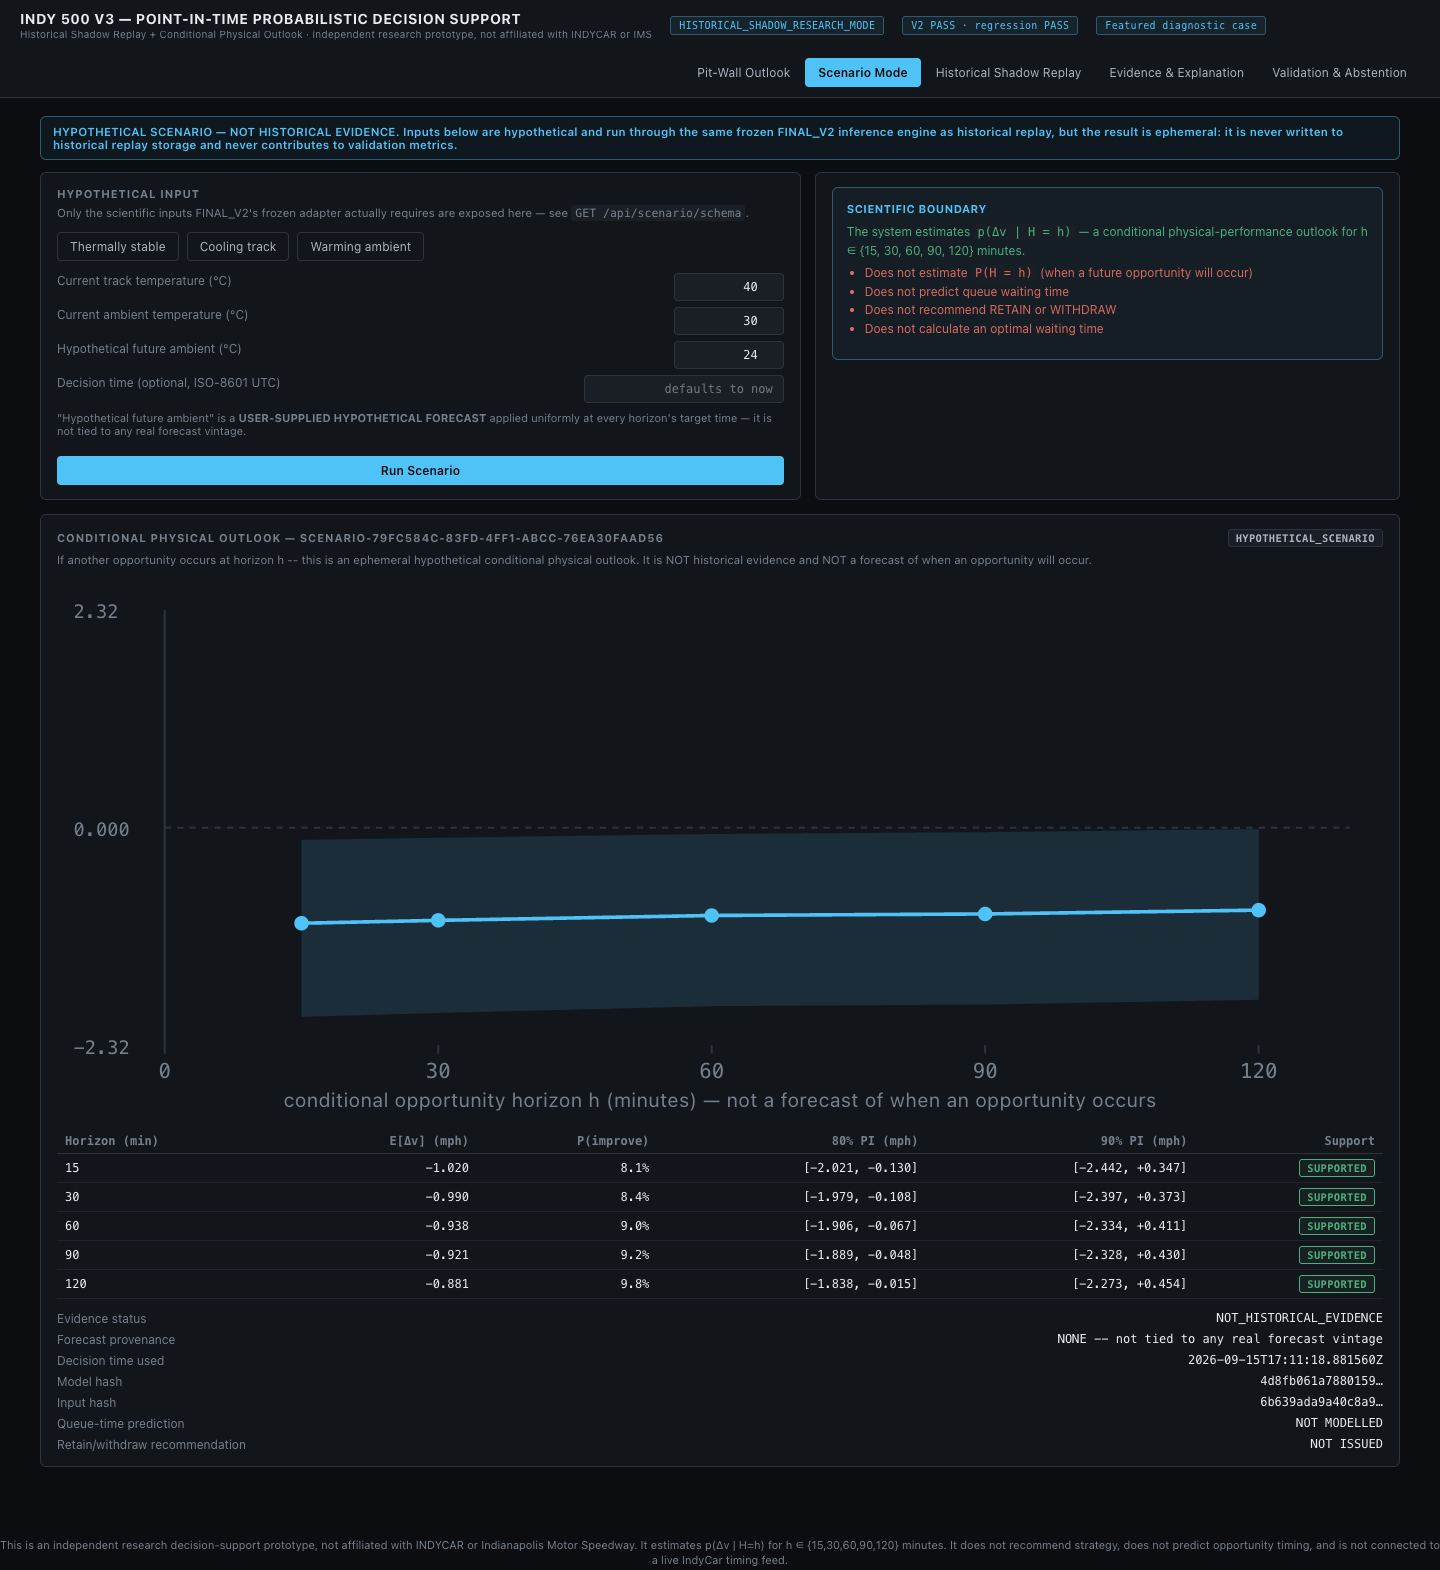
\includegraphics[width=0.92\textwidth]{figures/final_v3/figureD_ui_scenario_mode.png}
\caption{FINAL\_V3 Scenario Mode. The HYPOTHETICAL SCENARIO / NOT\_HISTORICAL\_EVIDENCE labelling is shown
prominently; queue-time prediction and retain/withdraw recommendation are both explicitly reported as absent.}
\label{fig:ui-scenario}
\end{figure}

References A. Colin Cameron, Jonah B. Gelbach, and Douglas L. Miller. Bootstrap-based improvements for inference with clustered errors. The Review of Economics and Statistics, 90(3):414--427, 2008. doi: 10.1162/rest.90. 3.414. Jiaqi Chen, Hao Wang, and Pengyu Xie. Pavement temperature prediction: Theoretical models and critical affecting factors. Applied Thermal Engineering, 158:113755, 2019. doi: 10.1016/j.applthermaleng.2019. 113755. Bradley Efron. Bootstrap methods: Another look at the jackknife. The Annals of Statistics, 7(1):1--26, 1979. doi: 10.1214/aos/1176344552. Tilmann Gneiting and Adrian E. Raftery. Strictly proper scoring rules, prediction, and estimation. Journal of the American Statistical Association, 102(477):359--378, 2007. doi: 10.1198/016214506000001437. Tilmann Gneiting, Fadoua Balabdaoui, and Adrian E. Raftery. Probabilistic forecasts, calibration and sharpness. Journal of the Royal Statistical Society: Series B, 69(2):243--268, 2007. doi: 10.1111/j.1467-9868. 2007.00587.x. Åke Hermansson. Mathematical model for paved surface summer and winter temperature: Comparison of calculated and measured temperatures. Cold Regions Science and Technology, 40(1--2):1--17, 2004. doi: 10.1016/j.coldregions.2004.03.001. Peter J. Huber. Robust estimation of a location parameter. The Annals of Mathematical Statistics, 35(1): 73--101, 1964. doi: 10.1214/aoms/1177703732.

INDYCAR. 2025 indianapolis 500 qualifications format, 2025. Official Indianapolis 500 qualifying procedure. INDYCAR. 2026 ntt indycar series rule book, 2026. See Rule 8.5: Indianapolis 500 Qualifications. D. P. Kelly and R. S. Sharp. Time-optimal control of the race car: Influence of a thermodynamic tyre model. Vehicle System Dynamics, 50(4):641--662, 2012. doi: 10.1080/00423114.2011.622406.

D. J. N. Limebeer, R. A. Dollar, S. Sivaramakrishnan, and N. Gordhan. Tyre and brake thermal management in nascar. Vehicle System Dynamics, 63(2):398--423, 2025. doi: 10.1080/00423114.2024.2342534. Ibrahim Reda and Afshin Andreas. Solar position algorithm for solar radiation applications. Technical Report NREL/TP-560-34302, National Renewable Energy Laboratory, 2008. Reuven Y. Rubinstein and Dirk P. Kroese. Simulation and the Monte Carlo Method. Wiley, 3 edition, 2016. doi: 10.1002/9781118631980. W. J. West and D. J. N. Limebeer. Optimal tyre management for a high-performance race car. Vehicle System Dynamics, 60(1):1--19, 2022. doi: 10.1080/00423114.2020.1802047.
